% Żeby nie było syfu to kolejne sekcje dodajemy do chapters/
% A potem includujemy za pomocą \input{chapters/...}

% Używamy \( \) i \[ \] zamiast dolarów -- tak jak się robi w LaTeXu

\documentclass[12pt, a4paper, polish, openany]{book}

% Please, let's familiarize ourselves with notatki.sty and tcs.sty so that we don't reinvent the wheel
\usepackage{notatki}
\fancyhead[L]{\textbf{\textit{MPI}}}

% Packages and commands used by the solutions copied from Probabil
\usepackage{zestawy}

% Only zestawy and tasks in the table of contents, some tasks have subsections and some don't
\setcounter{tocdepth}{1}

\begin{document}
% Front page and table of contents
\frontmatter

\begin{titlepage}

	\begin{center}
		\begin{figure}[h]
			\centering
			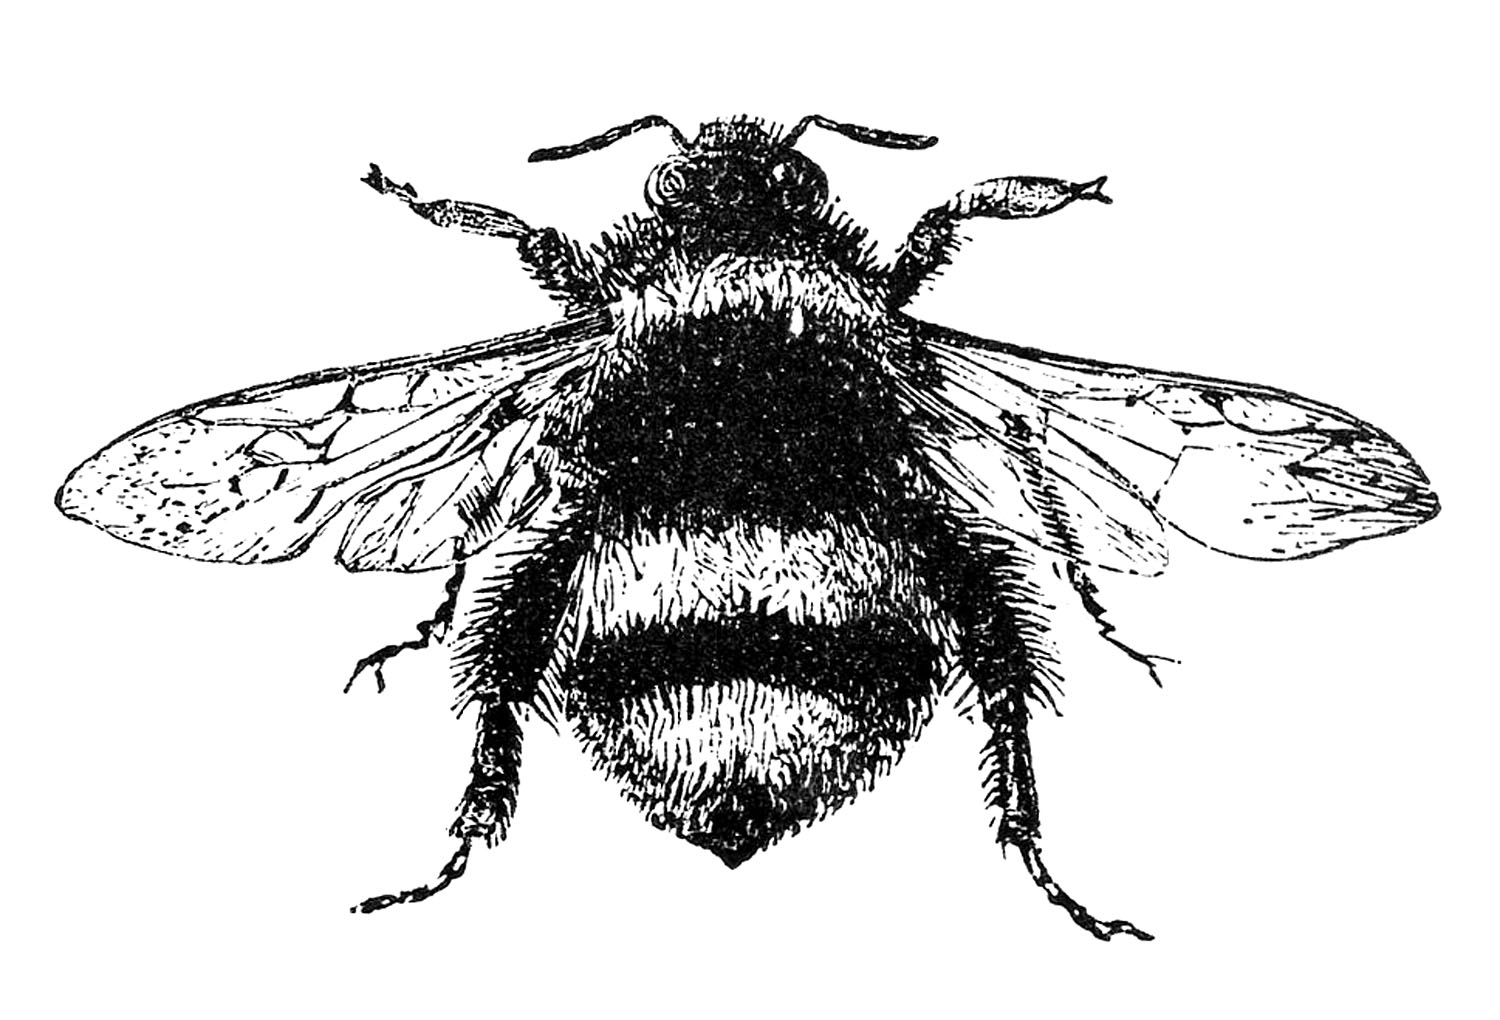
\includegraphics[scale=0.75]{img/bumblebee.jpg}
		\end{figure}
		\vspace{0.5cm}
		\Huge
		\textbf{\textsc{Metody Probabilistyczne Informatyki - Rozwiązania zestawów 2025}}

		\normalsize

		\line(1,0){330}

		\vspace{1cm}

		\textit{\textsc{Popełnione przez}}\\
		\vspace{5mm}

		\textbf{\textsc{
				Hubert Jastrzębski\\
				Mikołaj Kołek\\
				Dominik Korsa\\
				Filip Manijak\\
				Kacper Orszulak\\
				Oskar Prusik\\
				Aleksander Wieczorek\\
				Mateusz Wojaczek\\
			}}
		\vspace{5mm}

		\textit{oraz osoby, które zdecydowały się pozostać anonimowe}
		\vfill

		Kraków \\
		Anno Domini 2025

	\end{center}

\end{titlepage}


\tableofcontents
\section*{Licencja}
\begin{figure}[h]
	\begin{minipage}[c]{0.25\textwidth}
		
\includegraphics[width=0.7\textwidth]{img/licencja.png}
	\end{minipage}\hfill
	\begin{minipage}[c]{0.75\textwidth}
		\caption*{
			Ten utwór jest dostępny na
			\href{https://creativecommons.org/licenses/by-sa/4.0/}{licencji Creative Commons Uznanie autorstwa
				na tych samych warunkach 4.0 Międzynarodowe.}
		}
	\end{minipage}
\end{figure}

% Remove the "Rozdział x" chapter headings, as we already number our chapters
\titleformat{\chapter}[display]{\normalfont\Huge\bfseries}{}{0pt}{\Huge}
\titlespacing*{\chapter}{0pt}{0pt}{20pt}

% Chapters are titled "Zestaw N" and sections "Zadanie N", so don't number either of them
\setcounter{secnumdepth}{-1}

% Actual content
% Each zestaw sets a short \chaptermark, as the full titles don't fit in the page header
\mainmatter

\chapter{Zestaw 1 -- Aksjomaty, niezależność, wartość oczekiwana}
\chaptermark{Zestaw 1}
\graphicspath{{chapters/zestaw-01/}}
\section{Zadanie 1}
Wyprowadź z aksjomatów kolejne własności przestrzeni probabilistycznej

\subsection*{Aksjomaty miary probabilistycznej}
\begin{itemize}
	\item \(P \colon \mathcal F \to [0, \infty)\)
	\item \(P(\Omega) = 1\)
	\item jeśli \(\{A_n\}_{n\in\mathbb N}\) jest (przeliczalną!) rodziną
	      zbiorów parami rozłącznych,\\ to
	      \(P(\bigcup_{n\in\mathbb N} A_n) = \sum_{n\in\mathbb N} P(A_n)\)
\end{itemize}

\subsection*{Rozwiązanie}
\begin{enumerate}
	\item[(i)]
	      \(P(\emptyset) = 0\)\\
	      \(\{\Omega, \emptyset, \emptyset, \emptyset, \emptyset, \ldots\}\)
	      jest przeliczalną rodziną zbiorów parami rozłącznych\\
	      Z aksjomatów:\\
	      \(
	      P(\Omega \cup \emptyset \cup \emptyset \cup \ldots) =
	      P(\Omega) + P(\emptyset) + P(\emptyset) + \ldots
	      \)\\
	      \(
	      P(\Omega) =
	      P(\Omega) + P(\emptyset) + P(\emptyset) + \ldots
	      \)\\
	      \(
	      1 = 1 + P(\emptyset) + P(\emptyset) + \ldots
	      \)\\
	      \(
	      0 = \sum_{n\in\mathbb N} P(\emptyset)
	      \)\\
	      \(
	      P(\emptyset) = 0
	      \)\\
	      Korzystając z tej tożsamości będziemy od tej pory mogli używać
	      aksjomatu 3. w wersji skończonej - nieskończenie wiele zbiorów
	      pustych nie zmieni wyniku.

	\item[(ii)]
	      \(P(\Omega\setminus A) = 1 - P(A)\)\\
	      \(\{(\Omega\setminus A), A\}\) to skończona rodzina zbiorów parami rozłącznych.
	      W zgodzie z aksjomatem powinniśmy w niej uwzględnić jeszcze nieskończenie
	      wiele zbiorów pustych\\
	      \(P((\Omega\setminus A) \cup A) = P(\Omega\setminus A) + P(A)\)\\
	      \(P(\Omega) = P(\Omega\setminus A) + P(A)\)\\
	      \(P(\Omega\setminus A) = P(\Omega) - P(A)\)\\
	      \(P(\Omega\setminus A) = 1 - P(A)\)

	\item[(iii)]
	      jeśli \(A \subseteq B\), to \(P(B\setminus A) = P(B) - P(A)\)\\
	      \((B\setminus A), A\) są rozłączne:\\
	      \(P((B\setminus A)\cup A) = P(B\setminus A) + P(A)\)\\
	      \(P(B) = P(B\setminus A) + P(A)\)\\
	      \(P(B\setminus A) = P(B) - P(A)\)

	\item[(iv)]
	      jeśli \(A \subseteq B\), to \(P(A) \leqslant P(B)\)\\
	      korzystając z (iii): \(P(B) = P(A) + P(B\setminus A)\)\\
	      z aksjomatu \(P\) przyjmuje wartości nieujemne:
	      \(P(B\setminus A) \geqslant 0\)\\
	      \(P(B) = P(A) + P(B\setminus A) \geqslant P(A)\)

	\item[(v)]
	      \(P(A) \leqslant 1\)\\
	      korzystamy z (ii): \(P(A) = 1 - P(\Omega\setminus A)\)\\
	      \(P\) przyjmuje wartości nieujemne: \(P(\Omega\setminus A) \geqslant 0\)\\
	      \(P(A) = 1 - P(\Omega\setminus A) \leqslant 1\)

	\item[(vi)]
	      \(P(A\cup B) = P(A) + P(B) - P(A\cap B)\)\\
	      Zauważmy \(P(B) = P(B\setminus A) + P(A\cap B)\)\\
	      \(P(A\cup B) = P(A) + P(B\setminus A) = P(A) + P(B) - P(A\cap B)\)
\end{enumerate}

\section{Zadanie 2}
Jeśli \({A_n}_{n\in \mathbb{N}}\) jest występującą rodziną zdarzeń, czyli
\(A_0 \subseteq A_1 \subseteq A_2 \subseteq \ldots\), to:
\[
	P\left(\bigcup_{n=0}^{\infty} A_n\right) = \lim_{n \to \infty} P(A_n)
\]

Jeśli \({A_n}_{n\in \mathbb{N}}\) jest zstępującą rodziną zdarzeń, czyli
\(A_0 \supseteq A_1 \supseteq A_2 \supseteq \ldots\), to:
\[
	P\left(\bigcap_{n=0}^{\infty} A_n\right) = \lim_{n \to \infty} P(A_n)
\]


\subsection*{Rozwiązanie}
Tak to prawda XD;

\subsubsection*{Dowód}
Poniżej podamy dowody dla obu stwierdzeń. W obu przypadkach skorzystamy z prostych własności miary prawdopodobieństwa oraz definicji granicy ciągu liczb rzeczywistych (epsilon -- delta, tu: epsilon i indeks \(N\)).

\paragraph{1) Rodzina rosnąca: \(A_0\subseteq A_1\subseteq\ldots\)}

Niech \(A=\bigcup_{n=0}^{\infty}A_n\). Wykazujemy,
\[P(A)=\lim_{n\to\infty}P(A_n).\]

Ponieważ \(A_n\subseteq A_{n+1}\) dla każdego \(n\), ciąg \(P(A_n)\) jest niemalejący i ograniczony z góry przez \(1\), a zatem ma granicę (można to przyjmować jako \(L:=\lim_{n\to\infty}P(A_n)\) lub jako \(\sup_n P(A_n)\)). Pokażemy, że \(P(A)=L\).

Zauważmy, że zbior \(A\) jest sumą rozłącznych przyrostów:
\[A=\bigcup_{n=0}^{\infty}A_n= A_0\uplus (A_1\setminus A_0)\uplus (A_2\setminus A_1)\uplus\cdots,\]
gdzie symbolem \(\uplus\) oznaczamy rozłączność w sensie rozłożenia na zbiory parami rozłączne.

Dla dowolnego \(m\) mamy
\[A_m = A_0\uplus (A_1\setminus A_0)\uplus\cdots\uplus (A_m\setminus A_{m-1}).\]
Korzystając z addytywności prawdopodobieństwa na zbiorach parami rozłącznych dostajemy
\[P(A_m)=P(A_0)+\sum_{k=1}^m P(A_k\setminus A_{k-1}).\]
Jeśliśmy dla \(m\to\infty\), to z monotoniczności i jednoczesnej nieujemności wyrazów szeregu mamy
\[\lim_{m\to\infty}P(A_m)=P(A_0)+\sum_{k=1}^{\infty} P(A_k\setminus A_{k-1}).\]
Równocześnie
\[P(A)=P\Big(\biguplus_{k=0}^{\infty} (A_k\setminus A_{k-1})\Big)=P(A_0)+\sum_{k=1}^{\infty} P(A_k\setminus A_{k-1}),\]
stąd \(P(A)=\lim_{n\to\infty}P(A_n)\).

Można to również sformalizować bez rozkładu na przyrosty, używając definicji granicy: dla danego \(\varepsilon>0\) niech \(L=\lim_{n}P(A_n)=\sup_n P(A_n)\). Istnieje indeks \(N\) taki, że dla \(n\ge N\) mamy \(P(A_n)>L-\varepsilon\). Ponieważ \(A_n\uparrow A\), to \(A\setminus A_n\downarrow\emptyset\) i z podzielności miary \(P(A)-P(A_n)=P(A\setminus A_n)\to0\), skąd \(P(A)=L\).

\paragraph{2) Rodzina malejąca: \(A_0\supseteq A_1\supseteq A_2\supseteq\ldots\)}

Niech \(A=\bigcap_{n=0}^{\infty}A_n\). Zakładamy dodatkowo, że istnieje \(k\) takie, że \(P(A_k)<\infty\) (w kontekście probabilistycznym zwykle \(P\) jest miarą skończoną i ta hipoteza jest automatycznie spełniona). Chcemy pokazać, że
\[P(A)=\lim_{n\to\infty}P(A_n).\]

Rozważmy zbiory \(B_n:=A_0\setminus A_n\). Ponieważ \(A_n\) jest malejący, to \(B_n\) jest rosnący i
\[\bigcup_{n=0}^{\infty}B_n = A_0\setminus\bigcap_{n=0}^{\infty}A_n = A_0\setminus A.\]
Z pierwszej części dowodu (ciągi rosnące) mamy
\[P\Big(\bigcup_{n=0}^{\infty}B_n\Big)=\lim_{n\to\infty}P(B_n).
\]
Ale \(P(B_n)=P(A_0)-P(A_n)\) dla każdego \(n\) (ponieważ \(B_n\) i \(A_n\) rozdzielają \(A_0\)), stąd
\[P(A_0)-P(A)=\lim_{n\to\infty}\bigl(P(A_0)-P(A_n)\bigr)=P(A_0)-\lim_{n\to\infty}P(A_n).
\]
Po uproszczeniu otrzymujemy \(P(A)=\lim_{n\to\infty}P(A_n)\), co kończy dowód.

\paragraph{Uwaga o hipotezie skończoności:} Jeśli \(P(A_0)=\infty\) (nie jest to sytuacja typowa dla prawdopodobieństwa, ale może wystąpić dla ogólnych miar), to równanie \(P(B_n)=P(A_0)-P(A_n)\) nie ma sensu; w teorii miar stosuje się wtedy warunek, że istnieje przynajmniej jeden indeks \(k\) z \(P(A_k)<\infty\), co umożliwia analogiczny argument na przesunietym ciągu.




\section{Zadanie 3}
\autor{Dominik Korsa}

Udowodnij, że dla dowolnego ciągu \(A_0, A_1\), ... zachodzi:

\[
	P(\bigcup_{n = 0}^{\infty} A_n) \leq \sum_{n = 0}^{\infty} P(A_n)
\]

\subsection*{Rozwiązanie}
Definiujemy nowy ciąg \textbf{rozłącznych zdarzeń}:
\(\displaystyle
B_n = A_n \setminus \bigcup_{i = 0}^{n-1} A_i
\).

Można pokazać, że:
\(\displaystyle
\bigcup_{n \in \mathbb{N}} B_n = \bigcup_{n \in \mathbb{N}} A_n
\).

\begin{align*}
	P\left(\bigcup_{n \in \mathbb{N}} A_n\right)
	 & = P\left(\bigcup_{n \in \mathbb{N}} B_n\right) \\
	 & = \sum_{n \in \mathbb{N}} P(B_n)               \\
	 & \leq \sum_{n \in \mathbb{N}} P(A_n)
\end{align*}
Pierwsze przejście mamy z definicji miary probabilistycznej, dzięki temu że
zdarzenia w rodzinie \(\{B_n\}\) są parami rozłączne.

Nierówność mamy, bo dla każdego \(n \in \mathbb{N}\) mamy \(B_n \subseteq A_n\), więc \(P(B_n) \leq P(A_n)\).

Otrzymana nierówność kończy dowód.

\section{Zadanie 4}
Niech \(A_0, A_1, \dots\) będzie nieskończonym ciągiem zdarzeń i
niech \(P(A_n) = 1\) dla każdego \(n\).
Udowodnij, że \(P(\bigcap_{n=0}^{\infty}A_n) = 1\)

\subsection*{Rozwiązanie}
Dla każdego n mamy \(P(A_n) = 1\), więc dla każdego dopełnienia zdarzenia \(A'_n = \Omega - A_n\) mamy:
\(P(A'_n) = 1 - P(A_n) = 0\).

Zauważmy, że dopełnienie przecięcia jest równe sumie dopełnień
\[
	(\bigcap_{n=0}^{\infty}A_n)' = \bigcup_{n=0}^{\infty}A_n'
\]
Teraz korzystamy z nierówności pomiędzy prawdopodobieństwem sumy a sumą prawdopodobieństw (Zadanie 3),
z czego ładnie nam wychodzi teza
\[
	P(\bigcup_{n=0}^{\infty}A_n') \leq \Sigma_{n=0}^{\infty}P(A'_n) = \Sigma_{n=0}^{\infty}0 = 0
\]
\[
	P(\bigcup_{n=0}^{\infty}A_n') = 0
\]
\[
	P(\bigcap_{n=0}^{\infty}A_n) = 1 - 0 = 1
\]

\section{Zadanie 5}
\autor{Filip Manijak}
Podaj przykład zdarzeń $X, Y, Z$, takich że każde dwa są niezależne, ale cała trójka nie jest niezależna. Podaj przykład $n+1$ zdarzeń takich, że każde $n$ z nich są niezależne, ale wszystkie $n+1$ są zależne.

\subsection*{Rozwiązanie}
Przykład dla 3: 
Mamy zdarzenia elementarne (równie prawdopodobne i niezależne) $A_1, A_2, A_3, A_4$. Wtedy: 
$$X = A_1 \cup A_2; Y = A_1 \cup A_3; Z = A_1 \cup A_3$$
Widzimy, że prawdopodobieństwo $P(X)=P(Y)=P(Z) = 0.5$, oraz prawdopodobieństwa $P(X \cap Y) = P(Z \cap X)= P(Y \cap Z) = 0.25 = P(X) \cdot P(Y)$, czyli działa. Jednak $P(X\cap Y \cap Z) = 0.25 \neq (0.5)^3$.

Przykład dla $n+1$
Jako przestrzeń zdarzeń elementarnych bierzemy punkty kostki $\{0,1\}^n$. Teraz definiujemy zdarzenia:
$X_1, ... X_n$ jako zdarzenia zachodzące, gdy punkt ma $i$-tą współrzędną równą 1, oraz $Y$ jako zachodzące jeżeli suma współrzędnych jest parzysta. Łatwo zauważyć że $P(X_1 \cap ...\cap X_n) = P(X_1) \cdot ... \cdot P(X_n)$ oraz że prawdopodobieństwo każdego podzbioru $n-1$ $X$-ów ($Z$) i $Y$ też spełnia: $P(Z \cap Y) = P(Z)\cdot P(Y)$. Jednak prawdopodobieństwo wszystkiego razem: $P(X_1 \cap ...\cap X_n \cap Y) \neq (0.5)^{n+1}$ ponieważ w świecie zawierającym $2^n$ elementów (równieprawdopodobnych!!!) żadne zdarzenie nie może mieć takie prawdopodobieństwa (gdyby miało, to $P(\Omega) \leq P(X_1 \cap ...\cap X_n \cap Y)*2^n = 0.5 \neq 1$ (z prawdopodobieństwa sumy).

\section{Zadanie 6 (Mateusz Wojaczek)}
Pokaż, że jeżeli zdarzenia $A_1, A_2, \ldots, A_n$ są niezależne, 
to zdarzenia 
\[
\Omega \setminus A_1,\, \Omega \setminus A_2,\, \ldots,\, \Omega \setminus A_n
\]
również są niezależne.

\subsection*{Rozwiązanie}

\subsection*{Założenie (niezależność zdarzeń $A_1, \dots, A_n$)}

\[
\forall I \subseteq \{1,2,\dots,n\}, \quad
P\!\left(\bigcap_{i \in I} A_i \right) = \prod_{i \in I} P(A_i).
\]

\subsection*{Teza do udowodnienia}

Dla dowolnego $I \subseteq \{1, \dots, n\}$ zachodzi
\[
P\!\left(\bigcap_{i \in I} (\Omega \setminus A_i)\right)
= \prod_{i \in I} P(\Omega \setminus A_i).
\]

\subsection*{Dowód}

Niech $I \subseteq [n]$. Rozpoczynamy od przekształcenia przecięcia dopełnień przy użyciu prawa De Morgana:

\begin{align*}
P\!\left( \bigcap_{i \in I} (\Omega \setminus A_i) \right)
&= P\!\left( \Omega \setminus \bigcup_{i \in I} A_i \right) 
\text{(De Morgan)} \\
&= P(\Omega) - P\!\left( \bigcup_{i \in I} A_i \right) 
= 1 - P\!\left( \bigcup_{i \in I} A_i \right).
\end{align*}


\[
P\!\left( \bigcap_{i \in I} (\Omega \setminus A_i) \right)
= 1 - \sum_{\substack{J \subseteq I \\ J \neq \emptyset}} (-1)^{|J|+1} P\!\left( \bigcap_{i \in J} A_i \right).
\]

Ponieważ zdarzenia $A_i$ są niezależne

\[
P\!\left( \bigcap_{i \in J} A_i \right) = \prod_{i \in J} P(A_i),
\]

więc

\[
P\!\left( \bigcap_{i \in I} (\Omega \setminus A_i) \right)
= 1 - \sum_{\substack{J \subseteq I \\ J \neq \emptyset}} (-1)^{|J|+1} \prod_{i \in J} P(A_i).
\]

Teraz zauważamy, że suma odpowiada funkcji tworzącej iloczynu:

\[
\sum_{\substack{J \subseteq I \\ J \neq \emptyset}} (-1)^{|J|+1} \prod_{i \in J} P(A_i)
= 1 - \prod_{i \in I} \big( 1 - P(A_i) \big).
\]

Podstawiając to, otrzymujemy:

\begin{align*}
P\!\left( \bigcap_{i \in I} (\Omega \setminus A_i) \right)
&= 1 - \left[ 1 - \prod_{i \in I} \big( 1 - P(A_i) \big) \right] \\
&= \prod_{i \in I} \big( 1 - P(A_i) \big) \\
&= \prod_{i \in I} P(\Omega \setminus A_i).
\end{align*}


\subsection*{Odpowiedź}
\[
\hfill \square
\]

\section{Zadanie 7 (Aleksander Wieczorek)}
Niech $A_0,A_1,\dots$ będzie nieskończonym ciągiem zdarzeń i niech $P(\Omega-A_n)\le \frac{1}{3^n}$ dla każdego $n$. Uzasadnij, że
$$P(\bigcap_{n=1}^\infty A_n) \ge \frac{1}{2}$$
\subsection*{Rozwiązanie}
Na początku musimy zauważyć, że:
$$\Omega-\bigcap_{n=1}^\infty A_n=\bigcup_{n=1}^\infty (\Omega-A_n)$$
Najprościej jest to narysować i "to widać". Machając rękami możemy powiedzieć, że prawa strona dla każdego i bierze wszystko co nie leży w $A_i$.
Po zsumowaniu okaże się, że dostaniemy wszystko oprócz przecięcia, czyli lewą stronę.\\
Dalsza część jest już dosyć prosta.\\
Korzystając z powyższej obserwacji dostaniemy: 
$$P(\Omega-\bigcap_{n=1}^\infty A_n)=P(\bigcup_{n=1}^\infty (\Omega-A_n))$$
co daje:
$$1-P(\bigcap_{n=1}^\infty A_n)=P(\bigcup_{n=1}^\infty (\Omega-A_n))$$
$$1-P(\bigcup_{n=1}^\infty (\Omega-A_n))=P(\bigcap_{n=1}^\infty A_n)$$
Teraz przekształcamy tezę:
$$P(\bigcap_{n=1}^\infty A_n) \ge \frac{1}{2}$$
$$1-P(\bigcup_{n=1}^\infty (\Omega-A_n))\ge \frac{1}{2}$$
$$P(\bigcup_{n=1}^\infty (\Omega-A_n))\le \frac{1}{2}$$
Teraz wystarczy tylko pokazać, że $P(\bigcup_{n=1}^\infty (\Omega-A_n))\le \frac{1}{2}$. Z zadania 3. wiemy, że 
$$P(\bigcup_{n=0}^\infty A_n) \le \sum_{n=0}^\infty P(A_n)$$
teraz obliczmy naszą sumę korzystając z $P(\Omega-A_n)\le \frac{1}{3^n}$:
$$\sum_{n=0}^\infty P(\Omega - A_n)\le \frac{1}{3}+\frac{1}{9}+\dots = \frac{\frac{1}{3}}{1-\frac{1}{3}}=\frac{1}{2}$$
Co daje:
$$P(\bigcup_{n=0}^\infty (\Omega-A_n)) \le \sum_{n=0}^\infty P(A_n)\le \frac{1}{2}$$



\section{Zadanie 8 (Oskar Prusik)}
Do N ponumerowanych listów wkładamy losowo N liczb. Jakie jest prawdopodobieństwo, że żadna liczba nie trafi do odpowiedniego listu?

\subsection*{Rozwiązanie}
Całe zadanie to jest dosłownie zasada włączeń i wyłączeń.

Niech $A_i$ - zdarzenie, że $i$-ta liczba trafiła do $i$-tego listu (dla $i = 1, 2, \ldots, N$).

Z zasady włączeń i wyłączeń:
\[
\left| \bigcup_{i=1}^N A_i \right| = \sum_{\substack{I \subseteq [N] \\ I \neq \emptyset}} (-1)^{|I| + 1} \left| \bigcap_{i \in I} A_i \right|
\]

\subsection*{Obliczenie mocy przekrojów}

Dla ustalonego $I \subseteq [N]$ z $|I| = k$:
\[
\left| \bigcap_{i \in I} A_i \right| = (N-k)!
\]
ponieważ jeśli $k$ liczb jest na swoich miejscach, to pozostałe $N-k$ liczb można rozmieścić dowolnie.

Liczba takich podzbiorów $I$ to $\binom{N}{k}$, więc:
\[
\sum_{\substack{I \subseteq [N] \\ |I| = k}} \left| \bigcap_{i \in I} A_i \right| = \binom{N}{k} (N-k)!
\]

\subsection*{Moc zdarzenia że przynajmniej jedna liczba trafiła dobrze}

\[
\left| \bigcup_{i=1}^N A_i \right| = \sum_{k=1}^N (-1)^{k+1} \binom{N}{k} (N-k)!
\]

\subsection*{Prawdopodobieństwo że przynajmniej jedna liczba trafiła dobrze}

\[
P\left( \bigcup_{i=1}^N A_i \right) = \frac{\left| \bigcup_{i=1}^N A_i \right|}{N!} 
= \sum_{k=1}^N (-1)^{k+1} \frac{ \binom{N}{k} (N-k)!}{N!}
 = \sum_{k=1}^N (-1)^{k+1} \frac{1}{k!}
\]

\subsection*{Prawdopodobieństwo że żadna liczba nie trafiła dobrze}

\[
P\left( \text{żadna liczba nie trafiła do odpowiedniego listu} \right) = 1 - P\left( \bigcup_{i=1}^N A_i \right)
\]

\[
P\left( \text{żadna liczba nie trafiła do odpowiedniego listu} \right) = 1 - \sum_{k=1}^N (-1)^{k+1} \frac{1}{k!} = \sum_{k=0}^N \frac{(-1)^k}{k!}
\]

\subsection*{Odpowiedź}
\[
\boxed{ \sum_{k=0}^N \frac{(-1)^k}{k!} }
\]

\section{Zadanie 9}
Niech \(q \in \{0, 1\}^{19}\) będzie arbitralnie wybranym \(19\)-elementowym ciągiem zer i jedynek. Rzucamy wielokrotnie symetryczną monetą (tj. taką, że orzeł i reszka wypadają z jednakowym prawdopodobieństwem) i notujemy rezultaty tworząc w ten sposób ciąg. Jeśli wypadł orzeł notujemy 0, jeśli reszka 1. Jakie jest prawdopodobieństwo, że ciąg \(q\) wystąpi (być może po wielu rzutach) jako spójny podciąg notowanego ciągu?

\subsection*{Rozwiązanie}

Intuicja podpowiada, że prawdopodobieństwo to będzie wynosić 1, ale nie jest raczej tak prosto dotrzeć do tego bezpośrednio. Zamiast liczyć prawdopodobieństwo wystąpienia ciągu \(q\) przy rzucaniu pojedynczymi monetami, znacznie łatwiej będzie liczyć prawdopodobieństwo, jeśli będziemy rzucać blokami po 19. A konkretniej:

\(B\) - zdarzenie polegające na tym, że w ciągu wystąpił ciąg \(q\) po pewnej liczbie rzutów.

\(B_i\) - zdarzenie polegające na tym, że w ciągu pierwszych \(i\) lub mniej serii rzutów po 19 monet, któraś z serii była ciągiem \(q\).

Zauważmy, że \(\{B_i\}_{i\in\mathbb{N}}\) jest wstępującą rodziną zdarzeń (patrz zad. 2) oraz suma po tej rodzinie implikuje zdarzenie B. Wyliczamy także prawdopodobieństwo zdarzenia \(B_i\) poprzez zdarzenie przeciwne. Wystarczy połączyć to wszystko następująco:

\begin{align*}
	P(B_n)                                & = 1 - \left[1 - \left(\frac 1 2\right)^{19}\right]^n                                     \\
	P(\bigcup_{n=1}^\infty B_n)           & = \lim_{n \to \infty}\left(1 - \left[1 - \left(\frac 1 2\right)^{19}\right]^n\right) = 1 \\
	(\bigcup_{n=1}^\infty B_n \implies B) & \implies P(\bigcup_{n=1}^\infty B_n) \leq P(B)                                           \\
	1 \leq P(B)                           & \leq 1                                                                                   \\
	P(B)                                  & = 1
\end{align*}

\subsection*{Odpowiedź}
\[
	\boxed{\text{P(B) = 1}}
\]

\section{Zadanie 10}
\autor{Mikołaj Kołek}

Startujemy doświadczenie z liczbą \(k\) (\(0 \leq k \leq n\)). Barierami są liczby \(0\) i \(n\). Dopóki aktualna liczba nie jest jedną z barier do aktualnej liczby dodajemy \(1\) lub \(-1\) z równym prawdopodobieństwem. Jakie jest prawdopodobieństwo, że spacer uderzy w którąś z barier? Jakie jest prawdopodobieństwo, że spacer uderzy w \(n\)?

\subsection*{Rozwiązanie}
Pierwsze rozwiążmy prostszą część, czyli prawdopodobieństwo uderzenia w dowolną z barier. Możemy zauważyć, że jeśli w naszym ciągu jedynek i minus jedynek pojawi się w jakiejkolwiek chwili \(n - 1\) jedynek pod rząd, to wiemy, że ten ciąg na pewno uderza w którąś z barier. Zadanie to sprowadza się więc do zadania 9, z którego wiemy, że prawdopodobieństwo wystąpienia takiego ciągu jedynek w naszym ciągu wynosi 1.

Teraz rozważmy prawdopodobieństwo, że spacer uderzy w \(n\). Niech:

\(X_i\) - zdarzenie polegające na tym, że spacer uderzył w \(n\) dla \(k = i\).

Można zauważyć, że \(P(X_0) = 0\), bo dla \(k = 0\) spacer natychmiastowo uderza w barierę \(0\), a \(P(X_n) = 1\), bo dla \(k = n\) spacer od razu uderza w \(n\). Dodatkowo możemy zauważyć, że:

$$ \forall_{i \in [n-1]} P(X_i) = \frac{P(X_{i-1})}{2} + \frac{P(X_{i+1})}{2} $$

Używając tego wzoru, możemy teraz policzyć stosunek \(P(X_1)\) do \(P(X_2)\), później \(P(x_2)\) do \(P(x_3)\), itd. Udowodnię indukcyjnie, że \(P(X_i) = \frac{i}{i+1} P(X_{i+1})\). Baza indukcji:

$$ P(X_1) = \frac{P(X_{0})}{2} + \frac{P(X_{2})}{2} = \frac{P(X_{2})}{2} $$

Krok indukcyjny:
$$ P(X_i) = \frac{i}{i+1} P(X_{i+1}) $$
$$ P(X_{i+1}) = \frac{P(X_{i})}{2} + \frac{P(X_{i+2})}{2} = \frac{iP(X_{i+1})}{2i +2} + \frac{P(X_{i+2})}{2}$$
$$ \frac{P(X_{i+1})(i+2)}{2i+2} = \frac{P(X_{i+2})}{2} $$
$$ P(X_{i+1}) = \frac{P(X_{i+2})}{2} \frac{2i+2}{i+2} = \frac{i+1}{i+2} P(X_{i+2}) $$

W takim razie, zachodzi:
$$ P(X_i) = \frac{i}{i+1} P(X_{i+1}) = \frac{i}{i+1}\frac{i+1}{i+2} P(X_{i+2}) = \frac{i}{i+1} \frac{i+1}{i+2} \ldots \frac{n-1}{n} P(X_n) = \frac{i}{n} P(X_n) = \frac{i}{n}  $$

A więc dla ustalonego \(k\), prawdopodobieństwo, że spacer uderzy w \(n\) to \(\frac{k}{n}\).

\subsection*{Odpowiedź}
\[
\boxed{\text{Prawdopodobieństwo, że spacer uderzy w którąś z barier = 1}}
\]
\[
\boxed{\text{Prawdopodobieństwo, że spacer uderzy w \(n\) = \(\frac{k}{n}\)}}
\]
\section{Zadanie 11}
W urnie znajdują się dwie kule: jedna czarna i jedna biała. W każdej z \(n-2\) rund losujemy w sposób jednostajny jedną kulę z urny i dokładamy do urny kulę o tym samym kolorze co wylosowana. Pokaż, że liczba białych kul w urnie na końcu jest z jednakowym prawdopodobieństwem jedną z liczb ze zbioru \([n-1].\)

\subsection*{Rozwiązanie}
\(k\) – końcowa liczba białych kul w urnie.\\[1em]

Wszystkich możliwości losowania mamy \((n-1)!\) (najpierw losujemy z 2 kul, później z 3 itd. aż do \(n-1\)).\\[1em]

Policzymy teraz, ile jest możliwości losowań, aby końcowo liczba białych kul w urnie była równa \(k\).\\[0.5em]

\begin{itemize}
	\item \(\displaystyle \binom{n-2}{k-1}\) – wybór rund, w których wylosowano białe kule,\\
	\item \((k-1)!\) – możliwości wylosowania białych kul,\\
	\item \((n-k-1)!\) – możliwości wylosowania czarnych kul.
\end{itemize}

Zatem prawdopodobieństwo, że na koniec w urnie będzie \(k\) białych kul wynosi:
\[
	\frac{\binom{n-2}{k-1} (k-1)! (n-k-1)!}{(n-1)!}
	= \frac{(n-2)! (k-1)! (n-k-1)!}{(k-1)! (n-k-1)! (n-1)!}
	= \frac{1}{n-1}.
\]

Niezależnie od wartości \(k\), prawdopodobieństwo wynosi \(\dfrac{1}{n-1}\).

\section{Zadanie 12}
\autor{Dominik Korsa \& Hubert Jastrzębski}
(Bratobójczy pojedynek) Król Artur urządza turniej rycerski, w którym rycerze walczą w systemie turniejowym (jakże by inaczej?).  
Uczestnicy każdego pojedynku mają równe szanse na zwycięstwo. Drabinka turnieju jest układana losowo.  

Wśród $2^n$ uczestników jest dwóch braci.  
Jakie jest prawdopodobieństwo, że spotkają się w pojedynku?

\subsection*{Rozwiązanie}
Niech $\{A_i\}_{i \in \{0,\dots,n-1\}}$ to rodzina parami rozłącznych zdarzeń, gdzie $A_i$ to zdarzenie, że bracia spotkają się w swoim $i+1$ pojedynku.  

Wówczas
\[
P(A_i) = \frac{2^i}{2^n-1} \cdot \left(\frac{1}{2}\right)^i \cdot \left(\frac{1}{2}\right)^i
= \frac{2^{-i}}{2^n-1}.
\]

\noindent
Pierwszy czynnik $\frac{2^i}{2^n-1}$ to prawdopodobieństwo, że drugi brat znalazł się w odpowiednim miejscu w drabince -- jest $2^n-1$ możliwych miejsc, a $2^i$ z nich prowadzi do pojedynku na poziomie $i+1$ (wchodzimy $i$ poziomów do góry, przechodzimy do sąsiada i patrzymy na liście jego poddrzewo, które ma $i$ poziomów).  

Pozostałe dwa czynniki $\left(\frac12\right)^i \cdot \left(\frac12\right)^i$ to prawdopodobieństwa, że obaj bracia wygrają wszystkie wcześniejsze pojedynki, aby dotrzeć do pojedynku $i+1$ 
(zakładamy niezależność pojedynków i równą szansę każdego uczestnika -- stąd można wymnożyć prawdopodobieństwa).

\textbf{Przykład} 
Dla $n=3$ i $i=2$, czyli jest $2^3=8$ uczestników, bracia spotykają się w 3. pojedynku:
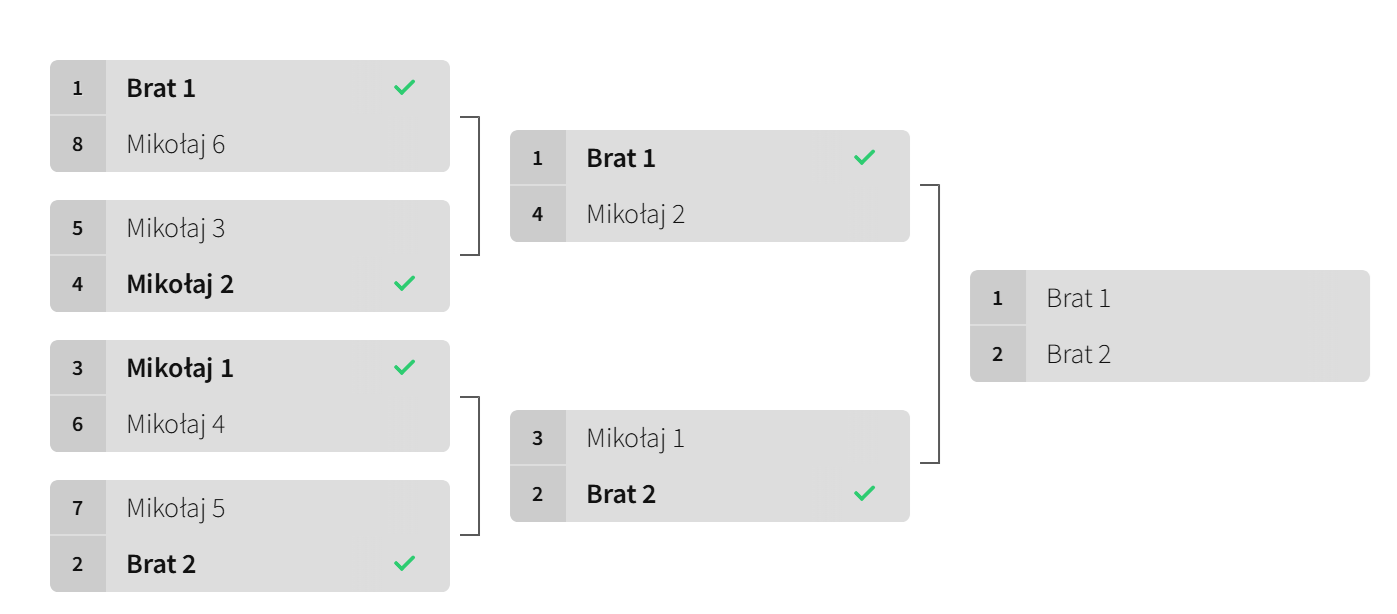
\includegraphics[width=0.7\textwidth]{tasks/12_01.png}

Jest $2^i=4$ miejsc, które prowadzą do pojedynku 3, które wcześniej nie walczą z bratem 1.

Jest $2^n-1=2^3-1=7$ możliwych miejsc dla brata 2 (wszystkie poza miejscem brata 1).

Dodatkowo, aby bracia spotkali się w 3. pojedynku, obaj muszą wygrać swoje wcześniejsze pojedynki (po 2 zwycięstwa każdy), 
co zdarza się z prawdopodobieństwem $\left(\frac12\right)^2 \cdot \left(\frac12\right)^2$.

Stąd w tym przypadku: 
\[P(A_2) = \frac{2^i}{2^n-1} \cdot \left(\frac{1}{2}\right)^i \cdot \left(\frac{1}{2}\right)^i = \frac{4}{7} \cdot \frac{1}{4} \cdot \frac{1}{4} = \frac{1}{28}\]

Ostatecznie zdarzenie $A$, że bracia spotkają się w turnieju, to
\[
A = \bigcup_{i = 0}^{n-1} A_i,
\]
więc
\[
P(A) = \sum_{i = 0}^{n-1} P(A_i) 
= \frac{1}{2^n-1} \sum_{i=0}^{n-1} 2^{-i} 
= \frac{2(1-2^{-n})}{2^n-1} 
= \boxed{2^{1-n}}.
\]

\subsection*{Odpowiedź}
\[
\boxed{2^{1-n}}
\]
\section{Zadanie 13 (Dominik Korsa)}
Dana jest moneta asymetryczna, która z nieznanym Ci prawdopodobieństwem
\(p \in (0, 1)\) zwraca orła i z prawdopodobieństwem \(1 - p\) zwraca reszkę.
Zaproponuj algorytm, który będzie symulował zachowanie monety symetrycznej,
to znaczy z prawdopodobieństwem \(\frac{1}{2}\) zwróci orła bądź reszkę.
Jedyne co możesz robić to rzucać monetą asymetryczną i na bazie obserwowanych
rezultatów kontynuować rzucanie bądź przerwać i zwrócić wynik.
Jaka jest oczekiwana liczba rzutów monetą asymetryczną przed zwróceniem wyniku?
Wynik podaj jako funkcję \(p\).

\subsection*{Algorytm}
\begin{itemize}
  \item Rzuć monetą dwa razy, wynik \(i\)-tego rzutu to \(e_i \in \{\texttt{OO}, \texttt{OR}, \texttt{RO}, \texttt{RR}\}\).
  \item Jeżeli \(e_i = \texttt{OR}\) to zwróć \texttt{R}.
  \item Jeżeli \(e_i = \texttt{RO}\) to zwróć \texttt{O}.
  \item Jeżeli \(e_i = \texttt{OO}\) lub \(e_i = \texttt{RR}\) to powtórz algorytm.
\end{itemize}

\subsection*{Model probabilistyczny}
\(\Omega = \{\texttt{OO}, \texttt{OR}, \texttt{RO}, \texttt{RR}\}^\mathbb{N}\)
-- zdarzeniami w tym modelu są ciągi par rzutów.\\
\(\mathcal{F} = \mathcal{P}(\Omega)\)

\(\{ A_i \}_{i \in \mathbb{N}}\) to rodzina zdarzeń niezależnych, gdzie \(A_i\) to zdarzenie,
że \(i\)-ta para rzutów daje \texttt{OR} lub \texttt{RO}, czyli kończy algorytm:
\[
  A_i = \Big\{ e \in \Omega \mid e_i \in \{\texttt{OR}, \texttt{RO}\} \Big\}
\]
\begin{align*}
  \forall_{i \in \mathbb{N}}\ &P(e_i = \texttt{OO}) = p^2\\
  \forall_{i \in \mathbb{N}}\ &P(e_i = \texttt{RR}) = (1-p)^2\\
  \forall_{i \in \mathbb{N}}\ &P(A_i) = p(1-p) + (1-p)p = 2p(1-p)
\end{align*}
Takie zdarzenia są niezależne.
Oba zdarzenia kończące algorytm są równoprawdopodobne, więc algorytm zwróci
\texttt{O} i \texttt{R} z takim samym prawdopodobieństwem.

Wprowadźmy zmienną losową \(X \colon \Omega \to \mathbb{N}\) oznaczającą liczbę
par rzutów wykonanych przez algorytm. \(P(X = 0) = 0\).
Dla \(n \in \mathbb{N}_+\) mamy:
\begin{align*}
P(X \geq n) &= P\big(
  \underbrace{(\Omega \setminus A_0) \cap (\Omega \setminus A_1) \cap \cdots \cap (\Omega \setminus A_{n-1})}
  _\text{pierwsze \(n-1\) rzutów nie zakończyło algorytmu}
\big)\\
&= \big(1-P(A_0)\big)\big(1-P(A_1)\big)\cdots\big(1-P(A_{n-1})\big) &&\text{(z niezależności)}\\
&= \big(1-2p(1-p)\big)^{n-1}
\end{align*}

\(X\) przyjmuje jedynie wartości w liczbach naturalnych więc z lematu P\&C
z Sufferingu mamy:
\begin{align*}
\mathbb{E}[X]
&= \sum_{n=1}^{\infty} P(X \geq n)
= \sum_{n=1}^{\infty} \big(1-2p(1-p)\big)^{n-1}
= \sum_{n=0}^{\infty} \big(1-2p(1-p)\big)^n\\
&= \frac{1}{2p(1-p)}
\end{align*}
\(\mathbb{E}[X] = \frac{1}{2p(1-p)}\) to oczekiwana liczba par rzutów,
więc oczekiwana liczba rzutów to:
\[
\boxed{\frac{1}{p(1-p)}}
\]

\section{Zadanie 14}

Każdy z $n$ graczy rzuca niezależnie od pozostałych kostki.

(i) Za dowolną parę graczy którzy wyrzucili ten sam wynik grupa dostaje 1 punkt. Znajdść wartość oczekiwaną.

(ii) Za dowolną parę graczy którzy wyrzucili ten sam wynik grupa dostaje tyle punktów ile wyrzucili. Znajdź wartość oczekiwaną.

\subsection*{Rozwiązanie}

(i) Z liniowości watrtości oczekiwanej możemy rozbić zmienną losową na sumę $\binom{n}{2}$ wartości oczekiwanych, w której każdy element sumy oznacza wartość oczekiwaną punktów zdobytych przez daną parę graczy. Dla jednej pary graczy prawdopodobieństwo na wyrzucenie tej samej liczby oczek wynosi $\frac{6}{36} = \frac{1}{6}$ co daje nam wartość oczekiwana zdobytych punktów przez jedną parę $\frac{1}{6}$ i ostateczna odpowiedź $\binom{n}{2} * \frac{1}{6}$.

(ii) Rozbijamy problem jak w punkcie i). Jedyne co się zmienia to wartość oczekiwana zdobytej liczby punktów przez parę graczy. Liczymy ją z definicji i mamy $\frac{1}{36}*1 + \frac{1}{36}*2 + \frac{1}{36}*3 + \frac{1}{36}*4 + \frac{1}{36}*5 + \frac{1}{36}*6 = \frac{7}{12} $ Ostateczny wynik wynosi więc $\binom{n}{2} * \frac{7}{12}$.


\subsection*{Odpowiedź}
\[
\boxed{\text{i) $\binom{n}{2} * \frac{1}{6}$ ii) $\binom{n}{2} * \frac{7}{12}$}}
\]
\section{Zadanie 15 (Filip Manijak)}
Niech $\pi$ będzie losową permutacją zbioru $[n]$. Punkt stały permutacji $\pi$ to taki $x$, że
$$\pi(x) = x.$$
Wyznacz oczekiwaną liczbę punktów stałych permutacji $\pi$.

\subsection*{Rozwiązanie}
Naszą zmienną losową $X$ rozbijamy na sumę indykatorów tego że $i$ jest punktem stałym, tj:
$$\mathbb{E}[X] = \mathbb{E}[X_1+X_2+...+X_n] = \sum \mathbb{E}[X_i] = \sum \frac{1}{n} = 1$$
Ponieważ wiemy, że $\mathbb{E}[X_i] = P(\pi(i)=i) = \frac{1}{n}$ ponieważ permutacji dla których $\pi(i)=j$ jest tyle samo dla każdego j (symetria).


\subsection*{Odpowiedź}
\[
\boxed{\text{1}}
\]

\section{Zadanie 16}
Inwersja w permutacji $\pi$ to para indeksów $i < j$ taka że $\pi(i) > \pi(j)$.
Wyznacz oczekiwaną liczbę inwersji losowej permutacji $\pi$ zbioru $[n]$.

\subsection*{Rozwiązanie}
Rozbijemy zmienną losową $X$ na sumę po $X_{i, j, x, y}$ takich że $\pi(i) = x, \pi(j) = y, i < j, x > y$. Wtedy:
$$\mathbb{E}[X] = \mathbb{E}[\sum_{i < j}\sum_{x > y}X_{i, j, x, y}] = \sum_{i < j}\sum_{x > y}\mathbb{E}[X_{i, j, x, y}] = \sum_{i < j}\sum_{x > y}\frac{1}{n(n-1)} =$$
$$= \frac{n(n-1)}{2}\cdot\frac{n(n-1)}{2}\cdot\frac{1}{n(n-1)} = \frac{n(n-1)}{4}$$
Bo:
$$\mathbb{E}[X_{i, j, x, y}] = P(\pi(i) = x \cap \pi(j) = y) = P(\pi(i) = x)P(\pi(j) = y | \pi(i) = x) = \frac{1}{n}\cdot\frac{1}{n-1}$$
\subsection*{Odpowiedź}
\[
\boxed{\text{$\frac{n(n-1)}{4}$}}
\]

\section{Zadanie 17}
n osób \((n \geq 4)\) usiadło formując okrąg. Każda osoba w sposób losowy
wybrała sąsiada. Jaka jest oczekiwana liczba osób niewybranych przez nikogo? A jaka jest
odpowiedź jeśli te osoby siedzą w linii (czyli skrajne osoby mają tylko jednego sąsiada)?

\subsection*{Rozwiązanie}
Najpierw pierwsza część. Niech X - zmienna losowa oznaczająca ilość osób niewybranych przez nikogo. Ponumerujmy osoby na okręgu numerami od 1 do n. Zauważmy, że możemy zapisać:
\[
	X = \sum\limits_{i=1}^{n} X_i,
\]
gdzie \(X_i\) przyjmuje wartość 0, jeśli osoba o numerze i została wybrana przez jednego ze swoich sąsiadów, a wartość 1 w przypadku gdy przez żadnego nie została wybrana. Z liniowości wartości oczekiwanej mamy, że:
\[
	E[X] = E[\sum\limits_{i=1}^{n} X_i] = \sum\limits_{i=1}^{n} E[X_i] = n \cdot \frac{1}{4} = \frac{n}{4}.
\]
ponieważ prawdopodobieństwo że dana osoba nie zostanie wybrana wynosi \(\frac{1}{4}\) - obaj sąsiedzi musieliby wybrać swoich drugich sąsiadów, a to następuje z prawdopodobieństwem \((\frac{1}{2})^2\).

Druga część analogicznie, z tym że numerując sąsiadów od lewej do prawej zauważmy, że \(E[X_1] = E[X_n] = \frac{1}{2}\) oraz \(E[X_2] = E[X_{n-1}] = 0\)(bo zawsze zostaną wybrani przez osoby skrajne) a poza tym, jak wyżej, dla pozostałych indeksów \(E[X_i] = \frac{1}{4}\). Wobec tego:
\[
	E[X] = E[\sum\limits_{i=3}^{n-2} X_i] + E[X_1] + E[X_n] + E[X_2] + E[X_{n-1}] = \sum\limits_{i=3}^{n-2} E[X_i] + 2E[X_n] + 2E[X_{n-1}]
\]
Czyli:
\[
	E[X] = (n-4) \cdot \frac{1}{4} + 2 \cdot \frac{1}{2} + 2 \cdot 0 = \frac{n}{4}
\]

\subsection*{Odpowiedź}
\[
	\boxed{\text{Gdy siedzą w kółku } \frac{n}{4}, \text{gdy w linii } \frac{n}{4} }
\]



\chapter{Zestaw 2 -- Liniowość wartości oczekiwanej, wariancja, metoda probabilistyczna}
\chaptermark{Zestaw 2}
\graphicspath{{chapters/zestaw-02/}}
\section{Zadanie 1}

Niech \(T\) będzie dowolnym drzewem z dwoma wyróżnionymi wierzchołkami: startowym i końcowym. Pionek w sposób losowy porusza się po drzewie rozpoczynając w wierzchołku startowym. W każdym kroku pionek przemieszcza się na losowo wybranego sąsiada aktualnego wierzchołka. Czy dla dowolnego drzewa pionek dojdzie, z prawdopodobieństwem 1, do wierzchołka końcowego?

\subsection*{Rozwiązanie}
Być może da się to zrobić jakoś bardziej elegancko, ale wystarczy tu wykonać trochę szacowania i wyjdzie. Niech \(T\) - drzewo z zadania o wierzchołku końcowym \(t\). Dodatkowo:

\begin{align*}
max\_dist(G) &= max_{v \in V(G)}dist(v, t)\\
\Delta(G) &= max_{v \in V(G)}deg(v)
\end{align*}

...Albo po prostu maksymalna odległość od końcowego i maksymalny stopień w grafie.

Dla naszego grafu, dla każdego wierzchołka innego niż \(t\) przypisujemy liczby do każdej wychodzącej z niego krawędzi, zaczynając od \(1\) dla tej krawędzi, która prowadzi do \(t\). Każdy wierzchołek ma maksymalnie \(\Delta(G)\) krawędzi wychodzących oraz jest o maksymalnie \(max\_dist(G)\) krawędzi oddalony od \(t\).

Oznacza to, że losując kolejno krawędzie, którymi się poruszamy, wylosowanie ciągu \(max\_dist(G)\) jedynek doprowadzi nas do \(t\) niezależnie od wierzchołka, z którego rozpoczęliśmy losowanie.

Losujemy więc liczby ze zbioru \([\Delta(G)]\) w blokach po \(max\_dist(G)\) i poruszamy się wylosowanymi krawędziami, aż nie dotrzemy do \(t\) (jeśli wylosujemy liczbę większą niż liczba dostępnych krawędzi, ignorujemy rzut, tak jakby rzucamy ponownie).

Prawdopodobieństwo nie wystąpienia bloku \(max\_dist(G)\) jedynek po wyrzuceniu \(k\) kolejnych bloków prezentuje się następująco:

\begin{align*}
1 - \left(1 - \frac 1 {\Delta(G)^{max\_dist(G)}}\right)^k
\end{align*}

Niech \(B_k\) to zdarzenie polegające odniesieniu sukcesu nie później niż \(k\)-ty rzut. Ograniczamy zdarzenie z zadania przez zdarzenie \(\bigcup_{k=0}^\infty B_k\) i przez \(B_i \subseteq B_{i+1}\) dostajemy:

\[
P(\bigcup_{k=0}^\infty B_k) = \lim_{k \to \infty}P(B_k) = \lim_{k \to \infty}\left[1 - \left(1 - \frac 1 {\Delta(G)^{max\_dist(G)}}\right)^k\right] = 1
\]

Stąd mamy prawdopodobieństwo dotarcia pionka do wierzchołka końcowego równe 1.

\subsection*{Odpowiedź}
\[
\boxed{\text{Tak, dla dowolnego drzewa pionek dojdzie do wierzchołka końcowego.}}
\]

\section{Zadanie 2}
\autor{Hubert Jastrzębski}
(Spacer losowy z jedną barierą)
Startujemy doświadczenie z liczbą \(0\). Dopóki aktualna liczba jest mniejsza od \(n\),
dodajemy do niej \(1\) lub \(-1\) z równym prawdopodobieństwem.
Jakie jest prawdopodobieństwo, że dotrzemy do \(n\)?

\subsection*{Rozwiązanie}
Niech \(A_i\) to zdarzenie polegające na tym,
że doszliśmy do \(n\) przed dojściem do \(-i\).

Zauważmy, że \(\forall _{i\in\mathbb{N_+}} A_i \subset A_{i+1}\) \\
(ponieważ jeśli doszliśmy do \(n\) przed \(-i\), to na pewno doszliśmy do \(n\) przed \(-(i+1)\)).

Zatem z [Zestaw 1 Zadanie 2] mamy, że: 
\[
P\left(\bigcup_{i=1}^{\infty} A_i\right) = \lim_{i\to\infty} P(A_i)
\]

Chcemy teraz policzyć \(P(A_i)\).
Zauważmy, że możemy to przedstawić jako spacer losowy z dwoma barierami na pozycjach
\(0\) oraz \(n + i\), który zaczyna się na pozycji \(i\) 
(ponieważ przesuwamy wszystkie pozycje o \(+i\), więc jest to równoważne \(A_i\),
gdzie mamy bariery na \(-i\) oraz \(n\) i startujemy w \(0\)).
Natomiast z [Zestaw 1 Zadanie 10] wiemy, że coś takiego wynosi \(\frac{i}{n+i}\).

Tak więc:
\[
P\left(\bigcup_{i=1}^{\infty} A_i\right) = \lim_{i\to\infty} P(A_i) = \lim_{i\to\infty} \frac{i}{n+i} = 1
\]

Zostaje nam zastanowienie się czym jest \(\bigcup_{i=1}^{\infty} A_i\).
Jest to zbiór wszystkich trajektorii spaceru losowego, które w pewnym momencie osiągną poziom \(n\).
Jeśli więc prawdopodobieństwo na wystąpienie jakiegoś zdarzenia z tego zbioru wynosi \(1\),
to znaczy, że z prawdopodobieństwem \(1\) w pewnym momencie osiągniemy poziom \(n\).
\subsection*{Odpowiedź}
\[
\boxed{\text{1}}
\]

\section{Zadanie 3 (Dominik Korsa)}
Dana jest moneta symetryczna. Zaproponuj algorytm, który będzie symulował
zachowanie monety asymetrycznej o ustalonym wymiernym \(p \in (0, 1)\).
Jaka jest oczekiwana liczba rzutów (symetryczną monetą) przed zwróceniem wyniku
(symulowanej asymetrycznej monety)? Im mniejsza oczekiwana liczba rzutów, tym lepiej.

\subsection*{Wprowadzenie do rozwiązania}
Niech \(p\) oznacza prawdopodobieństwo, że wynikiem rzutu symulowaną asymetryczną
monetą będzie orzeł.

Niech \(\frac{a}{b} = p\), gdzie \(a, b \in \mathbb{N}_1\), \(a < b\)
oraz \(a\) i \(b\) są względnie pierwsze.
Niech \(N = \lceil \log_2 b \rceil\).

Zakładam, że w kroku algorytmu mogę zwrócić jedynie ostatnio wyrzuconą wartość.
Jeżeli mogę zwrócić dowolną, to \(N+1\) rzut w zaproponowanym algorytmie nie
jest konieczny.

\subsection*{Algorytm}
W \(i\)-tym kroku (\(i \in \mathbb{N}_1\)):
\begin{itemize}
  \item Rzuć monetą \(N+1\) razy.
  \item Potraktuj pierwsze \(N\) wyrzuconych monet jako zapis binarny liczby \(x\)
  (traktując orła jako 1 i reszkę jako 0). \(x\) będzie z przedziału
  \(x \in [0, 2^N) \supseteq [0, b)\).
  Każda wartość z tego przedziału jest równie prawdopodobna.
  \item W zależności od \(x\):
  \begin{itemize}
    \item Zdarzenie \(A_i\) -- \(x \in [0, a)\) i ostatni rzut to orzeł: zwróć orła.
    \item Zdarzenie \(B_i\) -- \(x \in [a, b)\) i ostatni rzut to reszka: zwróć reszkę.
    \item Jeżeli nie zaszło $A_i$ ani $B_i$: powtórz rzuty (przejdź do kolejnego kroku).
  \end{itemize}
\end{itemize}

\subsection*{Analiza prawdopodobieństwa}
Niech \(C_i = A_i \cup B_i\).

Niech \(X\) to zmienna losowa oznaczająca numer (\(i\)) pierwszego kroku w którym zaszło
zdarzenie \(C_i\).

Zauważmy, że te losowania są \textbf{bez pamięci} -- wynik losowania \(i\)
nie zależy od wyników poprzednich losowań. Mamy więc:
\begin{itemize}
  \item \(
    P(A_i \mid X \geq i)
    = \underbrace{\frac{a}{2^N}}_{x \in [0, a)}
    \cdot \underbrace{\frac{1}{2}}_{\text{ostatni rzut to orzeł}}
    = \frac{a}{2^{N+1}}
  \)
  \item \(
    P(B_i \mid X \geq i)
    = \underbrace{\frac{b-a}{2^N}}_{x \in [a, b)}
    \cdot \underbrace{\frac{1}{2}}_{\text{ostatni rzut to reszka}}
    = \frac{b-a}{2^{N+1}}
  \)
  \item \(A_i\) i \(B_i\) są rozłączne więc \(
    P(C_i \mid X \geq i)
    = P(A_i \mid X \geq i) + P(B_i \mid X \geq i)
    = \frac{b}{2^{N+1}}
  \)
\end{itemize}

\(X\) ma rozkład geometryczny o parametrze \(q = \frac{b}{2^{N+1}}\):
\[
  P(X = n) = P\Bigg( (\Omega \setminus C_1) \cap \cdots \cap (\Omega \setminus C_{n-1}) \cap C_n \Bigg)
  = (1-q)^{n-1} \cdot q
\]
Z wykładu wiemy, że wartość oczekiwana \(X\) w tym przypadku to \(E[X] = \frac{1}{q} = \frac{2^{N+1}}{b}\).

Niech \(Y\) oznacza oczekiwaną liczbę rzutów monetą.
W każdym kroku rzucaliśmy monetą $N+1$ razy, więc:
\[
E[Y] = (N+1) \cdot E[X] = (N+1) \cdot \frac{2^{N+1}}{b}
\]

\subsection*{Odpowiedź}
Jeżeli \(p = \frac{a}{b}\) oraz \(N = \lceil \log_2 b \rceil\) to wynikiem jest:
\[
\boxed{(N+1) \cdot \frac{2^{N+1}}{b}}
\]

W wersji zadania w której w kroku algorytmu mogę zwrócić dowolną wartość,
nie tylko ostatnio wyrzucona, wynikiem jest:
\[
\boxed{N \cdot \frac{2^N}{b}}
\]
Dla tej wersji nie ma dowodu powyżej, ale można go łatwo uprościć.

\section{Zadanie 4}

Cyklem długości $k$ w permutacji $\pi$ nazywamy ciąg indeksów $a_{1},\dots,a_{k},a_{k+1} = a_{1}$
taki że $\pi(a_{i})$ = $a_{i+1}$. Każdą permutację $\pi$ moźna jednoznacznie rozłożyć na rozłączne
cykle. Wyznacz oczekiwaną liczbę cykli w losowej permutacji $\pi$.

\subsection*{Rozwiązanie}
Z definicij mamy że:
$$\mathbb{E}[X] = \sum_{i=1}^{n}i\frac{{ n\brack i}}{n!} = \frac{1}{n!}\sum_{i=1}^{n}i{ n\brack i} = \frac{n!H_{n}}{n!} = H_{n}$$

${n\brack i}$ - liczba Stirlinga pierwszego rodzaju, liczba permutacji zbioru $n$-elementowego złożonych z $i$ cykli.
Z drugiego zestawu dyskretnej z zadania 4 wiemy że $\sum_{i=1}^{n}i{ n\brack i} = n!H_{n}$.

\subsection*{Odpowiedź}
\[
\boxed{\text{$H_{n}$}}
\]

\section{Zadanie 5}
\autor{Kacper Orszulak}
Niech $T_n$ będzie pełnym drzewem binarnym o głębokości $n$ (czyli $T_n$ ma $2^n - 1$ wierzchołków). Każda krawędź $T_n$ zostaje usunięta z prawdopodobieństwem $1/2$ i niezależnie od akcji na innych krawędziach. Jaka jest oczekiwana liczba wierzchołków w spójnej składowej z korzeniem w wynikowym lesie?

\subsection*{Rozwiązanie}
Jakie jest prawdopodobieństwo, że wierzchołek $v$ na głębokości $k$ będzie w spójnej składowej korzenia? $\mathcal{P}(I_v = 1) = \left(\frac{1}{2}\right)^k$, ponieważ jednocześnie wszystkie $k$ krawędzi od korzenia do $v$ muszą być nieusunięte. Zatem $\mathbb{E}(I_k) = 0 \cdot \mathcal{P}(I_v = 0) + 1 \cdot \mathcal{P}(I_v = 1) = \mathcal{P}(I_v = 1)$. Niech $X = \sum_{v \in V} I_v$ to zmienna losowa liczby wierzchołków w spójnej składowej korzenia. Dostajemy
\[
    \mathbb{E}(X) = \mathbb{E}\left(\sum_{v \in V} I_v\right) = \sum_{v \in V} \mathbb{E}(I_v) = \sum_{v \in V} \mathcal{P}(I_v = 1) = \sum_{v \in V} \left(\frac{1}{2}\right)^k = \sum_{k=0}^{n-1} 2^k \cdot \left(\frac{1}{2}\right)^k = n.
\]

\subsection*{Odpowiedź}
\[
\boxed{n}
\]

\section{Zadanie 6}
POLECENIE\\
W tali $2n$ kart mamy $n$ czerwonych i $n$ czarnych kart. Talia jest potasowana i kolejno wszytskie karty są wykładane na stół. Dla każdej wyciągniętej czerwonej karty, jeżeli po jej wyciągnięciu na stole jest więcej czerwonych niż czarnych kart, to zdobywamy jeden punkt. Jaka jest oczekiwana liczba zdobytych punktów?\\

\subsection*{Rozwiązanie}
Niech $X$ - liczba zdobytych punktów\\
$X = \sum_{i=1}^n X_i$, gdzie \\
\[
X_i = \left\{
\begin{array}{ll}
1 & \text{jeżeli i-ta czerwona karta zdobywa punkt}\\
0 & \text{w przeciwnym przypadku}
\end{array}
\right.
\]

$\forall_{i\in[n]} P(X_i) = \frac{1}{2}$\\
ponieważ możemy bijektywnie przekształcić każdą konfigurację, w której i-ta czerwona karta zdobywa punkt w konfigurację, w której i-ta czerwona karta nie zdobywa punktu (wystarczy odwrócić kolory kart)\\
Zatem 
\[
E[X] = E\left[\sum_{i=1}^{n}X_{i}\right] = \sum_{i=1}^{n}E[X_{i}] = \sum_{i=1}^{n}P(X_{i} = 1) = \frac{n}{2}
\]

\subsection*{Odpowiedź}
\[
\boxed{\text{$\frac{n}{2}$}}
\]

\section{Zadanie 7}
\autor{Aleksander Wieczorek}
W samolocie leci \(N = n_1+n_2+n_3+n_4+1\) rodzin, gdzie \(n_i\) rodzin ma \(i\) sztuk
bagażu, dla \(i \in \{1,2,3,4\}\), a nasza rodzina jest jedyną z pięcioma bagażami.\\
Przyjmując, że kolejność wydawania walizek jest losowa, jaka jest oczekiwana liczba rodzin, które będą
czekać dłużej od naszej na swoje bagaże?

\subsection*{Rozwiązanie}
Jak zwykle rozbijemy problem na indykatory. Oznaczmy:\\
\[X= \text{Liczba rodzin czekająca dłużej od nas}\]
\[X_{ij}=\begin{cases}
		1 & \text{jeśli j-ta rodzina z \(n_i\) czeka dłużej od nas} \\
		0 & \text{w p.p.}
	\end{cases}
\]
Żeby policzyć \(P(X_{ij})\) będziemy rozważać tylko jak są ustawione bagaże naszej rodziny i rodziny, która ma i bagaży (względem siebie).\\
Tzn. rozpatrujemy tylko sytuacje, gdy mamy 5+i bagaży oraz 1 spośród i bagaży wyjedzie ostatni.\\
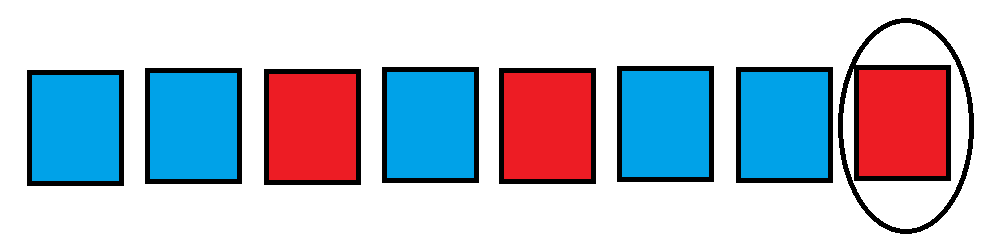
\includegraphics[width=\textwidth]{./tasks/07.png}
W powyższym przykładzie niebieskie kwadraty to nasze walizki, a czerwone to bagaże jakiejś rodziny z \(n_3\)\\
Ostatni bagaż jest ustalony, więc ustawień dla których \(X_{3j}=1\) jest \(\binom{7}{2}\), a wszystkich jest \(\binom{8}{3}\), stąd \(P(X_{3j})=\frac{\binom{7}{2}}{\binom{8}{3}}\)\\
Ogólniej dla każdej rodziny z \(n_i\) mamy \(P(X_{ij})=\frac{\binom{5+i-1}{i-1}}{\binom{5+i}{i}}\)\\
Liczymy wartość oczekiwaną jak zawsze:\\
\[E(X)=E(\sum_i \sum_j X_{ij})=\sum_i \sum_jE(X_{ij})=\sum_{i=1}^4 n_i\cdot \frac{\binom{5+i-1}{i-1}}{\binom{5+i}{i}}\]
Teraz możemy uprościć \(\frac{\binom{5+i-1}{i-1}}{\binom{5+i}{i}}\) do \(\frac{i}{i+5}\).\\
Zapisujemy mianownik jako \(\frac{i+5}{i} \binom{5+i-1}{i-1}\), dwumian się skróci, więc dostaniemy:
\subsection*{Odpowiedź}
\[E(X)=\sum_{i=1}^4 n_i \cdot \frac{i}{i+5}\]

\section{Zadanie 8 (Oskar Prusik)}
Niech \( a, b \) będą liczbami rzeczywistymi. Jakie warunki muszą spełniać \( a \) i \( b \), żeby istniała zmienna losowa, która ma wartość oczekiwaną równą \( a \) i wariancję równą \( b \)?  
W przypadku, gdy taka zmienna losowa istnieje, podaj ją.

\subsection*{Rozwiązanie}
Oczywistym jest, że wariancja jest nieujemna, co nakłada nam juz warunek: \[b \geq 0\]

Teraz znajdujemy przykład zmiennej losowej dla tylko tego jednego warunku. Niech zmienna losowa \(X\) ma rozkład:
\[
P(X = a + \sqrt{b}) = \frac{1}{2}, \quad P(X = a - \sqrt{b}) = \frac{1}{2}
\]
gdzie \(a \in \mathbb{R}\), \(b \geq 0\).


Korzystając z definicji wartości oczekiwanej dla zmiennej dyskretnej:
\[
E[X] = \sum x_i \cdot p_i = \frac{1}{2} \cdot (a + \sqrt{b}) + \frac{1}{2} \cdot (a - \sqrt{b})
\]
\[
= \frac{1}{2}a + \frac{1}{2}\sqrt{b} + \frac{1}{2}a - \frac{1}{2}\sqrt{b} = a
\]


\[
E[X^2] = \frac{1}{2} \cdot (a + \sqrt{b})^2 + \frac{1}{2} \cdot (a - \sqrt{b})^2
\]
\[
= \frac{1}{2} \cdot (a^2 + 2a\sqrt{b} + b) + \frac{1}{2} \cdot (a^2 - 2a\sqrt{b} + b)
\]
\[
= \frac{1}{2}a^2 + a\sqrt{b} + \frac{1}{2}b + \frac{1}{2}a^2 - a\sqrt{b} + \frac{1}{2}b
\]
\[
= a^2 + b
\]


Korzystając ze wzoru \(\mathrm{Var}(X) = E[X^2] - (E[X])^2\):
\[
\mathrm{Var}(X) = (a^2 + b) - a^2 = b
\]


\subsection*{Odpowiedź}
\[
\boxed{\text{Dla dowolnych \(a \in \mathbb{R}\) i \(b \geq 0\) istnieje zmienna losowa o podanej wartości oczekiwanej i wariancji.}}
\]

\section{Zadanie 9}
Podaj przykład zmiennej losowej, która ma skończoną wartość oczekiwaną,
i nieograniczoną wariancję.

\subsection*{Rozwiązanie}
W tym zadaniu chcemy znaleźć zbieżny szereg, który podniesiony do kwadratu jest rozbieżny. \\
Rozważmy następujący eksperyment: Losujemy liczbę ze zbioru liczb naturalnych.
Prawdopodobieństwo wylosowania liczby \(k\) jest równe \(\frac{C}{k^3}\).
\[ P(X=k) = \frac{C}{k^3} \]
\(C\) to tak dobrana stała żeby suma prawdopodobieństw wynosiła \(1\),
dokładniej \(C \approx 0,83\), ale to nas nie interesuje.

Zdefiniujmy zmienną losową \(X\) przyjmującą wartość wylosowanej liczby.

Z definicji wartości oczekiwanej: \\
\(E[X] = (1 \cdot P(X=1)) + (2 \cdot P(X=2)) + (3 \cdot P(X=3)) + \cdots\) \\
\(E[X] = (1 \cdot \frac{C}{1^3}) + (2 \cdot \frac{C}{2^3}) + (3 \cdot \frac{C}{3^3}) + \cdots\) \\
\(E[X] = C \cdot (\frac{1}{1^2} + \frac{1}{2^2} + \frac{1}{3^2} + \frac{1}{4^2} + \cdots)\)\\
a to z wielce znanego faktu jest skończone. OK.

To teraz wariancja:
z definicji \(Var(X) = E[X^2] - E[X]^2\). policzmy na początku \(E[x^2]\)\\
\(E[X^2] = (1^2 \cdot P(X=1)) + (2^2 \cdot P(X=2)) + (3^2 \cdot P(X=3)) + \cdots\) \\
\(E[X^2] = (1^2 \cdot \frac{C}{1^3}) + (2^2 \cdot \frac{C}{2^3}) + (3^2 \cdot \frac{C}{3^3}) + \cdots\) \\
\(E[X^2] = C \cdot (\frac{1}{1} + \frac{1}{2} + \frac{1}{3} + \frac{1}{4} + \cdots)\)\\
co ciekawe znowu otrzymaliśmy znany szereg, tym razem nieskończony.
Skoro \(E[X^2]\) jest nieskończone, a \(E[X]\) skończone, to \(E[X^2] - E[X]^2\) (czyli wariancja) jest nieskończona.

\subsection*{Odpowiedź}
\[
	\boxed{\text{Jest taki przykład, jak najbardziej, pokazany w rozwiązaniu}}
\]

\section{Zadanie 10}
Niech \(X\) będzie liczbą naturalną wylosowaną w sposób jednostajny z przedziału \([1, n]\),
a \(Y\) liczbą całkowitą wylosowaną w sposób jednostajny z przedziału \([-k, k]\).
Wyznaczyć \(\variance{X}\) oraz \(\variance{Y}\).

\subsection*{Rozwiązanie}
\begin{enumerate}

	\item \textbf{Wariancja zmiennej} \(X\), gdzie \(X\) jest wylosowane jednostajnie z przedziału \([1, n]\):

	      \[
		      \begin{aligned}
			      \ev{X}^2
			       & = \left( \frac{1 + 2 + \dots + n}{n} \right)^2
			      = \left( \frac{n + 1}{2} \right)^2,                               \\[6pt]
			      \ev{X^2}
			       & = \frac{1^2 + 2^2 + \dots + n^2}{n}
			      = \frac{(n + 1)(2n + 1)}{6},                                      \\[6pt]
			      \variance{X}
			       & = \ev{X^2} - \ev{X}^2                                          \\[3pt]
			       & = \frac{(n + 1)(2n + 1)}{6} - \left( \frac{n + 1}{2} \right)^2 \\[3pt]
			       & = \boxed{\frac{n^2 - 1}{12}}.
		      \end{aligned}
	      \]

	\item \textbf{Wariancja zmiennej} \(Y\), gdzie \(Y\) jest wylosowane jednostajnie z przedziału \([-k, k]\):

	      \[
		      \begin{aligned}
			      \ev{Y}
			       & = \frac{-k + (-k+1) + \dots + (k-1) + k}{2k+1}
			      = 0,                                              \\[6pt]
			      \ev{Y^2}
			       & = \frac{(-k)^2 + \dots + k^2}{2k+1}
			      = \frac{1}{2k+1}\sum_{n=-k}^{k} n^2               \\[3pt]
			       & = \frac{2}{2k+1}\sum_{n=1}^{k} n^2
			      = \frac{2}{2k+1} \cdot \frac{k(k+1)(2k+1)}{6}
			      = \frac{k(k+1)}{3},                               \\[6pt]
			      \variance{Y}
			       & = \ev{Y^2} - \ev{Y}^2
			      = \boxed{\frac{k(k+1)}{3}}.
		      \end{aligned}
	      \]

\end{enumerate}

\section{Zadanie 11}
Udowodnij, że jeśli \(\Var X = 0\), to istnieje \(a\)
takie, że \(P(X=a)=1\)

\subsection*{Rozwiązanie}
Skorzystamy z zadania 4. z pierwszego zestawu - dla ciągu zdarzeń
\(\{A_n\}\), jeśli \(\forall_{i\in\mathbb{N}} P(A_i) = 1\), to
\(P(\bigcap_{i\in\mathbb{N}} A_i) = 1\)

Niech \(a = E[X]\) (wartość oczekiwana istnieje, bo wariancja istnieje)

\subsubsection*{Lemat}
\[\forall \varepsilon > 0: P(|X-a| > \varepsilon) = 0\]

Zauważmy:
\[\Var X \geqslant
	\varepsilon^2 \cdot P(|X-a| > \varepsilon)\]
Wariancja jest sumą (całką) kwadratów odchyleń przyjmowanych wartości
od wartości oczekiwanej. Uwzględniając tylko te elementy, które nie
należą do zbioru \([a-\varepsilon, a+\varepsilon]\), dostajemy dolne
ograniczenie na wariancję.

Wiedząc że wariancja wynosi 0, to prawdopodobieństwo także musi być
zerowe. \(\quad\square\)

Przekształcając:
\[\forall \varepsilon > 0: P(|X-a| \leqslant \varepsilon) = 1\]
\[\forall \varepsilon > 0: P(X \in [a-\varepsilon, a+\varepsilon]) = 1\]

Podstawiając dla
\(\varepsilon = 1, \frac1{2}, \frac1{3}, \frac1{4}, \ldots\)
\[\forall_{n\in\mathbb{N_+}}
	P\left(X\in\left[a-\frac1{n}, a+\frac1{n}\right]\right) = 1\]
Teraz korzystając z zadania 1/4:
\[P(X\in\{a\}) = 1\quad\square\]

\section{Zadanie 12}
Czy jeśli dla dwóch zmiennych losowych X, Y mamy Cov(X, Y ) = 0 to
X, Y są niezależne?

\subsection*{Rozwiązanie}
Nie jest tak, można łatwo znaleźć kontrprzykład. Załóżmy, że z równym prawdopodobieństwem losujemy jedną z liczb \(\{-1,0,1\}\). Wówczas niech X - zmienna losowa oznaczająca wylosowaną liczbę. Zauważmy, że \(E[X] = (-1)\cdot P(X=-1) + 1\cdot P(X=1) + 0\cdot P(X = 0)= \frac{1}{3}\cdot (-1) + \frac{1}{3} \cdot 1 = 0\). Analogicznie \(E[X^3] = 0\). Teraz niech zmienna losowa Y = \(X^2\) oznacza kwadrat wylosowanej liczby. Wtedy \(E[Y] = \frac{1}{3}\cdot 1^2 + \frac{1}{3} \cdot (-1)^2  + \frac{1}{3} \cdot 0^2= \frac{2}{3}\). Oczywiście zmienne X i Y nie są niezależne, np. \(P(X=1 \And Y=0) = 0 \neq \frac{1}{9} =  P(X = 1) \cdot P(Y = 0)\), a mimo to:
\[
	Cov(X,Y) = E[XY] - E[X]E[Y] = E[X^3] - 0 = 0
\]


\subsection*{Odpowiedź}
\[
	\boxed{\text{Nie}}
\]


\section{Zadanie 13}
Udowonij że każdy graf zawiera podgraf dwudzielny, który ma co najmniej połowę kraedzi oryginalnego grafu. Wskazówka: Pamiętaj, że graf dwudzielny to innymi słowy, graf dwukolorowalny.

W następnyh zadaniach pomocna może się okazać następująca trywialna obserwacja. Jeśli wartość pewnej zmiennej losowej $X$ wynosi $x$, to $P(X \geq x) > 0$ (podobnie $P(X \leq x) > 0$) 

\subsection*{Rozwiązanie}

E(X) - oczekiwana liczba krawędzi.

$X_i$ - i-ta krawędź w grafie dwudzielnym.

Zaczynamy od pokolorawnia wierzchołków grafu na 2 kolory z równym prawdopodobieńswem $\frac{1}{2}$. Dla każdej krawędzi, sprawdzamy wierzchołki, na których się kończy. Jeśli są takie samę, to taką krawędź usuwamy z grafu, a jeśli inne to zostawiamy. Prawdopodobieńswo, że zostawiamy, jakąś kradź to $2*\frac{1}{4}$, czyli $\frac{1}{2}$. Łatwo, to zauważyć, bo są 2 przypadki, kiedy zostawiamy: pierwszy kolor + drugi oraz drugi + pierwszy. Pozostałe pierwszy + pierwszy i drugi + drugi są złe zgodnie z wcześniejszą definicją.


\[
    E(X) = E(\sum_{i = 1}^{m} E_i) = \sum_{i = 1}^{m} E(X_i) = \sum_{i = 1}^{m} P(X_i) = \sum_{i = 1}^{m} \frac{1}{2} = m * \frac{1}{2} = \frac{m}{2}
\]

Skoro wiemu, że wartość oczekiwana liczby krawędzi to $\frac{m}{2}$ to wiemy, że prawdopodobieńswo istenienia grafu o $\frac{m}{2}$ krawędziach jest większe od zera. To natomaist oznacza, że  graf wyjściowy musi mieć podgraf, któy jest dwudzielny i ma co najmniej $\frac{m}{2}$ krawędzi.
\section{Zadanie 14}

Udowodnij, że dla każdego dodatniego $n$ istnieje turniej (graf skierowany
pełny) na $n$ wierzchołkach, który ma co najmniej $\frac{n!}{2^{n-1}}$ ścieżek Hamiltona.

\subsection*{Rozwiązanie}

Rozważmy nieskierowany graf pełny na $n$ wierzchołkach. Będziemy kierować wszystkie jego krawędzie z równym prawpodpodobieństwem dla dwóch stron. Policzmy wartość oczekiwaną liczby ścieżek Hamiltona dla naszego grafu. Z liniowośći wartości oczekiwanej możemy rozbić ją na sumę wartości oczekiwanych indykatorów czy dana permutacja wierzchołków jest ścieżką Hamiltona. Permutacji jest $n!$, dla każdej z nich wartość oczekiwana jest równa prawdopodobieństwu i wynosi $\frac{1}{2^{n-1}}$ (mamy $n-1$ krawędzi, tylko jedno ze skierowań daje ścieżkę Hamiltona). Po zsumowaniu dostajemy wartość oczekiwaną ścieżek Hamiltona w grafie $\frac{n!}{2^{n-1}}$, z czego na mocy uwagi z zadania 13 wynika, że prawdopodbieństwo tego, że graf ma conajmniej tyle ścieżek Hamiltona jest większe od zera, czyli musi istnieć takie skierowanie które spełnia warunki zadania. 
\section{Zadanie 15}
\autor{Filip Manijak}
Udowodnij, że każdy graf dwudzielny z $m$ krawędziami zawiera podgraf na
co najmniej $\frac{3}{4} m^{\frac{2}{3}}$ krawędziach, który nie zawiera cyklu na czterech
wierzchołkach $C_4$ jako podgrafu.

\vspace{0.5em}

\textbf{Uwaga:} Wystarczy pokazać ograniczenie $\frac{1}{2} m^{\frac{2}{3}}$.

\vspace{0.5em}

\textbf{Wskazówka:} Grafy można losować. Jednym ze sposobów jest ustalenie
pewnego parametru $p$ i dla każdej pary wierzchołków niezależne wylosowanie
tego, czy łączy je krawędź, czy nie, z prawdopodobieństwem $p$. Jeśli
losowany graf nie działa, to może należy go zmodyfikować po wylosowaniu?


\subsection*{Rozwiązanie}
Najpierw pokażę lemat:
\subsection{Lemat: Liczba cykli w grafie dwudzielnym to max $\frac{|E|^2}{4}$}
Dlaczego? Bo par rozłącznych krawędzi jest $\frac{|E||E-1|}{2}$. Zauważmy, że każda para rozłącznych krawędzi występuje razem w max. 1 $C_4$. Oszacowanie jeszcze musimy podzielić na 2, bo każdy cykl zliczamy 2 razy. 
\subsection{Główny pomysł}
Będziemy losować graf (każdą krawędź z pwdp. $p$) i zauważymy że liczba cykli jest całkiem mała. W podgrafie naszego grafu dwudzielnego, powstałym w taki sposób że każda krawędź występuje w nim z prawdopodobieństwem $p$ jest w wartości oczekiwanej:
\begin{itemize}
    \item $pm$ krawędzi (liniowość wartości oczekiwanej)
    \item $p^4num\_C_4$ $C_4$ (wszystkie 4 krawędzie muszą zostać przeniesione)
\end{itemize}
Zauważmy, że wystarczy usunąć tyle krawędzi co cykli, żeby żadnych cykli nie było. Czyli, stwórzmy nowy sposób losowania grafu: Losujemy każdą krawędź z prawdopodobieństwem $p$, ale jeśli krawędź ta tworzy $C_4$ to jej nie bierzemy. Teraz policzmy wartość oczekiwaną:
$$E[E(H)] = pm - p^4\frac{m^2}{4}$$
Co po podstawieniu $p = m^{-1/3}$ daje:
$$E[E(H)] = \frac{3}{4} m^\frac{2}{3}$$
Z trywialnej obserwacji$^{TM}$ koniec dowodu.




\chapter{Zestaw 3 -- Miara i całka}
\chaptermark{Zestaw 3}
\graphicspath{{chapters/zestaw-03/}}
\section{Zadanie 1}
Udowodnij, że liczba elementów skończonej algebry (czyli też \(\sigma\)-algebry) jest potęgą dwójki.

\subsection*{Rozwiązanie}
(Tak jak w zadaniu 2) Rozważamy atomy w danej \(\sigma\)-algebrze. Niech n - liczba atomów, zgodnie z warunkami jakie musi spełniać \(\sigma\)-algebra suma każdego podzbioru atomów musi należeć do tej algebry. Liczba podzbiorów zbioru \(n\)-elementowego to \(2^{n}\) zatem liczba elementów skończonej \(\sigma\)-algebry musi być potęgą dwójki CKD

\section{Zadanie 2}
Czy istnieje nieskończona przeliczalna \(\sigma\)-algebra?

\subsection*{Rozwiązanie}
Nie istnieje nieskończona przeliczalna \(\sigma\)-algebra. Pokazmy sobie to na atomach.
Atom w \(\sigma\)-algebrze to taki zbiór \(A\) należący do tej \(\sigma\)-algebry, że dla dowolnego podzbioru \(B \subseteq A\) zachodzi \(B = \emptyset\) lub \(B = A\). Oznacza to, że atom nie może być podzielony na mniejsze zbiory należące do tej samej \(\sigma\)-algebry.

Widzimy ze jesli mamy skonczoną liczbę atomów to \(\sigma\)-algebra jest skończona, bo każdy zbiór w \(\sigma\)-algebrze można przedstawić jako sumę atomów. Czyli mamy \(2^n\) podzbiorów dla \(n\) atomów.

To teraz załózmy ze mamy nieskończenie i przeliczalnie wiele atomów. I zastanówmy się ile mamy podzbiorów.
No mamy ich \(|\mathbb{P}(A)| = 2^A = 2^{\aleph_0}\) poniewaz rozwazamy \(A\) które jest nieskończone i przeliczalne.
A z MFI wiemy ze \(2^{\aleph_0}\) jest nieprzeliczalne bo jest równe na moc continuum.

\subsection*{Odpowiedź}
\[
	\boxed{\text{Nie}}
\]

\section{Zadanie 3}
Niech $B\subseteq\Omega$ i niech $\sum_B = \{ A\subseteq\Omega :B\subseteq A$ lub $B\cap A = \emptyset\}$. Udowodnij, że $\sum_B$  jest $\sigma$-algebrą.
\subsection*{Rozwiązanie}
Przejdźmy kolejno po poszczególnych przypadkach.
\begin{enumerate}
\item Zbiór $\emptyset\in \sum_B$ ponieważ $B\cap\emptyset=\emptyset$. Zbiór $\Omega\in \sum_B$ ponieważ $B\subseteq\Omega$.
\item Weźmy $E\in\sum_B$ i zauważmy że jeśli $E$ spełnia warunek, że $E\cap B = \emptyset$ to $B\subseteq\Omega\setminus E$. Jeśli zaś zachodzi, że $B\subseteq E$ to zachodzi $(\Omega\setminus E)\cap B = \emptyset$.
\item Jeżeli $\exists_i$ takie że $E_i$ spełnia warunek $B\subseteq E_i$ to wtedy $B\subseteq \bigcup_{i=1}^n E_i$ zatem $\bigcup_{i=1}^n E_i \in \sum_B$. Jeżeli taki zaś nie istnieje to dla każdego $i$ zachodzi $E_i\cap B=\emptyset$ zatem $\bigcup_{i=1}^n E_i \cap B=\emptyset$ czyli $\bigcup_{i=1}^n E_i\in\sum_B$.
\item analogicznie jak 3 podpunkt bo nie korzystamy tam z tego że suma jest skończona
\end{enumerate}

\section{Zadanie 4}
Niech $\Sigma_{\aleph_{0}}$ będzie rodziną wszystkich podzbiorów $\Omega$,
które albo są co najwyżej przeliczalne, albo ich dopełnienia są co najwyżej przeliczalne. Udowodnij,
że $\Sigma_{\aleph_{0}}$ jest $\sigma$-algebrą.

\subsection*{Rozwiązanie}
Sprawdzamy warunki:
\begin{enumerate}
    \item $\emptyset, \Omega \in \Sigma_{\aleph_{0}}$
        \begin{quote}
            $\emptyset$ - jest co najwyżej przeliczalny, z tego mamy $\emptyset \in \Sigma_{\aleph_{0}}$.

            Dla $\Omega$ mamy, że $\Omega / \Omega = \emptyset$ który jest przeliczalny, stąd $\Omega \in \Sigma_{\aleph_{0}}$.
        \end{quote}
    \item Jeśli $E \in \Sigma_{\aleph_{0}}$ to $\Omega/E \in \Sigma_{\aleph_{0}}$
        \begin{quote}
            Z tego, że $E \in \Sigma_{\aleph_{0}}$ mamy, $E$ - co najwyżej przeliczalny lub $\Omega/E$ - co najwyżej przeliczalny.
            \begin{itemize}
                \item $E$ - co najwyżej przeliczalny, wtedy $\Omega/E \in \Sigma_{\aleph_{0}}$, bo $\Omega/(\Omega/E) = E$ - co najwyżej przeliczalny.
                \item $\Omega/E$ - co najwyżej przeliczalny, to $\Omega/E \in \Sigma_{\aleph_{0}}$, bo $\Omega/E$ - co najwyżej przeliczalny.
            \end{itemize}
        \end{quote}
    \item Jeśli $E_{1},\dots,E_{n} \in \Sigma_{\aleph_{0}}$, to $\bigcup^{n}_{i=1}E_{i}\in\Sigma_{\aleph_{0}}$
        \begin{quote}
            \begin{itemize}
                \item Jeśli $\forall_{i}E_{i}$ - co najwyżej przeliczalny, to $\bigcup^{n}_{i=1}E_{i}$ też co najwyżej przeliczalna, co znaczy, że $\bigcup^{n}_{i=1}E_{i}\in\Sigma_{\aleph_{0}}$.
                \item Niech $E_{x}$ nie będzie co najwyżej przeliczalny, to $\Omega/E_{x}$ jest co najwyżej przeliczalny. $\Omega/\bigcup^{n}_{i=1}E_{i} = \bigcap^{n}_{i=1}\Omega/E_{i} \subset \Omega/E_{x} \implies \bigcap^{n}_{i=1}\Omega/E_{i}$ co najwyżej przeliczalny, stąd $\bigcup^{n}_{i=1}E_{i}\in\Sigma_{\aleph_{0}}$.
            \end{itemize}
        \end{quote}
    \item Jeśli $E_{1},\dots,E_{\infty} \in \Sigma_{\aleph_{0}}$, to $\bigcup^{\infty}_{i=1}E_{i}\in\Sigma_{\aleph_{0}}$
        \begin{quote}
            \begin{itemize}
                \item Jeśli $\forall_{i}E_{i}$ - co najwyżej przeliczalny, to $\bigcup^{\infty}_{i=1}E_{i}$ też co najwyżej przeliczalna, co znaczy, że $\bigcup^{\infty}_{i=1}E_{i}\in\Sigma_{\aleph_{0}}$.
                \item Niech $E_{x}$ nie będzie co najwyżej przeliczalny, to $\Omega/E_{x}$ jest co najwyżej przeliczalny. $\Omega/\bigcup^{\infty}_{i=1}E_{i} = \bigcap^{\infty}_{i=1}\Omega/E_{i} \subset \Omega/E_{x} \implies \bigcap^{\infty}_{i=1}\Omega/E_{i}$ co najwyżej przeliczalny, stąd $\bigcup^{\infty}_{i=1}E_{i}\in\Sigma_{\aleph_{0}}$.
            \end{itemize}
        \end{quote}
\end{enumerate}

$
\boxed{\text{}}
$

\section{Zadanie 5 (Kacper Orszulak)}
Udowodnij, że jeśli $\left\{ \Sigma_\alpha : \alpha \in I \right\}$ jest rodziną $\sigma$-algebr na jakimś ustalonym zbiorze $\Omega$ (dla dowolnego zbioru indeksów $I$), to $\bigcap_{\alpha \in I} \Sigma_\alpha$ też jest $\sigma$-algebrą.

\subsection*{Rozwiązanie}
Niech $\Sigma := \bigcap_{\alpha \in I} \Sigma_\alpha$. Po kolei sprawdzamy warunki.
\begin{enumerate}
    \item \textit{$\emptyset, \Omega \in \Sigma$}
        \begin{quote}
        $\forall_{\alpha \in I} \; \emptyset, \Omega \in \Sigma_\alpha \implies \emptyset, \Omega \in \bigcap_{\alpha \in I} \Sigma_\alpha = \Sigma$
        \end{quote}
    \item \textit{Jeśli $E \in \Sigma$ to $\Omega/E \in \Sigma$}
        \begin{quote}
        Niech $E \in \Sigma$. Wtedy $\forall_{\alpha \in I} \; E \in \Sigma_\alpha \iff \Omega / E \in \Sigma_\alpha$.

        Dostajemy zatem $\Omega/E \in \bigcap_{\alpha \in I} \Sigma_\alpha = \Sigma$.
        \end{quote}
    \item \textit{Jeśli $E_1, ..., E_n \in \Sigma$, to $\bigcup_{i=1}^n E_i \in \Sigma$}
        \begin{quote}
        Niech $E_1, ..., E_n \in \Sigma$. Wtedy $\forall_{\alpha \in I} \; E_1, ..., E_n \in \Sigma_\alpha \implies \bigcup_{i=1}^n E_i \in \Sigma_\alpha$.

        Dostajemy zatem $\bigcup_{i=1}^n E_i \in \bigcap_{\alpha \in I} \Sigma_\alpha = \Sigma$.
        \end{quote}
    \item \textit{Jeśli $E_1, E_2, ... \in \Sigma$, to $\bigcup_{i=1}^\infty E_i \in \Sigma$}
        \begin{quote}
        Niech $E_1, E_2, ... \in \Sigma$. Wtedy $\forall_{\alpha \in I} \; E_1, E_2, ... \in \Sigma_\alpha \implies \bigcup_{i=1}^\infty E_i \in \Sigma_\alpha$.

        Dostajemy zatem $\bigcup_{i=1}^\infty E_i \in \bigcap_{\alpha \in I} \Sigma_\alpha = \Sigma$.
        \end{quote}
\end{enumerate}
$\square$

\section{Zadanie 6}
\autor{Mateusz Wojaczek}
Udowodnij, że każdy zbiór otwarty $B \subseteq \mathbb{R}$ jest co najwyżej przeliczalną sumą przedziałów otwartych. Dodatkowo pokaż, że $\mathcal{A}_0$ jest zamknięty na branie dowolnych sum (także nieskończonych).

\subsection*{Rozwiązanie}
Niech $B \subseteq \mathbb{R}$ będzie zbiorem otwartym. Z definicji zbioru otwartego:

\[
\forall x \in B \;\; \exists \varepsilon > 0 \text{ takie, że } (x-\varepsilon, x+\varepsilon) \subseteq B.
\]

Z MFI wiadomo, że w każdym przedziale otwartym $(x-\varepsilon, x+\varepsilon)$ istnieje liczba wymierna. \\
Liczb wymiernych jest przeliczalne wiele. 
$\mathbb{Q}$ jest przeliczalne.

Dla każdej liczby wymiernej $q \in \mathbb{Q}$ zdefiniujmy:

\[
B_q = \{ x \in B \mid q \in (x-\varepsilon_x, x+\varepsilon_x) \text{ dla pewnego } \varepsilon_x > 0 \}.
\]

Wtedy każdy punkt $x \in B$ należy do jakiegoś $B_q$, ponieważ w przedziale $(x-\varepsilon_x, x+\varepsilon_x) \subseteq B$ znajduje się liczba wymierna $q$. Zatem:

\[
B = \bigcup_{q \in \mathbb{Q}} B_q.
\]

Każdy $B_q$ jest sumą przedziałów otwartych zawierających $q$, a ponieważ $\mathbb{Q}$ jest przeliczalne, $B$ jest sumą przeliczalną przedziałów otwartych.

\medskip
\textbf{Dowód zamknięcia $\mathcal{A}_0$ na dowolne sumy:}

Niech $\{U_i\}_{i \in I} \subseteq \mathcal{A}_0$ będzie dowolną rodziną zbiorów otwartych.
Rozważmy sumę:

\[
U = \bigcup_{i \in I} U_i.
\]

Niech $x \in U$. Wówczas istnieje $i_0 \in I$ takie, że $x \in U_{i_0}$. Ponieważ $U_{i_0}$ jest otwarty, istnieje $\varepsilon > 0$ takie, że $(x-\varepsilon, x+\varepsilon) \subseteq U_{i_0} \subseteq U$. Zatem każdy punkt $x \in U$ należy do pewnego przedziału zawartego w $U$, co pokazuje, że $U$ jest otwarty.  

Zatem $U \in \mathcal{A}_0$, co dowodzi, że $\mathcal{A}_0$ jest zamknięty na dowolne sumy (w tym nieskończone).

\subsection*{Odpowiedź}
\[
\boxed{\text{CKD}}
\]

\section{Zadanie 7}
\autor{Aleksander Wieczorek}
Udowodnij, że \(A_0\) nie jest zamknęty na branie nieskończonych przecięć.
\subsection*{Rozwiązanie}
Zbiór zamknięty na branie przecięć to taki, że dla każdego podzbioru elementów tego zbioru ich przecięcie również należy do tego zbioru.\\
Żeby dostać tezę wystarczy pokazać, że istnieje nieskończony podzbiór przedziałów otwartych, których przecięcie to przedział, który jest domknięty z którejś strony.\\
Możemy wziąć np.
\[\bigcap_{n=1}^\infty \left(-\frac{1}{n},\frac{1}{n}\right)=\{0\}=[0,0] \notin A_0\]
Zbiór \(A_0\) nie jest zamknięty na przecięcia, bo dostaliśmy element spoza niego.\\
jeśli chcemy wziąć zbiór inny niż singleton możemy wziąć np.
\[\bigcap_{n=1}^\infty \left(-\frac{1}{n},1+\frac{1}{n}\right)=[0,1]  \notin A_0\]
\section{Zadanie 8}
Niech $A_{\infty} = \{(-\infty, a]: a \in R\}$ i niech $U \in A_0$. Udowodnij, że ażda $\sigma$-algebra zawierająca $A_{\infty}$ zawiera $U$. Innymi słowy pokazujemy, że $A_0 \subseteq \sigma (A_{\infty})$, a co za tym idzie $\sigma (A_0) \subseteq \sigma (A_{\infty})$. Podobnie pokaż, że $\sigma (A_0) \supseteq \sigma (A_{\infty})$

\subsection*{Rozwiązanie}
Pokażemy, że element zbiór otwarty(element $A_0$), może być generowany przez elementy z $A_{\infty}$.

Zaczneimy od obserwacji, że poniważ każdy zbiór otwarty jest sumą przeliczalnej liczby przedziałów otwartych, wieć wystarczy nam pokazać, że dowolny przedział $(a, b)$ może być generowany przez $A_{\infty}$.

Weźmy nieskończoną rodzinę $B$, gdzie $B_n$ to $(-\infty, b - \frac{1}{n}]$. Nieskończoną sumą tej rodziny. $U_B = (-\infty, b)$. Teraz weźmy dopełnienie i otrzymamy: $[b, +\infty)$. Następnie możemy to szumować z $(-\infty, a]$ i na koniec wziąść dopełnienie tego. Otrzymany wynik to $(a, b)$. To natomiast oznacza, że $A_{\infty}$, generuję każdy przedział. 

Żeby pokazać zawieranie w drugą stronę wystarczy wziąść dopełnienie od przedziału otwartego $(a, +\infty)$, co daje $(-\infty, b]$.

Z tych faktu wychodzi, ze $\sigma (A_0) = \sigma (A_{\infty})$.

\section{Zadanie 9}
 Niech $\nu : \mathcal{B}(\mathbb{R}) \to \{0,1\}$ będzie zdefiniowana następująco. 
Dla $B \in \mathcal{B}(\mathbb{R})$ mamy $\nu(B) = 1$ wtedy i tylko wtedy, gdy istnieje $\varepsilon > 0$ taki, że $(0,\varepsilon) \subseteq B$. 
Czy funkcja $\nu$ jest skończenie addytywna? 
Jeśli tak, to czy jest przeliczalnie addytywna?
\subsection*{Rozwiązanie}

Niech $E_1 = \mathbb{Q} \cap (0,1) \in \mathcal{B}(\mathbb{R})$ i $E_2 = (0,1) \setminus \mathbb{Q} \in \mathcal{B}(\mathbb{R})$.

$\nu(E_1) = \nu({E_2}) = 0$, a $\nu(E_1 \cup E_2) = \nu( (0,1) ) = 1 \neq \nu(E_1) + \nu(E_2) = 0$.

\subsection*{Odpowiedź}
\[
\boxed{\text{Nie jest skończenie addytywna}}
\]

\section{Zadanie 10}
\autor{Filip Manijak}
Niech \((\Omega, \Sigma)\) i \((\Omega', \Sigma')\) będą przestrzeniami mierzalnymi oraz \(\sigma(\mathcal{G}) = \Sigma'\) dla pewnego \(\mathcal{G} \subseteq \mathcal{P}(\Omega')\) (innymi słowy \(\Sigma'\) jest generowana przez \(\mathcal{G}\)). Udowodnij, że \(f : \Omega \to \Omega'\) jest mierzalna wtedy i tylko wtedy, gdy \(f^{-1}(G) \in \Sigma\) dla każdego \(G \in \mathcal{G}\).

\subsection*{Rozwiązanie}
Sprawadza się to, do udowodnienia że:
\[f^{-1}(G) \in \Sigma \iff f^{-1}(\sigma(G)) \in \Sigma\]
\subsection{\(\Leftarrow\)}
Triv, bo \(G \subset \sigma(G)\)
\subsection{\(\implies\)}
Tu plan jest taki, że pokażemy że wszystkie zbiory o mierzalnym przeciwobrazie są \(\sigma\)-algebrą (oznaczmy ją \(M\) jak mierzalne). Wiemy jednak, że \(G\) należy do tej sigma algebry, a to oznacza że \(\sigma(G) \subset M\) bo \(\sigma(G)\) to przecięcie \(M\) z czymś tam (nie interesuje nas czym). No to teraz ta trudniejsza cześć, pokazanie tego
\subsection{Dowód że \(\{X: f^{-1}(X) \in \Sigma\} = M\) jest \(\sigma\)-algebrą}
Sprawdzamy własności:
\begin{itemize}
	\item \(\Omega' \in M\), tak ponieważ \(f^{-1}(\Omega') = \Omega \in \Sigma\)
	\item \(A \in M \implies \Omega'/A \in M\) też, ponieważ \(f^{-1}(\Omega'/A) = f^{-1}(\Omega')/f^{-1}(A)\) co już jest w \(M\) bo \(\Sigma\) to algebra
	\item Suma przeciwobrazów podobnie się przenosi, więc ten sam argument.
	\item Suma przeliczalnej ilości zachowuje się trywialnie tak samo.
\end{itemize}

\section{Zadanie 11}
Czy złożenie dwóch funkcji mierzalnych jest mierzalne?

\subsection*{Rozwiązanie}
Niech dane będą \((\Omega_1, \Sigma_1)\), \((\Omega_2, \Sigma_2)\), \((\Omega_3, \Sigma_3)\) oraz funkcje \(f: (\Omega_1, \Sigma_1) \xrightarrow{} (\Omega_2, \Sigma_2)\), \(g: (\Omega_2, \Sigma_2) \xrightarrow{} (\Omega_3, \Sigma_3)\), które są mierzalne.

Dla przypomnienia, funkcja \(h: (\Omega, \Sigma) \xrightarrow{} (\Omega', \Sigma')\) jest mierzalna wtw. gdy \(\forall_{E\in\Sigma'}  h^{-1}(E) \in \Sigma\).

Niech więc \(E \in \Sigma_3\). Z mierzalności \(g\) wiadomo, że \(g^{-1}(E) \in \Sigma_2\). Z tego i z mierzalności \(f\) wiadomo też, że \(f^{-1}(g^{-1}(E)) \in \Sigma_1\).

Pokazaliśmy, że dla każdego \(E \in \Sigma_3\) zachodzi \((g \circ f)^{-1}(E) \in \Sigma_1\), przez co \((g \circ f)\) jest mierzalna.

\subsection*{Odpowiedź}
\[
	\boxed{\text{Tak, złożenie dwóch funkcji mierzalnych jest mierzalne.}}
\]

\section{Zadanie 12}
Czy każda funkcja ciągła $f: \mathbb{R} \to \mathbb{R}$ jest mierzalna?

\subsection*{Rozwiązanie}
Tak, pokażemy, że każda taka funkcja jest $\mathcal{B}(\mathbb{R})$-mierzalna.
Niech $\mathcal{A}_0$ oznacza rodzinę wszystkich zbiorów otwartych w $\mathbb{R}$. Wiemy, że $\sigma(\mathcal{A}_0) = \mathcal{B}(\mathbb{R})$
Na podstawie definicji Cauchy'ego ciągłości funkcji $f$ mamy
\[
\forall A \in \mathcal{A}_0 \quad f^{-1}(A) \in \mathcal{A}_0,
\]
czyli przeciwobraz każdego zbioru otwartego jest również zbiorem otwartym.

Teraz wykorzystamy zadanie 10 z zestawu 3. Podstawiając tam:
\[
\Omega _1 = \Omega _2 = \mathbb{R};  \Sigma _1 = \Sigma _2 = \mathcal{B}(\mathbb{R}) ; \mathcal{G} = \mathcal{A}_0
\]
otrzymujemy, że f jest mierzalna.

\subsection*{Odpowiedź}
\[
\boxed{\text{Tak, w ujęciu borelowskim}}
\]

\section{Zadanie 13}
\autor{Oskar Prusik}
\textbf{Teza:} Niech $f, g : \mathbb{R} \to \mathbb{R}$ będą mierzalne. Czy ich suma również jest mierzalna?

\subsection*{Rozwiązanie}


Niech $\mathcal{G} = \{ (-\infty, c) : c \in \mathbb{R} \}$. 
Wiadomo, że $\sigma(\mathcal{G}) = \mathcal{B}(\mathbb{R})$.
(co łatwo wynika z warunków na $\sigma$-algebrę oraz faktu, że $\sigma(\mathcal{A}_0) = \mathcal{B}(\mathbb{R})$)

Zgodnie z zadaniem 10, aby wykazać mierzalność $f + g$, wystarczy sprawdzić, że dla każdego $G \in \mathcal{G}$:
\[
(f + g)^{-1}(G) \in \mathcal{B}(\mathbb{R}).
\]

Weźmy dowolne $c \in \mathbb{R}$ i rozważmy zbiór:
\[
A = \{ x \in \mathbb{R} : f(x) + g(x) < c \} = (f + g)^{-1}((-\infty, c)).
\]

Zauważmy, że:
\[
f(x) + g(x) < c \quad \iff \quad f(x) < c - g(x).
\]
Istnieje wtedy liczba wymierna $r \in \mathbb{Q}$ taka, że:
\[
f(x) < r < c - g(x).
\]
Zatem:
\[
A = \bigcup_{r \in \mathbb{Q}} \left( \{ x : f(x) < r \} \cap \{ x : g(x) < c - r \} \right).
\]

Ponieważ $f$ i $g$ są mierzalne, zbiory:
\[
\{ x : f(x) < r \} \in \mathcal{B}(\mathbb{R}), \quad \{ x : g(x) < c - r \} \in \mathcal{B}(\mathbb{R}).
\]
Przekrój dwóch zbiorów borelowskich jest borelowski, a przeliczalna suma zbiorów borelowskich jest borelowska. 
Zatem $A \in \mathcal{B}(\mathbb{R})$.

Wnioskujemy, że $(f + g)^{-1}((-\infty, c)) \in \mathcal{B}(\mathbb{R})$ dla każdego $c \in \mathbb{R}$, 
czyli warunek mierzalności jest spełniony na generatorze $\mathcal{G}$. 
Z zadania 10 wynika, że $f + g$ jest mierzalna.


\subsection*{Odpowiedź}
\[
\boxed{\text{Suma też jest mierzalna.}}
\]

\section[\nierozwiazane{Zadanie 14}]{Zadanie 14}

\brakrozwiazania

\section{Zadanie 15}

Udowodnij, że jeśli $f, g : \Omega \to \mathbb{C}$ są mierzalne, to
\[
\int_E (f + g) \, d\mu = \int_E f \, d\mu + \int_E g \, d\mu.
\]

\textbf{Wskazówka:}  

Najpierw udowodnij równość dla $f$ i $g$ będących funkcjami schodkowymi.  
Następnie skorzystaj z twierdzenia o aproksymacji funkcji mierzalnej funkcjami schodkowymi.  
Przejście od funkcji nieujemnych do funkcji rzeczywistych i zespolonych jest bardzo proste.

\subsection*{Rozwiązanie}
\textbf{Etap 1: Liniowość całki dla funkcji schodkowych}
\\

Niech $f, g : \Omega \to \mathbb{C}$ będą funkcjami schodkowymi, tzn.
\[
f = \sum_{i=1}^{n} a_i \chi_{A_i}, \qquad
g = \sum_{j=1}^{m} b_j \chi_{B_j},
\]
gdzie $A_i, B_j \subseteq \Omega$ są mierzalnymi i rozłącznymi zbiorami w obrębie $\Omega$, a $a_i, b_j \in \mathbb{C}$.

Wiemy, że
\[
(f+g)(x) = f(x) + g(x).
\]
Ponieważ $f(x) = a_i$ dla $x \in A_i$, a $g(x) = b_j$ dla $x \in B_j$, otrzymujemy:
\[
(f+g)(x) = a_i + b_j \quad \text{dla } x \in A_i \cap B_j.
\]

Zatem funkcja $f+g$ jest również schodkowa i można ją zapisać jako
\[
f + g = \sum_{i=1}^{n} \sum_{j=1}^{m} (a_i + b_j) \chi_{A_i \cap B_j}.
\]

Z definicji całki dla funkcji schodkowej mamy:
\[
\int_E (f+g)\, d\mu = \sum_{i=1}^{n} \sum_{j=1}^{m} (a_i + b_j) \, \mu(E \cap A_i \cap B_j).
\]

Rozdzielając sumę i korzystając z własności sum:
\[
\int_E (f+g)\, d\mu
= \sum_{i=1}^{n} \sum_{j=1}^{m} a_i \, \mu(E \cap A_i \cap B_j)
+ \sum_{i=1}^{n} \sum_{j=1}^{m} b_j \, \mu(E \cap A_i \cap B_j).
\]

Korzystając z rozłączności zbiorów $B_j$ i $A_i$, otrzymujemy:
\[
\sum_{j=1}^{m} \mu(E \cap A_i \cap B_j) = \mu(E \cap A_i), \qquad
\sum_{i=1}^{n} \mu(E \cap A_i \cap B_j) = \mu(E \cap B_j),
\]
czyli
\[
\int_E (f+g)\, d\mu = \sum_{i=1}^{n} a_i \, \mu(E \cap A_i) + \sum_{j=1}^{m} b_j \, \mu(E \cap B_j).
\]

Z definicji całki funkcji schodkowej mamy wprost:
\[
\int_E f \, d\mu = \sum_{i=1}^{n} a_i \, \mu(E \cap A_i), \qquad
\int_E g \, d\mu = \sum_{j=1}^{m} b_j \, \mu(E \cap B_j),
\]
więc wreszcie:
\[
\int_E (f+g)\, d\mu = \int_E f\, d\mu + \int_E g\, d\mu.
\]

\vspace{1em}

\textbf{Etap 2: Liniowość całki dla funkcji mierzalnych nieujemnych}
\\

Z twierdzenia o aproksymacji funkcji mierzalnej funkcjami schodkowymi, weźmy $S_1, \dots, S_n$ i $T_1, \dots, T_n$ takie, żeby
\[
\lim_{n \to \infty} S_n = f, \qquad \lim_{n \to \infty} T_n = g.
\]

Wtedy
\[
\lim_{n \to \infty} (S_n + T_n) = f+g.
\]

Z liniowości całki dla funkcji schodkowych otrzymujemy dla funkcji nieujemnych mierzalnych:
\[
\int_E (f+g) \, d\mu = \lim_{n \to \infty} \int_E (S_n + T_n) \, d\mu 
= \lim_{n \to \infty} \int_E S_n \, d\mu + \lim_{n \to \infty} \int_E T_n \, d\mu 
= \int_E f \, d\mu + \int_E g \, d\mu.
\]

\vspace{1em}

\textbf{Etap 3: Liniowość całki dla funkcji rzeczywistych}
\\

Rozbijmy
\[
f = f_+ - f_-, \qquad g = g_+ - g_-,
\]
gdzie
\[
f_+ = \max\{0,f\}, \quad f_- = -\min\{0,f\},
\]
analogicznie dla funkcji $g$.

Jako że $f_+, f_-, g_+, g_-$ są funkcjami mierzalnymi, nieujemnymi, zastosujemy w dowodzie wynik z Etapu 2:
\[
\begin{aligned}
\int_E (f+g) \, d\mu 
&= \int_E (f_+ - f_-) + (g_+ - g_-) \, d\mu \\
&= \int_E (f_+ + g_+) - (f_- + g_-) \, d\mu \\
&= \int_E (f_+ + g_+) \, d\mu - \int_E (f_- + g_-) \, d\mu \\
&= \int_E f_+ \, d\mu + \int_E g_+ \, d\mu - \int_E f_- \, d\mu - \int_E g_- \, d\mu \\
&= \int_E f \, d\mu + \int_E g \, d\mu.
\end{aligned}
\]

\vspace{1em}

\textbf{Etap 4: Liniowość całki dla funkcji zespolonych}
\\

Niech $f, g : \Omega \to \mathbb{C}$ będą funkcjami mierzalnymi.  
Rozbijamy je na części rzeczywistą i urojoną:
\[
f = \Re(f) + i \Im(f), \qquad g = \Re(g) + i \Im(g),
\]
gdzie $\Re(f), \Im(f), \Re(g), \Im(g)$ są funkcjami rzeczywistymi mierzalnymi.

Zastosowując liniowość całki dla funkcji rzeczywistych (Etap 3), mamy:
\[
\int_E (f+g) \, d\mu = \int_E \big( (\Re(f)+\Re(g)) + i (\Im(f)+\Im(g)) \big) \, d\mu.
\]

Rozdzielamy całkę na część rzeczywistą i urojoną:
\[
\int_E (f+g) \, d\mu = \int_E (\Re(f)+\Re(g)) \, d\mu + i \int_E (\Im(f)+\Im(g)) \, d\mu.
\]

Korzystając z liniowości całki dla funkcji rzeczywistych:
\[
\int_E (\Re(f)+\Re(g)) \, d\mu = \int_E \Re(f) \, d\mu + \int_E \Re(g) \, d\mu, \quad
\int_E (\Im(f)+\Im(g)) \, d\mu = \int_E \Im(f) \, d\mu + \int_E \Im(g) \, d\mu.
\]

Łącząc części rzeczywistą i urojoną, otrzymujemy:
\[
\int_E (f+g) \, d\mu = (\int_E \Re(f) \, d\mu + i \int_E \Im(f) \, d\mu) + (\int_E \Re(g) \, d\mu + i \int_E \Im(g) \, d\mu) = \int_E f \, d\mu + \int_E g \, d\mu.
\]

Zatem liniowość całki zachodzi również dla funkcji zespolonych.

\section{Zadanie 16}
Niech \(h\) będzie mierzalną funkcją nieujemną na \(\Omega\).
Udowodnij, że\\ jeśli \(\int_E h\ d\mu = 0\), to
\(\mu(\{x\in E \mid h(x) \neq 0\}) = 0\) (mówimy wtedy, że \(h\mid_E = 0\)
\(\mu\)-prawie wszędzie)
\subsection*{Rozwiązanie}
Parafrazując: wszystko jest nieujemne i sumuje się do zera, więc
(prawie) wszystko jest zerem.

Zdefinujmy \(g: R_{\geqslant0} \to R_{\geqslant0}\) jako
\[
    g(x) = 
    \begin{cases}
        0 & x=0,\\
        \max\{2^a \mid a\in{\mathbb Z}, 2^a \leqslant x\}, & x>0
    \end{cases}
\]
Teraz zdefiniujmy \(f = g \circ h\). Przyglądając się dostatecznie długo 
mamy, że \(f\) jest mierzalne.

Oczywiście \(f \leqslant h\) (bo \(g\leqslant id\)), oraz 
\(\forall_x f(x) = 0 \Leftrightarrow g(x) = 0\).

Korzystając ze schodkowej definicji \(f\), niech \[S_a = 
\{x\in E\mid h(x) \in [2^a, 2^{a+1})\} = \{x\in E\mid f(x) = 2^a\}\]
oraz niech \(\widetilde S = \{x\mid f(x) = h(x) = 0\}\). Wtedy:
\[
    0 = \int_E h\ d\mu \geqslant \int_E f\ d\mu
    = 0\cdot\mu(\widetilde S) + \sum_{a\in\mathbb{Z}} 2^a\mu(S_a)
    = \sum_{a\in\mathbb{Z}} 2^a\mu(S_a)
\]
{\tiny
(łatwo jest wprowadzić na \(\mathbb{Z}\) dobry porządek podobny do
\(\omega\), więc akceptujemy iterowanie sumy po elementach \(\mathbb Z\))
}

Aby suma liczb nieujemnych była zerowa, musi to być sumą samych zer.
\(\forall_a\ \mu(S_a) = 0\)

Wracając do tezy:
\[
    \mu(\{x\in E \mid h(x) \neq 0\})
    = \mu(\{x\in E \mid f(x) \neq 0\})
    = \mu(\bigcup_{a\in\mathbb Z} S_a)
    = \sum_{a\in\mathbb Z} \mu(S_a)
    = 0
\]



\chapter{Zestaw 4 -- Wariancja i nierówność Czebyszewa}
\chaptermark{Zestaw 4}
\graphicspath{{chapters/zestaw-04/}}
\section{Zadanie 1}
\autor{Mateusz Wojaczek}
Wiewiórka chodzi po skończonej kracie jak na rysunku poniżej w sposób losowy. 
Rozpoczyna swoją trasę w wierzchołku $(0,0)$ i w każdym kroku wybiera w sposób losowy, jednostajny i niezależny jeden z sąsiednich wierzchołków aktualnego wierzchołka.
W wierzchołku $(1,1)$ znajduje się żołądź. 
Należy wyznaczyć oczekiwaną liczbę kroków potrzebnych, aby wiewiórka dotarła do żołędzia.


\subsection*{Rozwiązanie}
Ze względu na symetrię wystarczy rozważyć połowę kwadratu:


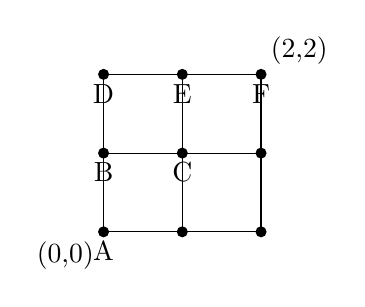
\begin{tikzpicture}
    \coordinate (A) at (0,0);
    \coordinate (B) at (1,0);
    \coordinate (C) at (2,0);
    \coordinate (D) at (0,1); 
    \coordinate (E) at (1,1);
    \coordinate (F) at (2,1);
    \coordinate (G) at (0,2);
    \coordinate (H) at (1,2);
    \coordinate (I) at (2,2);

    

    % Draw the grid
    \draw (A) grid (I);

    % Draw dots at each coordinate
    \foreach \point in {A,B,C,D,E,F,G,H,I} {
        \fill (\point) circle (2pt);
    }

    % Label the corners (0,0) and (1,1) as in the original image
    \node[below left] at (A) {(0,0)};
    \node[above right] at (I) {(2,2)}; % Adjusted to (2,2) for the 3x3 grid

   

    \node[below] at (A) {A}; % (0,0)
    \node[below] at (D) {B}; % (0,1)
    \node[below] at (E) {C}; % (1,1)
    \node[below] at (G) {D}; % (0,2)
    \node[below] at (H) {E}; % (0,2)
    \node[below] at (I) {F}; % (0,2)
\end{tikzpicture}

\section*{Rozwiązanie}

Oznaczmy oczekiwane liczby kroków z poszczególnych wierzchołków odpowiednio:
\[
A = E(0,0), \quad
B = E(1,0), \quad
C = E(1,1), \quad
D = E(2,0), \quad
E = E(2,1), \quad
F = E(2,2)
\]
Ponieważ wierzchołek $(2,2)$ zawiera żołądź, mamy
\[
F = 0.
\]

Dla pozostałych wierzchołków zapisujemy równania dla wartości oczekiwanej:

\[
\begin{cases}
A = 1 + B, \\[6pt]
B = 1 + \frac{1}{3}A + \frac{1}{3}C + \frac{1}{3}D, \\[6pt]
C = 1 + \frac{1}{2}B + \frac{1}{2}E, \\[6pt]
D = 1 + \frac{1}{2}B + \frac{1}{2}C, \\[6pt]
E = 1 + \frac{1}{3}C + \frac{1}{3}D + \frac{1}{3}F.
\end{cases}
\]

Ponieważ $D = C$ , układ upraszcza się do:

\[
\begin{cases}
A = 1 + B, \\[6pt]
B = 1 + \frac{1}{3}A + \frac{2}{3}C, \\[6pt]
C = 1 + \frac{1}{2}B + \frac{1}{2}E, \\[6pt]
E = 1 + \frac{2}{3}C.
\end{cases}
\]

Z ostatniego równania otrzymujemy:
\[
E = 1 + \frac{2}{3}C.
\]

Podstawiając do trzeciego równania:
\[
C = 1 + \frac{1}{2}B + \frac{1}{2}\left(1 + \frac{2}{3}C\right),
\]
czyli
\[
C = \frac{3}{2} + \frac{1}{2}B + \frac{1}{3}C.
\]
Stąd
\[
\frac{2}{3}C = \frac{3}{2} + \frac{1}{2}B \quad \Rightarrow \quad C = \frac{9}{4} + \frac{3}{4}B.
\]

Podstawiając do równania dla $B$:
\[
B = 1 + \frac{1}{3}A + \frac{2}{3}C.
\]
Z $A = 1 + B$ mamy:
\[
B = 1 + \frac{1}{3}(1 + B) + \frac{2}{3}C,
\]
czyli
\[
\frac{2}{3}B = \frac{4}{3} + \frac{2}{3}C \quad \Rightarrow \quad B = 2 + C.
\]

Podstawiamy $C = \frac{9}{4} + \frac{3}{4}B$:
\[
B = 2 + \frac{9}{4} + \frac{3}{4}B,
\]
czyli
\[
\frac{1}{4}B = \frac{17}{4} \quad \Rightarrow \quad B = 17.
\]

Stąd:
\[
C = \frac{9}{4} + \frac{3}{4} \cdot 17 = \frac{9 + 51}{4} = 15, \quad A = 1 + B = 18.
\]

Oczekiwana liczba kroków, jakie wiewiórka wykona zanim znajdzie żołędzia, wynosi \(\mathbf{18}\).

\subsection*{Odpowiedź}
\[
\boxed{\text{18}}
\]

\section{Zadanie 2}
\autor{Hubert Jastrzębski}
Rzucamy kostką, aż nie zanotujemy dwóch szóstek pod rząd. Jaka jest oczekiwana liczba rzutów?

\textit{Wskazówka:} Odpowiedzią nie jest 36.

\subsection*{Rozwiązanie}
Zasada chyba (bo jeszcze nikt go nie spisał) podobna do tej z poprzedniego zadania,
ale nawet trochę prostsza.

Generalnie będziemy chcieli stworzyć układ równań, który pozwoli nam wyliczyć
oczekiwaną liczbę rzutów -- rozpisałem się trochę (+ w vs code ciężko czasem nie kliknąć tego tab), ale samo zadanie nie jest skomplikowane.

Zdefiniujmy sobie trzy stany:
\begin{itemize}
    \item Stan $N$ (neutralny) -- stan w którym w ostatnim rzucie nie wypadła szóstka (albo jest to pierwszy rzut).
    \item Stan $S$ (jedna szóstka) -- stan w którym w ostatnim rzucie wypadła szóstka, ale nie mamy jeszcze dwóch szóstek pod rząd.
    \item Stan $K$ (dwie szóstki, koniec) -- stan w którym mamy już dwie szóstki pod rząd.
\end{itemize}

Niech $X$ będzie zmienną losową, oznaczającą liczbę rzutów potrzebnych do zakończenia gry.

Niech:
\begin{itemize}
    \item $E_N = E(X | \text{ jesteśmy w stanie } N)$ -- oczekiwana liczba rzutów do zakończenia gry, jeśli zaczynamy w stanie $N$,
    \item $E_S = E(X | \text{ jesteśmy w stanie } S)$ -- oczekiwana liczba rzutów do zakończenia gry, jeśli zaczynamy w stanie $S$,
    \item $E_K = E(X | \text{ jesteśmy w stanie } K)$ -- oczekiwana liczba rzutów do zakończenia gry, jeśli zaczynamy w stanie $K$.
\end{itemize}

Oczywiście $E_K = 0$, bo gra się już skończyła.

Rozważmy teraz stan $N$. W tym stanie rzucamy kostką:
\begin{itemize}
    \item Z prawdopodobieństwem $\frac{1}{6}$ wypada szóstka i przechodzimy do stanu $S$.
    \item Z prawdopodobieństwem $\frac{5}{6}$ nie wypada szóstka i pozostajemy w stanie $N$.
\end{itemize}
W każdym przypadku wykonaliśmy jeden rzut, więc możemy zapisać równanie:
\[E_N = \frac{1}{6}(E_S + 1) + \frac{5}{6}(E_N + 1)\]
Podobnie jest ze stanem $S$:
\begin{itemize}
    \item Z prawdopodobieństwem $\frac{1}{6}$ wypada szóstka i przechodzimy do stanu $K$.
    \item Z prawdopodobieństwem $\frac{5}{6}$ nie wypada szóstka i wracamy do stanu $N$.
\end{itemize}
Znowu wykonaliśmy jeden rzut, więc mamy:
\[E_S = \frac{1}{6}(E_K + 1) + \frac{5}{6}(E_N + 1)\]

Teraz pozostaje tylko rozwiązać układ równań (bardzo ciężki):
\begin{align*}
E_N &= \frac{1}{6}(E_S + 1) + \frac{5}{6}(E_N + 1) \\
&= \frac{1}{6}(\frac{1}{6}(E_K + 1) + \frac{5}{6}(E_N + 1) + 1) + \frac{5}{6}(E_N + 1) \\
&= \frac{1}{6}(\frac{1}{6} + \frac{5}{6}E_N + \frac{5}{6} + 1) + \frac{5}{6}(E_N + 1) \\
&= \frac{2}{6} + \frac{5}{36}E_N + \frac{5}{6}E_N + \frac{5}{6} \\
&= \frac{7}{6} + \frac{35}{36}E_N \\
E_N &= \frac{7}{6} \cdot \frac{36}{1} = 42
\end{align*}

Jako iż $N$ to jest stan z którego rozpoczynamy grę, to odpowiedzią jest właśnie $E_N = 42$.

\subsection*{Odpowiedź}
\[
\boxed{\text{42}}
\]

\section{Zadanie 3}
\autor{Dominik Korsa}
Ze standardowej talii 52 kart wyciągamy 13 (ręka brydżowa). Niech \(X\) to
liczba wyciągniętych asów, a \(Y\) to liczba wyciągniętych trefli.

\begin{enumerate}[label=(\roman*)]
  \item\label{set04.task03.1} Czy \(X\) i \(Y\) są niezależne?
  \item\label{set04.task03.2} Czy \(X\) i \(Y\) są nieskorelowane?
\end{enumerate}

\subsection*{Przypomnienie}
Zmienne losowe \(X\) i \(Y\) są \textbf{niezależne}, gdy dla każdego
\(x, y \in \mathbb{R}\):
\[
  P(X=x \land Y=y) = P(X=x) \cdot P(Y=y)
\]

Zmienne losowe \(X\) i \(Y\) są \textbf{nieskorelowane}, gdy:
\[
  E[X \cdot Y] = E[X] \cdot E[Y]
\]

\subsection*{Rozwiązanie podpunktu \ref{set04.task03.1}}
Nie są niezależne, pokażę kontrprzykład.

\begin{itemize}
  \item \(P(X=4)\) to prawdopodobieństwo, że wyciągniemy 4 asy, oczywiście
  \(P(X=4) > 0\).

  \item \(P(Y=13)\) to prawdopodobieństwo, że wyciągniemy tylko trefle, podobnie
  \(P(Y=13) > 0\).

  \item \(P(X=4 \land Y=13)\) to prawdopodobieństwo, że wyciągniemy tylko trefle,
  w tym cztery asy. Takie zdarzenie jest niemożliwe, więc
  \(P(X=4 \land = Y=13) = 0\).
\end{itemize}
Czyli nie jest prawdą, że dla każdego \(x, y \in \mathbb{R}\) zachodzi
\[P(X=x \land Y=y) = P(X=x) \cdot P(Y=y),\]
więc zmienne losowe \(X\) i \(Y\) nie są niezależne.

\subsection*{Rozwiązanie podpunktu \ref{set04.task03.2}}
Niech $X_i$ to indykator zdarzenia, że $i$-ta wylosowana karta to as:
\[
  E[X_i=1] = \frac{4}{52} = \frac{1}{13} \quad\text{(dla \(i \in [13]\))}
\]
Z liniowości wartości oczekiwanej:
\[
  E[X]
  = E[X_1 + \cdots + E_{13}]
  = E[X_1] + \cdots + E[X_{13}]
  = 13 \cdot \frac{1}{13} = 1
\]

Analogicznie niech $Y_i$ to indykator zdarzenia, że $i$-ta karta to trefl:
\[
  E[Y] = \cdots = 13 \cdot \frac{1}{4} = \frac{13}{4}
\]

% Spróbujmy policzyć lub oszacować \(E[XY]\). Skorzystajmy z warunkowej wartości
% oczekiwanej:
% \begin{align*}
%   E[XY]
%   &= \sum_{x=0}^{4} E[XY | X=x] \cdot P(X=x)\\
%   &= \sum_{x=0}^{4} x \cdot E[Y | X=x] \cdot P(X=x)\\
% \end{align*}

% \(P(X=x) = \frac{\binom{4}{x} \cdot \binom{48}{13-x}}{\binom{52}{13}}\)
\(X_iY_i\) to indykator zdarzenia, że \(i\)-ta wylosowana karta to as trefl:
\(E[X_iY_i] = \frac{1}{52}\).

Dla \(i \neq j\) \(X_iY_j\) to indykator zdarzenia, że \(i\)-ta wylosowana karta
jest asem, a \(j\)-ta to trefl. Te zdarzenia są niezależne, więc:
\[
  E[X_iY_j] = P(X_i = 1 \land Y_j = 1)
  = P(X_i = 1) \cdot P(Y_j = 1)
  = \frac{1}{4} \cdot \frac{1}{13} = \frac{1}{52}
\]

Czyli dla każdej pary \((i, j) \in [13] \times [13]\) zachodzi \(E[X_iY_i] = \frac{1}{52}\).

Z liniowości wartości oczekiwanej:
\[
  E[XY]
  = E\left[ \sum_{(i,j) \in [13] \times [13]} X_iY_j \right]
  = \sum_{(i,j) \in [13] \times [13]} E[X_iY_j]
  = 13^2 \cdot \frac{1}{52}
  = \frac{13}{4},
\]
Wiemy też, że:
\[
  E[X] \cdot E[Y] = 1 \cdot \frac{13}{4} = \frac{13}{4},
\]
więc warunek na \textbf{nieskorelowanie} zmiennych losowych \(X\) i \(Y\) zachodzi.

\subsection*{Odpowiedź}
\[
\boxed{\text{\(X\) i \(Y\) \textbf{nie są niezależne}, ale \textbf{są nieskorelowane}}}
\]

\section{Zadanie 4}
Każdy z n graczy rzuca niezależnie od pozostałych kostką.
\begin{enumerate}[label=(\roman*)]
    \item\label{set04.task04.1} Za dowolną parę graczy którzy wyrzucili ten sam wynik grupa dostaje 1 punkt.
    Znaleźć wariancję liczby uzyskanych punktów.
    \item\label{set04.task04.2} Za dowolną parę graczy którzy wyrzucili ten sam wynik grupa dostaje tyle punktów
    ile wyrzucili. Znaleźć wariancję liczby uzyskanych punktów.
\end{enumerate}

\subsection*{Wstęp}
Niech $X_i$ będzie wynikiem rzutu $i$-tego gracza, dla $i = 1, \dots, n$.
Zmienne $X_i$ są niezależne i mają jednakowy rozkład: $P(X_i = k) = \frac{1}{6}$ dla $k \in \{1, 2, 3, 4, 5, 6\}$.

Będziemy korzystać ze wzoru na wariancję sumy zmiennych losowych:
$$\text{Var}\left(\sum_{k} A_k\right) = \sum_{k} \text{Var}(A_k) + \sum_{k \neq l} \text{Cov}(A_k, A_l)$$

\subsection*{Rozwiązanie podpunktu \ref{set04.task04.1}}

Definiujemy zmienną losową $Y$ jako całkowitą liczbę punktów.
Liczba punktów jest sumą punktów przyznanych każdej parze graczy. Jest $\binom{n}{2}$ takich par.

Dla każdej pary graczy $(i, j)$ z $1 \le i < j \le n$, zdefiniujmy indykator $Y_{ij}$:
$$Y_{ij} = \begin{cases} 1 & \text{gdy } X_i = X_j \\ 0 & \text{gdy } X_i \neq X_j \end{cases}$$

Całkowita liczba punktów $Y$ to oczywiście suma tych zmiennych:
$$Y = \sum_{1 \le i < j \le n} Y_{ij}$$

Aby znaleźć $\text{Var}(Y)$, musimy obliczyć $\text{Var}(Y_{ij})$ oraz $\text{Cov}(Y_{ij}, Y_{kl})$ dla $(i,j) \neq (k,l)$.
\subsubsection*{Wariancja}
Wartość oczekiwana: $E[Y_{ij}] = p = \frac{1}{6}$. \\
Wariancja: $\text{Var}(Y_{ij}) = p(1-p) = \frac{1}{6} \left(1 - \frac{1}{6}\right) = \frac{1}{6} \cdot \frac{5}{6} = \frac{5}{36}$.
\subsubsection*{Kowariancja}
Dla par rozłącznych Kowariancja jest równa 0 zastanówmy co dzieje się dla par mających jeden wspólny wskaźnik.
BSO weźmy pary $(i, j)$ i $(i, k)$, wtedy
$$P(Y_{ij} = 1\ \text{i}\ Y_{ik} = 1) = P(\text{wszyscy trzej gracze mają ten sam wynik}) = \frac{1}{36}$$
stąd
$$Cov(Y_{ij}, Y_{ik}) = \frac{1}{36} - (\frac{1}{6})^2 = 0 $$
zatem wszystkie kowariancje pomiedzy dwoma różnymi $Y_{ij}$ są równe $0$
\subsubsection{A zatem}
wariancja sumy jest po prostu sumą wariancji:
$$\text{Var}(Y) = \sum_{1 \le i < j \le n} \text{Var}(Y_{ij})$$
Liczba par $(i, j)$ wynosi $\binom{n}{2} = \frac{n(n-1)}{2}$.
$$\text{Var}(Y) = \binom{n}{2} \cdot \text{Var}(Y_{ij}) = \frac{n(n-1)}{2} \cdot \frac{5}{36} = \frac{5n(n-1)}{72}$$


\subsection*{Rozwiązanie podpunktu \ref{set04.task04.2}}
Definiujemy zmienną losową $Y$ jako całkowitą liczbę punktów.
Dla każdej pary graczy $(i, j)$ z $1 \le i < j \le n$, zdefiniujmy zmienną $Y_{ij}$:
$$Y_{ij} = \begin{cases} X_i & \text{gdy } X_i = X_j \\ 0 & \text{gdy } X_i \neq X_j \end{cases}$$

\subsubsection*{Moment pierwszego i drugiego rzędu}
\[
\E[Y_{ij}] = \sum_{k=1}^{6} k \cdot \frac{1}{36} = \frac{21}{36} = \frac{7}{12},
\]
\[
\E[Y_{ij}^2] = \sum_{k=1}^{6} k^2 \cdot \frac{1}{36} = \frac{91}{36},
\]
\[
Var(Y_{ij}) = \frac{91}{36} - \left(\frac{7}{12}\right)^2 = \frac{35}{16}.
\]

\subsubsection*{Kowariancja dwóch zmiennych}
Jeśli pary są rozłączne, kowariancja = 0.
Jeśli pary mają wspólnego gracza (\(Y_{ij}\) i \(Y_{ik}\)):
\[
\E[Y_{ij}Y_{ik}] = \sum_{k=1}^{6} k^2 \cdot \frac{1}{216} = \frac{91}{216},
\]
\[
Cov(Y_{ij}, Y_{ik}) = \frac{91}{216} - \left(\frac{7}{12}\right)^2 = \frac{35}{432}.
\]

\subsubsection*{Liczba par wskaźników ze wspólnym graczem}
Liczba uporządkowanych par o wspólnym wskaźniku (takich potrzebujemy do sumy) to: \\
\[
2 \cdot 3 \cdot \binom{n}{3} = n(n-1)(n-2).
\]

\subsubsection*{Wariancja całkowita}
Wiemy, że
\[
Y = \sum_{1 \le i < j \le n} Y_{ij}.
\]
Wtedy
\[
\begin{aligned}
\operatorname{Var}(Y)
&= \sum_{\{i,j\}} \operatorname{Var}(Y_{ij})
   + \sum_{\substack{(i < j) \neq (k < l)\\}}
     \operatorname{Cov}(Y_{ij}, Y_{ik})\\[6pt]
&= \binom{n}{2} \cdot \frac{35}{16} + n(n-1)(n-2) \cdot \frac{35}{432}\\[6pt]
&= \frac{35\,n(n-1)}{32} + \frac{35\,n(n-1)(n-2)}{432}\\[6pt]
&= 35 \cdot \frac{n(n-1)(2n+23)}{864}.
\end{aligned}
\]



\subsection*{Odpowiedź}
\[
\boxed{
    \text{(i)}\ \binom{n}{2} \cdot \frac{5}{36} = \frac{5n(n-1)}{72}
    \qquad
    \text{(ii)}\ \frac{35\,n(n-1)(2n+23)}{864}
    }
\]

\section{Zadanie 5 (Filip Manijak)}
W urnie znajduje się $b$ białych kul i $c$ czarnych kul. Wyciągamy kolejno wszystkie kule.  

Wyciągnięta kula daje \emph{zmianę}, jeżeli jej kolor jest różny od koloru kuli wyciągniętej bezpośrednio przed nią.  

Wyciągnięta biała kula daje \emph{dobrą zmianę}, jeżeli bezpośrednio przed nią została wyciągnięta czarna kula.  

\bigskip

Oblicz:  
\begin{enumerate}
    \item oczekiwaną liczbę i wariancję \emph{zmian},  
    \item oczekiwaną liczbę i wariancję \emph{dobrych zmian}.
\end{enumerate}


\subsection*{Rozwiązanie}
\section*{Oczekiwana liczba zmian i wariancja}

Niech w urnie jest $b$ białych kul i $c$ czarnych kul, $N=b+c$. Losujemy wszystkie kule kolejno bez zwracania.  

Dla $i=2,\dots,N$ definiujemy wskaźniki:
\[
X_i = 
\begin{cases}
1, & \text{jeśli } i\text{-ta kula ma inny kolor niż }(i-1)\text{-ta},\\
0, & \text{w przeciwnym razie},
\end{cases}
\]
\\
\[
Y_i = 
\begin{cases}
1, & \text{jeśli } i\text{-ta kula jest biała i poprzednia czarna (dobra zmiana)},\\
0, & \text{w przeciwnym razie}.
\end{cases}
\]

\subsection*{I) Zmiany koloru}

Całkowita liczba zmian koloru:
\[
C = \sum_{i=2}^N X_i.
\]

\subsubsection*{Oczekiwana liczba zmian}

Dla dowolnego $i$:
\[
\Pr(X_i=1) = \Pr(\text{B→W}) + \Pr(\text{W→B}) = \frac{b c}{N(N-1)} + \frac{b c}{N(N-1)} = \frac{2 b c}{N(N-1)}.
\]

Zatem:
\[
\mathbb{E}[C] = (N-1) \cdot \frac{2 b c}{N(N-1)} = \frac{2 b c}{N}.
\]

\subsubsection*{Wariancja — pełna}

Każdy wskaźnik $X_i$ to zmienna Bernoulliego:
\[
\operatorname{Var}(X_i) = p(1-p).
\]

Ogólna formuła wariancji sumy:
\[
\operatorname{Var}(C) = \sum_{i=2}^N \operatorname{Var}(X_i) + 2 \sum_{2 \le i < j \le N} \operatorname{Cov}(X_i, X_j).
\]

\paragraph{1. Kowariancje sąsiadujące (\(|i-j|=1\))}

Niech $X_i$ i $X_{i+1}$ mają wspólną kulę w pozycji $i$. Wtedy:
\[ E[X_iX_{i+1}] = 
\Pr(X_i=1, X_{i+1}=1) = \frac{b c (b-1) + b c (c-1)}{N(N-1)(N-2)} = \frac{bc}{N(N-1)},
\]
więc
\[
\operatorname{Cov}(X_i,X_{i+1}) = \frac{bc}{N(N-1)} - p^2 = \frac{bc}{N(N-1)} - \left(\frac{2bc}{N(N-1)}\right)^2.
\]

Liczba takich par: $(N-2)$.

\paragraph{2. Kowariancje niesąsiadujące (\(|i-j|>1\))}

Niech $X_i$ i $X_j$ nie sąsiadują. Wtedy mamy 4 różne kule w pozycjach $i-1,i,j-1,j$. Zatem:
\[ E[X_iX_{j}] =
\Pr(X_i=1, X_j=1) = \frac{2bc}{N(N-1)} \cdot \frac{2(b-1)(c-1)}{(N-2)(N-3)}.
\]

Liczba takich par: \(\binom{N-1}{2} - (N-2) = \frac{(N-1)(N-2)}{2} - (N-2) = \frac{(N-2)(N-3)}{2}.\)  

Zatem kowariancja dla każdej pary niesąsiadującej:
\[
\operatorname{Cov}(X_i,X_j) = \frac{4bc(b-1)(c-1)}{N(N-1)(N-2)(N-3)} - p^2.
\]

\paragraph{3. Wariancja całkowita}

Sumując:
\[
\operatorname{Var}(C) = (N-1)p(1-p) + 2 (N-2)\Big(\frac{bc}{N(N-1)} - p^2\Big) + 2\cdot \frac{(N-2)(N-3)}{2}\Big(\frac{4bc(b-1)(c-1)}{N(N-1)(N-2)(N-3)} - p^2\Big).
\]

Po uproszczeniu otrzymujemy:
\[
\operatorname{Var}(C) = \frac{2bc(2bc-N)}{N^2(N-1)}.
\]

\subsection*{II) Dobre zmiany}

Dla $i=2,\dots,N$ definiujemy:
\[
Y_i = 
\begin{cases}
1, & \text{jeśli } i\text{-ta kula jest biała i poprzednia czarna (dobra zmiana)},\\
0, & \text{w przeciwnym razie}.
\end{cases}
\]

Całkowita liczba dobrych zmian:
\[
G = \sum_{i=2}^N Y_i.
\]

\subsubsection*{Oczekiwana liczba}

\[
\Pr(Y_i=1) = \frac{bc}{N(N-1)}, \quad \mathbb{E}[G] = (N-1)\frac{bc}{N(N-1)} = \frac{bc}{N}.
\]

\subsubsection*{Wariancja}

Każdy wskaźnik $Y_i$ to zmienna Bernoulliego:
\[
\operatorname{Var}(Y_i) = p(1-p), \quad p = \frac{bc}{N(N-1)}.
\]

Dla sąsiadujących wskaźników $Y_i$ i $Y_{i+1}$:
\[
\operatorname{Cov}(Y_i, Y_{i+1}) = \mathbb{E}[Y_i Y_{i+1}] - \mathbb{E}[Y_i]\mathbb{E}[Y_{i+1}] = 0 - p^2 = -p^2,
\]
ponieważ zdarzenia są rozłączne (kula $i$ nie może jednocześnie być biała i czarna).

Dla niesąsiadujących wskaźników $Y_i, Y_j$ (\(|i-j|>1\)) kowariancja wynosi:
\[
\operatorname{Cov}(Y_i, Y_j) = \Pr(Y_i=1 \text{ i } Y_j=1) - p^2.
\]

Wariancja całkowitej liczby dobrych zmian:
\[
\operatorname{Var}(G) = \sum_{i=2}^N \operatorname{Var}(Y_i) + 2\sum_{2\le i<j\le N} \operatorname{Cov}(Y_i,Y_j).
\]

Po uwzględnieniu wszystkich kowariancji (sąsiadujących i niesąsiadujących) otrzymujemy:
\[
\operatorname{Var}(G) = \frac{b^2 c^2}{N^2 (N-1)}.
\]

\section{Zadanie 6}

Niech \(X\) będzie zmienną losową liczącą liczbę kopii kliki \(K_4\) na czterech wierzchołkach w grafie wylosowanym z modelu \(G_{n,p}\) (to znaczy, mając \(n \geq 4\) wierzchołków dla każdej pary wierzchołków losujemy niezależnie z prawdopodobieństwem \(p \in (0, 1)\), czy są połączone krawędzią, czy nie). Oblicz wartość oczekiwaną i wariancję \(X\).

\subsection*{Rozwiązanie}

Wartość oczekiwana jest prosta do wyliczenia. Wystarczy zdefiniować indykatory \(\{X_I\}_{I \in \binom{V}{4}}\) dla każdego 4-elementowego podzbioru wierzchołków, które są równe 1 wpp. gdy ten zbiór indukuje kopię \(K_4\). Otrzymujemy wartość oczekiwaną:

\[
E[X] = E[\sum_{I \in \binom{V}{4}}X_I] = \sum_{I \in \binom V 4}E[X_I] = \sum_{I \in \binom V 4}p^6 = \binom{n}{4}p^6
\]

Z wariancją jest nieco więcej zabawy, ale na szczęście możemy zauważyć, że indykatory zbiorów o 0 lub 1 wspólnych wierzchołkach byłyby rozłączne krawędziowo, więc byłyby niezależne (a więc \(Cov(X_I, X_J) = 0\)). Możemy więc wyliczyć wariancję pierwsze poznając wartości kowariancji dla przecinających się krawędziowo zbiorów.

\subsubsection*{2 wspólne wierzchołki}

Niech \(X, Y \in \binom{V}{4}, |X \cap Y| = 2\).

\begin{align*}
    Cov(X_I, X_J) &= E[X_IX_J] - E[X_I]E[X_J] =\\
    &= p^{11} - (p^{6})^2 = (1-p)p^{11}
\end{align*}

\subsubsection*{3 wspólne wierzchołki}

Niech \(X, Y \in \binom{V}{4}, |X \cap Y| = 3\)

\begin{align*}
    Cov(X_I, X_J) &= E[X_IX_J] - E[X_I]E[X_J] =\\
    &= p^9 - (p^6)^2 = (1-p^3)p^9
\end{align*}

\subsubsection*{Wariancje}

Pozostaje jeszcze tylko wyliczyć wariancję pojedynczego indykatora:

\[
Var(X_I) = E[X_I^2] - E[X_I]^2 = p^6 - p^{12} = (1-p^6)p^6
\]

I ostateczny wynik:

\begin{align*}
Var(X) &= Var(\sum_{I \in \binom V 4}X_I) = \sum_{I \in \binom V 4}Var(X_I) + \sum_{I, J \in \binom V 4, I \neq J}Cov(X_I, X_J)\\
&= \sum_{I \in \binom V 4}Var(X_I) + \sum_{I, J \in \binom V 4, I \cap J = 2}Cov(X_I, X_J) + \sum_{I, J \in \binom V 4, I \cap J = 3}Cov(X_I, X_J)\\
&= \sum_{I \in \binom V 4}Var(X_I) + \sum_{I, J \in \binom V 4, I \cap J = 2}Cov(X_I, X_J) + \sum_{I, J \in \binom V 4, I \cap J = 3}Cov(X_I, X_J)\\
&= \binom{n}{4}(1-p^6)p^6 + \binom{n}{6}\binom{6}{2}\binom{4}{2}(1-p)p^{11} + \binom{n}{5}\binom{5}{3}\binom{2}{1}(1-p^3)p^9\\
&= \binom{n}{4}(1-p^6)p^6 + 90\binom{n}{6}(1-p)p^{11} + 20\binom{n}{5}(1-p^3)p^9\\
\end{align*}

\subsection*{Odpowiedź}
\[
\boxed{E[X] = \binom{n}{4}p^6, Var[X] \text{ powyżej}}
\]

\section{Zadanie 7}
Powiedzmy, że w urnie znajduje się $N$ kul z czego $K$ jest zielonych a reszta czerwone. Losujemy $n$ kul bez zwracania. 
Niech $X$ będzie liczbą zielonych kul które wylosowaliśmy. Jaki rozkład ma $X$? Innymi słowy, ile wynosi $P(X = k)$?

\subsection*{Rozwiązanie}
$k$ kul zielonych spośród wszystkich kul zielonych można wybrać na $\binom{K}{k}$ sposobów, analogicznie $n-k$ kul czerwonych na $\binom{N-K}{n-k}$ sposobów. Wszystkich sposobów na wybranie $n$ kul ze zbioru $N$ kul jest $\binom{N}{n}$. Wynik wynosi więc:

\[
\frac{\binom{K}{k} \cdot \binom{N-K}{n-k}}{\binom{N}{n}}
\]

\subsection*{Odpowiedź}
\[
\boxed{\frac{\binom{K}{k} \cdot \binom{N-K}{n-k}}{\binom{N}{n}} \text{, jest to rozkład hipergeometryczny}}
\]

\section{Zadanie 8}
Jaka jest wartość oczekiwana i wariancja zmiennej losowej $X$ z poprzedniego zadania.

\subsection*{Rozwiązanie}
Robimy zdarzenie $X_i$, czyli, że i-ta kula jest zielona. Z liniowości wartości oczekiwanej, wiemy, że $E(X) = \sum_{i = 0}^{n} E(X_i)$.

$E(X_i) = P(X_i) = \frac{K}{N}$, więc $E(X) = n * \frac{K}{N}$.

Teraz obliczmy $E(X^2)$, możemy to rozpisać, jako $E(X (X-1) + X) = E(X*(X-1)) + E(X)$.

Teraz powiedzmy, sobie czym jest $E(X*(X-1))$. Bedzie to liczba uporządkowanych par, takich, że obie kule są zielone. 

Wiemy, że takich par będzie $2 * \binom{K}{2}$, a prawdopodobieństwo, że konkretna para się znajdzie to $\frac{\binom{N-2}{n-2}}{\binom{N}{n}}$. Także korzystając z liniowości, wychodzi nam, że: 
\[
E(X*(X-1)) = 2 * \binom{K}{2} * \frac{\binom{N-2}{n-2}}{\binom{N}{n}} = \frac{K*(K-1) * (n) * (n-1)}{(N)*(N-1)}
\]
\[
    Var(X) = E(X^2)-E(X)^2 = \frac{K*(K-1) * n * (n-1)}{N*(N-1)} + n * \frac{K}{N} - (n*\frac{K}{N})^2
\]
\[
    Var(X) = \frac{n*K}{N} * (\frac{(K-1) * (n-1)}{(N-1)} + 1 - (n*\frac{K}{N}))
\]
\[
    Var(X) = \frac{n*K}{N} * (\frac{(K-1) * (n-1)}{(N-1)} + \frac{N-1}{N-1} - (n*\frac{K}{N}))
\]
\[
    Var(X) = \frac{n*K}{N} * (\frac{(K-1) * (n-1) + (N-1)}{(N-1)} - (n*\frac{K}{N}))
\]
\[
    Var(X) = \frac{n*K}{N} * (\frac{K * (n-1) - n + N}{(N-1)} - (n*\frac{K}{N}))
\]
\[
    Var(X) = \frac{n*K}{N} * \frac{N*K*(n-1) - n*N + N^2 - n * K * (N-1)}{N * (N-1)}
\]
\[
    Var(X) = \frac{n*K}{N} * \frac{K * (N * (n-1) - n * (N-1)) - n*N + N^2}{N * (N-1)}
\]
\[
    Var(X) = \frac{n*K}{N} * \frac{K * ( - N + n ) - n*N + N^2}{N * (N-1)}
\]
\[
    Var(X) = \frac{n*K*(N-n)}{N} * \frac{-K + N}{N * (N-1)}
\]
\[
    Var(X) = \frac{n*K*(N-n)}{N*(N-1)} * (1 - \frac{K}{N})
\]
\subsection*{Odpowiedź}
\[
\boxed{\text{$E(X) = n * \frac{K}{N}$, $Var(X) = \frac{n*K*(N-n)}{N*(N-1)} * (1 - \frac{K}{N})$}}
\]

\section{Zadanie 9}
Pokaż, że nierówność Markowa jest optymalna. To znaczy, dla danego \(a > 1\) znajdź zmienną losową \(X\), że:

\[P(X\geqslant aE(X)) = \frac{1}{a}\]

\subsection*{Rozwiązanie}
Niech dla naszej zmiennej losowej \(P(X = 0) = \frac{a-1}{a}\) oraz \(P(X = a) = \frac{1}{a}\).

Wtedy \(E(X) = P(X = 0)\cdot 0 + P(X = a)\cdot a = \frac{a-1}{a}\cdot 0 + \frac{1}{a}\cdot a = 1\),

stąd mamy, że \(P(X\geqslant aE(X)) = P(X\geqslant a) = P(X = a) = \frac{1}{a}\).

\subsection*{Odpowiedź}
\[
	\boxed{\text{\(P(X = 0) = \frac{a-1}{a}\) oraz \(P(X = a) = \frac{1}{a}\)}}
\]

\section{Zadanie 10 (Kacper Orszulak)}
Algorytm bąbelkowy sortowania przegląda podaną na wejściu permutację i odwraca sąsiadujące elementy bądace w inwersji. Przejścia wzdłuż permutacji są powtarzane tak długo, aż permutacja jest posortowana. Załóż, że podajemy temu algorytmowi losowo wybraną permutację zbioru $[n]$. Jaka jest oczekiwana liczba inwersji, którą odwróci algorytm podczas swojego działania. Jaka jest wariancja? Za pomocą nierówności Czebyszewa pokaż, że algorytm sortowania bąbelkowego wykonuje prawie zawsze liczbę kroków rzędu $\Omega(n^2)$.

\subsection*{Rozwiązanie}

\subsubsection*{Wstęp}
Zamiana miejscami dwóch sąsiednich elementów będących w inwersji zmniejsza ogólną liczbę inwersji dokładnie o jeden. Z tego powodu liczba zamian w algorytmie jest równa liczbie inwersji w wejściowej permutacji. W zadaniu będziemy zatem analizować własności zmiennej losowej $X$ będącą liczbą inwersji wylosowanej permutacji.

Niech $X_{ij}$ to indykator tego, czy dla $i < j$ zachodzi $\sigma(i) > \sigma(j)$. Oczywiście $X = \sum_{1 \le i < j \le n} X_{ij}$.

Zachodzi $\mathcal{P}(X_{ij} = 1) = \frac{n(n-1)/2}{n(n-1)} = \frac{1}{2}$.

Ponadto dla indykatorów zachodzi $\mathbb{E}(X_{ij}^2) = \mathbb{E}(X_{ij}) = \mathcal{P}(X_{ij} = 1)$. Zatem $Var(X_{ij}) = \frac{1}{4}$.

\subsubsection*{Wartość oczekiwana liczby zamian}
\[
    \mathbb{E}(X) = \sum_{1 \le i < j \le n} \mathbb{E}(X_{ij}) = \sum_{1 \le i < j \le n} \mathcal{P}(X_{ij} = 1) = \binom{n}{2} \cdot \frac{1}{2} = \frac{n(n-1)}{4}
\]

\subsubsection*{Wariancja liczby zamian}

\textbf{Lemat.} \textit{Wariancja sumy $n$ zmiennych losowych.}
\[
    Var\left(\sum_{i \in [n]} X_{i}\right) = \sum_{i \in [n]} Var(X_i) + 2 \sum_{\{i, j\} \in \binom{[n]}{2}} Cov(X_i, X_j)
\]
\textbf{Dowód.} \textit{Pozostawiam jako ćwiczenie dla czytelnika ;).}

Wracając do zadania:

\[
    Var(X) = Var\left(\sum_{\{i,j\} \in \binom{[n]}{2}} X_{ij}\right) = \sum_{\{i,j\} \in \binom{[n]}{2}} Var(X_{ij}) + 2 \sum_{\{\{i,j\}, \{k,l\}\} \in \binom{\binom{[n]}{2}}{2}} Cov(X_{ij}, X_{kl})
\]

Zastanówmy się teraz jak obliczyć sumę kowariancji.

Jeżeli rozważymy składnik taki, że $i, j, k, l$ są parami różne, to dostaniemy zmienne $X_{ij}, X_{kl}$, które na pewno są niezależne, ponieważ nierówność $\sigma(i) \substack{<\\ >} \sigma(j)$ nie wpływa na nierówność $\sigma(k) \substack{<\\ >} \sigma(l)$. Oznacza to, że $Cov(X_{ij}, X_{kl}) = 0$.

Nie może się zdarzyć, że $i = j = k = l$, ponieważ $\{i, i\} = \{i\} \not \in \binom{[n]}{2}$.

Analogicznie nie może zajść, że $i = j \; \lor \; k = l$. Nie może też zajść $i = k \; \land \; j = l$.

Pozostaje nam zatem rozważyć tylko przypadek, że $|\{i, j, k, l\}| = 3$.

Niech zatem $\{p, q, r\} \in \binom{[n]}{3}$ takie że $p < q < r$. BSO załóżmy, że $i < j \; \land \; k < l$ oraz $(i, j) \overset{\text{leksykograficznie}}{<} (k, l)$.

Oto składniki, których jeszcze nie rozważyliśmy:
\[
    Cov(X_{pq}, X_{pr}) + Cov(X_{pr}, X_{qr}) + Cov(X_{pq}, X_{qr})
\]

Wiemy, że $Cov(X, Y) = \mathbb{E}(XY) - \mathbb{E}(X)\mathbb{E}(Y)$ \footnote{Na wykładzie i w P\&C chyba nie ma tego wzoru, ale jest powszechnie znany.}. Jedyne czego jeszcze nie wiemy zatem, to wartości oczekiwane iloczynów zmiennych losowych. Każdy iloczyn indykatorów, to też indykator, a więc wystarczy policzyć tylko prawdopodobieństwa postaci $\mathcal{P}(X_{ij}X_{kl} = 1) = \mathcal{P}(X_{ij} = 1 \land X_{kl} = 1)$.

$\mathcal{P}(X_{pq} = 1 \land X_{pr} = 1) = P\left(\left\{\substack{\sigma_p > \sigma_q\\ \sigma_p > \sigma_r} \right. \right) = \frac{1}{3}$, ponieważ jest $\frac{2!}{3!}$ permutacji, w których $\sigma_p$ jest największe. Zatem $Cov(X_{pq}, X_{qr}) = \frac{1}{3} - \frac{1}{4} = \frac{1}{12}$.

$\mathcal{P}(X_{pr} = 1 \land X_{qr} = 1) = P\left(\left\{\substack{\sigma_p > \sigma_r\\ \sigma_q > \sigma_r} \right. \right) = \frac{1}{3}$, ponieważ jest $\frac{2!}{3!}$ permutacji, w których $\sigma_r$ jest najmniejsze. Zatem $Cov(X_{pr}, X_{qr}) = \frac{1}{3} - \frac{1}{4} = \frac{1}{12}$.

$\mathcal{P}(X_{pq} = 1 \land X_{qr} = 1) = P\left(\sigma_p > \sigma_q > \sigma_r \right) = \frac{1}{6} = \frac{1}{3!}$, ponieważ nie mamy żadnej swobody w permutacji trzyelementowej. Zatem $Cov(X_{pq}, X_{qr}) = \frac{1}{6} - \frac{1}{4} = -\frac{1}{12}$.

Dokończymy obliczenia:
\[
    Var(X) = \binom{n}{2} \cdot \frac{1}{4} + 2 \cdot \binom{n}{3} \cdot \left(\frac{1}{12} + \frac{1}{12} - \frac{1}{12}\right) = \frac{n(n-1)(2n+5)}{72}
\]

\subsubsection*{Prawdopodobieństwo odchyłu}
\textbf{Twierdzenie.} \textit{Nierówność Czebyszewa} Dla dowolnego $a > 0$
\[
    \mathcal{P}(|X - \mathbb{E}[X]| \ge a) \le \frac{Var[X]}{a^2}
\]

Niech $\mu := \mathbb{E}[X]$, $\alpha \in (0; 1)$ oraz $a := (1 - \alpha)\mu$.

Policzmy prawdopodobieństwo, że liczba inwersji jest co najwyżej $O(n^2)$.
\begin{align*}
    \mathcal{P}(X = O(n^2)) &= \mathcal{P}(X \le \alpha \mu) = \mathcal{P}(\mu - X \ge (1 - \alpha) \mu) = \\
    &= \mathcal{P}(\mu - X \ge a) \le \mathcal{P}(\left|X - \mu\right| \ge a) \\
    &\le \frac{Var[X]}{(1-\alpha)^2\mu^2} = \frac{8}{9} \frac{2n+5}{n(n-1)} \frac{1}{(1-\alpha)^2} \\
    &\xrightarrow[n\to\infty]{} 0
\end{align*}

Zatem
\[
    \mathcal{P}(X = \Omega(n^2)) = 1 - \mathcal{P}(X = O(n^2)) \xrightarrow[n\to\infty]{} 1 - 0 = 1
\]
Dostajemy więc szukaną tożsamość. $\square$

\subsection*{Odpowiedź}
\[
\boxed{\mathbb{E}(X) = \frac{n(n-1)}{4}, \; Var[X] = \frac{n(n-1)(2n+5)}{72}}
\]

\section{Zadanie 11}
Losujemy słowo binarne długości \(n\). Rozważmy wszystkie \(\binom{n}2\)
par indeksów. Dla każdej takiej pary zmienna \(X_{ij}\) jest wartością
funkcji xor na \(i\)-tym oraz \(j\)-tym bicie. Niech X = 
\(\sum_{1\leqslant i < j \leqslant n} X_{ij}\).

\begin{enumerate}[label=(\roman*)]
  \item wykaż, że zmienne nie są niezależne jako rodzina zmiennych
  \item wykaż, że \(\mathbb{E}(X_{ab}X_{cd}) = 
    \mathbb{E}(X_{ab}) \mathbb{E}(X_{cd})\) dla 
    \(\{a, b\} \neq \{c, d\}\)
  \item wyznacz Var(\(X\)) korzystając z poprzedniego podpunktu
  \item przy pomocy nierówności Czebyszewa ogranicz
  \(P(|X-E(X)|\geqslant n)\)
\end{enumerate}

\subsection*{Rozwiązanie}
\subsubsection*{(i)}
Zakładamy \(n \geqslant 3\) (dla mniejszego \(n\) jest \(\leqslant 1\) 
zmiennych losowych, więc na pewno są niezależne)

Oczywiście \(P(X_{ij} = 0) = P(X_{ij} = 1) = \frac{1}{2}\quad
\forall_{1\leqslant i < j \leqslant n}\)

Weźmy trzy bity \(A_1, A_2\) i \(A_3\). 

Zdarzenie \((X_{12} = 1 \land X_{13} = 1 \land X_{23} = 1)\)
wymaga \(A_1 \neq A_2, A_1 \neq A_3\) i \( A_2 \neq A_3\),
co nie jest możliwe jednocześnie.

Otrzymujemy \(P(X_{12} = 1 \land X_{13} = 1 \land X_{23} = 1) = 0
\neq \frac{1}{8} = P(X_{12} = 1) P(X_{13} = 1) P(X_{23} = 1)\) 

\subsubsection*{(ii)}
Jeśli \(\{a, b\} \cap \{c, d\} = \emptyset\) to trywialne - \(X_{ab}\) i \(X_{cd}\)
są niezależne.

Wpp. bez straty ogólności niech \(a = c\), \(b \neq d\).
Wartości bitów \(A_a, A_b, A_d\) są niezależne i z równym prawdopodobieństwem
równe \(0\) lub \(1\).

Oczywiście
\(E(X_{ab}) = P(X_{ab} = 1) = P(A_a \neq A_b) = \frac{1}{2}
= E(X_{ad}) = E(X_{bd})\)

\(E(X_{ab}X_{ad}) = P(X_{ab} = 1 \land X_{ad} = 1) = P(A_a \neq A_b \land 
A_a \neq A_d)\)\\
\(= P(A_b = A_d = 1 | A_a = 0)P(A_a = 0) + P(A_b = A_d = 0 | A_a = 1)P(A_a = 1)
\)

Skoro \(A_a, A_b, A_d\) są niezależne, to można podstawić wszędzie
\(\frac{1}{2}\)

\(E(X_{ab}X_{ad}) = \left(\frac{1}{2}\right)^3
+ \left(\frac{1}{2}\right)^3 = \frac{1}{4}
= E(X_{ab})E(X_{ad})
\)

\subsubsection*{(iii)}
Skoro każda para zmiennych jest niezależna, to wariancja sumy jest
sumą wariancji.
\[\text{Var}(\sum_{1\leqslant i < j \leqslant n} X_{ij})
= \sum_{1\leqslant i < j \leqslant n} \text{Var}(X_{ij})
= \binom{n}{2} \cdot \frac{1}{4}
\]

\subsubsection*{(iv)}
\[
    P(|X-E(X)|\geqslant n)\) \leqslant \frac{\text{Var}(X)}{n^2}
    = \frac{\frac{1}{8}n(n-1)}{n^2} = \frac{n-1}{8n} < \frac{1}{8}
\]

\subsection*{Odpowiedź (iv)}
\[
\boxed{\frac{n-1}{8n}}
\]

\section{Zadanie 12}
Niech \(X_1, X_2, \ldots, X_n\) będą niezależnymi zmiennymi losowymi z tego samego rozkładu o skończonej wartości oczekiwanej \(\mu\)
oraz skonczonym odchyleniu standardowym \(\sigma\). Na bazie nierówności Czebyszewa pokaż, że dla kazdego \(\epsilon > 0\)

\[\lim_{n \to \infty} P\left(\left|\frac{X_1 + X_2 + \ldots + X_n}{n} - \mu\right| > \epsilon\right) = 0\]

\subsection*{Rozwiązanie}
Zauważmy, że \(\frac{X_1 + X_2 + \ldots + X_n}{n}\) jest średnią arytmetyczną zmiennych losowych \(X_i\). Zastosujmy nierówność Czebyszewa:

\[P\left(\left|\frac{X_1 + X_2 + \ldots + X_n}{n} - \mu\right| > \epsilon\right) \leq \frac{\variance{\frac{X_1 + X_2 + \ldots + X_n}{n}}}{\epsilon^2}\]

Obliczmy wariancję średniej:

\[\variance{\frac{X_1 + X_2 + \ldots + X_n}{n}} = \frac{1}{n^2} \sum_{i=1}^n \variance{X_i} = \frac{\sigma^2}{n}\]

Podstawiając to do nierówności Czebyszewa, otrzymujemy:

\[P\left(\left|\frac{X_1 + X_2 + \ldots + X_n}{n} - \mu\right| > \epsilon\right) \leq \frac{\sigma^2/n}{\epsilon^2} = \frac{\sigma^2}{n\epsilon^2}\]

Zauważmy, że gdy \(n \to \infty\), to \(\frac{\sigma^2}{n\epsilon^2} \to 0\). Zatem:

\[\lim_{n \to \infty} P\left(\left|\frac{X_1 + X_2 + \ldots + X_n}{n} - \mu\right| > \epsilon\right) = 0\]

\subsection*{Odpowiedź}
\[
	\boxed{\text{Tak to prawda}}
\]

\section{Zadanie 13 (Oskar Prusik)}
Wyznacz postać jawną funkcji tworzącej momenty dla rozkładu jednostajnego na zbiorze [n].

\subsection*{Rozwiązanie}
Zmienna $X$ ma rozkład jednostajny dyskretny na zbiorze $\{1, 2, \dots, n\}$:
\[
P(X = k) = \frac{1}{n} \quad \text{dla } k = 1, 2, \dots, n
\]

Definicja funkcji tworzącej momentów (MGF)
\[
M_X(t) = E(e^{tX}) = \sum_{k=1}^n e^{tk} \cdot P(X = k)
\]


\[
M_X(t) = \sum_{k=1}^n e^{tk} \cdot \frac{1}{n} = \frac{1}{n} \sum_{k=1}^n (e^t)^k
\]


\[
\sum_{k=1}^n (e^t)^k = e^t \cdot \frac{1 - (e^t)^n}{1 - e^t} = e^t \cdot \frac{1 - e^{nt}}{1 - e^t}
\]

\[
M_X(t) = \frac{1}{n} \cdot e^t \cdot \frac{1 - e^{nt}}{1 - e^t}
\]

Dla $t = 0$ otrzymujemy nieoznaczoność, ale z definicji:
\[
M_X(0) = E(e^{0 \cdot X}) = E(1) = 1
\]



\subsection*{Odpowiedź}
\[
\boxed{M_X(t) = \frac{e^t (1 - e^{nt})}{n(1 - e^t)}
		
		dla $t \neq 0$, oraz $M_X(0) = 1$.}}
\]

\section{Zadanie 14}
Wyznacz postać jawną funkcji tworzącej momenty dla rozkładu dwumianowego z parametrami \(n\) i \(p\) na dwa sposoby:

\begin{enumerate}
	\item Oblicz \(\ev{e^{tX}}\) z definicji wartości oczekiwanej.
	\item Skorzystaj z niezależności zmiennych Bernoulliego.
\end{enumerate}

Jak na podstawie funkcji tworzącej dla rozkładu wyznaczyć wartość oczekiwaną i wariancję tego rozkładu?

\subsection*{Rozwiązanie}
\begin{enumerate}
	\item \(\ev{e^{tX}} = \sum_{j = 0}^{n} \binom{n}{j}p^j(1-p)^{n-j}e^{tj} = \sum_{j = 0}^{n} \binom{n}{j}(pe^t)^j(1-p)^{n-j} = (pe^t + (1 - p) )^n = (1 - p + pe^t)^n\)
	\item Jako, iż \(X\) jest zmienną losową z rozkładem dwumianowym to  \(X = X_1 + ... + X_n\), gdzie \(X_i\) jest indykatorem sukcesu w \(i\)-tej próbie, a zmienne \(X_i\) są niezależne. Wtedy \(\ev{e^{tX}} = \ev{e^{t(X_1 + ... + X_n)}} = \ev{\prod_{i = 1}^{n} e^{tX_i}} = \prod_{i = 1}^{n} \ev{e^{tX_i}} = \prod_{i = 1}^{n} (pe^{t} + (1-p)) = (1 - p + pe^{t})^n \)
\end{enumerate}

\(M_X^{(1)}(t) = npe^t(1 - p + pe^t)^{n-1}\)

\(\ev{X} = M_X^{(1)}(0) = np\)

\(M_X^{(2)}(t) = npe^t(1 - p + npe^t)(1 - p + pe^t)^{n-2}\)

Var\((X) = \ev{X^2} - \ev{X}^2 = M_X^{(2)}(0) - M_X^{(1)}(0)^2 = np(1- p + np) - (np)^2 = np(1-p)\)



\chapter{Zestaw 5 -- Nierówność Czernowa}
\chaptermark{Zestaw 5}
\graphicspath{{chapters/zestaw-05/}}
\section{Zadanie 1}
Przeczytaj Sekcję 4.3 \textit{Better Bounds for Some Special Cases} (Twierdzenie
4.7, Wnioski 4.8-4.10 oraz ich dowody).

\section{Zadanie 2}
Tasujemy talię rozróżnialnych kart. W talii mamy $B$ białych kart i $C$ czarnych kart. Niech $r$ będzie ustaloną liczbą, taką że $1 \leq r \leq C$. Wykładamy karty dopóki nie odkryjemy $r$ czarnych kart. Niech $X$ będzie liczbą odkrytych białych kart. Jaki rozkład ma $X$?

\subsection*{Rozwiązanie}
\[
P(X=k) = \frac{\binom{k+r-1}{k}\cdot \binom{B+C-k-r}{B-k}}{\binom{B+C}{B}}
\]\\
Wyjaśnienie: \\
Rozważamy na ile sposobów mogą być ułożone wszystkie karty (nie przestajemy odkrywać kart po odkryciu $r$-tej czarnej)\\
Mamy $\binom{B+C}{B}$ możliwości na wybranie miejsc dla białych kart.\\
Teraz policzymy ułożenia kart, gdzie przez $r$-tą czarną jest $k$ białych. Na $\binom{k+r-1}{k}$ sposobów wybieramy miejsca na białe karty, które mają się znaleźć przed $r$-tą czarną, a na $\binom{B+C-k-r}{B-k}$ sposobów wybieramy miejsca na pozostałe białe karty.

\subsection*{Odpowiedź}
\[
\boxed{\text{$P(X=k) = \frac{\binom{k+r-1}{k} \cdot \binom{B+C-k-r}{B-k}}{\binom{B+C}{B}}$}}
\]

\section{Zadanie 3}
\autor{Aleksander Wieczorek}
Jaka jest wartość oczekiwana i wariancja zmiennej X z poprzedniego zadania?
\subsection*{Rozwiązanie}
Załóżmy że w talii mamy tylko C czarnych nierozróżnialnych kart. Jeśli je ponumerujemy możemy wskazać r-tą z nich. Teraz zdefiniujmy indykator:
\[X_i=\begin{cases}
		1\text{ - jeśli i-ta karta będzie odkryta} \\
		0 \text{ - w p.p.}
	\end{cases}\]
fakt, że i-ta karta będzie odkryta jest równoważny z tym, że znajduje się przed r-tą czarną kartą w talii.\\
Możemy teraz rozważyć dla każdej i-tej karty gdzie może się znaleźć względem czarnych kart:
\vspace{5mm}
\begin{figure}[ht!]
	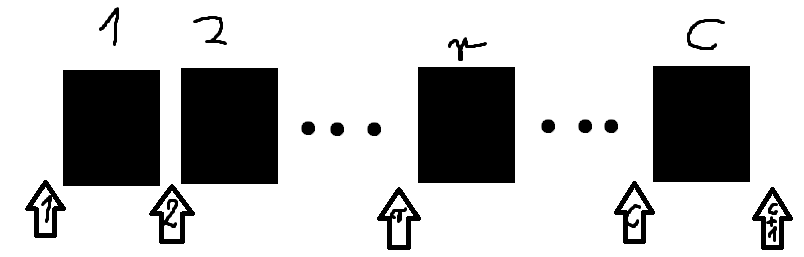
\includegraphics[width=\textwidth]{./tasks/03.png}
	\caption{Gdzie może trafić biała karta}
	\label{fig:placeholder}
\end{figure}
Z własności indykatorów i rysunku dostajemy:
\[E(X_i)=P(X_i=1)=\frac{r}{C+1}\]
A z liniowości mamy:
\[E(X)=E(\sum_{i=1}^B X_i)=\sum_{i=1}^BE(X_i) = B\frac{r}{C+1}\]
Teraz możemy policzyć wariancję.
\[Var(X)=E(X^2)-E(X)^2\]
\[E(X^2)=\sum_{i=1}^B E(X_i^2) + \sum_{i\ne j} E(X_iX_j)\]
Z własności indykatorów mamy \(E(X_i^2)=E(X_i)\), dla 2. części sumy:
\[E(X_iX_j)=P(X_i=1\cap X_j=1) =\frac{r}{C+1}\frac{r+1}{C+2}  \]
1. przekształcenie wynika z własności indykatorów, w 2. po wstawieniu poprawnie 1. karty pojawia się dodatkowy slot, który jest dobry.
Wracając:
\[E(X^2)=B\frac{r}{C+1} + B(B-1)\frac{r}{C+1}\frac{r+1}{C+2} \]
podstawiając do wariancji:
\[Var(X)=B\frac{r}{C+1} + B(B-1)\frac{r}{C+1}\frac{r+1}{C+2}  -  \left(B\frac{r}{C+1}\right)^2\]
\[=\frac{Br}{C+1}\left( 1 +\frac{(B-1)(r+1)}{C+2}-\frac{Br}{C+1}   \right)\]
\subsection*{Odpowiedź}
\[E(X)= \frac{Br}{C+1}\]
\[Var(X)=\frac{Br}{C+1}\left( 1 +\frac{(B-1)(r+1)}{C+2}-\frac{Br}{C+1}   \right)\]

\section{Zadanie 4}
Zmienna losowa \(X\) jest skoncentrowana na zbiorze \(D\), jeśli \(P(X \in D) = 1\). Mówimy, że zmienna losowa \(X\) skoncentrowana na \(\mathbb{N}\) jest bez pamięci jeśli dla każdego \(m, n \in N\) mamy

\[
	P(X > n) > 0 \text{ oraz } P(X = m + n |  X > n).
\]
Wykaż, że jeśli X jest bez pamięci to \(X\) ma rozkład geometycznych.

\subsection*{Rozwiązanie}
Naszym celem, jest pokazanie, że \(X\) ma rozkład geomentryczny. Dowiedziemy to, przez sprawdzenie ilorazu \(\frac{P(N+1)}{P(N)}\).

\[
	\frac{P(x=N+1)}{x=P(N)} = \frac{P(x=N+1)}{P(x=N+1 | x > 1)} =  \frac{P(x=N+1) \cdot P(x > 1)}{P(x = N+1 \wedge x > 1)} =
\]
\[
	\frac{P(x=N+1) \cdot P(x > 1)}{P(x=N+1)} = P(x > 1) = 1 - P(x = 1)
\]
Z tego wyszło, że kolejny element jest poprzednim przemonożonym przez \(1 - P(x = 1)\). Także z tego można wywniskować, że \(P(X = n) = (1-P(X=1))^{n-1} \cdot P(X = 1)\). Co jest definicją rozkładu geometrycznego.

\section{Zadanie 5}
Niech $X_{1},\dots,X_{m}$ będą ciągiem zmiennych losowych indykatorowych o tym samym rozkładzie i niech $\mu = E(X_{i})$.
Jeśli $m \geqslant (3ln(2/\delta)/(\varepsilon^{2}\mu)$.
$$P\left(\left|\frac{1}{m}\sum_{i=1}^{m}X_{i}-\mu\right|\geqslant\varepsilon\mu\right) \leqslant \delta$$

\subsection*{Rozwiązanie}
$$P\left(\left|\frac{1}{m}\sum_{i=1}^{m}X_{i}-\mu\right|\geqslant\varepsilon\mu\right) = P\left(\left(\frac{1}{m}\sum_{i=1}^{m}X_{i}-\mu\geqslant\varepsilon\mu\right)\cup\left(-\frac{1}{m}\sum_{i=1}^{m}X_{i}+\mu\geqslant\varepsilon\mu\right)\right) = $$
$$= P\left(\frac{1}{m}\sum_{i=1}^{m}X_{i}-\mu\geqslant\varepsilon\mu\right) + P\left(\frac{1}{m}\sum_{i=1}^{m}X_{i}-\mu\leqslant-\varepsilon\mu\right)$$

Z twierdzenia 4.4 i 4.5 mamy:
dla $0 < \varepsilon \leqslant 1$
$$ P\left(\sum_{i=1}^{m}X_{i}-m\mu\geqslant m\varepsilon\mu\right) \leqslant e^{-\mu\varepsilon^2m/3}$$
dla $0 < \varepsilon < 1$
$$ P\left(\sum_{i=1}^{m}X_{i}-m\mu\leqslant-m\varepsilon\mu\right) \leqslant e^{-\mu\varepsilon^2m/3}$$
z tego że $X_{i}$ indykator i oszacowania $m$, mamy że $0 < \mu \leqslant 1$, dla tego druga nierówność może być
rozszerzona na $0 < \varepsilon$.

Wtedy dla $0 < \varepsilon \leqslant 1$:
$$P\left(\left|\frac{1}{m}\sum_{i=1}^{m}X_{i}-\mu\right|\geqslant\varepsilon\mu\right) \leqslant 2e^{-\mu\varepsilon^2m/3} \leqslant 2e^{-\mu\varepsilon^2 3ln(2/\delta)/3\varepsilon^{2}\mu} = 2e^{ln(2/\delta)} = \delta$$
\section{Zadanie 6}
\autor{Kacper Orszulak}
Alicja i Bob rozgrywają pomiędzy sobą $n$ pojedynków. Alicja jest lepsza i każdy pojedynek wygrywa niezależnie od pozostałych z prawdopodobieństwem 0.6. Zwycięzcą jest osoba, która wygra więcej pojedynków. Za pomocą nierówności Czernowa ogranicz prawdopodobieństwo tego, że zwycięzcą jest Bob.

\subsection*{Rozwiązanie}
Niech $X_i$ to indykator tego, że Alicja wygrała z Bobem w $i$-tym pojedynku. Dostajemy $\mathcal{P}(X_i = 1) = 0.6 = p$. Niech $X = \sum_{i \in [n]} X_i$ oznacza ilość wygranych przez Alicję pojedynków. Okazuje się, że $X$ ma rozkład dwumianowy $B(n, p)$, a zatem $\mathbb{E}[X] = np$. Liczymy z funkcji tworzącej:
\[
    M_{X_i}(t) = \mathbb{E}[e^{tX_i}] = pe^{1 \cdot t} + (1-p) e^{0 \cdot t} = 1 + p(e^t-1) \le \footnote{Korzystamy z tego, że $1+x \le e^x$.} e^{p(e^t-1)}
\]
\[
    M_X(t) = \prod_{i = 1}^nM_{X_i}(t) \le \prod_{i=1}^n e^{p(e^t-1)} = e^{np(e^t-1)}
\]
Bob wygrywa dla $X \le \frac{n}{2}$. Policzmy zatem:
\[
    \mathcal{P}(X \le \frac{n}{2}) \overset{\text{Nierówność Czernowa}}{\le} \frac{\mathbb{E}[e^{tX}]}{e^{t\frac{n}{2}}} \le \frac{e^{np(e^t-1)}}{e^{t\frac{n}{2}}} = e^{n(pe^t - p - t\frac{1}{2})}
\]
Teraz minimalizujemy wykładnik:
\[
    f(t) = pe^t - p - t\frac{1}{2} \implies f'(t) = pe^t - \frac{1}{2} \text{ oraz } f''(t) = pe^t
\]
Dla $f'(t) = 0$ dostajemy $t = ln\left(\frac{5}{6}\right)$ oraz $\forall_t \; f''(t) > 0$, a więc $t = ln\left(\frac{5}{6}\right)$ minimalizuje wykładnik.

Dostajemy zatem:
\[
    \mathcal{P}(X \le \frac{n}{2}) \le e^{n\left(-\frac{1}{10}-\frac{ln\left(\frac{5}{6}\right)}{2}\right)} \approx e^{-n \; \cdot \; 0.00884}
\]


\subsection*{Odpowiedź}
\[
\boxed{\mathcal{P}(X \le \frac{n}{2}) \le e^{-n \; \cdot \; 0.00884}}
\]

\section{Zadanie 7}
\autor{Mateusz Wojaczek}
Dana jest moneta asymetryczna z nieznanym Ci \( p \in (0, 1) \).
Jak wiele rzutów musisz wykonać, aby z prawdopodobieństwem co najmniej \( 0.9 \) poznać wartość \( p \) z dokładnością do \( 0.1 \)?

\subsection*{Rozwiązanie}
\[
\text{Niech:}
\]
\[
\text{orzeł } \rightarrow p, \quad \text{reszka } \rightarrow 1 - p
\]

\[
X - \text{ liczba wyrzuconych orłów w } n \text{ rzutów}
\]

\[
E[X] = np
\]

\[
P((p+0{,}1)n \geq X \geq (p-0{,}1)n) \geq 0{,}9 
\]
\[
\Leftrightarrow P(|X - pn| \geq 0{,}1n) \leq 0{,}1
\]

\[
\mathrm{Var}(X) = \sum_{i=1}^{n} \mathrm{Var}(X_i) = n \big(E[X_i^2] - E[X_i]^2\big) = n(p - p^2) = np(1 - p)
\]

\[
P(|X - pn| \geq 0{,}1n) = P(|X - E[X]| \geq 0{,}1n) \leq \frac{\mathrm{Var}(X)}{(0{,}1n)^2}
\]
\[
= \frac{np(1 - p)}{n^2} \cdot 100 = \frac{p(1 - p)}{n} \cdot 100
\]

\[
\frac{p(1 - p)}{n} \cdot 100 \leq 0{,}1
\]
\[
p(1 - p) \cdot 1000 \leq n
\]

Dla \( p = \frac{1}{2} \) lewa strona osiąga wartość największą, zatem:
\[
\frac{1}{4} \cdot 1000 \leq n
\]


\subsection*{Odpowiedź}
\[
\boxed{n \geq 250}
\]

\section{Zadanie 8}
Niech \(X\) będzie zmienną losową mówiącą, ile razy spśród \(n\) niezależnych rzutów
kostką wypadła 6-tka. Ogranicz \(P(X \geq n/4)\) za pomocą nierówności Markowa,
Czebyszewa i Czernowa. Podaj wartości numeryczne dla \(n = 1000\).

\subsection*{Rozwiązanie}
Mamy \(X \sim \text{Bin}(n, p)\) gdzie \(p = 1/6\). Stąd \(E[X] = n/6\) i \(\variance{X} = np(1-p) = 5n/36\).

\textbf{Nierówność Markowa:}
Dla \(X \geq 0\) mamy \(P(X \geq a) \leq \frac{E[X]}{a}\). Więc:
\[
	P(X \geq n/4) \leq \frac{n/6}{n/4} = \frac{4}{6} = \frac{2}{3}
\]

\textbf{Nierówność Czebyszewa:}
Dla dowolnej zmiennej losowej \(P(|X - E[X]| \geq t) \leq \frac{\variance{X}}{t^2}\).
Zauważmy, że \(X \geq n/4\) implikuje \(X - n/6 \geq n/4 - n/6 = n/12\), więc:
\[
	P(X \geq n/4) \leq P(|X - n/6| \geq n/12) \leq \frac{5n/36}{(n/12)^2} = \frac{5n/36}{n^2/144} = \frac{20}{n}
\]

\textbf{Nierówność Czernowa:}
Dla \(X \sim \text{Bin}(n,p)\) i \(\delta > 0\) mamy \(P(X \geq (1+\delta)np) \leq e^{-\frac{\delta^2 np}{2+\delta}}\).
Tu \((1+\delta)np = n/4\), więc \((1+\delta) \cdot n/6 = n/4\), czyli \(\delta = 1/2\). Stąd:
\[
	P(X \geq n/4) \leq e^{-\frac{(1/2)^2 \cdot n/6}{2 + 1/2}} = e^{-\frac{n/24}{5/2}} = e^{-\frac{n}{60}}
\]

\subsection*{Odpowiedź dla \(n=1000\)}
\begin{align*}
	\text{Markov:}    & \quad P(X \geq 250) \leq \frac{2}{3} \approx 0.6667                          \\
	\text{Czebyszew:} & \quad P(X \geq 250) \leq \frac{20}{1000} = 0.02                              \\
	\text{Czernow:}   & \quad P(X \geq 250) \leq e^{-1000/60} = e^{-50/3} \approx 5.7 \times 10^{-8}
\end{align*}
\[
	\boxed{\text{Markov: } 2/3, \quad \text{Czebyszew: } 0.02, \quad \text{Czernow: } e^{-50/3} \approx 5.7 \times 10^{-8}}
\]

\section{Zadanie 9}
tutaj wpisz treść zadania

\subsection*{Rozwiązanie}
tutaj wpisz rozwiązanie

\subsection*{Odpowiedź}
\[
\boxed{\text{tutaj daj odpowiedz}}
\]

\section{Zadanie 10}
Rzucamy $n$ razy sprawiedliwą sześciościenną kostką. Podaj jak najmniejszą
asymptotycznie funkcję $g(n)$ taką, że
\[
P\!\left(
  \text{wypadło w sumie co najmniej } \tfrac{7}{2}\,n + g(n) \text{ oczek}
\right)
\le
\frac{c}{n}
\]
dla pewnej stałej $c$.


\subsection*{Rozwiązanie}
$X$ - zmienna losowa ile wypadło oczek \\
Zauważmy, że\\
$\mathbb{E}(X) = \frac{7}{2}n$ \\
Wynika z tego, że \\
$P(X \geq \frac{7}{2}n + g(n) ) \le \frac{c}{n} \iff P(X - E(X) \geq g(n) ) \leq \frac{c}{n}$ 
Do tej durgiej formy możemy zastosować nierównoć Hoeffdinga która daje nam, że \\
$P(X - E(X) \geq g(n) ) \leq exp \left(-\frac{g(n)^2}{n(6 - 1)^5} \right)$

Nierównoś $ \leq \frac{c}{n}$ oznacza, że  exp $\left(-\frac{g(n)^2}{n(6 - 1)^5} \right) $ musi być asymptotycznie mniejszy lub równy $\frac{1}{n}$ by zachodziła. Do tego  $exp \left(-\frac{g(n)^2}{n(6 - 1)^5} \right)$ jest malejący od g(n) więc najmniejsza asymptotycznie funkja $g(n)$ to taka dla której  $exp \left(-\frac{g(n)^2}{n(6 - 1)^5} \right)$ jest największy. Dlatego sprawdzamy dla jakiej funkcji jest on asymptotycznie równy $\frac{1}{n}$.\\

$exp \left(-\frac{g(n)^2}{n(6 - 1)^5} \right) \approx \frac{1}{n}$, bierzemy logarytm stronami\\ 

$\frac{-g(n)^2}{n} \approx -ln(n)$\\

$g(n)^2 \approx n \ ln(n)$

$g(n) \approx \sqrt{n \ ln(n)}$



\subsection*{Odpowiedź}
\[
\boxed{\text{$g(n) \approx \sqrt{n \ ln(n)}$
}}
\]

\section{Zadanie 11}
Niech $X = X_1 + \ldots + X_n$, gdzie $X_i$ są niezależnymi zmiennymi losowymi z rozkładu jednostajnego na zbiorze $\{0, 1, 2\}$. Wyprowadź nierówność Czernowa dla zmiennej $X$, tj. ogranicz od góry następujące prawdopodobieństwa: $P (X \geqslant (1 + \delta) n)$ oraz $P (X \leqslant (1 - \delta) n)$ dla $0 < \delta < 1$.
\subsection*{Rozwiązanie}
\\

Niech \( X = X_1 + \ldots + X_n \), gdzie \( X_i \) są niezależnymi zmiennymi losowymi o rozkładzie jednostajnym na zbiorze \( \{0, 1, 2\} \). Wówczas:
\[
P(X_i = k) = \frac{1}{3}, \quad \text{dla } k = 0, 1, 2.
\]

Nierówność Chernoffa daje:
\[
P(X \geq (1+\delta)n) \leq \min_{t > 0} \frac{\mathbb{E}\left[ e^{tX} \right]}{e^{t(1+\delta)n}}.
\]
Gdzie
\[
\mathbb{E}\left[ e^{t X_i} \right] = \frac{1}{3} e^{t \cdot 0} + \frac{1}{3} e^{t \cdot 1} + \frac{1}{3} e^{t \cdot 2} = \frac{1}{3} \left( 1 + e^t + e^{2t} \right).
\]
Ponieważ zmienne \( X_i \) są niezależne, wartość oczekiwana sumy \( X \) jest iloczynem wartości oczekiwanych składowych:
\[
\mathbb{E}[e^{tX}] =\mathbb{E}[\prod_{i=1}^ne^{tX_i}]= \prod_{i=1}^n \mathbb{E}[e^{tX_i}] = \left[ \frac{1 + e^t + e^{2t}}{3} \right]^n.
\]

\subsubsection*{Ograniczenie górne dla \( P(X \geq (1+\delta)n) \)}

\[
P(X \geq (1+\delta)n) \leq \min_{t > 0} \frac{\mathbb{E}\left[ e^{tX} \right]}{e^{t(1+\delta)n}} = \min_{t > 0} \left( \frac{1 + e^t + e^{2t}}{3 e^{t(1+\delta)}} \right)^n.
\]
\[
f(t)=\left( \frac{1 + e^t + e^{2t}}{3 e^{t(1+\delta)}} \right)
\]
ma miejsce zerowe w $t = ln \left( \frac{\delta+\sqrt{4-3 \delta^2}}{1-\delta} \right)$


\subsubsection*{Ograniczenie górne dla \( P(X \leq (1-\delta)n) \)}

Analogicznie, dla \( t < 0 \):
\[
P(X \leq (1-\delta)n) \leq \min_{t < 0} \frac{\mathbb{E}\left[ e^{tX} \right]}{e^{t(1-\delta)n}} = \min_{t < 0} \left( \frac{1 + e^t + e^{2t}}{3 e^{t(1+\delta)}} \right)^n.
\]
Dla $t = ln \left( \frac{\delta-\sqrt{4-3 \delta^2}}{1-\delta} \right)$

\section{Zadanie 12}

Kasyno testuje nową maszynę. Aby zagrać gracz płaci \$\(1\), zaś maszyna z prawdopodobieństwem \(\frac{4}{25}\) wypłaca \$\(3\), a prawdopodobieństwem \(\frac{1}{200}\) wypłaca \$\(100\), a w pozostałych przypadkach nic nie wypłaca. Ku zaskoczeniu pracowników kasyna w ciągu pierwszego miliona gier maszyna przegrała \$\(10000\). Oszacuj przy pomocy nierówności Czernowa prawdopodobieństwo zajścia takiego zdarzenia. Numerycznie wyznacz najlepsze możliwe ograniczenie (znajdź odpowiednie \(t\)).

\subsection*{Rozwiązanie}

Niech \(X\) będzie zmienną losową równą całkowitemu zyskowi graczy po milionie rozgrywek na maszynie, a \(X_i\) to zysk gracza przy \(i\)-tej rozgrywce. Na podstawie nierówności Chernoffa:

\begin{align*}
    P(X \geq 10000) &\leq \min_{t>0}\frac{E(e^{tX})}{e^{10000t}}\\
    &= \min_{t>0}\frac{E(e^{t\sum_{i=0}^{100000}X_i})}{e^{10000t}}\\
    &= \min_{t>0}\frac{E(\Pi_{i=0}^{100000}e^{X_i})}{e^{10000t}}\\
    &= \min_{t>0}\frac{E(e^{X_i})^{100000}}{e^{10000t}}
\end{align*}

Obliczymy najpierw funkcję tworzącą momenty pojedynczej rozgrywki na maszynie.

\[
E[e^{tX_i}] = \frac{1}{200}e^{99t} + \frac{4}{25}e^{2t} + \frac{167}{200}e^{-t}
\]

Wracając do poprzedniej nierówności:

\begin{align*}
    P(X \geq 10000) &\leq  \min_{t>0}\frac{E(e^{X_i})^{100000}}{e^{10000t}}\\
    &= \min_{t>0}\frac{(\frac{1}{200}e^{99t} + \frac{4}{25}e^{2t} + \frac{167}{200}e^{-t})^{100000}}{e^{10000t}}
\end{align*}

To nam daje pewne ograniczenie na \(t\). Można teraz wyznaczyć minimum numerycznie właściwie dowolną metodą - na przykład wykorzystać algorytm podobny do tego z zadania Cyklon z MP. Alternatywnie, tutaj jest \href{https://www.desmos.com/calculator/owyz2jam2l}{wykres}.

W ten sposób możemy oszacować minimalne ograniczenie górne dla \(t \sim 0.000577932\), co daje nam \(P(X \geq 10000) \leq \sim0.00015857\).

\subsection*{Odpowiedź}
\[
\boxed{P(X \geq 10000) \leq 0.00015857 \pm 0.00000001}
\]

\section{Zadanie 13 (Hubert Jastrzębski)}
Rzucamy $n$ kul w sposób jednostajny i niezależny do $n$ urn. Niech $X_i$ będzie indykatorem na zdarzenie: $i$-ta urna jest pusta. Niech $Y_1, \dots, Y_n$ będą niezależnymi zmiennymi wskaźnikowymi z prawdopodobieństwem sukcesu $p = \left(1 - \frac{1}{n}\right)^n$. Niech $X = \sum_{i=1}^n X_i$ oraz $Y = \sum_{i=1}^n Y_i$.

\begin{enumerate}
    \item[(i)] Pokaż, że dla każdego $k \in \mathbb{N}_1$, zachodzi $E(X_1 X_2 \dots X_k) \le E(Y_1 Y_2 \dots Y_k)$.
    \item[(ii)] Pokaż, że dla każdego $t \in \mathbb{N}$, zachodzi $E(e^{tX}) \le E(e^{tY})$.
    \item[(iii)] Wyznacz ograniczenie Czernowa dla $P(X \ge (1 + \delta) E(X))$.
\end{enumerate}

\subsection*{Rozwiązanie}

\textbf{(i)}

Po prostu liczymy obydwie strony:
\begin{enumerate}
    \item $E(X_1 X_2 \dots X_k) = \left(\frac{n-k}{n}\right)^n = \left(1 - \frac{k}{n}\right)^n$, ponieważ aby wszystkie z $k$ urn były puste, każda z $n$ kul musi trafić do jednej z pozostałych $n-k$ urn.
    \item $E(Y_1 Y_2 \dots Y_k) = p^k =  \left(1 - \frac{1}{n}\right)^{nk}$, ponieważ $Y_i$ są niezależne i no tak jest.
\end{enumerate}
Każda strona jest dodatnia, więc sobie podnosimy do potęgi $\frac{1}{n}$:
\[1-\frac{k}{n} \le \left(1 - \frac{1}{n}\right)^{k}\]

Nierówność Bernoulliego mówi, że \(1 + kx \le (1+x)^k, \text{ dla } x \ge -1 \land k \in \mathbb{N}\).

Podstawiając \(x = -\frac{1}{n}\) (\(n \ge 1 \implies x = -\frac{1}{n} \ge -1\)), dostajemy:
\[1 - \frac{k}{n} \le \left(1 - \frac{1}{n}\right)^{k}\]
czyli dokładnie to co chcieliśmy udowodnić.

\textbf{(ii)}
\[
e^{t X_i} = \left\{
\begin{array}{ll}
e^t, & \text{dla } X_i = 1 \\
1, & \text{dla } X_i = 0
\end{array}
\right. = e^t X_i + (1 - X_i) = 1 + (e^t - 1) X_i
\]

Zatem:
\[
e^{tX} = \prod_{i=1}^n e^{t X_i} = \prod_{i=1}^n \left[1 + (e^t - 1) X_i\right]
= \sum_{S \subseteq [n]} (e^t - 1)^{|S|} \prod_{i \in S} X_i
= \sum_{k=0}^n (e^t - 1)^k \sum_{|S| = k} \prod_{i \in S} X_i
\]
To przejście z sumą to po prostu wymnażanie wielomianów.

Bierzemy teraz wartość oczekiwaną:
\[
E(e^{tX}) = \sum_{k=0}^n (e^t - 1)^k \sum_{|S| = k} E\left(\prod_{i \in S} X_i\right)
\]

Podobnie wyprowadzamy prawą część:
\[
E(e^{tY}) = \sum_{k'=0}^n (e^t - 1)^{k'} \sum_{|S'| = k'} E\left(\prod_{i \in S'} Y_i\right)
\]

Z (i) wiemy, że dla każdego \(m = |S| = |S'|\) zachodzi:
\[E\left(\prod_{i \in S} X_i\right) \le E\left(\prod_{i \in S'} Y_i\right)\]

A że wszystko jest nieujemne, to mamy, że dla każdego \(t \in \mathbb{N}\) zachodzi:
\[
\sum_{k=0}^n (e^t - 1)^k \sum_{|S| = k} E\left(\prod_{i \in S} X_i\right)
\le
\sum_{k'=0}^n (e^t - 1)^{k'} \sum_{|S'| = k'} E\left(\prod_{i \in S'} Y_i\right)
\]
\[E(e^{tX}) \le E(e^{tY})\]

Dodatkowo, co nam się przyda w (iii), możemy zauważyć, że tak na prawdę to zachodzi
dla każdego \(t \ge 0\), bo \(\forall_{t \ge 0} \left( e^{t} - 1 \ge 0 \right) \implies \forall_{t \ge 0, k \ge 0} \left( (e^{t} - 1)^{k} \ge 0\right)\)

\textbf{(iii)}

Na początku jeszcze rozpiszmy sobie dokładniej \(E(e^{tY})\) (korzystając z (ii)):
\[
E(e^{tY}) = \sum_{k=0}^n (e^t - 1)^{k} \sum_{|S| = k} E\left(\prod_{i \in S} Y_i\right)
\]
zmienne \(Y_i\) są niezależne, więc:
\[
E(e^{tY}) = \sum_{k=0}^n (e^t - 1)^{k} \sum_{|S| = k} \prod_{i \in S} E(Y_i)
\]
\[
E(e^{tY}) = \sum_{k=0}^n (e^t - 1)^{k} \sum_{|S| = k} p^{k} = \sum_{k=0}^n (e^t - 1)^{k} \binom{n}{k} p^{k}
\]
\[
E(e^{tY}) = \sum_{k=0}^n \binom{n}{k} \cdot \left(p(e^t - 1)\right)^{k} \cdot 1^{n-k} = \left(1 + p(e^t - 1)\right)^{n}
\]

Teraz przejdźmy do ograniczenia Czernowa:
\[
\forall_{t \ge 0} P(X \ge (1 + \delta) E(X)) \le \frac{E(e^{tX})}{e^{t(1 + \delta) E(X)}} \le \frac{E(e^{tY})}{e^{t(1 + \delta) E(X)}} = \frac{\left(1 + p(e^t - 1)\right)^{n}}{e^{t(1 + \delta) E(X)}}
\]
Pierwszą nierówność mamy z Czernowa, drugą z (ii), a równość przed chwilą pokazaliśmy.

Pozostaje nam wyliczyć \(E(X)\):
\[
E(X) = \sum_{i=1}^n E(X_i) = \sum_{i=1}^n P(X_i = 1) = \sum_{i=1}^n \left(1 - \frac{1}{n}\right)^n = n \left(1 - \frac{1}{n}\right)^n = n p
\]

Tak więc ostatecznie mamy:
\[
\frac{\left(1 + p(e^t - 1)\right)^{n}}{e^{t(1 + \delta) np}} = \left(\frac{1 + p(e^t - 1)}{e^{tp(1 + \delta)}}\right)^n
\]

Ale chyba teraz niestety trzeba jeszcze znaleźć minimum tej funkcji względem \(t\) \dots

Skorzystamy z nierówności \(1 + x \le e^x\) dla \(x = p(e^t - 1)\):
\[
\left(\frac{1 + p(e^t - 1)}{e^{tp(1 + \delta)}}\right)^n \le \left(\frac{e^{p(e^t - 1)}}{e^{tp(1 + \delta)}}\right)^n = \left(e^{p(e^t - 1 - t(1 + \delta))}\right)^n = e^{np(e^t - 1 - t(1 + \delta))}
\]

\[
f(t) = e^{np(e^t - 1 - t(1 + \delta))}
\]

Chcemy znaleźć minimum tej funkcji. Liczymy pochodną:
\[
f'(t) = np e^{t} - np(1 + \delta) = 0 \implies e^{t} = 1 + \delta \implies t = \ln(1 + \delta)
\]

Druga pochodna:
\[
f''(t) = np e^{t} > 0 \quad \forall_{t}
\]

Czyli znaleźliśmy minimum. Podstawiamy z powrotem do \(f(t)\):
\begin{align*}
f(\ln(1 + \delta)) &= e^{np((1 + \delta) - 1 - \ln(1 + \delta)(1 + \delta))} \\
&= e^{np(\delta - (1 + \delta) \ln(1 + \delta))} \\
&= \left( e^{\delta} \cdot \left(e^{\ln(1+\delta)}\right)^{-(1 + \delta)} \right)^{np} \\
&= \left( e^{\delta} \cdot \left(1+\delta\right)^{-(1 + \delta)} \right)^{np} \\
&= \left( \frac{e^{\delta}}{\left(1+\delta\right)^{(1 + \delta)}} \right)^{np}
\end{align*}

\subsection*{Odpowiedź}
\[
\boxed{\text{(iii) \( \left( \frac{e^{\delta}}{\left(1+\delta\right)^{(1 + \delta)}} \right)^{np} \)}}
\]

\section{Zadanie 14 (Oskar Prusik)}
(Randomizowany QuickSort) Spójrzmy na QuickSorta z innej strony. Każdy element $x$ należący do sortowanej tablicy jest wybierany na pivota dokładnie raz podczas działania algorytmu. Zaczynamy od nieposortowanej $n$-elementowej tablicy. Losujemy element $x$, który będzie pełnił rolę pivota podziału. Niech ten element $x$ stanie się korzeniem drzewa binarnego budowanego 'na boku'. Jego lewym poddrzewem będzie drzewo binarne wytworzone rekurencyjnie z elementów mniejszych od $x$ w podziale, zaś prawym poddrzewem będzie analogiczne drzewo powstałe z elementów większych od $x$ w podziale.

Tak więc konkretnemu wykonaniu algorytmu QuickSort odpowiada dobrze określone drzewo binarne kodujące historię wyborów elementów na pivoty. Mówimy, że element $x$ jest zły, jeśli w momencie wyboru na pivota dzieli tablicę na dwie części, z których jedna jest co najmniej dwa razy większa od drugiej. W języku drzewa przekłada się to na fakt, że jedno z poddrzew jest co najmniej 2 razy większe na liczność od drugiego. Dopełniając opisu, $x$ jest dobry, jeśli nie jest zły.

\bigskip

\begin{enumerate}
	\item Pokaż, że na konkretnej ścieżce z korzenia do liścia drzewa, liczba dobrych węzłów jest nie większa niż $c \log_2 n$ dla pewnego $c > 0$.
	\item Pokaż, że z prawdopodobieństwem co najmniej $1 - \frac{1}{n^2}$ liczba węzłów na konkretnej ścieżce od korzenia do liścia jest nie większa niż $c' \log_2 n$ dla pewnego $c' > 0$.
	\item Pokaż, że z prawdopodobieństwem co najmniej $1 - \frac{1}{n}$ liczba węzłów na najdłuższej ścieżce od korzenia do liścia jest nie większa niż $c' \log_2 n$.
	\item Uzasadnij, że z prawdopodobieństwem co najmniej $1 - \frac{1}{n}$ czas działania QuickSorta to $O(n \log n)$.
\end{enumerate}

\subsection*{Rozwiązanie}
Zauważmy, że dla dobrego pivota oba dzieci mają rozmiar co najwyżej $\frac{2}{3}m$, a zatem rozmiar większego dziecka jest ograniczony przez $\frac{2}{3}m$.

Dowód nie wprost:

Przypuśćmy, że na pewnej ścieżce od korzenia do liścia istnieje więcej niż $c \log_2 n$ dobrych węzłów, gdzie $c = \frac{1}{\log_2 (3/2)}$. Oznaczmy tę liczbę przez $k$, gdzie:
\[
k > c \log_2 n = \log_{3/2} n
\]

Rozważmy ciąg rozmiarów podproblemów $m_0, m_1, \dots, m_t$ wzdłuż tej ścieżki, gdzie $m_0 = n$.

Każdy dobry pivot zmniejsza rozmiar podproblemu o współczynnik co najwyżej $\frac{2}{3}$. Oznacza to, że po napotkaniu dobrego pivota mamy:
\[
m_{i+1} \le \frac{2}{3} m_i
\]

Ponieważ na ścieżce jest $k$ dobrych pivotów, to po $k$ dobrych pivotach rozmiar podproblemu spełnia:
\[
m_{\text{po } k \text{ dobrych}} \le n \cdot \left(\frac{2}{3}\right)^k
\]

Z założenia $k > \log_{3/2} n$, więc:
\[
\left(\frac{2}{3}\right)^k < \left(\frac{2}{3}\right)^{\log_{3/2} n} = \frac{1}{n}
\]
gdyż $\left(\frac{2}{3}\right)^{\log_{3/2} n} = n^{\log_{3/2}(2/3)} = n^{-1}$.

Stąd otrzymujemy:
\[
m_{\text{po } k \text{ dobrych}} < n \cdot \frac{1}{n} = 1
\]

To oznacza, że rozmiar podproblemu stał się mniejszy niż 1, co jest sprzeczne z faktem, że ścieżka prowadzi do liścia (gdzie rozmiar wynosi dokładnie 1).

Zatem nasze założenie musi być fałszywe. Stąd liczba dobrych węzłów na dowolnej ścieżce spełnia:
\[
k \le c \log_2 n
\]
dla $c = \frac{1}{\log_2 (3/2)} \approx 2.71$.
\section*{(ii)}


\begin{itemize}
	\item  $X$ to zmienna losowa oznaczająca całkowitą liczbę węzłów (pivotów) na konkretnej ścieżce od korzenia do liścia w drzewie rekursji QuickSorta. 
	\item  $Y_i$ to zmienna losowa oznaczająca liczbę prób (pivotów) wymaganych do uzyskania $i$-tego sukcesu (dobrego pivota) po uzyskaniu $(i-1)$-szego sukcesu (sukces to wybranie dobrego pivotu).
	\item  $Y_i$ ma rozkład geometryczny, gdzie $p = 1/3$.
	\item Całkowita ścieżka $X$ jest sumą $R$ niezależnych segmentów postępu $Y_i$, gdzie $R = \lceil \log_{3/2} n \rceil$. Wiemy z (i), że możemy mieć conajwyżej R dobrych pivotów na scieżce:
	$$X = Y_1 + Y_2 + \dots + Y_R$$
\end{itemize}



MGF jest z definicji wartości oczekiwanej:
$$ \mathbb{E}[e^{tY_i}] \le \sum_{k=1}^{n} e^{tk} P(Y_i = k) \le  \sum_{k=1}^{\infty} e^{tk} P(Y_i = k) =  \sum_{k=1}^{\infty} e^{tk} (1-p)^{k-1} p$$

Zatem

$$\mathbb{E}[e^{tY_i}]  \le  \frac{p e^t}{1 - e^t(1-p)}$$


$$
	\mathbb{E}[e^{tX}] = \mathbb{E}[e^{t(Y_1 + Y_2 + \dots + Y_R)}] = \mathbb{E}[e^{tY_1} \cdot e^{tY_2} \cdot \dots \cdot e^{tY_R}] \quad \\
	= \mathbb{E}[e^{tY_1}] \cdot \mathbb{E}[e^{tY_2}] \cdot \dots \cdot \mathbb{E}[e^{tY_R}]  \le (E[e^{tY_i}])^R
$$

Korzystamy tu z tego, że zmienne $Y_{i}$ są niezależne, więc możemy je rozbić na iloczyn. Zatem:
$$\mathbb{E}[e^{tX}] \le \left(\frac{p e^t}{1 - e^t(1-p)}\right)^R =  \left(\frac{(1/3) e^t}{1 - (2/3)e^t}\right)^R = \left(\frac{e^t}{3 - 2e^t}\right)^R$$
Używając $R = \log_{3/2} n $:
$$\mathbb{E}[e^{tX}] \le \left(\frac{e^t}{3 - 2e^t}\right)^{\log_{3/2} n}$$

Stosujemy ograniczenia Czernowa:

Chcemy pokazać, że $P(X > c' \log_2 n) \le \frac{1}{n^2}$.
Używając: $P(X > a) \le \frac{\mathbb{E}[e^{tX}]}{e^{ta}}$.
$$P(X > c' \log_2 n) \le \frac{\left(\frac{e^t}{3 - 2e^t}\right)^{\log_{3/2} n}}{e^{t c' \log_2 n}} = n^{\log_{3/2}\left(\frac{e^t}{3 - 2e^t}\right) - \frac{t c'}{\ln 2}}$$

Aby to ograniczenie było $\le n^{-2}$, wymagamy, aby wykładnik przy $n$ wynosił $-2$:
$$\log_{3/2}\left(\frac{e^t}{3 - 2e^t}\right) - \frac{t c'}{\ln 2} = -2$$

Wybieramy parametr $\mathbf{t = \ln(4/3)}$ (wtedy $e^t = 4/3$):
$$\log_{3/2}\left(\frac{4/3}{3 - 8/3}\right) - \frac{\ln(4/3)}{\ln 2} \cdot c' = -2$$
$$\log_{3/2}(4) - \frac{\ln(4/3)}{\ln 2} \cdot c' = -2$$

Używając przybliżeń $\log_{3/2}(4) \approx 3.4188$ oraz $\frac{\ln(4/3)}{\ln 2} \approx 0.4151$:
$$3.4188 - 0.4151 \cdot c' = -2$$
$$5.4188 = 0.4151 \cdot c'$$
$$c' \approx \mathbf{13.06}$$


Wybierając stałą $\mathbf{c' \approx 13.06}$, udowodniliśmy, że dla konkretnej ścieżki $X$:
$$P(X > c' \log_2 n) \le n^{-2} = \frac{1}{n^2}$$

Zatem prawdopodobieństwo, że liczba węzłów na konkretnej ścieżce jest nie większa niż $c' \log_2 n$, jest ograniczone od dołu przez:
$$P(X \le c' \log_2 n) = 1 - P(X > c' \log_2 n) \ge 1 - \frac{1}{n^2}$$
\section*{(iii)}


Naszym celem jest pokazanie, że wysokość drzewa $H$ jest niska z bardzo wysokim prawdopodobieństwem:
$$P(H \le c' \log_2 n) \ge 1 - \frac{1}{n}$$
	 $D_x$ oznacza długość konkretnej ścieżki dla elementu $x$. 
	 
	 $H = \max_{x} D_x$ oznacza wysokość drzewa.

Z podpunktu (ii):
$$P(D_x > c' \log_2 n) \le \frac{1}{n^2}$$


$$P(H > c' \log_2 n) = P\left(\bigcup_{x=1}^n \{D_x > c' \log_2 n\}\right)$$
Z Upper Bound'a:
$$P(H > c' \log_2 n) \le \sum_{x=1}^n P(D_x > c' \log_2 n) = n \cdot \frac{1}{n^2}  = \frac{1}{n}$$



Zatem:
$$P(H \le c' \log_2 n) = 1 - P(H > c' \log_2 n) \ge 1 - \frac{1}{n}$$

\section*{(iv)}
Z podpunktu (iii) wiemy,, że z prawdopodobieństwem co najmniej $1 - \frac{1}{n}$, wysokość drzewa jest $H = O(\log n)$.


Podstawiając to ograniczenie probabilistyczne do wzoru na czas działania:
$$T(n) = O(n \cdot H) = O(n \cdot c' \log_2 n)  = O(n \log n)$$
Oczywiście ta złożoność zachodzi z prawdopodbieństwem $1 - \frac{1}{n}$




\chapter{Zestaw 6 -- Kule i urny}
\chaptermark{Zestaw 6}
\graphicspath{{chapters/zestaw-06/}}
\section{Zadanie 1}
Wyznacz wartość oczekiwaną i wariancję rozkładu Poissona na podstawie funkcji tworzącej wyliczonej na wykładzie.

\subsection*{Rozwiązanie}
Niech X - zmienna losowa o rozkładzie Poissona z parametrem $\mu$\\
$M_X(t) = e^{\mu (e^t-1)} = \frac{e^{\mu e^t}}{e^\mu}$\\
korzystając ze wzoru na pochodną złożenia funkcji\\
$M_X^{(1)}(t) = \frac{1}{e^\mu}\cdot e^{\mu e^t} \cdot \mu e^t = \frac{\mu}{e^\mu} e^{\mu e^t+t}$\\
$M_X^{(2)}(t) = \frac{\mu}{e^{\mu}} \cdot e^{\mu e^t + t}(1+\mu e^t)$\\
$E(X) = M_X^{(1)}(0) = \frac{\mu}{e^{\mu}}e^{\mu} = \mu$\\
$M_X^{(2)}(0) = \frac{\mu}{e^{\mu}} e^{\mu}(1+\mu) = \mu^2+\mu$\\
$Var(X) = E(X^2) - E(X)^2 = \mu^2 + \mu - \mu^2 = \mu$

\subsection*{Odpowiedź}
\[
\boxed{\text{$E(X)=Var(X) = \mu$}}
\]

\section{Zadanie 2}
Niech $X, Y, Z$ będą niezależnymi zmiennymi o rozkładzie Poissona. Niech $E(X) = 1, E(Y) = 2, E(Z) = 3$. Oblicz $P(X+Y+Z \leq 2)$.

\subsection*{Rozwiązanie}
Skoro $X,Y,Z$ to niezależne zmienne o rozkładzie Poissona, to ich suma również jest zmienną Poissona z wartością oczekiwaną 6(na podstawie wykładu, jest to również w książce jako Lemat 5.2). A zatem:


\[
P(X+Y+Z \leq 2) = P(X+Y+Z = 0) + P(X+Y+Z = 1) + P(X+Y+Z = 2)
\]
Wynikiem będzie więc:
\[
\frac{e^{-6} \cdot 6^0}{0!} + \frac{e^{-6} \cdot 6^1}{1!} + \frac{e^{-6} \cdot 6^2}{2!} = 25e^{-6}
\]

\subsection*{Odpowiedź}
\[
\boxed{25e^{-6}}
\]

\section{Zadanie 3}
Niech \( X \) będzie zmienną Poissona z wartością oczekiwaną \( \mu \in \{1,2,\ldots\} \).

\begin{enumerate}
\item[(i)] Pokaż, że 
\[
\Pr(X=\mu+h) \ge \Pr(X=\mu-h-1) \quad \text{dla } 0\le h\le \mu-1.
\]

\item[(ii)] Na tej podstawie wykaż, że 
\[
\Pr(X\ge \mu) \ge \tfrac{1}{2}.
\]
\end{enumerate}
\subsection*{Rozwiązanie}

Dla \( X\sim\mathrm{Poisson}(\mu) \) mamy
\[
\Pr(X=k)=e^{-\mu}\frac{\mu^k}{k!}.
\]

\subsubsection*{(i)}
Dla \(0\le h\le\mu-1\) rozważmy stosunek
\[
R:=\frac{\Pr(X=\mu+h)}{\Pr(X=\mu-h-1)}
=\frac{e^{-\mu}\mu^{\mu+h}/(\mu+h)!}{e^{-\mu}\mu^{\mu-h-1}/(\mu-h-1)!}
=\frac{\mu^{2h+1}}{(\mu-h)(\mu-h+1)\cdots(\mu+h)}.
\]

Można to zapisać jako
\[
R=\prod_{s=-h}^{h}\frac{\mu}{\mu+s}.
\]

Parując czynniki dla \(s\) i \(-s\) (dla \(s=1,\dots,h\)) oraz pozostawiając czynnik \(s=0\), otrzymujemy
\[
\frac{\mu}{\mu-s}\cdot\frac{\mu}{\mu+s}=\frac{\mu^2}{\mu^2-s^2}\ge1,
\]
bo \(\mu^2-s^2\le\mu^2\). Każda taka para jest więc nie mniejsza niż 1, a czynnik dla \(s=0\) to 1, zatem \(R\ge1\).

Stąd
\[
\Pr(X=\mu+h)\ge\Pr(X=\mu-h-1)
\]
dla każdego \(0\le h\le\mu-1\), co kończy część (i).

\subsubsection*{(ii)}
Z części (i) dla każdego \(h=0,1,\dots,\mu-1\) mamy 
\(\Pr(X=\mu+h)\ge\Pr(X=\mu-h-1)\). Sumując po \(h=0,\dots,\mu-1\) otrzymujemy
\[
\sum_{h=0}^{\mu-1}\Pr(X=\mu+h)\ge\sum_{h=0}^{\mu-1}\Pr(X=\mu-h-1).
\]

Lewa suma to część masy rozkładu od \(\mu\) wzwyż, prawa zaś – od 0 do \(\mu-1\). Zatem
\[
\Pr(X\ge\mu)\ge\Pr(X\le\mu-1).
\]
Ponieważ
\[
1=\Pr(X\ge\mu)+\Pr(X\le\mu-1),
\]
otrzymujemy
\[
\Pr(X\ge\mu)\ge\frac12.
\]
\subsection*{Odpowiedź}
\[
\boxed{\text{tutaj daj odpowiedz}}
\]

\section{Zadanie 4}
Niech zmienna losowa \(X_{i}^{(m)}\) oznacza liczbę kul w \(i\)-tym kubełku, przy założeniu, że rzucamy
\(m\) kul do \(n\) kubełków w sposób jednostajny i niezależny. Niech zmienne \(Y_{1}^{(m)},\dots,Y_{n}^{(m)}\)
będą niezależnymi zmiennymi z rozkładu Poissona o średniej \(\frac{m}{n}\). Podczas wykładu widzieliśmy,
że dla każdej nieujemnej funkcji \(f\) zachodzi
\[E\left(f\left(Y_{1}^{(m)},\dots,Y_{n}^{(m)}\right)\right) \geqslant E\left(f\left(X_{1}^{(m)},\dots,X_{n}^{(m)}\right)\right)P\left(\sum_{i=1}^{n}Y_{i}^{(m)}=m\right).\]
\begin{enumerate}[label=(\roman*)]
	\item Pokaż, że jeśli \(E(f(X_{1}^{(m)},\dots,X_{n}^{(m)}))\) jest rosnąca względem \(m\), to przy założeniu nieujemności \(f\) zachodzi:
	      \[E\left(f\left(Y_{1}^{(m)},\dots,Y_{n}^{(m)}\right)\right) \geqslant E\left(f\left(X_{1}^{(m)},\dots,X_{n}^{(m)}\right)\right)P\left(\sum_{i=1}^{n}Y_{i}^{(m)}\geqslant m\right).\]
	\item Wykaż, że jeśli \(E(f(X_{1}^{(m)},\dots,X_{n}^{(m)}))\) jest malejąca względem \(m\), t
	      \[E\left(f\left(X_{1}^{(m)},\dots,X_{n}^{(m)}\right)\right) \leqslant 2\cdot E\left(f\left(Y_{1}^{(m)},\dots,Y_{n}^{(m)}\right)\right).\]
\end{enumerate}
\subsection*{Rozwiązanie}
\begin{enumerate}[label=(\roman*)]
	\item
	      \[E\left(f\left(Y_{1}^{(m)},\dots,Y_{n}^{(m)}\right)\right) = \sum_{k=0}E\left(f\left(Y_{1}^{(m)},\dots,Y_{n}^{(m)}\right)|\sum_{i=1}^{n}Y_{i}=k\right)P\left(\sum_{i=1}^{n}Y_{i}^{(m)}=k\right) =\]
	      \[= \sum_{k=0}E\left(f\left(X_{1}^{(k)},\dots,X_{n}^{(k)}\right)\right)P\left(\sum_{i=1}^{n}Y_{i}^{(m)}=k\right) \geqslant \sum_{k=m}E\left(f\left(X_{1}^{(k)},\dots,X_{n}^{(k)}\right)\right)P\left(\sum_{i=1}^{n}Y_{i}^{(m)}=k\right)\]
	      Z tego że funkcja jest rosnąca mamy że:
	      \[\sum_{k=m}E\left(f\left(X_{1}^{(k)},\dots,X_{n}^{(k)}\right)\right)P\left(\sum_{i=1}^{n}Y_{i}^{(m)}=k\right) \geqslant \sum_{k=m}E\left(f\left(X_{1}^{(m)},\dots,X_{n}^{(m)}\right)\right)P\left(\sum_{i=1}^{n}Y_{i}^{(m)}=k\right) = \]
	      \[ = E\left(f\left(X_{1}^{(m)},\dots,X_{n}^{(m)}\right)\right)P\left(\sum_{i=1}^{n}Y_{i}^{(m)}\geqslant m\right)\]
	\item Tak samo jak w poprzednim możemy udowodnić że
	      \[E\left(f\left(Y_{1}^{(m)},\dots,Y_{n}^{(m)}\right)\right) \geqslant E\left(f\left(X_{1}^{(m)},\dots,X_{n}^{(m)}\right)\right)P\left(\sum_{i=1}^{n}Y_{i}^{(m)}\leqslant m\right)\]
	      \[E\left(f\left(X_{1}^{(m)},\dots,X_{n}^{(m)}\right)\right) \leqslant \frac{E\left(f\left(Y_{1}^{(m)},\dots,Y_{n}^{(m)}\right)\right)}{P\left(\sum_{i=1}^{n}Y_{i}^{(m)}\leqslant m\right)}\]
	      \[P\left(\sum_{i=1}^{n}Y_{i}^{(m)}\leqslant m\right) \geqslant \frac{1}{2}\].
	      \[E\left(f\left(X_{1}^{(m)},\dots,X_{n}^{(m)}\right)\right) \leqslant 2E\left(f\left(Y_{1}^{(m)},\dots,Y_{n}^{(m)}\right)\right)\]
\end{enumerate}
\section{Zadanie 5 (Filip Manijak)}
Niech $X$ będzie zmienną losową z rozkładu Poissona o wartości oczekiwanej
$E(X) = \mu$. Zmienna $X$ reprezentuje liczbę błędów w pewnej książce. Każdy błąd jest
niezależnie od pozostałych błędem gramatycznym z prawdopodobieństwem $p$ albo leksykalnym z prawdopodobieństwem $1-p$. Niech $Y$ określa liczbę błędów gramatycznych, zaś
$Z$ liczbę błędów leksykalnych ($X = Y + Z$). Pokaż, że $Y$ jest zmienną losową z rozkładu
Poissona o wartości oczekiwanej $p \mu$, zaś $Z$ jest zmienną losową z rozkładu Poissona o
wartości oczekiwanej $(1 - p) \mu$. Dodatkowo pokaż, że zmienne $Y$ oraz $Z$ są niezależne.

\subsection*{Rozwiązanie}
Okej, no to policzmy te rozkłady (policzę $P(Y=k)$, drugi jest anal).
$$P(Y =k) = \sum_{i=k}^\infty \frac{\mu^i e^{-\mu}}{i!}\binom{i}{k}p^k(1-p)^{i-k}$$
Czyli, liczymy prawdopdobieństwo że $X = i$ a potem, liczymy jakie jest prawdopodobieństwo że dokładnie $k$ z tych $i$ błedów są naszymi błędami. 
$$P(Y =k) =\sum_{i=k}^\infty \frac{\mu^i e^{-\mu}}{i!}\binom{i}{k}p^k(1-p)^{i-k} = \frac{e^{-\mu}p^k\mu^k}{k!} \sum_{i=k}^\infty\frac{\mu^{i-k}(1-p)^{i-k}}{(i-k)!} = $$ 
$$=\frac{e^{-\mu}p^k\mu^k}{k!}  \sum_{n=0}^\infty\frac{(\mu(1-p))^{n}}{(n)!} = \frac{e^{-\mu p} (\mu p)^k}{k!}$$
Ostatnie przejście, to po prostu zastosowanie wzoru na e. Czyli istotnie $Y$ i analogicznie $Z$ to zmienne z rozkładu Poissona. Zostało jeszcze wykazać że są niezależne. Aby $Y = k$ i $Z = m$, musi być $X = k + m$, zatem:
$$
P(Y = k, Z = m) 
= P(X = k+m) \binom{k+m}{k} p^k (1-p)^m $$$$
= \frac{e^{-\mu} \mu^{k+m}}{(k+m)!} \binom{k+m}{k} p^k (1-p)^m.
$$
Ponieważ $\binom{k+m}{k} = \frac{(k+m)!}{k!\,m!}$, mamy:
$$
P(Y = k, Z = m) = e^{-\mu} \frac{\mu^{k+m}}{k!\,m!} p^k (1-p)^m.
$$

Teraz rozbijmy to na iloczyn dwóch składników:
$$
\begin{aligned}
P(Y = k, Z = m) 
&= \left( e^{-\mu p} \frac{(\mu p)^k}{k!} \right)
   \left( e^{-\mu (1-p)} \frac{(\mu (1-p))^m}{m!} \right) \\
&= P(Y = k) \, P(Z = m).
\end{aligned}
$$
Czyli zmienne są niezależne.

\section{Zadanie 6}

Rzucamy \(m\) kul w sposób jednostajny i niezależny do \(n\) urn,
ponumerowanych \(0, \ldots, n-1\).
Mówimy, że w indeksie \(i\) jest \(k\)-luka,
jeśli wszystkie urny o indeksach \(i, i+1, \ldots, i+k-1\) są puste.

\begin{enumerate}[label=(\roman*)]
	\item Wyznacz wartość oczekiwaną liczby \(k\)-luk.
	\item Wyznacz nierówność Czernowa dla liczby \(k\)-luk.
\end{enumerate}

\subsection*{Rozwiązanie (i)}
Niech indykator \(X_i\) oznacza, czy w miejscu \(i\) mamy \(k\)-lukę,
czyli \(X_i = 1\) iff wszystkie urny \(i, \ldots, i+k-1\) są puste.

\( E(X_i) = P(X_i = 1) = \left(\frac{n-k}{n}\right)^{m} \)
- każda z \(m\) kul musiała trafić w inne miejsce

Mamy \((n-k+1)\) możliwych indeksów w których będzie \(k\)-luka -
\(0, 1, \ldots, n-k\)

Z liniowości wartości oczekiwanej
\[
	E\left(\sum_{i=0}^{n-k}X_i\right)
	= \sum_{i=0}^{n-k}E(X_i)
	= (n-k+1) E(X_0)
	= (n-k+1)\left(\frac{n-k}{n}\right)^{m}
\]

\subsection*{Rozwiązanie (ii)}
Przyjmijmy kilka oznaczeń.

\(X = \sum_{i=0}^{n-k}X_i\) - liczba \(k\)-luk

\(\mu = E(X) = (n-k+1)\left(\frac{n-k}{n}\right)^{m}\)

\(B = (x_0, x_1, \ldots, x_{n-1})\) - losowa tupla z
modelu \(n\) urn i \(m\) kul

\(p = (y_0, y_1, \ldots, y_{n-1})\) - niezależne zmienne o rozkładzie
Poissona z współczynnikiem \(\frac m n\)

Niech \(Z_i^{(a_0, \ldots, a_{n-1})}\) będzie liczbą \(k\)-luk na indeksach
\(\equiv i\ (\text{mod}\ k)\).

\(Z_i^B\) oraz \(Z_i^p\) będą zmiennymi losowymi, oznaczającymi liczbę
\(k\)-luk dla tupli z modelu z kulami i z modelu Poissona.

Nasze ograniczenie nie będzie szczególnie dokładne, więc możemy zignorować
podłogi i sufity i działać bezpośrednio na ułamkach.

Zgodnie z naszymi oznaczeniami:

\[
	Z_i^B = Z_i^{(x_0, \ldots, x_{n-1})}
	= \sum_{j=0}^{\frac{n}{k}} x_{i+jk}
\]
\[
	Z_i^p = Z_i^{(y_0, \ldots, y_{n-1})}
	= \sum_{j=0}^{\frac{n}{k}} y_{i+jk}
\]
\[
	E(Z_i^B) = \frac{\mu}{k}
\]

Ustalmy funkcję g - czy na konkretnym modulo (0 mod k) mamy więcej niż oczekiwane
\(k\)-luk

\[
	g((a_0, \ldots, a_{n-1})) =
	\begin{cases}
		1 & Z_0^{((a_0, \ldots, a_{n-1}))} \geqslant (1+\delta)\frac{\mu}k \\
		0 & \text{wpp}
	\end{cases}
\]

Zauważmy, że \(g\) jest monotoniczne - zmniejszając liczbę kul możemy
jedynie zwiększyć liczbę \(k\)-luk. Z twierdzenia z wykładu dla funkcji
monotonicznych (\texttt{Theorem 5.10} w P\&C) mamy:

\[
	P\left(Z_0^{B} \geqslant (1+\delta)\frac{\mu}k\right)
	= E(g(x_0, \ldots, x_{n-1}))
	\leqslant E(g(y_0, \ldots, y_{n-1})) \cdot 2
\]

\(Z_i^{p}\) jest tak skonstruowane, że te \(k\)-luki
są od siebie niezależne
- rozważamy \(k\)-luki na pozycjach modulo \(k\), więc są rozłączne.
Można traktować \(Z_i^{p}\) jako \(\frac{n}k\) niezależnych
prób Bernoulliego, a wtedy skorzystać z lematu sprzed kilku zajęć
(\texttt{Theorem 4.4} w P\&C)

\[
	E(g(y_0, \ldots, y_{n-1}))
	= P\left(Z_0^{p} \geqslant (1+\delta)\frac{\mu}k\right)
	\leqslant e^{\frac{\frac{-\mu}{k}\delta^2}{3}}
	= \exp\left(\frac{\frac{-\mu}{k}\delta^2}{3}\right)
\]

(od tego miejsca dla czytelności będę pisał \(\exp(t)\) zamiast \(e^t\))

Aby ograniczyć \(X\) (liczbę wszystkich \(k\)-luk) użyjemy upper bounda

\[
	P(X \geqslant (1+\delta)E(X))
	\leqslant P\left(\bigcup_{i=0}^{k-1}
	\left\{Z_i^B \geqslant (1+\delta)\frac{\mu}k \right\}\right)
	\leqslant^{\text{UB}}
	k P\left(Z_0^{B} \geqslant (1+\delta)\frac{\mu}k\right)
\]
\[
	\leqslant 2k\cdot P\left(Z_0^{p} \geqslant (1+\delta)\frac{\mu}k\right)
	\leqslant 2k\cdot \exp\left(\frac{\frac{-\mu}{k}\delta^2}{3}\right)
\]

Licząc lewe ograniczenie postępujemy analogicznie. Warto zwrócić uwagę,
że w \texttt{Theorem 4.5} mamy inny mianownik w wykładniku

\[
	P(X \leqslant (1-\delta)E(X))
	\leqslant P\left(\bigcup_{i=0}^{k-1}
	\left\{Z_i^B \leqslant (1-\delta)\frac{\mu}k \right\}\right)
	\leqslant^{\text{UB}}
	k P\left(Z_0^{B} \leqslant (1-\delta)\frac{\mu}k\right)
\]
\[
	\leqslant 2k\cdot P\left(Z_0^{p} \leqslant (1-\delta)\frac{\mu}k\right)
	\leqslant 2k\cdot \exp\left(\frac{\frac{-\mu}{k}\delta^2}{2}\right)
\]

{\tiny Notatka od autora:
Iterowanie się po ułamkach w tym zadaniu jest całkowicie nieformalne.
Taka jednak metoda została zaprezentowana w czasie zajęć
i taka będzie oczekiwana, gdyby podobne zadanie ewentualnie pojawiło
się w czasie kolokwium.}

\subsection*{Odpowiedź}
\[
	\text{(i)}\quad \boxed{(n-k+1)\left(\frac{n-k}{n}\right)^{m}}
\]
\[
	\text{(ii)}\quad \boxed{
		P(X \geqslant (1+\delta)E(X))
		\leqslant 2k\cdot \exp\left(\frac{\frac{-\mu}{k}\delta^2}{3}\right)
	}
\]
\[
	\text{(ii)}\quad \boxed{
		P(X \leqslant (1-\delta)E(X))
		\leqslant 2k\cdot \exp\left(\frac{\frac{-\mu}{k}\delta^2}{2}\right)
	}
\]

\section{Zadanie 7}
\autor{Aleksander Wieczorek}
Otrzymujemy w prezencie X kul, gdzie X ma rozkład Poissona z parametrem 2022. Dla każdej kuli rzucamy sześciościenną kostką. Jeśli wyrzuciliśmy 1, to malujemy
kulę na biało. Jeśli wyrzuciliśmy 2, to malujemy kulę na czarno. Jeśli zaś wyrzuciliśmy
coś innego, to wyrzucamy kulę do śmieci.\\
(i) Z jakim prawdopodobieństwem będziemy mieć więcej czarnych kul niż białych?\\
(ii) Jaki jest rozkład liczby czarnych kul przy założeniu, że nie uzyskaliśmy żadnej białej kuli?\\
(iii) Jaka jest oczekiwana liczba białych kul przy założeniu, że czarnych kul jest dwa razy więcej od białych?

\subsection*{Rozwiązanie}
Problem jest bardzo podobny do tego z zadania 5. Będę używał wniosków tego zadania jako blackboxa i oznaczał to gwiazdką (*)\\
Rozbijmy problem na prostszy, aby sprawnie policzyć wszystkie podpunkty. Rozbijmy najpierw zmienną X.\\
\[X' -\text{kule które zostawiamy}\]
\[W - \text{kule które wyrzucamy}\]
Zostawiamy kulę, jeśli wyrzucimy 1 lub 2 (z \(p=\frac{1}{3}\)).\\
Z (*) X' ma rozkład Poissona z parametrem \(\frac{2022}{3}=674\).
Wynik W nie będzie nas dalej interesował.\\
Analogicznie rozbijamy X':
\[C -\text{kule które pomalowano na czarno}\]
\[B - \text{kule które pomalowano na biało}\]
Zauważmy, że zostawiona kula z prawdopodobieństwem \(\frac{1}{2}\) będzie biała, albo będzie czarna z takim samym prawdopodobieństwem.\\
Jeszcze raz z (*) B oraz C są zmiennymi Poissona z parametrem \(\frac{674}{2}=337\), co więcej te zmienne są niezależne (również z (*)).
Mając to wszystko możemy przejść do podpunktów.\\\\
(i)  Z jakim prawdopodobieństwem będziemy mieć więcej czarnych kul niż białych?\\
Wystarczy policzyć \(P(B>C)\). Zauważmy, że jako, że te zmienne mają ten sam rozkład to mamy symetrycznie \(P(B>C)=P(C>B)\). Stąd dostaniemy \(P(B>C)=\frac{1-P(B=C)}{2}\)
\[P(B=C)=\sum_{n=0}^\infty P(B=n \cap C=n) = \sum_{n=0}^\infty P(B=n) \cdot P(C=n)=\]
\[\sum_{n=0}^\infty \left(\frac{e^{-337}(337)^n}{n!}\right)^2\]
Stąd mamy odpowiedź:
\[P(B>C)=\frac{1-\sum_{n=0}^\infty \left(\frac{e^{-337}(337)^n}{n!}\right)^2}{2}\]
(ii) Jaki jest rozkład liczby czarnych kul przy założeniu, że nie uzyskaliśmy żadnej białej kuli?\\
Liczymy \(P(C|B=0)\) z definicji
\[P(C=k|B=0)=\frac{P(C=k \cap B=0)}{P(B=0)} = \frac{P(C=k) \cdot P( B=0)}{P(B=0)} = P(C=k)\]
Rozkład jest taki sam jak dla samej zmiennej C (warunek się skraca z niezależności), czyli:
\[P(C=k)=\frac{e^{-337}(337^k)}{k!}\]
(iii) Jaka jest oczekiwana liczba białych kul przy założeniu, że czarnych kul jest dwa razy więcej od białych?
Liczymy wartość oczekiwaną z definicji:
\[E(B|C=2B) = \sum_{k=0}^\infty kP(B=k|C=2B)=\sum_{k=0}^\infty \frac{kP(B=k\cap C=2k)}{P(C=2B)} =\]
\[ \frac{ \sum_{k=0}^\infty k P(B=k)\cdot P(C=2k)}{\sum_{j=0}^\infty P(B=j)\cdot P(C=2j)}\]
To już nam się tak ładnie nie skróci. Możemy jedynie podstawić wzór na rozkład Poissona:
\[E(B|C=2B) = \sum_{k}^\infty \frac{k \frac{e^{-337}(337^k)}{k!} \frac{e^{-337}(337^{2k})}{(2k)!}}{\sum_{j=0}^\infty \frac{e^{-337}(337^j)}{j!} \frac{e^{-337}(337^{2j})}{(2j)!}} = \]
\[ \frac{ \sum_{k=0}^\infty k \frac{(337^{3k})}{k!(2k)!}}{\sum_{j=0}^\infty \frac{(337^{3j})}{j!(2j)!}} \]
\subsection*{Odpowiedź}
\[\text{(i) } \frac{1-P(B=C)}{2}\]
\[\text{(ii) } P(C=k)\]
\[\text{(iii) }  \frac{ \sum_{k=0}^\infty k P(B=k)\cdot P(C=2k)}{\sum_{j=0}^\infty P(B=j)\cdot P(C=2j)}\]

\newcommand{\kB}{\mathcolor{gray}{B}}
\newcommand{\kC}{\mathcolor{Red}{C}}
\newcommand{\kD}{\mathcolor{Blue}{D}}
\newcommand{\kE}{\mathcolor{YellowOrange}{E}}
\newcommand{\kF}{\mathcolor{Magenta}{F}}

\section{Zadanie 8}
\autor{Dominik Korsa}
Dostaliśmy od Świętego Mikołaja \(\kB\) białych kul, gdzie \(\kB\) jest zmienną
o rozkładzie Poissona z parametrem \(\mu = 2023\).

Każda kula z prawdopodobieństwem \(p\) (\(0 < p < 1\)) jest
\textcolor{Red}{pomalowana na czerwono} niezależnie od innych kul.
Niech \(\kC\) będzie zmienną losową oznaczającą liczbę czerwonych kul w tym
momencie.


Każda \textcolor{Red}{czerwona kula} z prawdopodobieństwem \(p\) jest
\textcolor{Blue}{pomalowana na niebiesko}
niezależnie od innych kul. Niech \(\kD\) będzie zmienną losową oznaczającą liczbę
niebieskich kul w tym momencie.

Każda \textcolor{Blue}{niebieska kula} z prawdopodobieństwem \(p\) jest
\textcolor{YellowOrange}{pomalowana na żółto}
niezależnie od innych kul. Niech \(\kE\) będzie zmienną losową oznaczającą liczbę
żółtych kul w tym momencie.

\begin{enumerate}
	\item\label{set06.task08.1}
	      Dla \(p = \sqrt[3]{1 - \frac{\ln 3}{2023}}\) sprawdź, czy wartość
	      \(P(\kB > \kE)\) jest większa, mniejsza, czy równa \(\frac{2}{3}\).

	\item\label{set06.task08.2}
	      Dla jakiego \(p\) wartość oczekiwana \(\kE\) jest równa \(1\)?

	\item\label{set06.task08.3}
	      Znajdź \(\ev{\kE \mid \kB}\) i \(\ev{\kB \mid \kE}\).
\end{enumerate}

\subsection*{Rozwiązanie podpunktu \eqref{set06.task08.1}}
\(P(\kB > \kE)\) to prawdopodobieństwo zdarzenia, że \textbf{nie wszystkie} kule
zostały \textcolor{YellowOrange}{pomalowane na żółto} (a więc wcześniej też
\textcolor{Red}{na czerwono} i \textcolor{Blue}{na niebiesko}).

Policzmy prawdopodobieństwo zdarzenia przeciwnego, czyli \(P(\kB = \kE)\).

\begin{align*}
	P(\kB = \kE)
	 & = \sum_{i = 0}^\infty P(\kB = \kE \cap \kB = i)                  \\
	 & = \sum_{i = 0}^\infty P(\kB = \kE \mid \kB = i) \cdot P(\kB = i) \\
\end{align*}

W sumowanym wyrażeniu \(P(\kB = \kE \mid \kB = i)\) to prawdopodobieństwo zdarzenia,
że wszystkie z \(i\) wylosowanych kul zostały pokolorowane
\textcolor{Red}{na czerwono}, \textcolor{Blue}{na niebiesko}
i \textcolor{YellowOrange}{na żółto}, więc:
\[ P(\kB = \kE \mid \kB = i) = p^{3i}. \]

\(B\) ma rozkład Poissona, więc
\(\displaystyle P(\kB = i) = \frac{e^{-\mu} \cdot \mu^i}{i!}\).

\needspace{10ex}
Podstawmy te wartości w powyższej równości i przekształćmy ją tak, aby po prawej
stronie znaleźć prawdopodobieństwo wartości w rozkładzie Poissona z parametrem
\(p^3 \cdot \mu\):
\begin{align*}
	P(\kB = \kE)
	 & = \sum_{i = 0}^\infty p^{3i} \cdot \frac{e^{-\mu} \cdot \mu^i}{i!}                                                     \\
	 & = \sum_{i = 0}^\infty \frac{e^{-\mu} \cdot (p^3 \cdot \mu)^i}{i!}                                                      \\
	 & = \sum_{i = 0}^\infty \frac{e^{-\mu} \cdot e^{(p^3 \cdot \mu)} \cdot e^{-(p^3 \cdot \mu)} \cdot (p^3 \cdot \mu)^i}{i!} \\
	 & = e^{(p^3 - 1)\mu} \cdot \sum_{i = 0}^\infty \frac{e^{-(p^3 \cdot \mu)} \cdot (p^3 \cdot \mu)^i}{i!}                   \\
\end{align*}

Powiedzmy, że \(X\) to zmienna losowa o rozkładzie Poissona z parametrem
\(p^3 \cdot \mu\). Wtedy:
\[
	\sum_{i = 0}^\infty \frac{e^{-(p^3 \cdot \mu)} \cdot (p^3 \cdot \mu)^i}{i!}
	= \sum_{i = 0}^\infty P(X = i) = 1.
\]
Mamy więc, że \(P(\kB = \kE) = e^{(p^3-1)\mu}\).
Podstawiając wartości z zadania, czyli \(p = \sqrt[3]{1 - \frac{\ln 3}{2023}}\)
i \(\mu = 2023\), mamy:
\[
	P(\kB = \kE)
	= e^{\Big(\left(\sqrt[3]{1 - \frac{\ln 3}{2023}}\right)^3-1\Big) \cdot 2023}
	= e^{-\frac{\ln 3}{2023} \cdot 2023}
	= e^{- \ln 3}
	= \frac{1}{3},
\]
zatem \(\displaystyle
P(\kB > \kE) = 1 - P(\kB = \kE) = \frac{2}{3}
\).

\subsection*{Rozwiązanie podpunktu \eqref{set06.task08.2}}
Intuicyjnym jest, że oczekiwana liczba kul pokolorowanych
\textcolor{YellowOrange}{na żółto}
będzie iloczynem oczekiwanej liczby wszystkich kul i prawdopodobieństwa tego,
że dana kula zostanie pokolorowana na żółto, czyli:
\(\ev{\kE} = p^3 \cdot \ev{\kB}\).
Poniższy fragment jedynie formalizuje tę intuicję:

\begin{quote}
	Niech \(\kE_j\) to indykator zdarzenia, że \(j\)-ta kula została pomalowana
	\textcolor{YellowOrange}{na żółto}:
	\[
		E[\kE_j] = P(\kE_j = 1) = p^3.
	\]
	W zależności od wartości zmiennej losowej \(\kB\):
	\[
		\kE = \sum_{j = 1}^{\kB} \kE_j.
	\]

	Wartość oczekiwana \(E\) to
	\(\displaystyle
	\ev{\kE} = \sum_{i = 0}^{\infty}
	\Big( \ev{\kE \mid \kB = i} \cdot P(\kB = i) \Big)
	\).\\
	Obliczmy \(\ev{\kE \mid \kB = i}\):
	\[
		\ev{\kE \mid \kB = i}
		= \ev{\sum_{j = 1}^{\kB} \kE_j \mid \kB = i}
		% &= \ev{\sum_{j = 0}^{i} \kE_j}\\
		= \sum_{j = 1}^{i} \ev{\kE_j}
		= i \cdot p^3
	\]

	Podstawiając tę wartość do \(\ev{\kE}\):
	\begin{align*}
		\ev{\kE}
		 & = \sum_{i = 0}^{\infty}
		\Big( \ev{\kE \mid \kB = i} \cdot P(\kB = i) \Big)                  \\
		 & = \sum_{i = 0}^{\infty} \Big( i \cdot p^3 \cdot P(\kB = i) \Big) \\
		% &= p^3 \cdot \sum_{i = 0}^{\infty} \Big( i \cdot P(\kB = i) \Big)\\
		 & = p^3 \cdot \ev{\kB}                                             \\
	\end{align*}
\end{quote}

\(\kB\) jest zmienną losową z rozkładem Poissona, więc jej wartość oczekiwana to
\(\ev{\kB} = \mu = 2023\).

Aby \(\ev{\kE} = 1\):
\(\displaystyle
p^3 = \frac{\ev{\kE}}{\ev{\kB}}
= \frac{1}{2023}
\),
czyli \(\displaystyle
p = \frac{1}{\sqrt[3]{2023}}
\).

\subsection*{Rozwiązanie podpunktu \eqref{set06.task08.3}}
\subsubsection*{Część pierwsza: \(\ev{\kE \mid \kB}\)}
\(\ev{\kE \mid \kB}\) jest funkcją
\(\ev{\kE \mid \kB}\colon \mathbb{R} \to \mathbb{R}\) zdefiniowaną jako:
\[
	\ev{\kE \mid \kB}(i) := \ev{\kE \mid \kB = i}.
\]
Wartość \(\ev{\kE \mid \kB = i}\) policzyliśmy już w podpunkcie \eqref{set06.task08.2}.\\
Dla \(i \in \mathbb{N}\): \(\ev{\kE \mid \kB}(i) = i \cdot p^3\),
dla pozostałych \(i\) \(\ev{\kE \mid \kB}(i) = 0\), bo \(P(\kB = i) = 0\).

\subsubsection*{Część druga: \(\ev{\kB \mid \kE}\)}
\(\ev{\kB \mid \kE = i}\) to oczekiwana liczba wszystkich kul zakładając,
że \(i\) spośród tych kul zostało pokolorowanych \textcolor{YellowOrange}{na żółto}.

Mogłoby się wydawać, że \(\ev{\kB \mid \kE = i} = i \cdot p^{-3}\),
ale tak nie jest, bo \(\ev{\kB \mid \kE = 0} > 0\).

Przeprowadźmy inne doświadczenie losowe.
Losujemy niezależnie:
\begin{itemize}
	\item Pewną liczbę \(\kE\) żółtych kul, gdzie \(\kE\) ma rozkład Poissona z
	      parametrem \(\mu_{\kE} = \mu \cdot p^3\).
	\item Pewną liczbę \(\kF\) kul w innych kolorach, gdzie \(\kF\) ma rozkład
	      Poissona z parametrem \(\mu_{\kF} = \mu \cdot (1-p^3)\).
\end{itemize}
Zmienna losowa \(\kB\) to liczba wszystkich kul, więc \(\kB = \kE + \kF\).

\textbf{Lematu z wykładu}: Suma zmiennych o rozkładzie Poissona z parametrami \(\mu_1\)
i \(\mu_2\) jest zmienną o rozkładzie Poissona z parametrem \(\mu_1 + \mu_2\).

\textbf{Blef alert}: ,,Utożsamianie zmiennych'' poniżej wymaga lepszego dowodu.
Używamy tutaj związku zmiennych o rozkładzie Poissona ze zmiennymi o rozkładzie
dwumianowym, ale ja ten związek niezbyt rozumiem.

Na mocy tego lematu \(\kB\) jest zmienną o rozkładzie Poissona z parametrem
\(\mu_{\kE} + \mu_{\kF} = \mu\), co zgadza się z \(\kB\) z treści zadania
--- utożsammy te zmienne ze sobą.

Dla ustalonego \(\kB\) zmienna \(\kE\) ma rozkład dwumianowy z parametrem \(p^3\),
co również jest zgodne z rozkładem \(\kE\) z treści zadania, więc je także możemy
utożsamić.

\begin{align*}
	\ev{\kB \mid \kE = i}
	 & = \ev{(\kE + \kF) \mid \kE = i}                 \\
	 & = \ev{\kE \mid \kE = i} + \ev{\kF \mid \kE = i} \\
	 & = i + \ev{\kF \mid \kE = i}                     \\
\end{align*}
Zmienne \(\kE\) i \(\kF\) są niezależne, więc
\(\ev{\kF \mid \kE = i} = \ev{\kF} = \mu_{\kF} = \mu \cdot (1 - p^3)\).

\[
	\ev{\kB \mid \kE = i} = i + \mu (1-p^3)
	= i + 2023 \cdot (1-p^3).
\]
Ponownie z definicji \(\ev{\kB \mid \kE}(i) = \ev{\kB \mid \kE = i}\)
dostajemy odpowiedź.

\subsection*{Odpowiedź}
Podpunkt \eqref{set06.task08.1}: \(\boxed{P(\kB > \kE) = \frac{2}{3}}\).\\
Podpunkt \eqref{set06.task08.2}: \(\boxed{p = \frac{1}{\sqrt[3]{2023}}}\)\\
Podpunkt \eqref{set06.task08.3}: \(\boxed{
	\ev{\kE \mid \kB}(\kB) = \begin{cases}
		\kB \cdot p^3 & \text{gdy } \kB \in \mathbb{N}, \\
		0             & \text{wpp.}
	\end{cases}
}\)\\
oraz \(\boxed{
	\ev{\kB \mid \kE}(\kE) = \begin{cases}
		\kE + 2023 \cdot (1-p^3) & \text{gdy } \kE \in \mathbb{N}, \\
		0                        & \text{wpp.}
	\end{cases}
}\)

\undef\kB
\undef\kC
\undef\kD
\undef\kE

\section{Zadanie 9}
Przeczytaj Sekcję 5.5.1 Chain Hashing i 5.5.2 Hashing: Bit Strings (przykład
zastosowania modelu kul i urn).

\section{Zadanie 10}
\autor{Kacper Orszulak}
Rozwiąż Zadanie 5.22 z książki.

\textbf{Uwaga:} w podpunkcie (b) powinno być \(\lfloor log\;n \rfloor\) zamiast \(log\;n\).

\textbf{Excercise 5.22 (P\&C 2nd Edition):}
In hashing with open addressing, the hash table is implemented as an array and there are no linked lists or chaining. Each entry in the array either contains one hashed item or is empty. The hash function defines, for each key k, a probe sequence \(h(k, 0), h(k, 1), ...\) of table locations. To insert the key \(k\), we first examine the sequence of table locations in the order defined by the key’s probe sequence until we find an empty location; then we insert the item at that position. When searching for an item in the hash table, we examine the sequence of table locations in the order defined by the key’s probe sequence until either the item is found or we have found an empty location in the sequence. If an empty location is found, this means the item is not present in the table.

An open-address hash table with \(2n\) entries is used to store \(n\) items. Assume that the table location \(h(k, j)\) is uniform over the \(2n\) possible table locations and that all \(h(k, j)\) are independent.

\begin{enumerate}[label=\textbf{(\alph*)}]
	\item Show that, under these conditions, the probability of an insertion requiring more than \(k\) probes is at most \(2^{-k}\).
	\item Show that, for \(i = 1, 2, ..., n\), the probability that the \(i\)th insertion requires more than \(2\;\lfloor log \;n \rfloor\) probes is at most \(1/n^2\).
\end{enumerate}

Let the random variable \(X_i\) denote the number of probes required by the \(i\)th insertion. You have shown in part (b) that \(Pr(X_i > 2\;\lfloor log \; n \rfloor) \le 1/n^2\). Let the random variable \(X = max_{1 \le i \le n} X_i\) denote the maximum number of probes required by any of the \(n\) insertions.

\begin{enumerate}[label=\textbf{(\alph*)}, start=3]
	\item Show that \(Pr(X > 2\;\lfloor log \; n \rfloor) \le 1/n\).
	\item Show that the expected length of the longest probe sequence is \(\ev{X} = O(log\;n)\).
\end{enumerate}

\subsection*{Rozwiązanie}
\subsubsection*{(a)}
Załóżmy pesymistycznie, że \(n\) komórek tablicy jest już zajęte. Prawdopodobieństwo, że dowolna komórka jest zajęta jest równe zatem \((1-p) = \frac{n}{n/2} = \frac{1}{2}\) (w ogólności oczywiście \((1-p) \le \frac{1}{2}\)). Jest tak dlatego, ponieważ każda komórka występuje w ciągu \(h(k, *)\) z równym prawdopodobieństwem, a co za tym idzie, jeżeli wstawiamy \(i\)-ty element do tablicy, to \(i-1\) elementów jest zajętych, a skoro wybieramy pierwszą niezajętą komórkę w ciągu \(h(k, *)\), to z równym prawdopodobieństwem będzie to dowolna niezajęta komórka.

Z tego powodu \(X_i\) (definicja wyżej) ma rozkład geometryczny. Dostajemy

\(\mathcal{P}(X_i = k) = (1-p)^{k-1}p \overset{(1-p) \le \frac{1}{2}}{\le} \frac{1}{2^k}\), a co za tym idzie \(\mathcal{P}(X_i > k) = (1-p)^k \le \frac{1}{2^k}\). \hfill \(\square\)

\subsubsection*{(b)}
Korzystamy z podpunktu (a) dla \(k := 2 \lfloor log \; n \rfloor\). Dostajemy \(\mathcal{P}(X_i > 2 \lfloor log \rfloor n) \le \frac{1}{2^{2 \lfloor log \; n \rfloor }} \le \frac{1}{2^{2 \; log \; n}} = \frac{1}{n^2}\). \hfill \(\square\)

\subsubsection*{(c)}
\textbf{Obserwacja.} Dla dowolnego \(k\)
\[
	\mathcal{P}(X \ge k) = \mathcal{P}(\bigcup_{i \in [n]} X_i \ge k) \overset{\text{Union Bound}}{\le} \sum_{i \in [n]} \mathcal{P}(X_i \ge k) \overset{\text{(a)}}{\le} \frac{n}{2^k}.
\]
W szczególności dla \(k := 2 \lfloor log \; n \rfloor\):
\[
	\mathcal{P}(X \ge 2 \lfloor log \; n \rfloor) \overset{\text{(b)}}{\le} n \cdot \frac{1}{n^2} = 1/n.
\]
\hfill \(\square\)

\subsubsection*{(d)}
Niech \(T := 2 \lfloor log \; n \rfloor\).
\begin{align*}
	\ev{X} & = \sum_{k=1}^\infty k \cdot \mathcal{P}(X = k) \overset{\textbf{Lemma 2.9}}{=} \sum_{k = 1}^\infty \mathcal{P}(X \ge k) \\
	       & = \sum_{k=1}^T \mathcal{P}(X \ge k) + \sum_{k=T+1}^\infty \mathcal{P}(X \ge k)
\end{align*}

\begin{align*}
	\sum_{k=1}^T \mathcal{P}(X \ge k) \le T \cdot \mathcal{P}(X \ge T) \le T \cdot 1 = T = O(log \; n)
\end{align*}

\begin{align*}
	\sum_{k=T+1}^\infty \mathcal{P}(X \ge k) & \overset{\textbf{Obserwacja}}{\le} \sum_{k=T+1}^\infty \frac{n}{2^k} \\
	                                         & = n \sum_{k=T+1}^\infty \frac{1}{2^k}                                \\
	                                         & = n \cdot \frac{1}{2^{T+1}} \cdot \frac{1}{1 - 1/2}                  \\
	                                         & = 2n \cdot \frac{1}{2^{2 \lfloor log \; n \rfloor+1}}                \\
	                                         & \le 2n \cdot \frac{1}{2n^2} = \frac{1}{n}
\end{align*}

Sumarycznie dostajemy
\[
	\ev{X} = O(log \; n) + \frac{1}{n} = O(log \; n).
\]
\hfill \(\square\)

\section{Zadanie 11}
\autor{Mateusz Wojaczek}
Przeczytaj Sekcję 5.6.1 \textit{Random Graph Models} (modele losowych grafów,
podobieństwo do modelu kul i urn). Wypowiedz i udowodnij Lemat 5.14 dla
malejących własności grafów.

\subsection*{Rozwiązanie}
Graf jest \textbf{monotonicznie malejący},
dla dowolnych właściwości, gdy zachodzi dla
\[
	G = (V, E),
\]
to zachodzi też dla
\[
	G' = (V, E'),
\]
gdzie \(E' \subset E\).

\medskip

Niech:
\[
	P(n, N) \text{ -- prawdopodobieństwo, że własność zachodzi dla grafu } G_{n, N},
\]
\[
	P(n, p) \text{ -- prawdopodobieństwo, że własność zachodzi dla grafu } G_{n, p}.
\]

\medskip

Niech
\[
	p^{+} = \frac{(1+\epsilon)N}{\binom{n}{2}},
	\qquad
	p^{-} = \frac{(1-\epsilon)N}{\binom{n}{2}},
\]
dla \(0 < \epsilon < 1\).

\medskip

\textbf{Lemat.}
\text{Dla monotonicznie malejących grafów właściwości zachodzi:}
\[
	P(n, p^{+}) - e^{-O(N)} \le P(n, N) \le P(n, p^{-}) + e^{-O(N)}.
\]

\medskip

\textbf{(i) Dowód:} \(P(n, p^{+}) - e^{-O(N)} \le P(n, N)\)

\medskip

Niech \(X\) będzie zmienną losową oznaczającą liczbę krawędzi w grafie \(G_{n, p^{+}}\).

\[
	P(n, p^{+}) = \sum_{k=0}^{\binom{n}{2}} P(n, k) \cdot \Pr(X = k).
\]

Rozbijamy sumę:
\[
	P(n, p^{+}) = \sum_{k<N} P(n, k)\Pr(X=k) + \sum_{k \ge N} P(n, k)\Pr(X=k).
\]

Dla monotonicznie malejących własności mamy, że \(P(n, k) \le P(n, N)\) dla \(k \ge N\), zatem
\[
	P(n, p^{+}) \le \Pr(X < N) + P(n, N)\Pr(X \ge N) \le \Pr(X < N) + P(n, N).
\]

Ponadto:
\[
	\Pr(X < N) = \Pr\left(X < \frac{1}{1+\epsilon} \ev{X}\right)
	\le \Pr\left(X < (1 +\frac{\epsilon}{2}) \ev{X}\right)
	\le e^{-\frac{(1+\epsilon)\epsilon^2 N}{8}} = e^{-O(N)}.
\]

Zatem:
\[
	P(n, p^{+}) \le P(n, N) + e^{-O(N)},
\]
czyli
\[
	P(n, p^{+}) - e^{-O(N)} \le P(n, N).
\]
\[
	\boxed{\text{ckd}}
\]

\bigskip

\textbf{(ii) Dowód:} \(P(n, N) \le P(n, p^{-}) + e^{-O(N)}\)

\medskip

Niech \(X\) będzie zmienną losową liczby krawędzi w grafie \(G_{n, p^{-}}\).

\[
	P(n, p^{-}) = \sum_{k=0}^{\binom{n}{2}} P(n, k)\Pr(X=k)
	= \sum_{k \le N} P(n, k)\Pr(X=k) + \sum_{k > N} P(n, k)\Pr(X=k).
\]

Z monotoniczności mamy:
\[
	P(n, p^{-}) \ge P(n, N)\Pr(X \le N) \ge P(n, N) - \Pr(X > N).
\]

Z kolei:
\[
	\Pr(X > N) = \Pr\left(X > \frac{1}{1-\epsilon}\ev{X}\right)
	\le \Pr\left(X > (1+\epsilon)\ev{X}\right)
	\le e^{-\frac{(1-\epsilon)\epsilon^2 N}{3}} = e^{-O(N)}.
\]

Zatem:
\[
	P(n, p^{-}) \ge P(n, N) - e^{-O(N)},
\]
czyli
\[
	P(n, N) \le P(n, p^{-}) + e^{-O(N)}.
\]
\[
	\boxed{\text{ckd}}
\]
\section{Zadanie 12}
Dla jakiego $p \in [0,1]$ oczekiwana liczba kopii podgrafu indukowanego $K_{3,3}$
w grafie $G$ wylosowanym z modelu $G_{n,p}$ (definicja w książce) jest największa?
Możesz założyć, że $n$ jest wystarczająco duże, wynik może zależeć od $n$.

\subsection*{Rozwiązanie}
Niech $G \sim G_{n,p}$ będzie grafem losowym w modelu Erdősa–Rényiego, tzn. grafem prostym o $n$ wierzchołkach, w którym każda z $\binom{n}{2}$ możliwych krawędzi jest niezależnie obecna z prawdopodobieństwem $p \in [0,1]$.

Oznaczmy przez $X$ liczbę kopii podgrafu indukowanego izomorficznego z $K_{3,3}$ w $G$. Dla ustalonego zbioru 6 wierzchołków, prawdopodobieństwo, że podgraf indukowany na nich jest dokładnie $K_{3,3}$, wynosi
\[
p^9 (1-p)^6,
\]
ponieważ $K_{3,3}$ ma 9 krawędzi (między częściami dwudzielnymi) i 6 niekrawędzi (wewnątrz części).

Liczba różnych uporządkowanych podziałów 6 wierzchołków na dwie trójki wynosi
\[
\binom{n}{3}\binom{n-3}{3},
\]
ale każda nieuporządkowana kopia $K_{3,3}$ jest liczona dwa razy (zamiana części), więc
\[
\mathbb{E}X = \frac{1}{2} \binom{n}{3}\binom{n-3}{3} \, p^9 (1-p)^6
= 10 \binom{n}{6} \, p^9 (1-p)^6.
\]

Dla ustalonego $n$ maksymalizujemy funkcję
\[
f(p) = p^9 (1-p)^6.
\]
Licząc pochodną logarytmu:
\[
\frac{d}{dp} \ln f(p) = \frac{9}{p} - \frac{6}{1-p} = 0
\quad \Longrightarrow \quad 9(1-p) = 6p \quad \Longrightarrow \quad p = \frac{3}{5}.
\]

Zatem oczekiwana liczba kopii indukowanego $K_{3,3}$ w grafie $G_{n,p}$ jest największa dla
\[
p = \frac{3}{5}.
\]

Wartość maksymalna to
\[
\mathbb{E}X_{\max} = 10 \binom{n}{6} \left(\frac{3}{5}\right)^9 \left(\frac{2}{5}\right)^6.
\]


\subsection*{Odpowiedź}
\[
\boxed{p = \frac{3}{5}}
\]



\chapter{Zestaw 7 -- Łańcuchy Markowa}
\chaptermark{Zestaw 7}
\graphicspath{{chapters/zestaw-07/}}
\section[\nierozwiazane{Zadanie 1}]{Zadanie 1}
Rozważ dwustanowy proces \(\mathcal{X} = (X_t)_{t \in \mathbb{N}}\), który jest definiowany przez
dwie macierze \(P\) oraz \(Q\), obie rozmiaru \(2 \times 2\). W parzystych krokach macierz \(P\) definiuje
przejścia pomiędzy stanami, zaś w nieparzystych macierz \(Q\). Uzasadnij dlaczego ten proces
niekoniecznie jest łańcuchem Markowa. Znajdź analogiczny proces, ale z większą liczbą
stanów, który już jest czasowo homogeniczny, a zatem jest łańcuchem Markowa, tzn.
znajdź proces \(\mathcal{Y} = (Y_t)_{t \in \mathbb{N}}\) oraz funkcję \(f\) ze zbioru stanów procesu \(\mathcal{Y}\) w zbiór stanów \(\mathcal{X}\)
takie, że (1) \(\mathcal{Y}\) jest łańcuchem Markowa, (2) \((f(Y_t))_{t \in \mathbb{N}}\) jest takim samym procesem co \(\mathcal{X}\).

\brakrozwiazania

\section{Zadanie 2 (Hubert Jastrzębski)}

Poruszasz się między domem a biurem. Pewnego razu kupiłeś cztery parasole, które położyłeś w domu przy wejściu. Przyjmijmy następnie, że każdego dnia (zaczynając od Dnia 0) wychodzisz rano z domu do biura i po południu wychodzisz z biura do domu. Przed każdym takim wyjściem: jeśli w danym momencie pada deszcz i jeśli masz jeden z parasoli w swojej lokalizacji, to bierzesz parasol, chronisz się przed deszczem i odkładasz parasol w docelowej lokalizacji.

Załóżmy, że w każdym momencie prawdopodobieństwo tego, że pada wynosi $p$. Dla każdego $n \in \mathbb{N}$, niech $X_{2n}$ będzie zmienną losową określającą liczbę parasoli w domu w Dniu $n$-tym rano przed Twoim wyjściem i niech $X_{2n+1}$ będzie zmienną losową określającą liczbę parasoli w biurze w Dniu $n$-tym w czasie Twojej pracy.

\begin{enumerate}
    \item Czy $(X_n)_{n \in \mathbb{N}}$ jest łańcuchem Markowa?
    \item Jeśli odpowiedział-aś/-eś na (i) tak, to czy ten łańcuch ma rozkład stacjonarny? Jeśli tak, to oblicz ten rozkład.
    \item Dla $n \in \mathbb{N}$, niech $A_n$ będzie zdarzeniem, że $n$-tego dnia zmokł-aś/-eś: to jest wychodząc z domu lub później wychodząc z pracy padał deszcz, a Ty nie miał-aś/-eś parasola. Oblicz $\lim_{n \to \infty} P(A_n)$.
    \item Jeśli mieszkasz w Szkocji, gdzie $p = 0.6$, ile potrzebujesz kupić parasoli na starcie, aby $\lim_{n \to \infty} P(A_n) < 0.1$?
\end{enumerate}

\subsection*{Rozwiązanie}

\begin{center}
  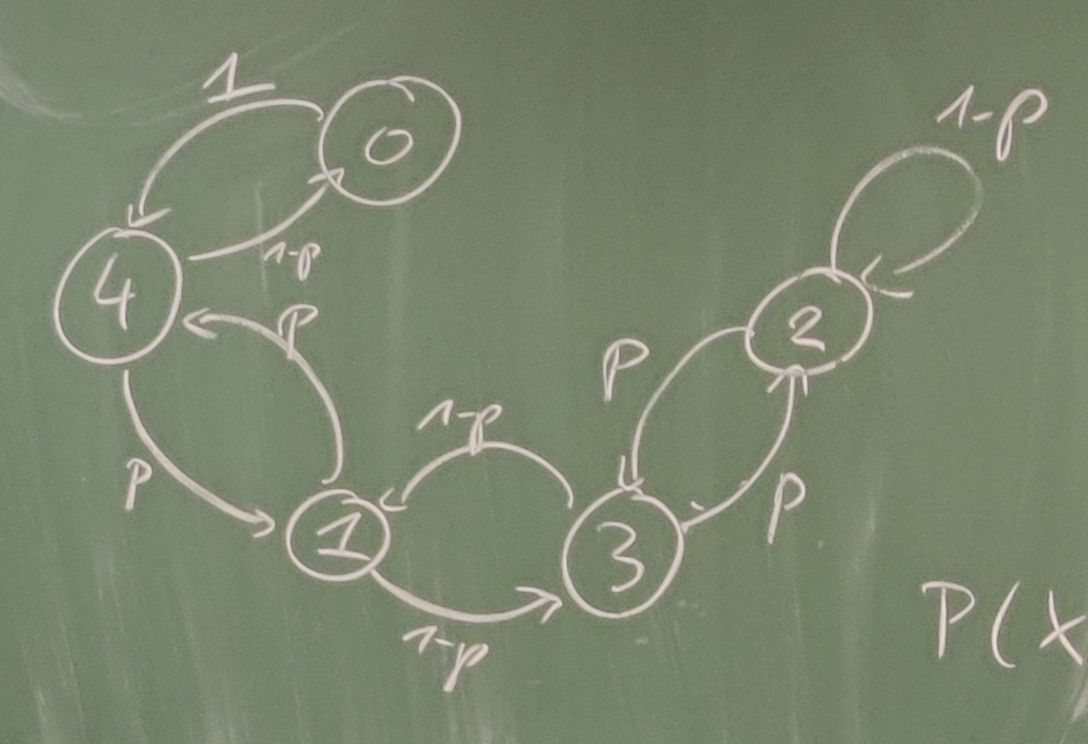
\includegraphics[width=0.7\textwidth]{tasks/02_markov.jpg} 
\end{center}

\textbf{Podpunkt 1.}
Jak widać, jest to łańcuch Markowa. Koniec.

A trochę dokładniejsze wytłumaczenie: 

Każdy z tych wierzchołków $(0), (1), (2), (3), (4)$ to liczba parasoli, które są w naszej lokalizacji. 
Czyli zaczynamy od stanu $(4)$ i jeśli nie pada deszcz, to nie bierzemy parasola i idziemy do biura w którym jest $4 - 4 = 0$ parasoli (stan $(0)$).
Jeśli natomiast pada deszcz, to bierzemy parasol i idziemy do biura w którym jest $4 - 4 + 1 = 1$ parasol (stan $(1)$).
Analogicznie dla innych stanów; jeśli jesteśmy w $(k)$ i pada, to bierzemy parasol i zwiększamy liczbę w tej drugiej lokazliacji (gdzie jest $4 - k + 1$ parasoli), a jeśli nie pada to nie bierzemy i jest $4 - k$ parasoli.

Dany stan zależy tylko od poprzedniego, bo nie obchodzi nas, czy jesteśmy w domu, czy w biurze, tylko to ile mamy koło siebie parasoli.

\textbf{Podpunkt 2.}
Ma rozkład stacjonarny. Możemy to policzyć na dwa sposoby:

\textbf{Sposób 1.}

Aby znaleźć rozkład stacjonarny, musimy rozwiązać równanie $\pi P = \pi$, gdzie $P$ to macierz przejścia, a $\pi = (\pi_0, \pi_1, \pi_2, \pi_3, \pi_4)$ to wektor rozkładu stacjonarnego.

Macierz przejścia $P$ jest następująca:
\[
P = \begin{pmatrix}
 & \mathbf{0} & \mathbf{1} & \mathbf{2} & \mathbf{3} & \mathbf{4} \\
\mathbf{0} & 0 & 0 & 0 & 0 & 1 \\
\mathbf{1} & 0 & 0 & 0 & 1-p & p \\
\mathbf{2} & 0 & 0 & 1-p & p & 0 \\
\mathbf{3} & 0 & 1-p & p & 0 & 0 \\
\mathbf{4} & 1-p & p & 0 & 0 & 0
\end{pmatrix}
\]

Tak więc mnożymy wektor $\pi$ przez macierz $P$ i przyrównujemy do $\pi$:
\[
\begin{cases}
\pi_4(1-p) = \pi_0 \quad & (1) \\
\pi_3(1-p) + \pi_4 p = \pi_1 \quad & (2) \\
\pi_2(1-p) + \pi_3 p = \pi_2 \quad & (3) \\
\pi_1(1-p) + \pi_2 p = \pi_3 \quad & (4) \\
\pi_0 + \pi_1 p = \pi_4 \quad & (5) \\
\sum_{k=0}^{4} \pi_k = 1 \quad & (6)
\end{cases}
\]

Z równania (3) otrzymujemy $\pi_2(1 - (1-p)) = \pi_3 p \implies \pi_2 = \pi_3$.
Podstawiając to do (4) mamy $\pi_1(1-p) + \pi_2 p = \pi_2 \implies \pi_1 = \pi_2$.
Następnie z (2), wiedząc że $\pi_3 = \pi_1$, mamy $\pi_1(1-p) + \pi_4 p = \pi_1 \implies \pi_4 = \pi_1$.

Mamy więc równość stanów: $\pi_1 = \pi_2 = \pi_3 = \pi_4$.
Z równania (1) wyznaczamy $\pi_0$: $\pi_0 = (1 - p)\pi_4$.

Podstawiamy do warunku sumowania (6):
\[
(1-p)\pi_4 + 4\pi_4 = 1 \implies \pi_4(1 - p + 4) = 1 \implies \pi_4 = \frac{1}{5 - p}
\]

Ostatecznie:
\[
\pi_0 = \frac{1 - p}{5 - p}, \quad \pi_1 = \pi_2 = \pi_3 = \pi_4 = \frac{1}{5 - p}
\]

\textbf{Sposób 2.} (ten nieszczęsny)

Skorzystamy z \href{https://en.wikipedia.org/wiki/Balance\_equation}{Global balance equation}.

Dla dowolnego podzbioru stanów $X \subset S$:

$$\underbrace{\sum_{x \in X} \left( \pi_x \sum_{y \notin X} p_{xy}\right)}_{\text{Wypływ z } X} = \underbrace{\sum_{y \notin X} \left( \pi_y \sum_{x \in X} p_{yx}\right)}_{\text{Wpływ do } X}$$

$$ \iff \pi \text{ jest rozkładem stacjonarnym}$$ 

Zauważmy jednak, że nie musimy sprawdzać wszystkich podzbiorów \(S\).
Jeśli sprawdzimy tylko singletony, to wystarczy, ponieważ dla dowolnego podzbioru \(X\) możemy rozbić sumę na sumy po singletonach.

Jeszcze tylko przypomnijmy, że \(p_{xy}\) to prawdopodobieństwo przejścia ze stanu \(x\) do stanu \(y\)
(nie pamiętam, czy na wykładzie było tak, czy na odwrót?).

Sprawdzamy więc dla każdego stanu:
Sprawdzamy więc bilans przepływu (wychodzące poza stan = wchodzące spoza stanu) dla każdego stanu:
\begin{enumerate}
    \item Dla $X = \{0\}$: $\pi_0 \cdot (1) = \pi_4 \cdot (1 - p)$
    \item Dla $X = \{1\}$: $\pi_1 \cdot (1) = \pi_3 \cdot (1 - p) + \pi_4 \cdot p$
    \item Dla $X = \{2\}$: $\pi_2 \cdot p = \pi_3 \cdot p$ \quad (nie liczymy po żadnej stronie 2 $\rightarrow$ 2 !)
    \item Dla $X = \{3\}$: $\pi_3 \cdot (1) = \pi_1 \cdot (1 - p) + \pi_2 \cdot p$
    \item Dla $X = \{4\}$: $\pi_4 \cdot (1) = \pi_0 \cdot (1) + \pi_1 \cdot p$
\end{enumerate}

Podobnie jak w Sposobie 1, rozwiązując te równania wraz z warunkiem sumowania, otrzymujemy ten sam rozkład stacjonarny.

\textbf{Podpunkt 3.}
Zdarzenie $A_n$ zachodzi, gdy pada deszcz i nie mamy parasola w domu lub w biurze.

Trzeba pamiętać, że dzień składa się z dwóch wyjść: z domu do biura i z biura do domu!

Czyli $A_n = \{(X_{2n} = 0 \land \text{ pada }) \lor (X_{2n+1} = 0 \land \text{ pada })\}$

Zauważmy też, że te zdarzenia są rozłączne. 
Jest tak, ponieważ liczba parasoli w domu i w biurze sumuje się do 4, więc jeśli zmoknę rano, to nie zmoknę po południu nawet jak będzie padać deszcz.
Zatem:  
\begin{align*}
    P(A_n) &= P(X_{2n} = 0 \land \text{ pada}) + P(X_{2n+1} = 0 \land \text{ pada}) \\
    &= p \cdot \pi_0 + p \cdot \pi_0 = 2p \pi_0 \text{ , dla n } \to \infty
\end{align*}

Czemu $p \cdot \pi_0$? Bo liczymy granicę, a po długim czasie zawsze rozkład zbliża się do rozkładu stacjonarnego.
Natomiast w stanie stacjonarnym $P(X_n = k) = \pi_k$ dla każdego $n$.


\[
\lim_{n \to \infty} P(A_n) = 2 \cdot (p \cdot \pi_0) = \frac{2p(1 - p)}{5 - p}
\]


\textbf{Podpunkt 4.}

Uogólniamy wzór na $\pi$ dla $N$ parasoli. 

Zauważmy, że do stanu \((0)\) możemy przejść tylko ze stanu \((N)\) gdy nie pada, tak więc \[\pi_0 = (1-p)\pi_N\]

Możemy udowodnić też, że dla takiego \(\pi_0\) oraz \(\pi_1 = \pi_2 = \ldots = \pi_N = x\), $\pi$ jest rozkładem stacjonarnym. Wystarczy skorzystać z global balance equation dla singletonów, podobnie jak w Podpunkcie 2:

Dla każdego \(k \in \{1, 2, \ldots, N-1\}\)
rozważamy stan \(X = \{k\}\): 
\[\pi_k = \pi_{N - k} \cdot (1 - p) + \pi _{N - k + 1} \cdot p\]
\[x = x \cdot (1 - p) + x \cdot p\]
\[x = x \text{ co jest prawdziwe}\]
Tak więc dla każdego \(k\) od 1 do \(N-1\) równanie jest spełnione.
Dla \(k = 0\) mamy już udowodnione, a dla \(k = N\) rozważamy stan \(X = \{N\}\):
\[\pi_N = \pi_0 + \pi_1 \cdot p\]
\[x = (1 - p)x + x \cdot p\]
\[x = x \text{ co jest prawdziwe}\]

Tak więc jest to rzeczywiście poprawny rozkład stacjonarny. 
Wiemy, że sumuje się do 1, więc możemy wyznaczyć \(x\):
\[(1 - p)x + N \cdot x = 1\]
\[x = \frac{1}{N + 1 - p}\]

Dzięki temu możemy policzyć ogólny wzór na prawdopodobieństwo zmoknięcia w ciągu dnia:
\[
P(A_n) = \frac{2p(1 - p)}{N + 1 - p}
\]

Dla Szkocji ($p = 0.6$) szukamy $N$, aby wynik był $< 0.1$:

\[
\frac{2 \cdot 0.6 \cdot 0.4}{N + 0.4} < 0.1
\]
\[
\frac{0.48}{N + 0.4} < 0.1 \quad \Big| \cdot 10(N+0.4)
\]
\[
4.8 < N + 0.4
\]
\[
N > 4.4
\]

Najmniejszą liczbą naturalną jest $N = 5$.

\subsection*{Odpowiedź}
\[
\boxed{\begin{aligned}
\text{(1)} & \quad \text{Tak, jest to łańcuch Markowa.} \\
\text{(2)} & \quad \text{Tak; } \pi = \left(\frac{1 - p}{5 - p}, \frac{1}{5 - p}, \frac{1}{5 - p}, \frac{1}{5 - p}, \frac{1}{5 - p}\right) \\
\text{(3)} & \quad \lim_{n \to \infty} P(A_n) = \frac{2p(1 - p)}{5 - p} \\
\text{(4)} & \quad 5 \text{ parasoli}
\end{aligned}}
\]
\section{Zadanie 3}
Udowodnij, że jeżeli jeden ze stanów w danej klasie relacji skomunikowania
jest stanem powracającym, to wszystkie stany w tej klasie są powracające.
\subsection*{Rozwiązanie}
Tak naprawdę cała intuicja jest taka że, skoro rozpatrujemy daną klasę skomunikowania to zachodzi: $\forall_{i,j} i\leftarrow j \text{ oraz } j\leftarrow i$. Załóżmy że wiemy, że stanem powracającym jest $i$. Teraz skoro to jest klasa skomunikowania to jak weźmiemy jakiś stan $x$ to zachodzi $i\leftarrow x$, ale ze względu na klasę skomunikowania zachodzi również $x\leftarrow i$. Zatem zauważmy że skoro istnieje ścieżka z $i$ do $i$ przez $x$ oraz $i$ jest powracający to $x$ też jest powracający.\\
Bardziej formalnie:\\

Jeśli $i$ i $j$ są w tej samej klasie komunikacji i stan $i$ jest powracający,
to stan $j$ również jest powracający.
\par
Ponieważ $i \leftrightarrow j$, istnieją liczby całkowite $n_0,m_0 \ge 1$
takie, że
\[
p_{j i}(n_0) > 0
\qquad\text{oraz}\qquad
p_{i j}(m_0) > 0 .
\]

Założenie, że stan $i$ jest powracający oznacza, że
\[
\sum_{r=0}^{\infty} p_{ii}(r) = +\infty.
\]

Dla każdego $r \ge 0$ zachodzi
\[
p_{j j}(n_0 + r + m_0)
\;\ge\;
p_{j i}(n_0) \, p_{i i}(r) \, p_{i j}(m_0).
\]

Sumując obie strony po wszystkich $r \ge 0$ otrzymujemy
\[
\sum_{t = 0}^{\infty} p_{j j}(t)
\;\ge\;
p_{j i}(n_0) \, p_{i j}(m_0)
\sum_{r = 0}^{\infty} p_{i i}(r).
\]

Ponieważ $p_{ji}(n_0) > 0$, $p_{ij}(m_0) > 0$ oraz
$\sum_{r=0}^{\infty} p_{ii}(r) = +\infty$, prawa strona sumy jest równa
$+\infty$. Zatem
\[
\sum_{t=0}^{\infty} p_{jj}(t) = +\infty,
\]
co oznacza, że stan $j$ jest powracający.

Wynika stąd, że każdy stan w klasie komunikacji, która zawiera stan powracający,
również jest powracający.

\section{Zadanie 4}
Udowodnij, że wskończonym łańcuchu Markova każdu stan powracający jest dodatni.

\subsection*{Dowód}
Niech \(S\) będzie przestrzenią stanów łańcucha Markowa, przy czym \(|S| < \infty\) (przestrzeń jest skończona).
Rozważmy stan powracający \(i \in S\). Niech \(C\) będzie klasą komunikacji, do której należy stan \(i\).

Z własności łańcuchów Markowa wiemy, że:
\begin{enumerate}
	\item Klasa \(C\) jest zamknięta (prawdopodobieństwo wyjścia z niej wynosi 0).
	\item Wszystkie stany w klasie \(C\) są powracające.
	\item Ponieważ cała przestrzeń \(S\) jest skończona, to \(C \subseteq S\) również jest zbiorem skończonym.
\end{enumerate}

Przeprowadzimy dowód nie wprost. \\
Załóżmy przeciwnie, że stan \(i\) (a zatem i wszystkie stany w klasie \(C\)) jest powracający zerowy.

Z definicji stanu powracającego zerowego wynika,
że granica prawdopodobieństw przejścia dąży do zera, czyli dla każdego \(j \in C\):
\[
	\lim_{n \to \infty} P_{ij}^{(n)} = 0
\]
gdzie \(P_{ij}^{(n)}\) oznacza prawdopodobieństwo przejścia ze stanu \(i\) do stanu \(j\) w \(n\) krokach.

Ponieważ klasa \(C\) jest zamknięta, w każdym kroku \(n\) suma prawdopodobieństw przejścia ze stanu \(i\) do wszystkich stanów tej klasy musi wynosić 1:
\[
	\sum_{j \in C} P_{ij}^{(n)} = 1
\]

Obłóżmy to granicą:
\[ \lim_{n \to \infty} \sum_{j \in C} P_{ij}^{(n)} = 1 \]

Ponieważ zbiór \(C\) jest skończony,
możemy zamienić kolejność sumowania i granicy (kluczowe)
\[ \sum_{j \in C} \left( \lim_{n \to \infty} P_{ij}^{(n)} \right) = 1 \]

Korzystając z naszego założenia podstawiamy \(0\) w miejsce granicy:
\[ \sum_{j \in C} 0 = 1 \]

Otrzymaliśmy sprzeczność
Zatem, stan \(i\) musi być powracający dodatni. \ \  \(\square\)

\section{Zadanie 5}
\autor{Filip Manijak}
Rozważmy dowolny (skończony lub nieskończony) łańcuch Markowa \((X_n)_{n \geq 0}\) w którym wszystkie stany są w tej samej klasie skomunikowania. Udowodnij, że jeżeli jeden ze stanów jest powracający dodatni, to wszystkie stany są powracające dodatnie.

\subsection*{Rozwiązanie}
Oznaczmy \(x\) jako stan, który jest powracający dodatni. Wtedy zauważmy, że dla każdego innego stanu \(y\):
\[E[T_{y,y}] \leq E[T_{y,x}]+ \sum T_{x,x}*k*(1-p_{y,x})^{k-1}p_{y,x}+E[x\xrightarrow{}y] =  E[T_{y,x}]+T_{x,x}(1/p_{x,y})+E[x\xrightarrow{} y]\]
Ten wzór to wartość oczekiwana rozkładu geometrycznego. \(C\) to taka liczba, żeby \(p_{x,y} >0\). Czyli twierdzę, że wartość oczekiwana kroków do powrotu jest mniejsza niż suma wartości oczekiwanych: Dojścia do stanu powracającego (to musi byś skończone, bo prawdopodobieństwo przejścia od x do y jest niezerowe), Wracania do stanu powracającego, tak długo aż nie wylosujemy powrotu do naszego punktu i powrotu do tego punktu. Jak widac prawa strona jest skończona.

\section{Zadanie 6}
\autor{Mateusz Wojaczek}
Udowodnij, że dla dowolnego skończonego nieprzywiedlnego łańcucha Markowa
istnieją stałe \(c > 0\), \(0 < \delta < 1\) takie, że dla każdego stanu \(z\) i dla każdego \(m \in \mathbb{N}_1\) mamy:
\[
	\mathbb{P}(T_z > m) \leq c \, \delta^m.
\]

\subsection*{Rozwiązanie}
Udowodnij, że dla dowolnego skończonego nieprzywiedlnego łańcucha Markowa
istnieją stałe \(c > 0\), \(0 < \delta < 1\) takie, że dla każdego stanu \(z\) i dla każdego \(m \in \mathbb{N}_1\) mamy:
\[
	\mathbb{P}(T_z > m) \leq c \, \delta^m.
\]

\textbf{Dowód.}
Z nieprzywiedlności i nieokresowości (korzystam z tego założenia bo Krystian pozwolił) łańcucha Markowa otrzymujemy, że istnieje \(N \in \mathbb{N}\) takie, że:
\[
	\forall n \geq N, \quad \forall x, y \quad P_{x,y}(n) > 0.
\]
W szczególności:
\[
	0 < a := \min_{x,y} P_{x,y}(N).
\]

Rozważmy teraz:
\[
	\mathbb{P}(T_z > m)
	= \mathbb{P}(X_0 \neq z, X_1 \neq z, \dots, X_m \neq z)
	\leq \mathbb{P}(X_0 \neq z, X_N \neq z, X_{2N} \neq z, \dots, X_{\lfloor m/N \rfloor N} \neq z).
\]
A zatem:
\[
	\mathbb{P}(T_z > m) \leq (1 - a)^{\lfloor m/N \rfloor}
	\leq (1 - a)^{\frac{m}{N} - 1}
	= \frac{1}{1-a} \left( (1 - a)^{1/N} \right)^m.
\]

Zatem otrzymujemy dokładnie poszukiwaną postać:
\[
	\mathbb{P}(T_z > m) \leq c \, \delta^m,
\]
gdzie:
\[
	c = \frac{1}{1-a}, \qquad \delta = (1-a)^{1/N}.
\]

\section{Zadanie 7}
\label{set07.task7}

tutaj wpisz treść zadania

\subsection*{Rozwiązanie}
tutaj wpisz rozwiązanie

\subsection*{Odpowiedź}
\[
\boxed{\text{tutaj daj odpowiedz}}
\]

\section{Zadanie 8 (Oskar Prusik)}
Udowodnij, że jeżeli x jest stanem istotnym i y jest osiągalny z x, to y jest stanem istotnym.

\subsection*{Rozwiązanie}
\paragraph{Definicje.} 

Z definicji nieistotności mamy:
\[
\text{nieistotny}(i) \;:=\; \exists j : (i \to j) \land (j \not\to i),
\]
zatem:
\[
\text{istotny}(i) \;\equiv\; \forall j : \big[ (i \not\to j) \;\lor\; (j \to i) \big].
\]

\paragraph{Założenia.} 
\begin{itemize}
	\item $x$ istotny: $\forall z \; \big[ (x \not\to z) \;\lor\; (z \to x) \big]$
	\item $x \to y$
\end{itemize}

\paragraph{Teza.}
$y$ istotny: $\forall w \; \big[ (y \not\to w) \;\lor\; (w \to y) \big]$.

\paragraph{Dowód.}
Weźmy dowolny stan $w$.

\underline{Przypadek 1:} $y \not\to w$. \\
Wtedy $ (y \not\to w) \lor (w \to y) $ jest prawdziwe.

\underline{Przypadek 2:} $y \to w$. \\
Z $x \to y$ i $y \to w$ wynika $x \to w$. \\
Z istotności $x$ dla $w$ mamy: $(x \not\to w) \lor (w \to x)$. \\
Skoro $x \to w$, to $(x \not\to w)$ jest fałszem, więc musi zachodzić $w \to x$.

Mamy $w \to x$ oraz $x \to y$, stąd $w \to y$. \\
Zatem $(w \to y)$ jest prawdą, więc alternatywa $(y \not\to w) \lor (w \to y)$ również.

W obu przypadkach formuła jest spełniona dla każdego $w$, co oznacza, że $y$ jest istotny. $\square$
\section{Zadanie 9}
Udowodnij, że w każdym skończonym łańcuchu Markowa istnieje przynajmniej jedna klasa komunikacji, w której wszystkie stany są istotne.

\subsection*{Rozwiązanie}

Popatrzmy sobie na skierowany graf przejść między stanami. Wiemy, że klasy komunikacji są silie spójnymi składowymi tego grafu. Rozważmy graf po skompresowaniu silnie spójnych składowych. Wiemy, że jest on DAGiem więc możemy go posortować topologicznie. Popatrzmy na ostatnią spójną składową po tym sortowaniu. Nie ma z niej żadnej krawędzi wychodzącej więc z każdego stanu który w niej jest możemy dojść tylko do wierzchołków z tej klasy i z każdego z nich możemy wrócić więc wszystkie stany w tej klasie są istotne.


\section{Zadanie 10 (Kacper Orszulak)}
Udowodnij, że jeżeli $\pi$ jest rozkładem stacjonarnym skończonego łańcucha Markowa o macierzy przejścia $P$, to $\pi_{y_0} = 0$ dla wszystkich nieistotnych stanów $y_0$.

\subsection*{Rozwiązanie}
$$
\begin{aligned}
    \pi &= \pi P \\
    \forall_{n \in \mathbb{N}} \; \pi &= \pi P^n \\
    \forall_{n \in \mathbb{N}} \; \pi_{y_0} &= \sum_{x \in S} \pi_x \mathcal{P}_{xy_0}(n) \\
    \sum_{n = 0}^\infty \pi_{y_0} &= \sum_{n = 0}^\infty \sum_{x \in S} \pi_x \mathcal{P}_{xy_0}(n) \\
\end{aligned}
$$
\begin{equation} \label{eq:1}
    \sum_{n = 0}^\infty \pi_{y_0} = \sum_{x \in S} \pi_x \sum_{n = 0}^\infty \mathcal{P}_{xy_0}(n) \\
\end{equation}

Pokażemy teraz, że $\forall_{x \in S} \; \sum_{n = 0}^\infty \mathcal{P}_{xy_0}(n) < \infty$.

Niech $N := |\{n \ge 0 \; | \; X_n = y_0\}| = $ liczba wizyt w $y_0$.

$$
\begin{aligned}
    \sum_{n=0}^\infty \; \mathcal{P}_{xy_0}(n) &=
    \sum_{n=0}^\infty \; \mathcal{P}(X_n = y_0 \; | \; X_0 = x) \\
    &= \mathbb{E}[N \; | X_0 = x] \\
    &= \sum_{n = 0}^\infty n \cdot \mathcal{P}(N = n \; | \; X_0 = x) \\
    &= \sum_{k = 1}^\infty \mathcal{P}(N \ge k \; | \; X_0 = x) \\
    &= \sum_{k = 1}^\infty \mathcal{P}_x(\text{liczba wizyt w $y_0$ co najmniej $k$ razy}) \\
    &= \sum_{k = 1}^\infty \mathcal{P}_x(\substack{\text{wizyta w } y_0 \\ \text{ po skończonej liczbie kroków}}) \cdot \mathcal{P}_{y_0}(\substack{\text{powrót do } y_0 \\ \text{po skończonej liczbie kroków}})^{k-1} \\
    &= \sum_{k = 1}^\infty \underbrace{\mathcal{P}_x(\tau_{y_0}^+ < \infty)}_{a} \cdot {\underbrace{\mathcal{P}_{y_0}(\tau_{y_0}^+ < \infty)}_{q}}^{k-1} \\
\end{aligned}
$$

Korzystając z \hyperref[set07.task7]{zadania 7.}, wiemy iż $q < 1$. Dany szereg jest zatem zbieżny:
$$
    \sum_{k=1}^\infty a \cdot q^{k-1} = \frac{p}{q-1} < \infty
$$

Pokazaliśmy zatem, że $RHS$ równania \eqref{eq:1} jest skończone. Lewa strona zatem też musi być skończona. LHS to nieskończona suma pewnej stałej, zatem ta stała musi być zero. Dokładniej $\pi_{y_0} = 0$. \hfill $\square$

\section{Zadanie 11}
\label{set07.task11}
Udowodnij, że jeżeli macierz przejścia $P$ jest symetryczna ($p_{x,y}=p_{y,x}$), to rozkład jednostajny jest rozkładem stacjonarnym dla $P$.

\subsection*{Rozwiązanie}
Skorzystamy z ”ogólnej wskazówki” z zestawu:\\
Niech $P$ będzie macierzą przejścia łańcucha Markowa na zbiorze stanów $S$.
Niech $\pi$ będzie rozkładem prawdopodobieństwa na $S$.
Łatwo uzasadnić, że jeśli dla każdego $x,y\in S$ mamy
\[
\pi_x p_{x,y} = \pi_y p_{y,x}
\]
to $\pi$ jest rozkładem stacjonarnym.

Zauważmy, że $\pi$ – rozkład stacjonarny ($\forall x,y\in S\ \pi_x=\pi_y$) w połączeniu z symetrią
macierzy $P$ implikuje równość, o której mowa we wskazówce: dla każdego $x,y\in S$, zatem rozkład jednostajny jest rozkładem stacjonarnym dla $P$. CKD


\section{Zadanie 12}
\autor{Aleksander Wieczorek}
Niech P będzie macierzą przejścia spaceru losowego na cyklu długości 2025.
Znajdź najmniejszą wartość \(t\) taką, że \(p_{x,y}(t) > 0\) dla wszystkich stanów x i y.
\subsection*{Rozwiązanie}
Zauważmy od razu, że nasz łańcuch jest nieokresowy. Z wierzchołka i krawędzią nieskierowana możemy się wrócić w 2 krokach,\footnote{zakładam, że między każdą parą sąsiednich wierzchołków da się przejść w obie strony. Gdyby tak nie było dużo ciężej przeanalizować problem, bo takie t mogłoby nie istnieć} albo przejść cały cykl w 2025 krokach, więc \[o(i)=gcd(2,2025)=1\] Cykl jest spójny, łańcuch jest nieprzywiedlny , więc każdy wierzchołek ma okres 1.\\
Stąd wynika, że istnieje takie t dla którego \(\forall_{x,y} p_{x,y}(t)>0\).\\
Dodatkowo zauważmy, że wybór punktu startowego x jest nieistotny - cykl można obrócić.\\
Jeśli przejdziemy jakąś ścieżkę w k krokach to możemy przejść nią w k+2 krokach dodając przejście krawędzią "tam i z powrotem".\\
Jedynym problemem przejścia między parą wierzchołko w t krokach jest parzystość t.\\
Dla każdego wierzchołka y \(dist(x,y)\) ma inną parzystość niż \(2025-dist(x,y)\), więc między każdą parą wierzchołków istnieje najkrótsza ścieżka o każdej parzystości.\\
Wystarczy ustalić najmniejsze t dla którego wszystkie takie ścieżki mają długość \(\le\) t.
\begin{itemize}
	\item Aby przejść z x do x w nieparzystą liczbę kroków musimy obejść cały cykl, który ma długość 2025, więc nieparzyste \(t<2025\) odpada
	\item Aby przejść z x do jego sąsiada w parzystą liczbę kroków musimy obejść prawie cały cykl, więc najkrótsza taka ścieżka ma długość 2024, więc parzyste \(t<2024\) również odpadają,
\end{itemize}
Uwzględniając oba warunki najmniejszą niewykluczoną odpowiedzią jest t=2024.
\subsection*{Odpowiedź}
\[
	\boxed{\text{2024}}
\]

\section{Zadanie 13}
\autor{Dominik Korsa}
Niech \(G\) będzie skończonym grafem z co najmniej jedną krawędzią.
Rozważmy łańcuch Markowa, gdzie przestrzeń stanów \(\Omega(G)\) jest rodziną
wszystkich zbiorów niezależnych w \(G\).
Krok ze stanu \(M_t\) do następnego stanu działa następująco.
Losujemy jednostajnie \(v \in V(G)\).
Jeśli \(v \in M_t\) to \(M_{t+1} = M_t \setminus \{v\}\).
Jeśli \(v \notin M_t\) to próbujemy dodać \(v\) do \(M_t\).
To znaczy, jeśli \(M_t \cup \{v\}\) jest zbiorem niezależnym w \(G\)
to \(M_{t+1} = M_t \cup \{v\}\), a w przeciwnym przypadku \(M_{t+1} = M_t\).
Udowodnij, że ten łańcuch jest nieprzywiedlny, nieokresowy i jego rozkład
stacjonarny jest jednostajny.

\subsection*{Rozwiązanie}
Niech \(n = |V(G)|\).

\subsubsection*{Nieprzywiedlność}
Aby udowodnić nieprzywiedlność tego łańcucha musimy udowodnić, że wszystkie
pary stanów (zbiorów niezależnych w \(G\)) się wzajemnie komunikują,
czyli dla każdej pary zbiorów niezależnych \(A, B \subseteq V(G)\)
istnieje takie \(k\), że \(P_{A,\,B}(k) > 0\).

Niech \(A = \{a_1, a_2, \dots, a_l\}\) i \(B = \{b_1, b_2, \dots, b_m\}\)
to pewnie zbiory niezależne. Następujący skończony ciąg kroków przechodzi ze
stanu \(A\) do \(\emptyset\), a następnie do \(B\):
\begin{itemize}
  \item Usuń \(a_1\) ze zbioru \(A\). Taki krok jest możliwy, bo zbiór
  niezależny po usunięciu wierzchołka pozostaje niezależny, i ma
  prawdopodobieństwo \(n^{-1}\).
  \item Podobnie usuwaj wierzchołki \(a_2\) do \(a_l\). Po tych krokach jesteśmy
  w stanie \(\emptyset\).
  \item Dodaj \(b_1\) do stanu \(\emptyset\). Ten krok ma prawdopodobieństwo
  \(n^{-1}\)
  \item Podobnie dodawaj wierzchołki \(b_2, \dots, b_m\). Każdy z takich kroków
  jest możliwy, bo wszystkie stany są podzbiorami zbioru niezależnego \(B\),
  więc również są zbiorami niezależnymi.
\end{itemize}
Zatem te \(k+l\) kroków, każde o prawdopodobieństwie \(\frac{1}{n}\) wystarcza,
aby przejść ze stanu \(A\) do \(B\), więc \(P_{A,\,B}(l+m) \geq n^{-(l+m)} > 0\).

\subsubsection*{Nieokresowość}
Niech \(A\) to maksymalny ze względu na inkluzję zbiór niezależny w \(G\).
Z treści zadania w \(G\) istnieje przynajmniej jedna krawędź, a skoro \(A\)
jest zbiorem niezależnym, to któryś z końców tej krawędzi, nazwijmy go \(v\),
nie należy do \(A\).

Będąc w stanie \(A\) wylosowanie wierzchołka \(v\) spowoduje pozostanie w
stanie \(A\) (z maksymalności \(A\)), więc: \(P_{A,\,A} \geq n^{-1} > 0\).

Definicja okresu stanu to
\(\operatorname{o}(v) = \gcd \mathcal{T}(v)\), gdzie
\(
  \mathcal{T}(v) = \{ t \in \mathbb{N}_1 \mid P_{v,\,v}(t) > 0 \}
\).\\
\(P_{A,\,A} = P_{A,\,A}(1) > 0\), więc \(1 \in \mathcal{T}(v)\), więc
\(\operatorname{o}(v) = 1\). Z lematu z wykładu:
\begin{quote}
  W nieprzywiedlnym łańcuchu Markowa wszystkie stany mają ten sam okres.
\end{quote}
W takim razie wszystkie stany mają okres \(1\), zatem łańcuch jest
\textbf{nieokresowy}.

\subsubsection*{Jednostajność rozkładu stacjonarnego}
Udowodnijmy, że macierz przejścia \(P\) łańcucha Markowa z zadania jest
symetryczna, czyli dla każdego \(A, B \in \Omega(G)\) zachodzi
\(P_{A,\,B} = P_{B,\,A}\).

\begin{itemize}
  \item Jeżeli \(A = B\) to \textbf{tr.}

  \item Jeżeli \(A\) różni się od \(B\) dokładnie jednym wierzchołkiem,
  powiedzmy \(B = A \cup \{v\}\), to jedynie wylosowanie \(v\)
  (z prawdopodobieństwem \(n^{-1}\)) przechodzi między tymi stanami.
  Skoro \(A\) i \(B\) są zbiorami niezależnymi, to ten krok się udaje.
  Zachodzi \(P_{A,\,B} = P_{B,\,A} = n^{-1}\).

  \item Jeżeli \(A\) różni się od \(B\) więcej niż jednym wierzchołkiem,
  to \(P_{A,\,B} = P_{B,\,A} = 0\), bo każdy krok dodaje lub usuwa co najwyżej
  jeden wierzchołek.
\end{itemize}

Z \hyperref[set07.task11]{zadania 11} wiemy, że skoro macierz przejścia
\(P\) jest symetryczna, to rozkład stacjonarny jest rozkładem jednostajnym.

\section{Zadanie 14}
Rozważ spacer losowy po grafie przedstawionym na rysunku.
Spacer startuje z wierzchołka A.
Rozważ stowarzyszony z nim łańcuch Markowa $(X_n)_{n\in \mathbb{N}}$,
gdzie stanami są wuerzchołki grafu oraz $X_0 = A$.
\begin{enumerate}[label=(\roman*)]
    \item\label{set07.task14.1} Wyznacz $\lim_{n\to\infty} P(X_n = A)$ oraz $\lim_{n\to\infty} P(X_n = B)$.
    \item\label{set07.task14.2} Jaka jest oczekiwana liczba odwiedzin wierzchołka B przed pierwszym powrotem do A?
\end{enumerate}
\begin{center}
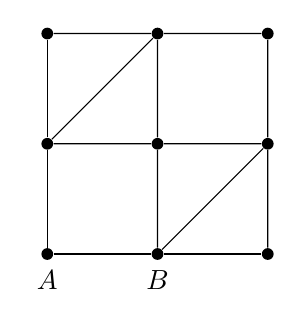
\begin{tikzpicture}[scale=1.4]

    % Wierzchołki
    \node (A) at (0,0) [circle,fill,inner sep=1.5pt,label=below:$A$] {};
    \node (B) at (1,0) [circle,fill,inner sep=1.5pt,label=below:$B$] {};
    \node (C) at (2,0) [circle,fill,inner sep=1.5pt] {};
    
    \node (D) at (0,1) [circle,fill,inner sep=1.5pt] {};
    \node (E) at (1,1) [circle,fill,inner sep=1.5pt] {};
    \node (F) at (2,1) [circle,fill,inner sep=1.5pt] {};
    
    \node (G) at (0,2) [circle,fill,inner sep=1.5pt] {};
    \node (H) at (1,2) [circle,fill,inner sep=1.5pt] {};
    \node (I) at (2,2) [circle,fill,inner sep=1.5pt] {};
    
    % Krawędzie poziome
    \draw (A) -- (B) -- (C);
    \draw (D) -- (E) -- (F);
    \draw (G) -- (H) -- (I);
    
    % Krawędzie pionowe
    \draw (A) -- (D) -- (G);
    \draw (B) -- (E) -- (H);
    \draw (C) -- (F) -- (I);
    
    % Przekątne
    \draw (D) -- (H); % górny lewy kwadrat
    \draw (B) -- (F); % dolny prawy kwadrat
    
\end{tikzpicture}
\end{center}

\subsection*{Rozwiązanie podpunktu \ref{set07.task14.1}}
Łańcuch jest skończony, spójny i aperiodyczny 
(w grafie są trójkąty i kwadraty, więc okres $= gcd(3, 4) = 1$) więc dla każdego puktu $Q$ 
$P(X_n = Q)$ zbiega do rozkładu stacjonarnego $\pi$.
Dla losowego spaceru po grafie rozkład stacjonarny ma postać:

\[
\pi(v)=\frac{\deg(v)}{\sum_{u}\deg(u)}.
\]

Wierzchołki narożne mają stopień $2$, pozostałe pięć
wierzchołków ma stopień $4$. Suma stopni:

\[
4\cdot 2 + 5\cdot 4 = 28.
\]

Więc

\[
\pi(A)=\frac{\deg(A)}{28}=\frac{2}{28}=\frac{1}{14}, 
\qquad
\pi(B)=\frac{\deg(B)}{28}=\frac{4}{28}=\frac{1}{7}.
\]

Czyli:

\[
\lim_{n\to\infty} P(X_n = A) = \frac{1}{14},
\qquad
\lim_{n\to\infty} P(X_n = B) = \frac{1}{7}.
\]

\subsection*{Rozwiązanie podpunktu \ref{set07.task14.2}}
Oczekiwana liczba odwiedzeń wierzchołka $B$ przed powrotem do $A$ to po prostu
stosunek średniej liczby odwiedzin $B$ do odwiedzin $A$ w długim czasie ($n\to\infty$), 
który jest równy:

\[
\frac{\pi(B)}{\pi(A)}
= \frac{1/7}{1/14}
= 2.
\]

\subsection*{Odpowiedź}
\[
\boxed{
    \text{(i)} 
        \lim_{n\to\infty} P(X_n = A) = \frac{1}{14},
        \qquad
        \lim_{n\to\infty} P(X_n = B) = \frac{1}{7}
        \qquad
    \text{(ii)} 
        \qquad 
        2
    }
\]

\section{Zadanie 15}
Niech $X_n$ będzie zmienną losową równą sumie oczek w $n$ niezależnych rzutach sprawiedliwą kostką. Pokaż, że dla każdego $k \in \mathbb{N}_2$ zachodzi
\[
\lim_{n \to \infty} P(X_n \text{ jest podzielne przez } k) = \frac{1}{k}.
\]

\subsection*{Rozwiązanie}

Oznaczmy $A_n$ - zmienną losową będącą liczbą oczek w $n$-tym rzucie.

Zauważmy, że:
\[
X_{n+1} \equiv X_n + A_{n+1} \pmod{k},
\]
więc $X_n$ tworzy łańcuch Markowa ze stanami będącymi resztami z dzielenia przez $k$.

Policzymy rozkład stacjonarny tego łańcucha.

Prawdopodobieństwo przejścia z dowolnego stanu $i$ do każdego z $i+1, i+2, \dots, i+6 \pmod{k}$ jest równe $\frac{1}{6}$. Macierz przejścia przyjmie więc postać:
\[
P =
\begin{bmatrix}
\frac{1}{6} & \frac{1}{6} & \frac{1}{6} & \frac{1}{6} & \frac{1}{6} & \frac{1}{6} & 0 & \cdots & 0\\[2ex]
0 & \frac{1}{6} & \frac{1}{6} & \frac{1}{6} & \frac{1}{6} & \frac{1}{6} & \frac{1}{6} & 0 & \cdots\\[2ex]
\vdots & & & & & & & & \vdots\\[2ex]
\frac{1}{6} & \frac{1}{6} & \frac{1}{6} & \frac{1}{6} & \frac{1}{6} & 0 & \cdots & 0 & \frac{1}{6}\\[2ex]
\frac{1}{6} & \frac{1}{6} & \frac{1}{6} & \frac{1}{6} & \frac{1}{6} & \frac{1}{6} & 0 & \cdots & 0
\end{bmatrix}.
\]

Równanie na rozkład stacjonarny $\pi$ przyjmuje postać:
\[
\pi = P \pi,
\]
czyli
\[
\begin{bmatrix}
\pi_0\\[1.5ex]
\pi_1\\[1.5ex]
\vdots\\[1.5ex]
\pi_{k-1}
\end{bmatrix}
=
\begin{bmatrix}
\frac{\pi_1+\pi_2+\pi_3+\pi_4+\pi_5+\pi_6}{6} \\[1.5ex]
\frac{\pi_2+\pi_3+\pi_4+\pi_5+\pi_6+\pi_7}{6} \\[1.5ex]
\vdots\\[1.5ex]
\frac{\pi_0+\pi_1+\pi_2+\pi_3+\pi_4+\pi_5}{6}
\end{bmatrix},
\quad
\text{oraz} \quad
\sum_{i=0}^{k-1} \pi_i = 1.
\]

Jasno widać, że rozwiązaniem tego układu jest:
\[
\pi_i = \frac{1}{k}, \quad i = 0,1,\dots,k-1.
\]

Z własności rozkładu stacjonarnego wynika więc:
\[
\lim_{n \to \infty} P(X_n \equiv i \pmod{k}) = \pi_i =  \frac{1}{k}.
\]

W szczególności:
\[
\lim_{n \to \infty} P(X_n \equiv 0 \pmod{k}) = \pi_0 = \frac{1}{k}.
\]
\section{Zadanie 16}

Mysz i kot niezależnie od siebie przemieszczają się w sposób losowy po
spójnym, nieskierowanym i niedwudzielnym grafie G.
Niech \(n\) = \( |V(G)|, m = |E(G)| \). Pokaż, że \(O(m^2n)\) jest
ograniczeniem górnym na oczekiwaną liczbę kroków, po której dojdzie do
spotkania.

\textit{Wskazówka: rozważ łańcuch Markowa na parach indeksów
	\((a, b)\)}

\subsection*{Rozwiązanie}

Oznaczmy wierzchołki i krawędzie naszego grafu \(V\) i \(E\)
(czyli \(G = (V, E)\)).

Zbudujemy graf \(H = (V_H, E_H)\), gdzie
\begin{itemize}
	\item \(V_H = V \times V\) - wierzchołek nowego grafu będzie parą
	      wierzchołków w oryginalnym grafie
	\item \(E_H = \big\{\{(u, v), (w, t)\} \in \binom{V_H}{2} \colon
	      \{u, w\} \in E \land \{v, t\} \in E
	      \big\}\)
	      \\- krawędź nowego grafu będzie oznaczała, że w grafie \(G\) były takie
	      dwie krawędzie, którymi można było przejść z jednej pary wierzchołków
	      do drugiej.
\end{itemize}
Zauważmy, że spacer losowy w grafie \(H\) jest tym samym co operacja
z treści zadania.
Załóżmy, że mysz i kot byli w wierzchołkach \(a\) i \(b\), a po
ruchu są w \(c\) i \(d\). Szansa na to w oryginalnym grafie to
\(\frac{1}{d(a)}\cdot\frac{1}{d(b)}\) (z definicji spaceru losowego).
\\W grafie
H oznacza to przejście z wierzchołka \((a, b)\) do \((c, d)\),
czyli szansa była \(\frac{1}{d_H((a,b))}\).\\
\(d_H((a, b))\) jest liczbą par wierzchołków, do których można się
dostać z pary \((a, b)\), czyli dokładnie \(d(a)\cdot d(b)\).\\
Prawdopodobieństwo tych dwóch zdarzeń jest identyczne.

Łatwo zauważyć, że \(|V_H| = |V| \cdot |V| = n^2\)\\
Trudniej \(|E_H| = \frac{1}{2} \sum_{a, b \in V} d(a)d(b)
= \frac{1}{2} \sum_{a \in V} d(a) \sum_{b \in V} d(b)
= \frac{1}{2} \cdot 2m \cdot 2m = 2m^2
\)

Znajdźmy w grafie \(G\) nieparzysty cykl \(c\)
(graf nie jest dwudzielny).

Załóżmy, że mysz zaczęła w wierzchołku \(x\), a kot w \(y\).

Niech \(p_1\) oznacza spacer (ścieżkę z możliwymi powtórzeniami)
długości \(n\) zaczynający się w \(x\) i kończący się w \(c\).
Taki spacer oczywiście istnieje. W grafie spójnym w co najwyżej
\(n-1\) krokach można się dostać do dowolnego wierzchołka,
a następnie można krążyć wokół cyklu.

Analogicznie niech \(p_2\) oznacza spacer z \(x\) do dowolnego
punktu na \(c\), długości dokładnie \(n\).

Teraz kontynuujmy spacery \(p_1\) i \(p_2\) równocześnie w
przeciwnych kierunkach wokół cyklu. Po co najwyżej
\( |c| \leq n \) krokach spacery spotkają się
(bo \(c\) miał nieparzystą długość)

Znaleźliśmy dwa spacery o równej długości, nie większej niż \(2n\),
które kończą się w tym samym punkcie.
Te dwa spacery w grafie \(G\) możemy potraktować jako jeden spacer w
grafie \(H\), zaczynający się w wierzchołku \((x, y) \in V_H\), a
kończący się w jakimś \((z, z)\). Oznaczmy go \(p\).

Skorzystamy z lematu z ćwiczeń (\texttt{Lemma 7.14}):
Dla krawędzi \((u, v)\) mamy \(h_{u, v} + h_{v, u} \leq 2|E|\),
gdzie \(h_{u, v}\) to oczekiwany czas osiągnięcia wierzchołka \(v\)
zaczynając w \(u\).\\
Nam wystarczy \(h_{u, v} \leq 2|E|\).

Będziemy iterować się po krawędziach na ścieżce \(p\) w grafie \(H\).
Oczekiwany czas przejścia jedną krawędzią jest z lematu
co najwyżej \(2|E_H|\), a krawędzi jest co najwyżej \(2n\).

\[
	\ev{\texttt{liczba kroków}} \leq |p| \cdot 2|E_H|
	\leq 2n \cdot 2 \cdot 2m^2 = 8m^2n = O(m^2n)
	\quad \square
\]

\section{Zadanie 17}
Rozważmy cykl na $n$ wierzchołkach. Startujemy w dowolnym wierzchołku. W każdym kroku z równym prawdopodobieństwem przechodzimy do jednego z sąsiadów. Jaka jest(asymptotycznie względem $n$) wartość oczekiwana liczby kroków do odwiedzenia wszystkich wierzchołków cyklu? \\
\\
(i) Ograniczenie górne\\
(ii) Ograniczenie dolne\\
(iii) A co jeżeli w każdym kroku z równym prawdopodobieństwem, czyli $\frac{1}{3}$, zostajemy lub przechodzimy do jednego z sąsiadów?

\subsection*{Rozwiązanie}
Skorzystamy z następujących lematów z książki dla spacerów losowych w grafie $G$:\\
\\
\textbf{Lemat 7.14.}
Dla $u,v \in E(G)$ oczekiwany czas przejścia z $u$ do $v$ i z powrotem do $u$ wynosi $h_{u,v} + h_{v,u} \leq 2|E(G)|$
\\
\textbf{Lemat 7.15.}
Czas pokrycia w grafie $G$ jest ograniczony z góry przez $2|E|(|V|-1)$.
\\

Przez $X$ będziemy oznaczać liczbę kroków potrzebną do odwiedzenia wszystkich wierzchołków.

\textbf{(i)} Z lematu 7.15. mamy oszacowanie z góry: $E(X) \leq 2|E|(|V|-1) = 2\cdot 2n\cdot (n-1) = O(n^2)$


\textbf{(ii)}
Możemy skorzystać z faktu, że w spacerze z dwoma barierami pochłaniającymi, 0 i $n$, oczekiwana liczba kroków do uderzenia w barierę startując z $k$ wynosi $k(n-k)$(można to pokazać indukcyjnie po wyprowadzeniu wzoru)

Oznaczmy $X_i$ - oczekiwana liczba kroków od momentu odwiedzenia po raz pierwszy $(i-1)$-ego z kolei wierzchołka do odwiedzenia po raz pierwszy $i$-tego wierzchołka. Oczywiście $X_1$ = 0, i zauważmy, że $X = X_1 + ... + X_n$. Jednak $X_i$ możemy rozpatrywać jako właśnie oczekiwaną liczbę kroków w spacerze losowym o barierach w 0 oraz $i$, ponieważ wszystkie odwiedzone dotychczas wierzchołki sąsiadują ze sobą, tworząc ścieżkę długości $i-1$, a ostatni odwiedzony jest jednym z jej końców(wynika ze sposobu w jaki spacerujemy po grafie) - czyli stoimy na polu 1 albo $i-1$ na tej ścieżce z barierami. Wobec tego $E(X_i) = (i-1)\cdot 1 = i-1$.

$E(X) = E(X_1 + ... + X_n) = E(X_1) + ...+E(X_n) = \sum_{i = 1}^n (i-1) = O(n^2)$


\textbf{(iii)} Oznaczmy oczekiwaną liczbę kroków z takim rozkładem prawdopodobieństwa jako $E(X')$ Zauważmy że $E(X') = \frac{3}{2}E(X)$, a skoro $E(X) = O(n^2)$ to $E(X') = O(n^2)$
\subsection*{Odpowiedź}
\[
\boxed{\text{W każdym z podpunktów } O(n^2)}
\]

\section{Zadanie 18}
Graf $L_n$ nazywamy lizakiem i zdefiniowany jest następująco (niech $n$ będzie parzyste). Wierzchołki $\{1, ... , n/2\}$ tworzą klikę $K_{n/2}$, niech $u$ będzie jednym z wierzhołków tej kliki. Pozostałe $n/2$ w połączeniu z $u$ tworzą ściężkę indukowaną na $n/2+1$ wierzchołkach. Niech $v$ będzie najbardziej odległym od kliki wierzchołkiem należącym do ścieżki (jedyny wierzchołek w lizaku o stopniu 1). Pokaż, że oczekiwany czas odwiedzenia wszystkich wierzcołków lizaka podczas spaceru wynosi:

(I) $\theta (n^2)$, przy założeniu, że startujemy w $v$.

(II) $\theta (n^3)$, przy założeniu, że startujemy w $u$.

\subsection*{Rozwiązanie}

Info na start, w dalszych rozważań, nie będę uwzględniał stałych prz n, więc na przykład, pomimo, że klika ma rozmiar $\frac{n}{2}$, to bedę mówił, że ma rozmiar $n$. Ponieważ, intersuję nas tylko $\theta$, to można tak zrobić.

(I) Podzielmy sobie problem, na przejście z $v$ do $u$, a potem zrobienie pozostałych wierzchołków z kliki zaczynając z $u$.

Przejście z $v$ do $u$, możemy traktować jako jako spacer losowy z dwoma barierami. Najpierw idziemy do sąsiada $v$, a potem z prawdopodobieństwiem $\frac{1}{n}$, pójścia do $u$. Oznacza, to, że oczekujemy, że $n$ razy wrócimy do $v$, zanim dojdziemy do $u$. Ponieważ każdy spacer ma oczekiwaną liczbę ruchów równą $n$, to oczekiwana liczba ruchów z dojścia z $v$ do $u$ to $n * n = n^2$.

Teraz zauważamy, że chodzenie po klice, by zaliczyć wszystkie wierzchołki, jest izomorficzne z problemem kolekcjonera kuponów. (Tutaj z gwazdką, ponieważ, nie ma szansy na powrót do tego samego kuponu, ale to tylko polepsza złożoność, a pesymistyczną $n^2$, dostaliśmy już wcześniej). Wiemy, że potrzbujemy w oczekiwaniu $n log n$ ruchów, by zaliczyć wszystkie wierzchołki.

Tutaj warto dodać jeszcze jedną stało. Za każdym razme, kiedy robimy coś coś w kolekcjonerze kuponów, jest szansa, że będąc w $u$ przejdziemy na ścieżkę. Będąc w $u$ ta szansa, żeby przejść na ścieżkę to $\frac{1}{n}$, natomiast, łatwo zauważyć, że po pewnym szansie szansa, że w kuponach będziemy w $u$ to też $\frac{1}{n}$. Wiec możemy powiedzieć, że prawdopodobieństwo wejścia na ścieżkę  jest równe $\frac{1}{n^2}$, co daje nam oczekiwaną liczbę pójść na ścieżkę jako stałą, o na lepszej expected wartości niż przejście z $v$ do $u$.

Suma kosztów wychodzi $\theta(n^2)$

(II) Teraz zobaczmy co się dzieje jeśli zaczynamy od $u$. W klicę to nadal oczekiwana wartośc ruchów to $n*log(n)$.

Natomiast ciekawsze jest jaka jest szansa na dojście do $v$. Wejście na ścieżkę ma prawdopodobieństwo $\frac{1}{n^2}$ (wyżej opisane). Żeby dojść do $v$ szansa jest $\frac{1}{n}$ (symetryczność z przypadkiem $v->u$). Więc potrzebujemy $n^3$ ruchów w klice i $n$ razy pójścia po ścieżce(gdzie każde przejście kosztuje $n$ ruchów). 

$n^3$ ruchów w klidze majoryzuje wsyztskie pozostałe wydatki ruchów, więc koszt ruchów, przed oczekianych odwiedzeniem wszystkch wierzchołków to $n^3$.


\section{Zadanie 19}
\begin{figure}[h!]
	\centering
	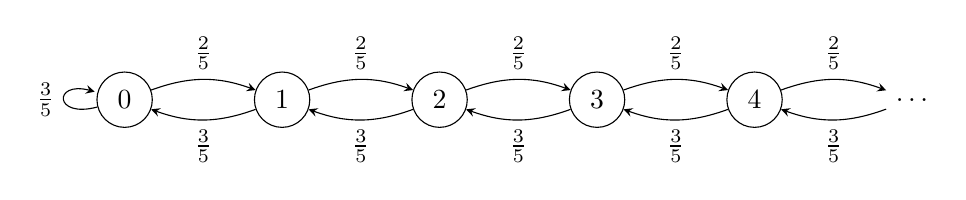
\begin{tikzpicture}[>=stealth, node distance=2cm, auto]
		\tikzstyle{state}=[circle, draw, minimum size=20pt]

		% nodes
		\node[state] (0) {0};
		\node[state, right of=0] (1) {1};
		\node[state, right of=1] (2) {2};
		\node[state, right of=2] (3) {3};
		\node[state, right of=3] (4) {4};

		% self-loop at 0
		\path[->] (0) edge[loop left] node {$\frac{3}{5}$} ();

		% transitions
		\path[->] (0) edge[bend left=20] node {$\frac{2}{5}$} (1);
		\path[->] (1) edge[bend left=20] node {$\frac{3}{5}$} (0);

		\path[->] (1) edge[bend left=20] node {$\frac{2}{5}$} (2);
		\path[->] (2) edge[bend left=20] node {$\frac{3}{5}$} (1);

		\path[->] (2) edge[bend left=20] node {$\frac{2}{5}$} (3);
		\path[->] (3) edge[bend left=20] node {$\frac{3}{5}$} (2);

		\path[->] (3) edge[bend left=20] node {$\frac{2}{5}$} (4);
		\path[->] (4) edge[bend left=20] node {$\frac{3}{5}$} (3);

		\node[,right of=4] (5) {$\dots$};

		\path[->] (4) edge[bend left=20] node {$\frac{2}{5}$} (5);
		\path[->] (5) edge[bend left=20] node {$\frac{3}{5}$} (4);

	\end{tikzpicture}
\end{figure}


Czy zadany wyżej spacer \(\Gamma\) jest nieprzywiedlnym i nieokresowym
łańcuchem Markowa? Czy istnieje jego rozkład stacjonarny?
Na podstawie poprzednich wniosków wywnioskuj,
jaką wartość przyjmuje \(\ev{\tau_x^{+}}\).


\subsection*{Rozwiązanie}

Łańcuch \(\Gamma\) jest nieprzywiedlny bo z każdego stanu możemy dojść do każdego. Jest też nieokresowy bo okres \(0\) jest równy \(1\) (da się dojść z \(0\) do \(0\)  w 1 kroku więc gcd równa się \(1\)), a jako iż jest nieprzywiedlny to okres wszystkich stanów jest identyczny.\\

Chcemy znaleść rozkład stacjonarny \(\pi\). Z definicji rozkładu stacjonarnego mamy, że:\\
\(\pi_0 = \pi_0 \cdot P(0,0) + \pi_1 \cdot P(1,0) = \pi_0 \cdot \frac{2}{5} + \pi_1 \cdot \frac{3}{5}  \implies \pi_1 = \frac{2}{3} \pi_0\)\\

Dla \(i>1\): \\
\(\pi_i = \pi_{i-1} \cdot P(i-1,i) + \pi_{i-1} \cdot P(i+1, i) = \pi_{i-1} \cdot \frac{2}{5}+ \pi_{i-1} \cdot \frac{3}{5}\)

Z tego równania, można się domyśleć, że jak coś ma je spełniać to coś w postaci \(\pi_i =\pi_0 \cdot r^i\). Jak podstawimy \(\pi_i = \pi_0 (\frac{2}{3} ) ^i\) co sugeruje nam to pierwsze równanie to okazuje się że drugie też jest spełnione. Pozostaje policzyć \(\sum_{i = 0}^{i=\infty} \pi_i = 3\pi_0\). Suma musi być jeden więc \(\pi_o = \frac{1}{3}\), a \(\pi_i = \frac{1}{3}(\frac{2}{3})^n\) działa jako rozkład stacjonarny.\\

Tej wartośćci oczekwianej nwm jak wyliczyć ale chat mówi że jest to \(\frac{1}{\pi_x}\) xd


\section{Zadanie 20}
tutaj wpisz treść zadania

\subsection*{Rozwiązanie}
tutaj wpisz rozwiązanie

\subsection*{Odpowiedź}
\[
\boxed{\text{tutaj daj odpowiedz}}
\]



\chapter{Zestaw 8 -- Rozkład jednostajny, Igła Bułona}
\chaptermark{Zestaw 8}
\graphicspath{{chapters/zestaw-08/}}
\section{Zadanie 1}
Rozważ dwa następujące procesy losowe:\\
(i) wylosuj jednostajnie i niezależnie dwie wartości z [0,1] i zwróć maksimum;\\
(ii) wylosuj jednostajnie wartość z [0,1] i zwróć pierwiastek wylosowanej wartości.\\
Prównaj rozkłady zmiennych losowych opisujących wyjście tych procesów.

\subsection*{Rozwiązanie}
Niech $X_1, X_2, X_3$ - niezależne zmienne o rozkładzie jednostajnym na przedziale [0,1],\\
Niech $Y_1= max(X_1,X_2)$, $Y_2 = \sqrt{X_3} $, wtedy:\\
dla $y \in [0,1]$\\
\[
F_{Y_1}(y) = P(Y_1 \le y) = P(X_1 \le y \cap X_2 \le y) = P(X_1 \le y) P(X_2 \le y) = y^2
\]
\[
F_{Y_2}(y) = P(Y_2 \le y) = P(\sqrt{X_3} \le y) = P(X_3 \le y^2) = y^2
\]

\[
F_{Y_1}(x) =
\begin{cases} 
0 & \text{dla } x < 0 \\
x^2 & \text{dla } x \in [0,1]\\
1 & \text{dla } x > 1
\end{cases}
\]

\[
F_{Y_2}(x) =
\begin{cases} 
0 & \text{dla } x < 0 \\
x^2 & \text{dla } x \in [0,1]\\
1 & \text{dla } x > 1
\end{cases}
\]

Zatem $Y_1, Y_2$ mają taki sam rozkład.

\subsection*{Odpowiedź}
\[
\boxed{\text{tutaj daj odpowiedz}}
\]

\section{Zadanie 2}
Niech $X$ będzie zmienną losową z rozkładu jednostajnego na przedziale $[0,1]$. Jaki rozkład mają zmienne $Y = min(X, 1-X)$ i $Z = max(X,1-X)$. 

\subsection*{Rozwiązanie}
Interesują nas dystrybuanty $Y$ oraz $Z$.\\

    Zauważmy, że skoro $X + (1-X) = 1$, to $Y \in [0,\frac{1}{2}]$ oraz $Z \in [\frac{1}{2}, 1]$.\\
    Wtedy mamy:
    \begin{itemize}
        \item Dla $y < 0: F_Y(y) = P(Y \leq y) = 0$
        \item Dla $y \in [0,\frac{1}{2}] : F_Y(y) = P(Y \leq y) = P(X \leq y) + P(1-X \leq y) = y + 1 - (1-y) = 2y$
        \item Dla $y > \frac{1}{2}: F_Y(y) = 1$
    \end{itemize}
    Analogicznie dla $Z$:
    \begin{itemize}
        \item Dla $z < \frac{1}{2} : F_Z(z) = P(Z \leq z) = 0$
        \item Dla $z \in [\frac{1}{2}, 1] : F_Z(z) = P(Z \leq z) = P(X\leq z \wedge 1-X \leq z) = P(X \leq z \wedge X \geq 1-z) = P(X \in [1-z,z]) = \frac{z-(1-z)}{1-0} = 2z-1$
        \item Dla $z>1 :F_Z(z) = 1$
    \end{itemize}

Funkcję gęstości liczymy ze wzoru $f(x) = F'(x)$.

\subsection*{Odpowiedź}
\[
\boxed{
\begin{aligned}
F_Y(y) = 
\begin{cases}
    0, & \text{gdy } y < 0,\\
    2y, & \text{gdy } y\in [0,\frac{1}{2}],\\
    1, & \text{gdy } y > \frac{1}{2}
\end{cases}        
f_Y(y) = 
\begin{cases}
    0, & \text {gdy } y \notin [0,\frac{1}{2}],\\
    2, & \text {gdy } y \in [0,\frac{1}{2}]\\
\end{cases}
\\[5pt]
F_Z(z) = 
\begin{cases}
    0, & \text{gdy } z < \frac{1}{2},\\
    2z-1, & \text{gdy } z\in [\frac{1}{2},1],\\
    1, & \text{gdy } z > 1

\end{cases}
f_Z(z) = 
\begin{cases}
    0, & \text{gdy } z \notin [\frac{1}{2}, 1],\\
    2, & \text{gdy } z \in [\frac{1}{2}, 1]\\
\end{cases}
\end{aligned}
}
\]

\section{Zadanie 3}
\autor{Dominik Korsa}
Niech \(X\) oraz \(Y\) będą niezależnymi zmiennymi losowymi z rozkładu
jednostajnego na przedziale \([0, 1]\). Znajdź gęstość, dystrybuantę, wartość
oczekiwaną i wariancję zmiennych:

\begin{enumerate}[label=(\roman*)]
	\item\label{set08.task03.1} \(Z = X + Y\),
	\item\label{set08.task03.2} \(Z = X - Y\),
	\item\label{set08.task03.3} \(Z = |X - Y|\).
\end{enumerate}

\subsection*{Rozwiązanie \ref{set08.task03.1}}

Zmienne losowe \(X\) oraz \(Y\) mają rozkład opisany gęstością:
\[
	f_X(x) = f_Y(x)
	= \begin{cases}
		\frac{1}{1-0} = 1 & \text{w przedziale } x \in [0, 1] \\
		0                 & \text{wpp.}
	\end{cases}
\]
oraz dystrybuantą:
\[
	F_X(x) = F_Y(x)
	= \begin{cases}
		0                   & \text{gdy } x \leq 0              \\
		\frac{x-0}{1-0} = x & \text{w przedziale } x \in [0, 1] \\
		1                   & \text{gdy } x \geq 1
	\end{cases}.
\]

Skorzystamy z wzorów na splatanie z początku zestawu.
W rozwiązaniu podpunktu \ref{set08.task03.1} zacznę od policzenia gęstości \(f_{X+Y}\):
\begin{align*}
	f_{X+Y}(z)
	 & = \int_{-\infty}^{\infty} f_X(x) f_Y(z-x) \, dx            \\
	 & = \int_{0}^{1} f_X(x) f_Y(z-x) \, dx
	\tag{1}\label{set08.task03.1.tagA}                            \\
	 & = \begin{cases}
		     0
		      & \text{gdy \(z < 0\) lub \(z > 2\)} \\
		     \int_{0}^{z} f_X(x) f_Y(z-x) \, dx
		      & \text{gdy \(z \in [0, 1]\)}        \\
		     \int_{z-1}^{1} f_X(x) f_Y(z-x) \, dx
		      & \text{gdy \(z \in [1, 2]\)}        \\
	     \end{cases}
	\tag{2}\label{set08.task03.1.tagB}                            \\
	 & = \begin{cases}
		     0
		      & \text{gdy \(z < 0\) lub \(z > 2\)} \\
		     \int_{0}^{z} 1 \, dx
		      & \text{gdy \(z \in [0, 1]\)}        \\
		     \int_{z-1}^{1} 1 \, dx
		      & \text{gdy \(z \in [1, 2]\)}        \\
	     \end{cases}        \\
	 & = \boxed{\begin{cases}
			            0
			             & \text{gdy \(z < 0\) lub \(z > 2\)} \\
			            z
			             & \text{gdy \(z \in [0, 1]\)}        \\
			            2 - z
			             & \text{gdy \(z \in [1, 2]\)}        \\
		            \end{cases}} \\
\end{align*}

\eqref{set08.task03.1.tagA}, bo tylko gdy \(x \in (0, 1)\) zachodzi \(f_X(x) \neq 0\).

Dla \eqref{set08.task03.1.tagB} należy wyznaczyć dla jakich \(x \in [0, 1]\) zachodzi
również warunek \(z-x \in [0, 1]\), żeby \(f_X(z-x) \neq 0\).

Dystrybuanta \(F_{X+Y}(z)\) to z definicji:
\begin{align*}
	F_{X+Y}(z)
	 & = \int_{-\infty}^{z} f(z) \,dx                                 \\
	 & = \begin{cases}
		     0
		      & \text{gdy \(z < 0\)}        \\
		     \int_{0}^{z} x \, dx
		      & \text{gdy \(z \in [0, 1]\)} \\
		     \int_{0}^{1} x \, dx + \int_{1}^{z} 2-x \, dx
		      & \text{gdy \(z \in [1, 2]\)} \\
		     \int_{0}^{1} x \, dx + \int_{1}^{2} 2-x \, dx
		      & \text{gdy \(z > 2\)}        \\
	     \end{cases}                 \\
	 & = \begin{cases}
		     0
		      & \text{gdy \(z < 0\)}        \\
		     \frac{1}{2}z^2
		      & \text{gdy \(z \in [0, 1]\)} \\
		     \frac{1}{2} + \left(-\frac{1}{2}z^2 + 2z - \frac{3}{2}\right)
		      & \text{gdy \(z \in [1, 2]\)} \\
		     \frac{1}{2} + \frac{1}{2}
		      & \text{gdy \(z > 2\)}        \\
	     \end{cases} \\
	 & = \boxed{\begin{cases}
			            0
			             & \text{gdy \(z < 0\)}        \\
			            \frac{1}{2}z^2
			             & \text{gdy \(z \in [0, 1]\)} \\
			            1 - \frac{1}{2}(2-z)^2
			             & \text{gdy \(z \in [1, 2]\)} \\
			            1
			             & \text{gdy \(z > 2\)}        \\
		            \end{cases}}            \\
\end{align*}

Policzmy wartość oczekiwaną z liniowości:
\[
	E[X+Y] = E[X] + E[Y] = \frac{1-0}{2} + \frac{1-0}{2} = \boxed{1},
\]

oraz wariancję, dzięki niezależności zmiennych:
\[
	\variance{X+Y}
	= \variance{X} + \variance{Y}
	= 2 \cdot \frac{(1-0)^2}{12}
	= \boxed{\frac{1}{6}}
\]

\subsection*{Rozwiązanie \ref{set08.task03.2}}
Potraktujmy \(Z = X - Y\) jako sumę zmiennych losowych \(X\) oraz \(-Y\).
\(-Y\) możemy traktować jak zmienną losową z rozkładem jednostajnym na przedziale
\([-1, 0]\):
\[
	f_{-Y}(x)
	= \begin{cases}
		\frac{1}{0-(-1)} = 1 & \text{w przedziale } x \in [-1, 0] \\
		0                    & \text{wpp.}
	\end{cases}
\]
oraz:
\[
	F_{-Y}
	= \begin{cases}
		0                           & \text{gdy } x \leq -1              \\
		\frac{x-(-1)}{0-(-1)} = x+1 & \text{w przedziale } x \in [-1, 0] \\
		1                           & \text{gdy } x \geq 0
	\end{cases}.
\]

Policzmy gęstość \(f_{X-Y}\):
\begin{align*}
	f_{X-Y}(z)
	 & = \int_{-\infty}^{\infty} f_X(x) f_{-Y}(z-x) \, dx          \\
	 & = \begin{cases}
		     0
		      & \text{gdy \(z < -1\) lub \(z > 1\)} \\
		     \int_{0}^{1+z} f_X(x) f_Y(z-x) \, dx
		      & \text{gdy \(z \in [-1, 0]\)}        \\
		     \int_{z}^{1} f_X(x) f_Y(z-x) \, dx
		      & \text{gdy \(z \in [0, 1]\)}         \\
	     \end{cases}
	\tag{2}\label{set08.task03.2.tagA}                             \\
	 & = \begin{cases}
		     0
		      & \text{gdy \(z < -1\) lub \(z > 1\)} \\
		     \int_{0}^{1+z} 1 \, dx
		      & \text{gdy \(z \in [-1, 0]\)}        \\
		     \int_{z}^{1} 1 \, dx
		      & \text{gdy \(z \in [0, 1]\)}         \\
	     \end{cases}        \\
	 & = \boxed{\begin{cases}
			            0
			             & \text{gdy \(z < -1\) lub \(z > 1\)} \\
			            1+z
			             & \text{gdy \(z \in [-1, 0]\)}        \\
			            1-z
			             & \text{gdy \(z \in [0, 1]\)}         \\
		            \end{cases}} \\
\end{align*}

\eqref{set08.task03.2.tagA}: aby \(f_X(x) \neq 0\) oraz \(f_{-Y}(z-x) \neq 0\)
mamy warunki:
\begin{itemize}
	\item \(0 \leq x \leq 1\), oraz
	\item \(-1 \leq z-x \leq 0\), czyli \(z \leq x \leq z+1\).
\end{itemize}

Policzmy dysrybuantę:
\begin{align*}
	F_{X-Y}(z)
	 & = \int_{\infty}^z f(x) \, dx                      \\
	 & = \begin{cases}
		     0
		      & \text{gdy \(z < -1\)}        \\
		     \int_{-1}^{z} 1+x \, dx
		      & \text{gdy \(z \in [-1, 0]\)} \\
		     \int_{-1}^{0} 1+x \, dx + \int_{0}^{z} 1-x \, dx
		      & \text{gdy \(z \in [0, 1]\)}  \\
		     1
		      & \text{gdy \(z > 1\)}         \\
	     \end{cases} \\
	 & = \begin{cases}
		     0
		      & \text{gdy \(z < -1\)}        \\
		     \int_{0}^{z+1} x \, dx
		      & \text{gdy \(z \in [-1, 0]\)} \\
		     \int_{0}^{1} x \, dx - \int_{1}^{z+1} x \, dx
		      & \text{gdy \(z \in [0, 1]\)}  \\
		     1
		      & \text{gdy \(z > 1\)}         \\
	     \end{cases}    \\
	 & = \begin{cases}
		     0
		      & \text{gdy \(z < -1\)}        \\
		     \frac{1}{2}(z+1)^2
		      & \text{gdy \(z \in [-1, 0]\)} \\
		     1 - \frac{1}{2} (1-z)^2
		      & \text{gdy \(z \in [0, 1]\)}  \\
		     1
		      & \text{gdy \(z > 1\)}         \\
	     \end{cases}    \\
\end{align*}

Podpobnie jak w kroku \ref{set08.task03.1}, policzmy wartość oczekiwaną z liniowości:
\[
	E[X-Y] = E[X] - E[Y] = \frac{1-0}{2} - \frac{1-0}{2} = \boxed{0},
\]

oraz wariancję, dzięki niezależności zmiennych:
\[
	\variance{X+Y}
	= \variance{X} + \variance{-Y}
	= \frac{(1-0)^2}{12} + \frac{(0-1)^2}{12}
	= \boxed{\frac{1}{6}}
\]


\subsection*{Rozwiązanie \ref{set08.task03.3}}
\subsubsection*{Dystrybuanta \(F_Z(z)\)}
Rozkład łączny pary \((X, Y)\) jest jednostajny na kwadracie jednostkowym \([0, 1] \times [0, 1]\). Pole tego kwadratu wynosi 1.

Szukamy prawdopodobieństwa:
\[ F_Z(z) = P(Z \le z) = P(|X - Y| \le z) \]
Dla \(z \in [0, 1]\), nierówność \(|X - Y| \le z\) jest równoważna układowi:
\[ -z \le X - Y \le z \iff Y \le X + z \quad \text{oraz} \quad Y \ge X - z \]

Geometrycznie łatwiej jest obliczyć prawdopodobieństwo zdarzenia przeciwnego \(P(|X - Y| > z)\) i odjąć je od 1. Zdarzenie to odpowiada dwóm trójkątom w narożnikach kwadratu:
\begin{enumerate}
	\item Górny lewy róg (\(Y > X + z\)): trójkąt o przyprostokątnych \(1-z\). Pole wynosi \(\frac{1}{2}(1-z)^2\).
	\item Dolny prawy róg (\(Y < X - z\)): trójkąt o przyprostokątnych \(1-z\). Pole wynosi \(\frac{1}{2}(1-z)^2\).
\end{enumerate}

Suma pól obszarów "zakazanych" wynosi \((1-z)^2\). Zatem dystrybuanta dla \(z \in [0, 1]\) to:
\[ F_Z(z) = 1 - (1-z)^2 = 1 - (1 - 2z + z^2) = 2z - z^2 \]

Pełny wzór dystrybuanty:
\[
	F_Z(z) = \begin{cases}
		0        & \text{dla } z < 0         \\
		2z - z^2 & \text{dla } 0 \le z \le 1 \\
		1        & \text{dla } z > 1
	\end{cases}
\]

\subsubsection*{Gęstość \(f_Z(z)\)}
Gęstość otrzymujemy poprzez zróżniczkowanie dystrybuanty w przedziale \((0, 1)\):
\[ f_Z(z) = F_Z'(z) = (2z - z^2)' = 2 - 2z = 2(1-z) \]

Pełny wzór gęstości:
\[
	f_Z(z) = \begin{cases}
		2(1-z) & \text{dla } 0 < z < 1 \\
		0      & \text{w p.p.}
	\end{cases}
\]

\subsubsection*{Wartość oczekiwana \(E[Z]\)}
Obliczamy wartość oczekiwaną z definicji dla zmiennej ciągłej:
\[ E[Z] = \int_{-\infty}^{\infty} z \cdot f_Z(z) \, dz = \int_{0}^{1} z \cdot 2(1-z) \, dz \]
\[ = 2 \int_{0}^{1} (z - z^2) \, dz = 2 \left[ \frac{z^2}{2} - \frac{z^3}{3} \right]_0^1 \]
\[ = 2 \left( \frac{1}{2} - \frac{1}{3} \right) = 2 \cdot \frac{1}{6} = \frac{1}{3} \]

\subsubsection*{Wariancja \(Var(Z)\)}
Korzystamy ze wzoru \(Var(Z) = E[Z^2] - (E[Z])^2\). Najpierw obliczamy drugi moment:
\[ E[Z^2] = \int_{0}^{1} z^2 \cdot 2(1-z) \, dz = 2 \int_{0}^{1} (z^2 - z^3) \, dz \]
\[ = 2 \left[ \frac{z^3}{3} - \frac{z^4}{4} \right]_0^1 = 2 \left( \frac{1}{3} - \frac{1}{4} \right) = 2 \cdot \frac{1}{12} = \frac{1}{6} \]

Obliczamy wariancję:
\[ Var(Z) = \frac{1}{6} - \left(\frac{1}{3}\right)^2 = \frac{1}{6} - \frac{1}{9} = \frac{3}{18} - \frac{2}{18} = \frac{1}{18} \]


\begin{itemize}
	\item \textbf{Dystrybuanta:} \(F_Z(z) = 2z - z^2\) dla \(z \in [0,1]\)
	\item \textbf{Gęstość:} \(f_Z(z) = 2(1-z)\) dla \(z \in (0,1)\)
	\item \textbf{Wartość oczekiwana:} \(E[Z] = \frac{1}{3}\)
	\item \textbf{Wariancja:} \(Var(Z) = \frac{1}{18}\)
\end{itemize}
\section{Zadanie 4}

Z kwadratu o boku \(1\) losujemy jednostajnie i niezależnie dwa punkty \(A\) oraz \(B\). Wyznacz oczekiwaną długość odcinka \(AB\).

\subsection*{Rozwiązanie}

Niech \(A = (x_1, y_1), B= (x_2, y_2)\), \(x_1, x_2, y_1, y_2\) to niezależne zmienne losowe z rozkładem jednostajnym z przedziału \([0, 1]\). Zaczynamy od policzenia gęstości zmiennych  \(X = x_1 - x_2\) i \(Y = y_1 - y_2\). Możemy to przedstawić jako sumę zmiennych jendostajnych:

\(a\) z przedziału \([0,1]\) \(f_a(x) =
\begin{cases}
	1, & x \in [0,1],               \\
	0, & \text{w przeciwnym razie}.
\end{cases}\)

\(b\) z przedziału \([-1,0]\) \(f_b(x) =
\begin{cases}
	1, & x \in [-1,0],              \\
	0, & \text{w przeciwnym razie}.
\end{cases}\)

Ze splotu funkcji mamy, że \(f_{a + b}(z) = \int_{-\infty}^{\infty}f_a(x)f_b(x - z)dx = \int_{0}^1 f_b(x-z)dx\) co jak się przyjżymy przedziałom gdzie \(x - z \in [-1, 1]\) to widać że \(f_{a + b}(x) =
\begin{cases}
	1 - |x|, & x \in [-1,1],              \\
	0,       & \text{w przeciwnym razie}.
\end{cases}
\)

\(X\) i \(Y\) są niezależne więc ich wspolna gęstość \(F_{X,Y}(x, y) =
\begin{cases}
	(1 - |x|)(1 - |y|), & x, y \in [-1,1],           \\
	0,                  & \text{w przeciwnym razie}.
\end{cases}\)

Chcemy teraz policzć \(E(\sqrt{X^2 + Y^2}) = \int_{-1}^{1} \int_{-1}^1 \sqrt{x^2 - y^2}(1 - |x|)(1 - |y|)dxdy\).

Jako iż jest to symetryczne dla każdej ćwiartki układu współrzędnych możemy to przekształcić do \(4 \int_{0}^{1} \int_{0}^1 \sqrt{x^2 - y^2}(1 - x)(1 - y)dxdy\). Obliczenie tej całki jest paskudne (podobno jedna z najgorszych na całym probabilu) więc zostawiam link gdzie to można zobaczyć \href{https://mindyourdecisions.com/blog/2016/07/03/distance-between-two-random-points-in-a-square-sunday-puzzle/}{ tu}.

Wynik wychodzi wtedy \(\frac{2 + \sqrt{2} + 5\ln{(\sqrt{2} + 1})}{15} \approx 0.52140\).





\section{Zadanie 5}
\autor{Kacper Orszulak}
Z kwadratu o boku 1 losujemy jednostajnie punkt \(P\). Punkt \(P\) wraz z bokami kwadratu tworzy 4 trójkąty. Wyznacz oczekiwane pole największego trójkąta.

\subsection*{Rozwiązanie}
Niech \(P = (X, Y)\), gdzie \(X\) i \(Y\) są niezależnymi zmiennymi losowymi z rozkładem jednostajnym na przedziale \([0, 1]\).
\begin{align*}
	\ev{A_{max}} & = \ev{max(A_1, A_2, A_3, A_4)}                                                \\
	             & = \ev{max\left(\frac{X}{2}, \frac{1-X}{2}, \frac{Y}{2}, \frac{1-Y}{2}\right)} \\
	             & = \frac{1}{2} \ev{max\left(X, 1-X, Y, 1-Y\right)}                             \\
	             & = \frac{1}{2} \ev{\underbrace{max(max(X, 1-X), max(Y, 1-Y))}_Z}               \\
	             & = \frac{1}{2} \int_{-\infty}^{\infty} t \cdot f_Z(t)dt                        \\
	             & = \frac{1}{2} \int_{\frac{1}{2}}^{1} t \cdot f_Z(t)dt
	\stepcounter{equation}\tag{\theequation}\label{myeq1}
\end{align*}
\begin{align*}
	F_Z(z) & = \mathcal{P}(Z \le z)                                                                                                                             \\
	       & = \mathcal{P}(\underset{\nwarrow \text{ Zmienne niezależne } \nearrow}{\underbrace{max(X, 1-X)} \le z \; \land \; \underbrace{max(Y, 1-Y)}} \le z) \\
	       & = \mathcal{P}(max(X, 1-X) \le z) \cdot \mathcal{P}(max(Y, 1-Y) \le z)                                                                              \\
	       & = F_{max(X, 1-X)}(z) \cdot F_{max(Y, 1-Y)}(z)
	\stepcounter{equation}\tag{\theequation}\label{myeq2}
\end{align*}
\begin{align*}
	F_{max(X, 1-X)}(z)                    & = F_{\frac{1}{2} + \left| X - \frac{1}{2} \right|}(z) = F_{\left| X - \frac{1}{2} \right|}\left(z - \frac{1}{2}\right) \\
	F_{\left| X - \frac{1}{2} \right|}(z) & = \mathcal{P}\left(\left|X-\frac{1}{2}\right| \le z\right)                                                             \\
	                                      & = \mathcal{P}\left(\frac{1}{2} - z \le X \le \frac{1}{2} + z\right)                                                    \\
	                                      & = \int_{\frac{1}{2} - z}^{\frac{1}{2} + z}f_X(t)dt = 2z
\end{align*}
Oczywiście zmienne \(X\) oraz \(Y\) mają ten sam rozkład, więc podstawiamy wynik pod ~\eqref{myeq2}.
\begin{align*}
	F_Z(z) & = \left(2z-1\right)^2                       \\
	f_Z(z) & = F_Z'(z) = 2(2z-1)(2z-1)' = 4(2z-1) = 8z-4
\end{align*}
Podstawiamy teraz pod ~\eqref{myeq1}.
\begin{align*}
	\ev{A_{max}} = \frac{1}{2} \int_{\frac{1}{2}}^{1} t \cdot f_Z(t)dt = \frac{1}{2}  \int_{\frac{1}{2}}^1 t \cdot (8t-4)dt = \frac{1}{2} \int_{\frac{1}{2}}^1 (8t^2-4t) dt = \frac{5}{12}
\end{align*}

\subsection*{Odpowiedź}
\[
	\boxed{\frac{5}{12}}
\]

\section*{Zadanie 6}
Z ustalonego okręgu losujemy jednostajnie i niezależnie 3 punkty
\(A, B\) oraz \(C\). Jakie jest prawdopodobieństwo, że środek okręgu
leży wewnątrz trójkąta \(ABC\)?

\subsection*{Rozwiązanie}
Środek okręgu leży wewnątrz trójkąta, jeśli jest on ostrokątny. Nie może
mieć on łuku dłuższego niż połowa obwodu okręgu.

Bez straty ogólności niech punkt \(A\) będzie zawsze na lewo od środka okręgu
(\(A = (-r, 0)\)).

Bez straty ogólności niech \(B\) będzie na dolnym półokręgu.

Punkt \(C\) musi leżeć na krótszym łuku \(A'B'\) --- w przeciwnym
wypadku jeden z łuków \(AC\) lub \(BC\), niezawierający trzeciego
wierzchołka, byłby dłuższy niż połowa okręgu.

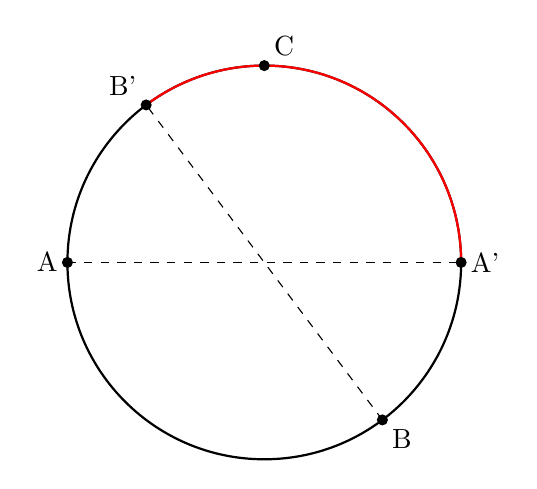
\begin{tikzpicture}
	\draw[thick] (0,0) circle(2.5cm);
	\draw[thick][red]
	(2.5,0) arc[start angle=0, end angle=127, radius=2.5cm];

	\fill (-2.5,0) circle (2pt) node[left] {A};
	\fill (1.5,-2) circle (2pt) node[below right] {B};
	\fill (0,2.5) circle (2pt) node[above right] {C};
	\fill (2.5,0) circle (2pt) node[right] {A'};
	\fill (-1.5,2) circle (2pt) node[above left] {B'};
	\draw[dashed] (-2.5,0) -- (2.5,0);
	\draw[dashed] (1.5,-2) -- (-1.5,2);

\end{tikzpicture}

Mając ustalony punkt \(A\) widzimy, że długość łuku \(AB\) jest
zmienną o rozkładzie jednostajnym na przedziale \([0, \pi r]\).

Dla dowolnego wyboru \(B\) prawdopodobieństwo, że \(C\) będzie dobre,
wynosi
\(\frac{\overset{\huge\frown}{A'B'}}{2\pi r}\)
\(= \frac{\overset{\huge\frown}{AB}}{2\pi r}\)

Średnia długość łuku to \(\frac{\pi r}2\), więc \(Pr = \frac 1 4\).

To widać, ale można ciut formalniej
\[
	\int_0^{\pi r} \frac{\frac{t}{\pi r}}{2\pi r}~dt
	= \frac{1}{2\pi^2r^2} \int_0^{\pi r} t~dt
	= \frac{1}{2\pi^2r^2} \cdot \frac {\pi^2r^2}2
	= \frac{1}{4}
\]

Bardzo drobnymi zmianami można zmienić to rozumowanie na bardzo podobne
do rozwiązania zadania 7., co pozostawiam jako ćwiczenie dla czytelnika.

\subsection*{Odpowiedź}
\[
	\boxed{\frac 1 4}
\]

\section{Zadanie 7}
\autor{Hubert Jastrzębski}
Łamiemy kij w dwóch niezależnie i jednostajnie wybranych punktach. Jakie
jest prawdopodobieństwo tego, że z otrzymanych kawałków można zbudować trójkąt?


\subsection*{Rozwiązanie}
Niech kij ma długość \(1\) i zostanie złamany w punktach \(X_1\) i \(X_2\), gdzie \(X_1, X_2 \sim \text{Unif}(0, 1)\).

Funkcje gęstości zmiennych losowych \(X_1\) i \(X_2\) są następujące:

\[
	f_1(x_1) = \frac{1}{1 - 0} = 1 \quad \text{dla } x_1 \in [0, 1] \quad \land \quad f_2(x_2) = \frac{1}{1 - 0} = 1 \quad \text{dla } x_2 \in [0, 1]
\]

Zmienne losowe są niezależne, więc ich funkcja gęstości wspólnej jest iloczynem funkcji gęstości poszczególnych zmiennych:
\[
	f(x_1, x_2) = f_1(x_1) \cdot f_2(x_2) = 1 \cdot 1 = 1 \quad \text{dla } x_1, x_2 \in [0, 1]
\]

Policzmy zdarzenie odwrotne, czyli prawdopodobieństwo, że z kawałków nie można zbudować trójkąta.
Oznacza to, że jeden z kawałków jest dłuższy niż \(0.5\).

Mamy trzy przypadki:

\medbreak
\textbf{1. Pierwszy kawałek jest długi:}

Przez pierwszy kawałek mam na myśli kawałek najbardziej po lewej stronie, który ma długość \(min(X_1, X_2)\).
Aby był długi (\(\geq 0.5\)), musi zachodzić \(X_1 \geq 0.5 \land X_2 \geq 0.5\).

Prawdopodobieństwo na to wynosi:
\[
	P(X_1 \geq 0.5 \land X_2 \geq 0.5) = P(X_1 \geq 0.5) \cdot P(X_2 \geq 0.5)
	= \int_{0.5}^{1} f(x_1) \, dx_1 \cdot \int_{0.5}^{1} f(x_2) \, dx_2 = \frac{1}{2} \cdot \frac{1}{2} = \frac{1}{4}
\]

\medbreak
\textbf{2. Trzeci kawałek jest długi:}

Analogicznie \(P(X_1 \leq 0.5 \land X_2 \leq 0.5) = \frac{1}{4}\)

\medbreak
\textbf{3. Drugi kawałek jest długi:}
\[
	P(|X_1 - X_2| \geq 0.5) = P(X_1 - X_2 \geq 0.5) + P(X_2 - X_1 \geq 0.5)
\]
\[
	= \int \int_{\{x_1 \geq x_2 + 0.5\}} f(x_1, x_2) \, dx_1 \, dx_2 + \int \int_{\{x_2 \geq x_1 + 0.5\}} f(x_1, x_2) \, dx_1 \, dx_2
\]

Rozważmy \(\int \int_{\{x_1 \geq x_2 + 0.5\}} f(x_1, x_2) \, dx_1 \, dx_2\):

Pamiętajmy, że \(x_1, x_2 \in [0, 1]\), więc \(x_2 + 0.5 \leq 1 \implies x_2 \leq 0.5\).

Natomiast dla ustalonego \(x_2\), \(x_1\) może przyjmować wartości od \(x_2 + 0.5\) do \(1\). Tak więc:

\[
	\int \int_{\{x_1 \geq x_2 + 0.5\}} f(x_1, x_2) \, dx_1 \, dx_2 = \int_{0}^{0.5} \int_{x_2 + 0.5}^{1} f(x_1, x_2) \, dx_1 \, dx_2
\]
\[
	= \int_{0}^{0.5} \int_{x_2 + 0.5}^{1} 1 \, dx_1 \, dx_2 = \int_{0}^{0.5} (1 - (x_2 + 0.5)) \, dx_2 = \int_{0}^{0.5} (0.5 - x_2) \, dx_2
\]
\[
	= \left[0.5x_2 - \frac{x_2^2}{2}\right]_{0}^{0.5} = \left(0.5 \cdot 0.5 - \frac{(0.5)^2}{2}\right) - (0) = \frac{1}{4} - \frac{1}{8} = \frac{1}{8}
\]

Analogicznie \(\int \int_{\{x_2 \geq x_1 + 0.5\}} f(x_1, x_2) \, dx_1 \, dx_2 = \frac{1}{8}\).

Tak więc \(P(|X_1 - X_2| \geq 0.5) = \frac{1}{8} + \frac{1}{8} = \frac{1}{4}\).

\medbreak
Sumując wszystkie przypadki mamy:
\[
	P(\text{jeden kawałek jest długi}) = \frac{1}{4} + \frac{1}{4} + \frac{1}{4} = \frac{3}{4}
\]
\[
	P(\text{żaden kawałek nie jest długi}) = 1 - \frac{3}{4} = \frac{1}{4}
\]

\subsection*{Odpowiedź}
\[
	\boxed{\frac{1}{4}}
\]

\section{Zadanie 8 (Oskar Prusik)}
Łamiemy kij długości \(1\) w jednostajnie losowo wybranym punkcie.
Niech \(X\) oznacza punkt złamania.


(i) Jaka jest oczekiwana długość krótszej części?  

(ii) Jaki jest oczekiwany stosunek długości części krótszej do części dłuższej?  

(iii) Jaki jest oczekiwany stosunek długości części dłuższej do części krótszej?


\subsection*{Rozwiązanie}
 Ponieważ wybór jest jednostajny na odcinku \([0,1]\), zmienna losowa \(X\) ma rozkład jednostajny na tym przedziale. Gęstość prawdopodobieństwa dana jest wzorem:

\[
f_X(x) = 
\begin{cases}
	1 & \text{dla } x \in [0,1] \\
	0 & \text{w pozostałych przypadkach}
\end{cases}
\]

Wprowadzamy oznaczenia:
\[
L = \min(X, 1-X), \quad D = \max(X, 1-X)
\]
gdzie \(L\) to długość krótszej części, a \(D\) to długość dłuższej części.

\subsection*{(i)}
\[
\mathbb{E}[L] = \int_{0}^{1} \min(x, 1-x) \cdot f_X(x) \, dx = \int_{0}^{1} \min(x, 1-x) \, dx
\]
Punkt \(x = 0.5\) jest punktem podziału:
\[
\mathbb{E}[L] = \int_{0}^{0.5} x \, dx + \int_{0.5}^{1} (1-x) \, dx
\]
Obliczamy:
\[
\int_{0}^{0.5} x \, dx = \left[ \frac{x^2}{2} \right]_{0}^{0.5} = \frac{0.25}{2} = 0.125
\]
\[
\int_{0.5}^{1} (1-x) \, dx = \left[ x - \frac{x^2}{2} \right]_{0.5}^{1} = (1-0.5) - (0.5 - 0.125) = 0.5 - 0.375 = 0.125
\]
\[
\mathbb{E}[L] = 0.125 + 0.125 = 0.25 = \frac14
\]

\subsection*{(ii)}
\[
R_1 = \frac{L}{D} = \frac{\min(x, 1-x)}{\max(x, 1-x)}
\]
\[
\mathbb{E}[R_1] = \int_{0}^{1} \frac{\min(x, 1-x)}{\max(x, 1-x)} \cdot f_X(x) \, dx = \int_{0}^{1} \frac{\min(x, 1-x)}{\max(x, 1-x)} \, dx
\]
Całkujemy po dwóch przedziałach:
\[
\mathbb{E}[R_1] = \int_{0}^{0.5} \frac{x}{1-x} \, dx + \int_{0.5}^{1} \frac{1-x}{x} \, dx
\]

Pierwsza całka:
\[
\int_{0}^{0.5} \frac{x}{1-x} \, dx = \int_{0}^{0.5} \left( \frac{1}{1-x} - 1 \right) dx
\]
\[
= \left[ -\ln(1-x) - x \right]_{0}^{0.5} = \left( -\ln 0.5 - 0.5 \right) - \left( -\ln 1 - 0 \right) = \ln 2 - 0.5
\]

Druga całka:
\[
\int_{0.5}^{1} \frac{1-x}{x} \, dx = \int_{0.5}^{1} \left( \frac{1}{x} - 1 \right) dx
\]
\[
= \left[ \ln x - x \right]_{0.5}^{1} = (\ln 1 - 1) - (\ln 0.5 - 0.5) = (-1) - (-\ln 2 - 0.5) = \ln 2 - 0.5
\]

Sumując:
\[
\mathbb{E}[R_1] = (\ln 2 - 0.5) + (\ln 2 - 0.5) = 2\ln 2 - 1
\]

\subsection*{(iii)}
\[
R_2 = \frac{D}{L} = \frac{\max(x, 1-x)}{\min(x, 1-x)}
\]
\[
\mathbb{E}[R_2] = \int_{0}^{1} \frac{\max(x, 1-x)}{\min(x, 1-x)} \cdot f_X(x) \, dx = \int_{0}^{1} \frac{\max(x, 1-x)}{\min(x, 1-x)} \, dx
\]
\[
\mathbb{E}[R_2] = \int_{0}^{0.5} \frac{1-x}{x} \, dx + \int_{0.5}^{1} \frac{x}{1-x} \, dx
\]

\noindent\textbf{Obliczenie pierwszej całki:}
\[
\int_{0}^{0.5} \frac{1-x}{x} \, dx = \int_{0}^{0.5} \left( \frac{1}{x} - 1 \right) dx
\]
Całka \(\int_{0}^{0.5} \frac{1}{x} \, dx\) jest rozbieżna, co pokazujemy przez granicę:
\[
\lim_{\varepsilon \to 0^+} \int_{\varepsilon}^{0.5} \frac{1}{x} \, dx = \lim_{\varepsilon \to 0^+} \left[ \ln x \right]_{\varepsilon}^{0.5} = \ln 0.5 - \lim_{\varepsilon \to 0^+} \ln \varepsilon = +\infty
\]
Nawet po odjęciu skończonej całki \(\int_{0}^{0.5} 1 \, dx = 0.5\), pierwsza całka dąży do nieskończoności.

\noindent\textbf{Obliczenie drugiej całki:}
\[
\int_{0.5}^{1} \frac{x}{1-x} \, dx = \int_{0.5}^{1} \left( \frac{1}{1-x} - 1 \right) dx
\]
\[
= \left[ -\ln(1-x) - x \right]_{0.5}^{1}
\]
W \(x=1\): \(-\ln(0) - 1\) - tutaj \(\ln 0 = -\infty\), ale liczymy granicę:
\[
\lim_{t \to 1^-} \left[ -\ln(1-t) - t \right]_{0.5}^{t} = \lim_{t \to 1^-} \left[ (-\ln(1-t) - t) - (-\ln 0.5 - 0.5) \right]
\]
\[
= \lim_{t \to 1^-} \left[ -\ln(1-t) - t + \ln 0.5 + 0.5 \right]
\]
Człon \(-\ln(1-t) \to +\infty\), więc całka od \(0.5\) do \(1\) też jest rozbieżna!

Zatem obie całki w \(\mathbb{E}[R_2]\) są rozbieżne do \(+\infty\), co potwierdza:
\[
\mathbb{E}[R_2] = \infty
\]

\subsection*{Odpowiedź}
\[
\boxed{\text{(i) } \frac14} \quad \boxed{\text{(ii) } 2\ln 2 - 1} \quad \boxed{\text{(iii) } \infty}
\]

\section{Zadanie 9}
Niech $X$ oraz $Y$ będą zmiennymi losowymi z rozkłądu jednostajnego na przedziale $[0, 1]$.
Jakie jest prawdopodobieństwo tego, że najbliższa liczba całkowita do ilorazu $X/Y$ jest parzysta?
Wynik przedstaw w formie $a + b\pi$.

\subsection*{Rozwiązanie}
$$f(x, y) = \begin{cases}
                f_{1}(x, y), & x \leqslant y,\\
                f_{2}(x, y), & \text{wpp}.
            \end{cases}
$$
$$
f_{1}(x, y) = \begin{cases}
                  1, & y \in [2*x, 1],\\
                  0, & \text{wpp}.
\end{cases}
$$
$$
f_{2}(x, y) = \begin{cases}
                  1, & y \in \cup_{i=0}^{\infty}[\frac{2x}{4i+5}, \frac{2x}{4i+3}],\\
                  0, & \text{wpp}.
\end{cases}
$$

$$ P(\text{round}(\frac{X}{Y}) - \text{parzyste}) = \int_{0}^{1}\int_{0}^{1}f(x, y)dydx = \int_{0}^{1}\int_{x}^{1}f_1(x, y)dydx + \int_{0}^{1}\int_{0}^{x}f_2(x, y)dydx = $$
$$ = \int_{0}^{\frac{1}{2}}\int_{2x}^{1}dydx + \int_{0}^{1}\sum_{i=0}^{\infty}\int_{\frac{2x}{2i+5}}^{\frac{2x}{2i+3}}dydx = \int_{0}^{\frac{1}{2}}(1 - 2x)dx + \int_{0}^{1}\sum_{i=0}^{\infty}(\frac{2x}{2i+3} - \frac{2x}{2i+5})dx = $$
$$ = \frac{1}{2} - \frac{1}{4} + \int_{0}^{1}2x\sum_{i=1}^{\infty}\frac{(-1)^{(i+1)}}{2i + 1}dx = \frac{1}{4} + \int_{0}^{1}2x(1 - \frac{\pi}{4})dx = \frac{1}{4} + 1 - \frac{1}{4}\pi = \frac{5}{4} - \frac{1}{4}\pi$$

\subsection*{Odpowiedź}
\[
\boxed{\frac{5}{4} - \frac{1}{4}\pi}
\]

\section{Zadanie 10}
Losujemy \(n\) przedziałów \(I_1, \dots, I_n\) w następujący sposób: konstruując \(i\)-ty przedział losujemy niezależnie i jednostajnie jego oba końce z przedziału \([0, 1]\). Jakie jest prawdopodobieństwo tego, że istnieje punkt \(p\) należący do wszystkich wylosowanych przedziałów?


\subsection*{Rozwiązanie}
Sprowadzamy zadanie do dyskretnego problemu. Wylosujmy wszystkie końce \(X_1,\dots,X_n\) oraz \(Y_1,\dots,Y_n\) i posortujmy otrzymując \(Z_1,\dots,Z_{2n}\). Aby istniał punkt \(p\), należący do wszystkich przedziałów, musi się on znajdować w przedziale \((Z_n,Z_{n+1})\) i dla każdego \(I_k\) jeden z jego krańców musi być w \((Z_1,\dots,Z_n)\), a drugi w \((Z_{n+1},\dots,Z_{2n})\). Prawdopodobieństwo takiego zdarzenia wynosi
\[
	P = \frac{2^n (n!)^2}{(2n)!}
\]
Ze względu na \(2^n\) możliwości wyboru części \(Z\)-tów dla krańców każdego przedziału, a \(\frac{(n!)^2}{(2n)!}\) na spermutowanie.
\subsection*{Odpowiedź}
\[
	\boxed{{P = \frac{2^n (n!)^2}{(2n)!}}}
\]

\section{Zadanie 11}
(igła Buffona)
Płaszczyznę przecięto zbiorem poziomych linii. Odstęp między dwoma
sąsiednimi liniamy wynosi \(d\). Rzucamy igłą długości \(l\) na tę
płaszczyznę. Wyznacz prawdopodobieństwo przecięcia linii.
\subsection*{Rozwiązanie}
Rozważymy dwa przypadki
\subsubsection*{Igła krótsza (lub równa) od dystansu między liniami}
Mamy \(l \leq d\). Jeśli igła po rzuceniu utworzy z liniami 
jakiś kąt ostry \(\alpha\), to przetnie się z taką linią, której
odległość od środka igły była co najwyżej
\(\frac{l}{2}\cdot\sin \alpha\).
\begin{center}
  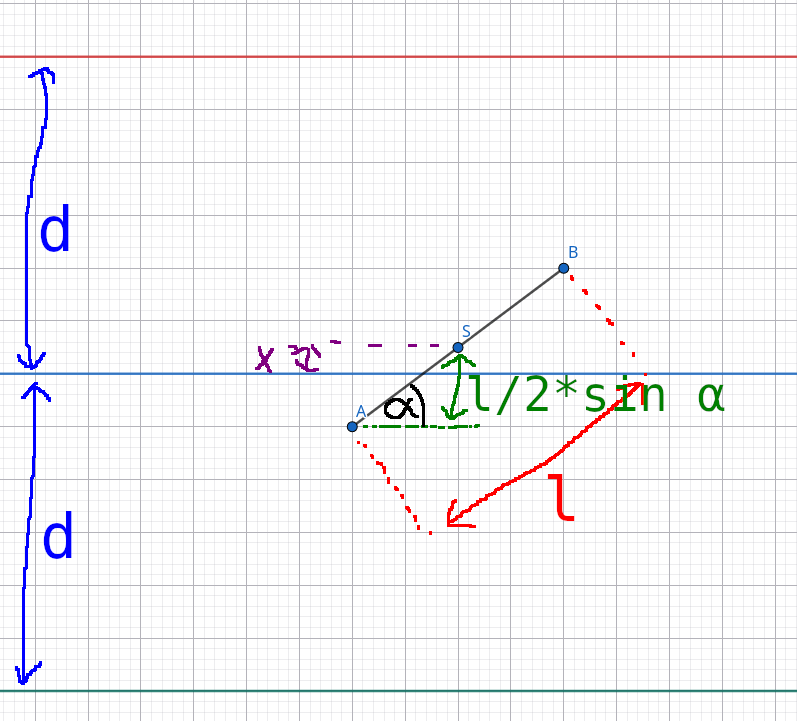
\includegraphics[width=0.7\textwidth]{tasks/11-1.png}
\end{center}

Zdarzenie jest cykliczne, więc możemy założyć że
\(\alpha \in \big[0, \frac{\pi}{2}\big]\).
\(\alpha\) ma rozkład jednostajny.

Odległość \(X\) środka igły od najbliższej linii przyjmuje wartości z przedziału
\(\big[0, \frac{d}{2}\big]\). Ma rozkład jednostajny.

\[
    P(\text{sukces})
    = P\left(\frac{l}{2}\sin \alpha \geq X\right)
    = \int_0^{\frac{\pi}2} \frac{2}{\pi} 
    \cdot \left(\frac{l}{2}\sin \alpha \right) \cdot 
    \frac{2}{d}~d\alpha
\]
Gdzie rozbiliśmy zdarzenie na podzdarzenia: \(X\) większy od już
ustalonego \(\alpha\)
\begin{itemize}
    \item \(\frac{2}{\pi}\) --- gęstość rozkładu \(\alpha\) (jednostajna)
    \item \(\frac{l}{2}\sin \alpha\) --- "ilość" takich \(X\)-ów, które
    spełniają nierówność
    \item \(\frac{2}{d}\) --- gęstość zmiennej \(X\) (jednostajna)
\end{itemize}
W prezentacji https://probabil.tcs.uj.edu.pl/docs/igla.pdf
jest przedstawione to samo za pomocą całki podwójnej, tutaj został
pominięty ten krok.

\[
    P(\text{sukces})
    = \frac{2l}{\pi d} \int_0^{\frac{\pi}2} \sin \alpha
    = \frac{2l}{\pi d}~(-\cos\alpha) \Big|_{0}^{\frac{\pi}{2}}
    = \frac{2l}{\pi d} \cdot 1
    = \frac{2l}{\pi d}
\]

\subsubsection*{Igła dłuższa od dystansu między liniami}
Mamy \(l > d\). Po ustaleniu jakiejś \(\alpha\), mieliśmy
\(
P(X \leq \frac{l}{2}\sin\alpha) = 
\frac{l}{2}\sin \alpha \cdot \frac{2}{d}
\).

Teraz nie jest to już prawdą. Może się zdarzyć, że dla jakiejś
\(\alpha\), nie jest możliwe wylosowanie \(X\) który nie spełni nierówności.

Na przykład, dla \(\alpha = \frac{\pi}{2}\).
Igła jest pionowo i jest dłuższa niż dystans między liniami,
więc na pewno którąś przetnie. Według naszego naiwnego wzorku
ma na to prawdopobieństwo \(\frac{l}{d} > 1\).

Dopóki \(\frac{l}{d}\sin \alpha\) nie przekracza 1 wszystko działa. Można
więc policzyć:

\[
    P(\text{sukces})
    = P\left(\frac{l}{2}\sin \alpha \geq X\right)
    = \int_0^{\frac{\pi}2} \frac{2}{\pi} 
    \cdot
    \max\left(1,~\frac{l}{2}\sin \alpha \frac{2}{d}
    \right)
    ~d\alpha
\]

Mamy \(\frac{l}{d}\sin\alpha > 1\) wtw. \(\alpha > \arcsin \frac{d}{l}\).
Można więc łatwo rozbić na sumę dwóch całek

\[
    \frac{2}{\pi} \int_0^{\frac{\pi}2} 
    \max\left(1,~\frac{l}{d}\sin \alpha \right)
    ~d\alpha
    = \frac{2}{\pi} \left(
    \int_0^{\arcsin\frac{d}{l}} \frac{l}{d}\sin \alpha
    +
    \int_{\arcsin\frac{d}{l}}^{\frac{\pi}{2}} d\alpha
    \right)
\]
\[
    = \frac{2}{\pi} \left(
    \frac{l}{d}~(-\cos\alpha) \Big|_{0}^{\arcsin\frac{d}{l}}
    + \left(\frac{\pi}{2} - \arcsin\frac{d}{l} \right)
    \right)
\]
\[
    = \frac{2}{\pi} \left(
    \frac{l}{d}\left(1 - \cos\left(\arcsin\left(\frac{d}{l}
    \right)\right)\right)
    + \left(\frac{\pi}{2} - \arcsin\frac{d}{l} \right)
    \right)
\]
\[
    \frac{2l}{\pi d} \left(
    1 - \sqrt{1 - \left(\frac{d}{l}\right)^2}\right)
    + \frac{2}{\pi}\arccos\frac{d}{l}
\]

\subsection*{Odpowiedź}
\[
\boxed{
\frac{2l}{\pi d}\text{, gdy } l \leq d
}
\]
\[
\boxed{
    \frac{2l}{\pi d} \left(
    1 - \sqrt{1 - \left(\frac{d}{l}\right)^2}\right)
    + \frac{2}{\pi}\arccos\frac{d}{l}
    \text{, gdy } l > d
}
\]

\section{Zadanie 12 (Aleksander Wieczorek)}
(krzyżyk Buffona) Na płaszczyznę przeciętą równoległymi liniami o odstępie
1 rzucono dwie jednostkowe igły sklejone prostopadle środkami. Niech Z będzie liczbą
przecięć tak utworzonego krzyżyka z liniami. Policz E(Z) i Var(Z).

\subsection*{Rozwiązanie}
Rozbijmy Z na indykatory:
$$Z=X_1+X_2$$
Gdzie $X_1=1$ gdy 1. igła przecina deskę i 0 w p.p. Analogicznie dla $X_2$\\
Teraz już łatwo policzyć E(Z), bo:
$$E(Z) = E(X_1)+E(X_2)=P(X_1=1)+P(X_1=1) = 2\cdot \frac{2}{\pi} = \frac{4}{\pi}$$\footnote{Dowód tego, że P(igła przecina deskę)=$\frac{2}{\pi}$ jest poprzednim zadaniem, więc go pominę}
Wariancję też liczymy wzorem:
$$Var(Z) = Var(X_1)+Var(X_2)+2Cov(X_1,X_2)$$
Z własności indykatorów mamy:
$$Var(X_1)=Var(X_2)=p(1-p)=\frac{2}{\pi}\left(1-\frac{2}{\pi}\right)=\frac{2\pi-4}{\pi^2}$$
$$Cov(X_1,X_2)=E(X_1X_2)-E(X_1)E(X_2)=P(X_1=1 \cap X_2=1)-\frac{4}{\pi^2}$$
Teraz niestety musimy rozpatrzeć przypadek gdy obie igły przecinaj deskę jednocześnie. Do tego przyda się rysunek:
\begin{center}

    \begin{tikzpicture}[scale=1]

        \draw[thick] (-3,-1) -- (-3,7);
        \draw[thick] (7,-1) -- (7,7);

        \draw[thick] (7,6) -- (3,3) -- (7,3);
        \draw[thick] (3,3) -- (7,0);
        \tkzDefPoints{3/3/O,7/6/A,7/3/B,7/0/C};
        \tkzMarkAngle[size = 2.5, arc=ll](B,O,A);
        \tkzMarkAngle[size = 2.5, arc=ll](C,O,B);
        \tkzLabelAngle[dist=1.5](B,O,A){\(\theta\)};
        \tkzLabelAngle[dist=1.5](C,O,B){\(90-\theta\)};
        \tkzDefPoint(6,3){X};
        \tkzLabelPoint[above, black](X){\(x\)};

        \tkzDefPoint(5,4.5){Y};
        \tkzLabelPoint[above, black](Y){\(y\)};

        \tkzDefPoint(5,1.5){Z};
        \tkzLabelPoint[below, black](Z){\(z\)};
        
        \draw[red,thick,dashed, <->] (-3,6.5) -- (7, 6.5);

        \tkzDefPoint(2,6.5){D};
        \tkzLabelPoint[above, black](D){\(1\)};
    \end{tikzpicture}
\end{center}
Igły przetną deskę wtw. $y\le\frac{1}{2} \wedge z\le\frac{1}{2}$\\
Mamy również: $\cos(\theta)=\frac{x}{y}$ oraz $sin(\theta)=\cos(90-\theta)=\frac{x}{z}$
Po prostym przekształceniu i podstawieniu mamy:
$$x\le\frac{\cos(\theta)}{2} \wedge x\le\frac{sin(\theta)}{2}$$
Wystarczy policzyć prawdopodobieństwo, że zmienna X (odległość od deski) jest nie większa niż $\frac{min(sin(\theta),\cos(\theta))}{2}$
Zauważmy, że to minimum to $sin(\theta)$ dla $0\le \theta\le \frac{\pi}{4}$ oraz $\cos(\theta)$ dla $\frac{\pi}{4}\le \theta\le \frac{\pi}{2}$
Teraz zapiszmy gęstości X,$\theta$ i ich splotu.\\
$$f_X(x)=2\text{ dla $x\in (0,\frac{1}{2})$ }\footnote{Dla uproszczenia zapisu poza podanym przedziałem gęstość to 0. Tak samo dla innych gęstości}$$
$$f_\theta(x)=\frac{2}{\pi}\text{ dla $\theta\in (0,\frac{\pi}{2})$ }$$
Ponieważ X i $\theta$ niezależne to gęstość ich splot to iloczyn ich gęstości
$$f_{X\theta}(x)=\frac{4}{\pi}\text{ dla $\theta\in (0,\frac{\pi}{2})$ $x\in (0,\frac{1}{2})$ }$$
Teraz niestety trzeba policzyć całkę:
$$E(X_1X_2)=P\left(X\le \frac{min(sin(\theta),\cos(\theta))}{2}\right)=\int_0^\frac{\pi}{4}\int_0^{\frac{sin(\theta)}{2}} f_{X\theta}(x) dxd\theta + \int_\frac{\pi}{4}^\frac{\pi}{2}\int_0^{\frac{\cos(\theta)}{2}} f_{X\theta}(x) dxd\theta=$$
$$\frac{4}{\pi}\left(\int_0^\frac{\pi}{4}\int_0^{\frac{sin(\theta)}{2}}1 dxd\theta + \int_\frac{\pi}{4}^\frac{\pi}{2}\int_0^{\frac{\cos(\theta)}{2}} 1 dxd\theta \right)=$$
$$\frac{2}{\pi}\left(\int_0^\frac{\pi}{4}sin(\theta)d\theta + \int_\frac{\pi}{4}^\frac{\pi}{2} \cos(\theta)d\theta \right)=\frac{2}{\pi}(\left[-\cos(\theta)\right]_0^{\pi/4} + \left[sin(\theta)\right]_{\pi/4}^{\pi/2})=$$
$$\frac{2}{\pi}\left(\frac{-\sqrt{2}}{2}+1 +1 - \frac{-\sqrt{2}}{2}\right)=\frac{4-2\sqrt{2}}{\pi}$$
Teraz nareszcie możemy wstawić wszystko z powrotem do wzoru:
$$Cov(X_1,X_2)=\frac{4-2\sqrt{2}}{\pi}-\frac{4}{\pi^2}=\frac{4\pi-2\pi\sqrt{2}-4}{\pi^2}$$
$$Var(Z)=2\cdot \frac{2\pi-4}{\pi^2} + 2 \cdot\frac{4\pi-2\pi\sqrt{2}-4}{\pi^2}=\frac{12\pi-4\pi\sqrt{2}-16}{\pi^2}$$
\subsection*{Odpowiedź}
\[
\boxed{E(Z) = \frac{4}{\pi} \quad
Var(Z)=\frac{12\pi-4\pi\sqrt{2}-16}{\pi^2}
}
\]
\section{Zadanie 13}

Wybierz punkt $X$ w sposób losowy i jednostajny z okręgu $O$ o średnicy 1 i o środku w punkcie (0, 10). Rozważ średnicę $O$ o końcu w punkcie $X$. Jaka jest oczekiwana długość projekcji tej średnicy na oś $OX$.

\subsection*{Rozwiązanie}

Fakt 1:

Położenie środka nie ma znaczenia, ponieważ długość projekcji, zależy tylko do średnicy i jest one relatywne względem środka.

Fakt 2

Jeśli $X$ jest na dolnej połówce, to można go zmainić, na symetryczny $X$ na górnej połówce, co pokazuję, że wystarczy obliczyć dla X w górnej połówce razy 2.

Fakt 3:

Z pozostałych ćwiartek, wystarczy wziąść lewą ćwiartkę i ze względu na symetryzm da nam to dobry wynik.


Teraz obliczemy Dystrybuante zmiennej $X$. dla danego $x$. PRzypomniejmy, że $F(x) = P(X < x)$. W sumie bardziej będzie nas intersowało obliczyć dopełnienie $F(X)$ (bo jest łatwiej policzyć, a 1 zniknie i tak przy pochodnej). 

Żeby policzyć $1 - F(x)$ patrzymy trygonometrycznie, na kąt $\alpha$, między średnicą $O$, a jej projekcją. 

\[
    cos(\alpha) = \frac{x}{\frac{1}{2}} = 2 \cdot x
\]
\[
    \alpha = arccos(2x)
\]
Możemy zauważyć, że prawdopodobieńwo, że $X$ jest większe niż $x$ jest równe ułamkowii $\frac{\alpha}{\frac{2}{\pi}}$

\[
    1 - F(X) =  \frac{\alpha}{\frac{\pi}{2}} = \frac{\alpha \cdot 2}{\pi} = \frac{arccos(2x) \cdot 2}{\pi}
\]
\[
    F(X) = 1 - \frac{arccos(2x) \cdot 2}{\pi}
\]
\[
    f(X) = F(X)' = \frac{4}{\pi} \cdot \frac{1}{\sqrt{1 - 4 x^2}}
\]
\[
    E[X] = \int_{0}^{\frac{1}{2}} x \cdot f(x)\,dx = \frac{4}{\pi} \int_{0}^{\frac{1}{2}} x \cdot \frac{1}{\sqrt{1 - 4x^2}} = [t = 1 - 4x^2, dt = -8x\,dt] = 
\]
\[
    E[X] = \frac{4}{\pi} \cdot \int_{1}^{0} \frac{1}{\sqrt{t}} \cdot \frac{-1}{8}\,dt = \frac{1}{2 \pi} \cdot \int_{0}^{1} \frac{1}{\sqrt{t}}\,dt = \frac{1}{2 \pi} \cdot (2 \cdot 1 - 2 \cdot 0) = \frac{1}{2 \pi} \cdot 2 = \frac{1}{\pi}
\]

Pamiętajmy, jeszcze, że musimy $E(x)$ pomnożyć razy $2$, więc:
\[
    E(X) = 2 \cdot \frac{1}{\pi} = \frac{2}{\pi}
\]


\section{Zadanie 14}
Z kwadratu jednostkowego \([0, 1] \times [0, 1]\) losujemy punkt w sposób jednostajny.
Później niezależnie wybieramy kąt w sposób jednostajny na \([0, 2\pi]\).
Z jakim prawdopodobieństwem odcinek jednostkowy rozpoczynający się w wylosowanym punkcie
zmierzający w kierunku wylosowanego kąta wychodzi poza rozważany kwadrat?

\subsection*{Rozwiązanie}

\begin{center}
	\begin{tikzpicture}[scale=3.5]
		% Kwadrat [0,1]x[0,1]
		\draw[thick] (0,0) rectangle (1,1);

		% Punkt Q
		\filldraw[red] (0.7,0.4) circle (0.02);
		\node[below left] at (0.7,0.4) {$(x, y)$};

		% Długość odcinka
		\def\L{1}

		% Kąt w stopniach
		\def\kat{160}

		% Punkt R (koniec odcinka)
		\coordinate (R) at ($(0.7,0.4) + (160:\L)$);

		% Odcinek Q -> R
		\draw[blue, thick] (0.7,0.4) -- (R);

		% Zaznaczenie końcowego punktu R
		\filldraw[green] (R) circle (0.02);
		\node[above left] at (R) {$(x+\cos\theta, \; y+\sin\theta)$};

		% Łuk kąta theta (promień 0.25)
		\draw[->, thick, orange]
		(0.7,0.4) ++(0:0.25) arc (0:\kat:0.25) {};

		% Podpis kąta
		\node at ($(0.7,0.4)+(0.02,0.12)$) {$\theta$};
	\end{tikzpicture}
\end{center}

Niech punkt startu to \((x,y)\) i kąt \(\theta\). Koniec odcinka jednostkowego ma współrzędne:
\[
	(x+\cos\theta, \; y+\sin\theta).
\]

Odcinek pozostaje w kwadracie wtedy i tylko wtedy gdy punkt końca odcinka jednostkowego jest w kwadracie, czyli:
\[
	0 \le x + \cos\theta \le 1 \quad \text{oraz} \quad 0 \le y + \sin\theta \le 1.
\]

Dla ustalonego \(\theta\), dopuszczalne wartości \(x\) (z pierwszej nierówności) to:
\[
	x \in [0,1] \cap [-\cos\theta, 1-\cos\theta],
\]
długość tego przedzialu wynosi \(1 - |\cos\theta|\). Analogicznie dla \(y\): \(1 - |\sin\theta|\).

Zatem prawdopodobieństwo, że odcinek pozostaje w kwadracie dla ustalonego \(\theta\), to:
\[
	(1 - |\cos\theta|)(1 - |\sin\theta|).
\]
Teraz wystarczy uśrednić ten wynik po wylosowanym kącie \\
Uśredniając po \(\theta\), otrzymujemy:
\[
	P_{\text{wewnątrz}} = \frac{1}{2\pi} \int_0^{2\pi} (1 - |\cos\theta|)(1 - |\sin\theta|) \, d\theta.
\]

Rozwijamy iloczyn pod całką:
\[
	(1 - |\cos\theta|)(1 - |\sin\theta|) = 1 - |\cos\theta| - |\sin\theta| + |\cos\theta||\sin\theta|.
\]

Zatem:
\[
	P_{\text{wewnątrz}} = 1 - \frac{1}{2\pi} \int_0^{2\pi} (|\cos\theta| + |\sin\theta|) \, d\theta + \frac{1}{2\pi} \int_0^{2\pi} |\cos\theta||\sin\theta| \, d\theta.
\]

Obliczamy całki:
\[
	\int_0^{2\pi} |\cos\theta| \, d\theta = 4, \quad \int_0^{2\pi} |\sin\theta| \, d\theta = 4, \quad \int_0^{2\pi} |\cos\theta||\sin\theta| \, d\theta = 2.
\]

Finalnie:
\[
	P_{\text{wewnątrz}} = 1 - \frac{4+4}{2\pi} + \frac{2}{2\pi} = 1 - \frac{6}{2\pi} = 1 - \frac{3}{\pi}.
\]

Zatem prawdopodobieństwo, że odcinek wychodzi poza kwadrat, wynosi:
\[
	P_{\text{wychodzi}} = \frac{3}{\pi}
\]


\subsection*{Odpowiedź}
\[
	\boxed{\frac{3}{\pi}}
\]

\section{Zadanie 15}
\autor{Filip Manijak}
Niech \(X, Y, Z\) będą niezależnymi zmiennymi losowymi o rozkładzie jednostajnym na przedziale \([0, 1]\). Niech \(U = XY\) i \(V = Z^2\).

\begin{enumerate}[label=(\roman*)]
	\item Wyznacz dystrybuantę, gęstość, wartość oczekiwaną i wariancję \(U\).
	\item Wyznacz dystrybuantę, gęstość, wartość oczekiwaną i wariancję \(V\).
	\item Oblicz \(P(U < V)\).
	\item Wyznacz \(E(X | U)\).
\end{enumerate}

\subsection*{Rozwiązanie}
\subsection{U}
Liczymy Dystrybuante:
\[F_U(a) =P(XY\leq a) = \int_0^1f_X(x)\int^{\frac{a}{x}}_0f_Y(y)dy dx = \int_0^af_X(x)*1+ \int_a^1f_X(x) F_Y(\frac{a}{x}) dx =\]
\[ =a+ \int^1_a \frac{a}{x} =a -a \ln a\]
Teraz z tego liczymy funkcję gęstości:
\[f_U(a) = F'_U(a) = (a-a \ln a)' = 1 - \ln a -1 = -\ln a\]
Liczymy też \(E[U]\):
\[E[U] = \int_0^1 f_U(x)xdx = -\int_0^1 x\ln x dx =-\left[ \frac{x^2}{2} \left( \ln x -\frac{1}{2} \right) \right]_0^1  = \frac{1}{4}\]
Zauważmy, że \(\lim_{x\xrightarrow{ }0}x^2 \ln x =0\) bo de l'Hospital. Całkę liczymy całkując przez części. Została wariancja:
\[Var[U] = E[U^2] - E[U]^2 = \int_0^1x^2(-\ln x) dx - \frac{1}{16} =\frac{1}{9} -  \frac{1}{16}\]
Tu też całkę liczymy całkując przez części.
\subsection{V}
Liczymy Dystrybuantę (dla \(a \in (0,1)\)):
\[F_V(a) = P(Z^2 \leq a) = P(-\sqrt{a} \leq Z \leq \sqrt{a}) = \int_0^{\sqrt{a}} 1 dz = \sqrt{a}\]
Teraz z tego liczymy funkcję gęstości:
\[f_V(a) = F'_V(a) = (\sqrt{a})' = \frac{1}{2\sqrt{a}}\]
Liczymy też \(E[V]\):
\[E[V] = \int_0^1 a f_V(a) da = \int_0^1 a \frac{1}{2\sqrt{a}} da = \frac{1}{2} \int_0^1 a^{\frac{1}{2}} da = \frac{1}{2} \left[ \frac{2}{3}a^{\frac{3}{2}} \right]_0^1 = \frac{1}{3}\]
Tutaj całkę liczymy prosto ze wzoru na funkcję potęgową (\(x^n\)). Została wariancja:
\[Var[V] = E[V^2] - E[V]^2 = \int_0^1 a^2 \frac{1}{2\sqrt{a}} da - \frac{1}{9} = \frac{1}{2} \int_0^1 a^{\frac{3}{2}} da - \frac{1}{9} = \frac{1}{5} - \frac{1}{9} = \frac{4}{45}\]
Tu również całkę liczymy jako funkcję potęgową.
\subsection{\(P(U<V)\)}
Zauważmy, że:
\[ P(U< V) = \int_0^1 f_V(x) F_U(x) dx = \int^1_0 \frac{1}{2\sqrt{x}}(x - x\ln x) dx = \frac{1}{2} \left( \int_0^1 \sqrt{x} dx - \int_0^1 \sqrt{x} \ln x dx \right)=\]
\[= \frac{1}{3} - \frac{1}{2}\left[\frac{2}{3}x\sqrt{x}\left(\ln x - \frac{2}{3}\right) \right]^1_0 = \frac{1}{3} - \frac{1}{2} \left( 0 - \frac{4}{9} \right) = \frac{1}{3} + \frac{2}{9} = \frac{5}{9}\]
\subsection{\(E[X | U]\)}
Chcemy obliczyć \(E[X | U](a) = \int_{-\infty}^{\infty} x f_{X|U=a}(x) dx\). W tym celu musimy wyznaczyć gęstość warunkową \(f_{X|U=a}(x)\).
Skorzystamy ze wzoru:
\[f_{X|U=a}(x) = \frac{f_{X,U}(x,a)}{f_U(a)}\]
Mianownik już znamy: \(f_U(a) = -\ln a\). Licznik (gęstość łączną) wyznaczymy, licząc pochodną  z dystrybuanty  \(F_{X,U}(x,a)\).

Dla \(a < x \le 1\):
\[F_{X,U}(x, a) = P(X \le x, XY \le a) = P(X \le a) + P(a < X \le x, Y \le \frac{a}{X}) =\]
\[= \int_0^a 1 dt + \int_a^x \frac{a}{t} dt = a + a(\ln x - \ln a)\]
Liczymy gęstość łączną:
\[f_{X,U}(x, a) = \frac{\partial^2 F_{X,U}}{\partial x \partial a} = \frac{\partial}{\partial a} \left( \frac{\partial}{\partial x} (a + a\ln x - a\ln a) \right) = \frac{\partial}{\partial a} \left( \frac{a}{x} \right) = \frac{1}{x}\]
Zatem gęstość warunkowa dla \(x \in [a, 1]\) wynosi:
\[f_{X|U=a}(x) = \frac{\frac{1}{x}}{-\ln a} = \frac{-1}{x \ln a}\]
Stąd wartość oczekiwana:
\[E[X | U=a] = \int_a^1 x \cdot f_{X|U=a}(x) dx = \int_a^1 x \left( \frac{-1}{x \ln a} \right) dx =\]
\[= \frac{-1}{\ln a} \int_a^1 1 dx = \frac{-1}{\ln a} [x]_a^1 = \frac{-(1-a)}{\ln a} = \frac{a-1}{\ln a}\]

\section{Zadanie 16}
\autor{Mateusz Wojaczek}
Niech \(X\) i \(Y\) mają łączną gęstość \(f(x, y) = cx(y - x)e^{-y}\) dla \(0 \le x \le y < \infty\).

\begin{enumerate}
	\item Wyznacz wartość \(c\).
	\item Udowodnij, że
	      \begin{align*}
		      f_{X|Y}(x | y) & = 6x(y - x)y^{-3} \quad \text{dla } 0 \le x \le y,           \\
		      f_{Y|X}(y | x) & = (y - x)e^{x - y} \quad \text{dla } 0 \le x \le y < \infty.
	      \end{align*}
	\item Wynioskuj, że \(\text{E}(X | Y) = \frac{1}{2}Y\) oraz \(\text{E}(Y | X) = X + 2\).
\end{enumerate}

\subsection*{Rozwiązanie}
\subsection*{(i) Wyznaczenie stałej \(c\)}

Aby \(f_{X,Y}(x,y)\) była gęstością, całka podwójna musi wynosić 1:
\[
	\int_0^\infty \int_0^y c x (y-x) e^{-y} \, dx \, dy = 1.
\]

Najpierw całkujemy względem \(x\):
\[
	\int_0^y x(y-x) dx = \int_0^y (xy - x^2) dx = \frac{1}{2}y^3 - \frac{1}{3}y^3 = \frac{1}{6}y^3.
\]

Zatem:
\[
	\int_0^\infty c \cdot \frac{1}{6} y^3 e^{-y} dy = 1 \implies \frac{c}{6} \int_0^\infty y^3 e^{-y} dy = 1.
\]

\(\int_0^\infty y^3 e^{-y} dy = 6\), więc:
\[
	\frac{c}{6} \cdot 6 = c = 1.
\]

\textbf{Odpowiedź:} \(c = 1\).

\subsection*{(ii) Wyznaczenie gęstości warunkowych}

\paragraph{Gęstość warunkowa \(X\) przy \(Y=y\)}:

\[
	f_{X|Y}(x|y) = \frac{f_{X,Y}(x,y)}{f_Y(y)}.
\]

Najpierw obliczamy \(f_Y(y)\):
\[
	f_Y(y) = \int_0^y f_{X,Y}(x,y) dx = \int_0^y 6 x (y-x) e^{-y} dx = 6 e^{-y} \cdot \frac{1}{6} y^3 = y^3 e^{-y}.
\]

Zatem:
\[
	f_{X|Y}(x|y) = \frac{6 x (y-x) e^{-y}}{y^3 e^{-y}} = \frac{6 x (y-x)}{y^3}, \quad 0 \le x \le y.
\]

\paragraph{Gęstość warunkowa \(Y\) przy \(X=x\)}:

\[
	f_{Y|X}(y|x) = \frac{f_{X,Y}(x,y)}{f_X(x)}.
\]

Najpierw obliczamy \(f_X(x)\):
\[
	f_X(x) = \int_x^\infty 6 x (y-x) e^{-y} dy = 6x \int_x^\infty (y-x) e^{-y} dy.
\]

Podstawiamy \(u = y-x \implies dy = du, y-x = u, y = u+x\):
\[
	\int_x^\infty (y-x) e^{-y} dy = \int_0^\infty u e^{-(u+x)} du = e^{-x} \int_0^\infty u e^{-u} du = e^{-x} \cdot 1! = e^{-x}.
\]

Zatem \(f_X(x) = 6 x e^{-x}\). Wobec tego:
\[
	f_{Y|X}(y|x) = \frac{6 x (y-x) e^{-y}}{6 x e^{-x}} = (y-x) e^{-(y-x)}, \quad y \ge x.
\]

\subsection*{(iii) Wartości oczekiwane warunkowe}

\paragraph{Dla \(E(X|Y)\)}:

\[
	E(X|Y=y) = \int_0^y x f_{X|Y}(x|y) dx = \int_0^y x \cdot \frac{6x(y-x)}{y^3} dx = \frac{6}{y^3} \int_0^y (x^2 y - x^3) dx.
\]

\[
	\int_0^y (x^2 y - x^3) dx = y \cdot \frac{y^3}{3} - \frac{y^4}{4} = \frac{y^4}{3} - \frac{y^4}{4} = \frac{y^4}{12}.
\]

\[
	E(X|Y=y) = \frac{6}{y^3} \cdot \frac{y^4}{12} = \frac{y}{2}.
\]

\paragraph{Dla \(E(Y|X)\)}:

\[
	E(Y|X=x) = \int_x^\infty y f_{Y|X}(y|x) dy = \int_x^\infty y (y-x) e^{-(y-x)} dy.
\]

Podstawiamy \(u = y-x \implies y = u+x, dy = du\):
\[
	E(Y|X=x) = \int_0^\infty (u+x) u e^{-u} du = \int_0^\infty u^2 e^{-u} du + x \int_0^\infty u e^{-u} du = 2 + x \cdot 1 = x + 2.
\]


\[
	E(X|Y) = \frac{1}{2}Y, \quad E(Y|X) = X+2.
\]

\subsection*{Odpowiedź}
\[
	\boxed{
		\begin{aligned}
			 & \textbf{Wartość } c\textbf{:}           &  & \mathbf{c = 1}                                                                       \\
			 & \textbf{Gęstości warunkowe:}            &  & f_{X|Y}(x | y) = \mathbf{6x(y - x)y^{-3}}, \quad \text{dla } 0 \le x \le y           \\
			 &                                         &  & f_{Y|X}(y | x) = \mathbf{(y - x)e^{x - y}}, \quad \text{dla } 0 \le x \le y < \infty \\
			 & \textbf{Wartości oczekiwane warunkowe:} &  & \mathbf{E(X | Y) = \frac{1}{2}Y}                                                     \\
			 &                                         &  & \mathbf{E(Y | X) = X + 2}
		\end{aligned}
	}
\]



\chapter{Zestaw 9 -- Rozkład wykładniczy i proces Poissona}
\chaptermark{Zestaw 9}
\graphicspath{{chapters/zestaw-09/}}
\textit{Przypominam: Zajęcia grupy 2. 17.12.2025 zaczynają się wyjątkowo o 12:00}

\section{Zadanie 1}
Udowodnij, że rozkład wykładniczy ma uogólnioną własność
bez pamięci. To znaczy, jeśli \(X\) jest zmienną o rozkładzie wykładniczym,
\(Y\) i \(Z\) są zmiennymi o rozkładach ciągłych przyjmującymi
wartości nieujemne, i \(X, Y, Z\) są niezależne to mamy
\[ P(X>Y+Z \mid X>Y) = P(X>Z) \]

\subsection*{Rozwiązanie}

Załóżmy, że paramatrem rozkładu \(X\) jest \(\lambda\)
(\( X \sim \text{Exp}(\lambda)\))

\[
    P(X>Z) = \int_0^{\infty} f_Z(z) \cdot (1-F_X(z))~dz
    = \int_0^{\infty} f_Z(z) e^{-\lambda z}~dz
\]
--- dla każdego nieujemnego \(z\) rozważamy zdarzenie, że \(X\) jest od niego
większy.

Rozpisując prawdopodobieństwo warunkowe:

\[
    P(X>Y+Z \mid X>Y) = \frac{P(X>Y+Z~\land~X>Y)}{P(X>Y)}
    = \frac{P(X>Y+Z)}{P(X>Y)}
\]
\[
    P(X > Y+Z)
    = \int_0^{\infty} \int_0^{\infty} f_Y(y) f_Z(z) 
    \cdot (1-F_X(y+z))~dy~dz
    = \int_0^{\infty} \int_0^{\infty} f_Y(y) f_Z(z) 
    e^{-\lambda(y+z)}~dy~dz
\]
\[
    = \int_0^{\infty} f_Y(y) e^{-\lambda y}~dy
    \int_0^{\infty} f_Z(z) e^{-\lambda z}~dz
    = P(X>Y) \cdot P(X>Z)
    \quad \square
\]

\section{Zadanie 2}
\autor{Aleksander Wieczorek}
Policz funkcje tworzące momenty dla rozkładu jednostajnego (na [a, b]), wykładniczego (z parametrem \(\lambda\)) i Gamma (z parametrami a i \(\lambda\)).

\subsection*{Rozwiązanie}
W tym zadaniu nie dzieje się absolutnie nic ciekawego, po prostu przepisujemy wzór na gęstość funkcji o danym rozkładzie, a potem wstawiamy \(e^{tx}\) do wzoru na \(E(x)\).\\
\textbf{Rozkład jednostajny}\\
Dla \(X \sim Uni(a,b)\) f. gęstości to \(f_X(z)=\frac{1}{b-a}\) dla \(z\in (a,b)\)
\[E(e^{tX})=\int_a^b e^{tx} \frac{1}{b-a} dx = \frac{1}{b-a}
	\int_a^b e^{tx} dx = \frac{1}{b-a} \left[\frac{e^{tx}}{t}\right]_a^b = \frac{e^{tb}-e^{ta}}{t(b-a)}\]
\textbf{Rozkład wykładniczy}\\
Dla \(X \sim Exp(\lambda)\) f. gęstości to \(f_X(z)=\lambda e^{-\lambda z}\) dla \(z>0\)
\[E(e^{tX})=\int_0^\infty e^{tx} \lambda e^{\lambda x} dx = \lambda\int_0^\infty e^{(t-\lambda)x} dx = \lambda \left[\frac{e^{(t-\lambda)x} }{t-\lambda }  \right]_0^\infty\]
Całka musi być skończona, ponieważ w p.p. wartość oczekiwana będzie nieokreślona. Musimy więc mieć \(t<\lambda\)\footnote{na wykładzie chyba nie było to wprost powiedziane, ale \(\lambda > 0\), gdyby tak nie było to gęstość - a co za tym idzie prawdopodobieństwo - mogłyby wyjść ujemne, a tego byśmy \textbf{bardzo} nie chcieli}
teraz widać, że z takim ograniczeniem \(e^{(t-\lambda)x}\) zbiega do 0.
\[ \lambda \left[\frac{e^{(t-\lambda)x} }{t-\lambda }  \right]_0^\infty= \lambda \left(0 - \frac{1}{t-\lambda}\right) = \frac{\lambda}{\lambda-t}\]
\textbf{Rozkład gamma}\\
Dla \(X \sim Gamma(a,\lambda)\) f. gęstości to \(f_X(z)=\frac{1}{\Gamma(a)} \lambda^a z^{a-1} e^{-\lambda z}\) dla \(z>0\) \\
\[E(e^{tX}) = \int_0^\infty e^{tx} \frac{\lambda^a}{\Gamma(a)} x^{a-1} e^{-\lambda x} dx = \frac{\lambda^a}{\Gamma(a)}
	\int_0^\infty e^{(t-\lambda)x} x^{a-1} dx\]
Funkcja jest trochę podobna do funkcji gamma. Żeby była jescze bardziej podobna wyłączamy \((\lambda-t)^a\) przed całkę.
\[\frac{\lambda^a}{\Gamma(a)}
	\int_0^\infty e^{(t-\lambda)x} x^{a-1} dx= \frac{\lambda^a}{\Gamma(a)(\lambda-t)^a}
	\int_0^\infty e^{-(\lambda-t)x} ((\lambda - t)x)^{a} \frac{dx}{x}=\frac{\lambda^a \Gamma(a)}{\Gamma(a)(\lambda-t)^a}=\left(\frac{\lambda}{\lambda-t}\right)^a\]

\subsection*{Odpowiedź}
Jednostajny: \(\frac{e^{tb}-e^{ta}}{t(b-a)}\)\\
Wykładniczy: \(\frac{\lambda}{\lambda-t}\)\\
Gamma: \(\left(\frac{\lambda}{\lambda-t}\right)^a\)

\section{Zadanie 3}
\autor{Oskar Prusik}
Niech \(Z\) będzie zmienną losową o gęstości \(f(z) = \frac{1}{2} e^{-|z|}\) dla każdego \(z \in \mathbb{R}\).
Niech \(X\) i \(Y\) będą niezależnymi zmiennymi losowymi o rozkładzie wykładniczym z parametrem 1.
Policz funkcje tworzące momenty dla rozkładów \(Z\) i \(X - Y\).
Wywnioskuj, że te zmienne mają taki sam rozkład.

\subsection*{Rozwiązanie}

Zmienna \(Z\) ma gęstość \(f(z)=\frac12 e^{-|z|}\).
\[
	M_Z(t)=\ev{e^{tZ}}
	=\int_{-\infty}^{\infty} e^{tz}\cdot\frac12 e^{-|z|}\,dz
	=\frac12\int_{-\infty}^{0} e^{z(t+1)}\,dz
	+\frac12\int_{0}^{\infty} e^{z(t-1)}\,dz.
\]

Dla \(t\in(-1,1)\) mamy:
\[
	\frac12\int_{-\infty}^{0} e^{z(t+1)}\,dz = \frac12\cdot\frac{1}{t+1},\qquad
	\frac12\int_{0}^{\infty} e^{z(t-1)}\,dz = \frac12\cdot\frac{1}{1-t}.
\]

Zatem
\[
	M_Z(t)=\frac12\left(\frac{1}{1+t}+\frac{1}{1-t}\right)
	=\frac{1}{1-t^2},\qquad t\in(-1,1).
\]

\medskip

Niech \(X,Y\sim\mathrm{Exp}(1)\) będą niezależne. Wtedy ich MGF obliczamy:

\[
	M_X(t)=\ev{e^{tX}}
	=\int_{0}^{\infty} e^{tx} e^{-x}\,dx
	=\int_{0}^{\infty} e^{-(1-t)x}\,dx.
\]

Całka zbieżna dla \(1-t>0\), czyli \(t<1\):
\[
	M_X(t)=\left[ -\frac{e^{-(1-t)x}}{1-t} \right]_{0}^{\infty}
	=0-\left(-\frac{1}{1-t}\right)=\frac{1}{1-t},\qquad t<1.
\]

Analogicznie \(M_Y(t)=\frac{1}{1-t}\) dla \(t<1\).

Dla \(X-Y\):
\[
	M_{X-Y}(t)=\ev{e^{t(X-Y)}}
	=\ev{e^{tX}}\ev{e^{-tY}}
	=M_X(t)\,M_Y(-t)
	=\frac{1}{1-t}\cdot\frac{1}{1-(-t)}
	=\frac{1}{1-t^2},\qquad t\in(-1,1).
\]

\medskip
Jako, że funkcje tworzące są takie same i dobrze zdefiniowane w otoczeniu 0, to rozkład też jest taki sam.[Nie wiem jakiego formlizmu tu wymaga Gajdzica pisząc wywnioskuj  :) ]
\section{Zadanie 4}
Niech \(\lambda, \mu, \nu > 0\) i niech \(X,Y,Z\) będą niezależnymi zmiennymi losowymi z
rozkładu wykładniczego o parametrach \(\lambda, \mu, \nu\). Niech \(t > 0\).
\begin{enumerate}[label=(\roman*)]
	\item Znajdź \(P(X < Y < Z)\).
	\item Znajdź \(P(X < Y|X > t)\).
\end{enumerate}

\subsection*{Rozwiązanie}
(i)\[P(X < Y < Z) = \int_{-\infty}^{\infty}\int_{-\infty}^{y}\int_{y}^{\infty}f_{X,Y,Z}(x,y,z)dzdxdy = \int_{-\infty}^{\infty}f_{Y}(y)\int_{-\infty}^{y}f_{X}(x)\int_{y}^{\infty}f_{Z}(z)dzdxdy = \]
\[ = \int_{-\infty}^{\infty}f_{Y}(y)\int_{-\infty}^{y}f_{X}(x)dx\int_{y}^{\infty}f_{Z}(z)dzdy\]
\[\int_{-\infty}^{y}f_{X}(x)dx = \int_{0}^{y}\lambda e^{-\lambda x}dx = \left|{-e^{-\lambda x}}\right|_{0}^{y} = -e^{-\lambda x} - (-e^{0}) = 1 - e^{-\lambda y}\]
\[\int_{y}^{\infty}f_{Z}(z)dz = \int_{y}^{\infty}\nu e^{-\nu z}dz = \left|{-e^{\nu z}}\right|_{y}^{\infty} = -e^{\nu\infty} - (-e^{-\nu y}) = e^{-\nu y}\]
\[P(X < Y < Z) = \int_{0}^{\infty}\mu e^{-\mu y}(1 - e^{-\lambda y})e^{\nu y}dy = \mu\int_{0}^{\infty}(e^{-\mu y - \nu y} - e^{-\lambda y - \mu y - \nu y})dy =\]
\[= \mu\int_{0}^{\infty}e^{-y(\mu+\nu)}dy - \mu\int_{0}^{\infty}e^{-y(\lambda + \mu + \nu)}dy = \mu\left(\left|\frac{-e^{-y(\mu + \nu)}}{\mu + \nu}\right|_{0}^{\infty} - \left|\frac{-e^{-y(\lambda + \mu + \nu)}}{\lambda + \mu + \nu}\right|_{0}^{\infty}\right) = \]
\[= \mu\left(\frac{1}{\mu + \nu} - \frac{1}{\lambda + \mu + \nu}\right) = \frac{\mu\lambda}{(\mu + \nu)(\lambda + \mu + \nu)}\]
Rozwiązanie z ćwiczeń
\[P(X < Y < Z) = P(X = min(X,Y,Z), Y = min(Y, Z)) = \frac{\mu\lambda}{(\mu + \nu)(\lambda + \mu + \nu)}\]
(ii)
\[P(X < Y|X > t) = P(X < Y \cap t < Y|X > t) = P(Y > t)P(X < Y|X > t, Y > t) =\]
\[ = P(Y > t)P(X < Y) = e^{-\mu t}\frac{\lambda}{\lambda + \mu}\]
\subsection*{Odpowiedź}
\[
	\boxed{\text{(i)}\frac{\mu\lambda}{(\mu + \nu)(\lambda + \mu + \nu)}, \text{(ii)}e^{-\mu t}\frac{\lambda}{\lambda + \mu}}
\]

\section{Zadanie 5}\label{set09.task05}
Niech \( X \) oraz \( Y \) będą niezależnymi zmiennymi losowymi z rozkładem wykładniczym z parametrem \( 1 \). Znajdź gęstość i dystrybuantę zmiennej \( Z = X + Y \).

Dalej, niech \( X_1, \dots, X_k \) będą niezależnymi zmiennymi losowymi z rozkładem wykładniczym z parametrem \( \lambda \). Udowodnij, że zmienna losowa \( X_1 + \dots + X_k \) ma rozkład \( \Gamma(k, \lambda) \).

Wykaż to na dwa sposoby:
\begin{enumerate}
	\item Dowodząc przez indukcję po \( k \) i licząc wprost gęstość sumy przez konwolucję,
	\item Porównując funkcje tworzące momenty.
\end{enumerate}

\subsection*{Rozwiązanie - część 1}

Niech \( X \) i \( Y \) będą niezależnymi zmiennymi losowymi o rozkładzie wykładniczym z parametrem \( 1 \). Ich funkcja gęstości prawdopodobieństwa jest dana wzorem:

\[
	f_X(x) = e^{-x} \quad \text{dla} \quad x \geq 0
\]

Ponieważ \( X \) i \( Y \) są niezależne, gęstość sumy \( Z = X + Y \) jest konwolucją gęstości \( X \) i \( Y \), czyli:

\[
	f_Z(z) = (f_X * f_Y)(z) = \int_{0}^{z} f_X(x) f_Y(z-x) \, dx
\]

Ponieważ \( f_X(x) = f_Y(x) = e^{-x} \), mamy:

\[
	f_Z(z) = \int_0^z e^{-x} e^{-(z-x)} \, dx
\]

Po uproszczeniu:

\[
	f_Z(z) = e^{-z} \int_0^z 1 \, dx = e^{-z} z
\]

Zatem gęstość prawdopodobieństwa zmiennej \( Z \) wynosi:

\[
	f_Z(z) = z e^{-z} \quad \text{dla} \quad z \geq 0
\]

Aby znaleźć dystrybuantę \( F_Z(z) \), musimy obliczyć całkę z gęstości:

\[
	F_Z(z) = \int_0^z f_Z(t) \, dt = \int_0^z t e^{-t} \, dt
\]

Całkę tę obliczamy metodą przez części. Niech:

\[
	u = t \quad \text{oraz} \quad dv = e^{-t} dt
\]

Wtedy:

\[
	du = dt \quad \text{oraz} \quad v = -e^{-t}
\]

Zatem:

\[
	\int_0^z t e^{-t} \, dt = \left[ -t e^{-t} \right]_0^z + \int_0^z e^{-t} \, dt
\]

Po obliczeniu:

\[
	= -z e^{-z} + \left[ -e^{-t} \right]_0^z = -z e^{-z} + (1 - e^{-z})
\]

Stąd dystrybuanta \( F_Z(z) \) wynosi:

\[
	F_Z(z) = 1 - (z + 1)e^{-z} \quad \text{dla} \quad z \geq 0
\]

\subsection*{Rozwiązanie - część 2}
Rozważmy teraz \( k \) niezależnych zmiennych losowych \( X_1, X_2, \dots, X_k \), które mają rozkład wykładniczy z parametrem \( \lambda \), tzn. dla każdej zmiennej \( X_i \):

\[
	f_{X_i}(x) = \lambda e^{-\lambda x} \quad \text{dla} \quad x \geq 0
\]

Chcemy udowodnić, że suma tych zmiennych, czyli \( S_k = X_1 + X_2 + \dots + X_k \), ma rozkład gamma \( \Gamma(k, \lambda) \). Rozkład gamma ma funkcję gęstości:

\[
	f_S(s) = \frac{\lambda^k s^{k-1} e^{-\lambda s}}{(k-1)!} \quad \text{dla} \quad s \geq 0
\]

\subsubsection*{Dowód przez indukcję}

\textbf{Krok 1: Podstawowy przypadek \( k = 1 \):}

Jeśli mamy jedną zmienną \( X_1 \) o rozkładzie wykładniczym z parametrem \( \lambda \), to jej gęstość wynosi:

\[
	f_{X_1}(x) = \lambda e^{-\lambda x} \quad \text{dla} \quad x \geq 0
\]

Jest to dokładnie gęstość rozkładu gamma \( \Gamma(1, \lambda) \).

\textbf{Krok 2: Indukcja:}

Załóżmy, że suma \( S_{k-1} = X_1 + X_2 + \dots + X_{k-1} \) ma rozkład gamma \( \Gamma(k-1, \lambda) \). To oznacza, że:

\[
	f_{S_{k-1}}(s) = \frac{\lambda^{k-1} s^{k-2} e^{-\lambda s}}{(k-2)!} \quad \text{dla} \quad s \geq 0
\]

Chcemy pokazać, że \( S_k = S_{k-1} + X_k \) ma rozkład gamma \( \Gamma(k, \lambda) \). Ponieważ \( S_{k-1} \) i \( X_k \) są niezależne, gęstość sumy \( S_k \) jest konwolucją gęstości \( f_{S_{k-1}}(s) \) i \( f_{X_k}(x) \):

\[
	f_{S_k}(s) = \int_0^s f_{S_{k-1}}(s - x) f_{X_k}(x) \, dx
\]

Podstawiając gęstości:

\[
	f_{S_k}(s) = \int_0^s \frac{\lambda^{k-1} (s-x)^{k-2} e^{-\lambda (s-x)}}{(k-2)!} \lambda e^{-\lambda x} \, dx
\]


\[
	f_{S_k}(s) = \frac{\lambda^k e^{-\lambda s}}{(k-2)!} \int_0^s (s-x)^{k-2} \, dx = \frac{\lambda^k e^{-\lambda s}}{(k-2)!} \int_0^s x^{k-2} \, dx
	= \frac{\lambda^k e^{-\lambda s}}{(k-2)!}\frac{s^{k-1}}{k-1}
\]

Zatem:

\[
	f_{S_k}(s) = \frac{\lambda^k s^{k-1} e^{-\lambda s}}{(k-1)!}
\]

Co jest gęstością rozkładu gamma \( \Gamma(k, \lambda) \).

\subsubsection*{Dowód przez funkcję tworząca}

Było na wykładzie i jest już spisane.

\subsection*{Odpowiedź}
\[
	\boxed{f_Z(z) = z e^{-z}}
\]
\[
	\boxed{F_Z(z) = 1 - (z + 1)e^{-z}}
\]
\section{Zadanie 6}
Niech $X,Y$ będą niezależnymi zmiennymi losowymi o rozkładzie wykładniczym
z parametrem $1$. Obliczyć
\[
\lim_{R\to\infty} P\bigl(\min(X,Y)>R \mid X+Y>3R\bigr).
\]


\subsection*{Rozwiązanie}
\[
P(\min(X,Y) > R \mid X+Y > 3R)
=
\frac{P(\min(X,Y)>R \cap X+Y > 3R)}{P(X+Y>3R)}
\]

Policzmy prawdopodobieństwo z licznika:\\

\[
\begin{aligned}
P(\min(X,Y)>R \cap X+Y>3R)
&= \int_{R}^\infty f_X(x)
\int_{\max(3R-x,\,R)}^\infty f_Y(y)\,dy\,dx \\
&= \int_R^{2R} e^{-x}
\int_{3R-x}^\infty e^{-y}\,dy\,dx
+ \int_{2R}^\infty e^{-x}
\int_R^\infty e^{-y}\,dy\,dx \\
&= R e^{-3R} + e^{-3R}
\end{aligned}
\]

Policzmy prawdopodobieństwo z mianownika:\\

Zmienna $X+Y$ ma rozkład $\Gamma(2,1)$ (twierdzenie z wykładu) zatem:\\

\[
f_{X+Y}(x) =
\begin{cases} 
x e^{-x} & \text{dla } x \geq 0,\\
0 & \text{wpp.}
\end{cases}
\]

\[
\begin{aligned}
P(X+Y > 3R)
&= 1 - P(X+Y \leq 3R)
= 1 - \int_0^{3R} x e^{-x}\,dx \\
&= 1 - (-3R e^{-3R} - e^{-3R} + 1)
= e^{-3R} + 3R e^{-3R}
\end{aligned}
\]

\[
\begin{aligned}
\lim_{R\to \infty} P(\min(X,Y) > R \mid X+Y > 3R)
&= \lim_{R\to \infty}
\frac{e^{-3R}(1 + R)}{e^{-3R}(1 + 3R)}
= \frac{1}{3}
\end{aligned}
\]


\subsection*{Odpowiedź}
\[
\boxed{\frac{1}{3}}
\]

\section{Zadanie 7 (Hubert Jastrzębski)}
Niech $X_1, \ldots, X_n$ będą niezależnymi zmiennymi losowymi z rozkładu wykładniczego z parametrem $\lambda = 1$.
Wyznacz wartość oczekiwaną k-tej wartości w posortowanym ciągu tych zmiennych.

\subsection*{Rozwiązanie}
\textbf{Lemat:} $\big(X_{(1)} = min(X_1, \ldots, X_n) \big) \sim Exp(n \lambda)$

\textbf{Dowód:}

Wiemy, że $X_1, \ldots, X_n \sim Exp(\lambda)$ i są niezależne.
Dystrybuanta każdej z nich to: $$F_{X_i}(x) = P(X_i \leq x) = 1 - e^{-\lambda x}$$
W takim razie $P(X_i \geq x) = e^{-\lambda x}$

$$P(X_{(1)} \geq x) = P(\min(X_1, \ldots, X_n) \geq x) = P(X_1 \geq x, \ldots, X_n \geq x)$$
Zmienne są niezależne, więc:
$$P(X_{(1)} \geq x) = \prod_{i=1}^n P(X_i \geq x) = (e^{-\lambda x})^n = e^{-n \lambda x}$$
Zatem $X_{(1)} \sim Exp(n \lambda)$, ckd.

\textbf{Nasze zadanie}

Z lematu wiemy, że $X_{(1)} = \min(X_1, \ldots, X_n) \sim Exp(n)$. 
Zatem $E[X_{(1)}] = \frac{1}{n}$.

Zdefiniujmy sobie teraz odstępy między kolejnymi wartościami w posortowanym ciągu:
$$Y_1 = X_{(1)}, \quad Y_2 = X_{(2)} - X_{(1)}, \quad \ldots, \quad Y_n = X_{(n)} - X_{(n-1)}$$

Ze względu na brak pamięci rozkładu wykładniczego, 
po wystąpieniu $X_{(1)}$, pozostałe $n-1$ zmiennych losowych 
``startują od nowa'' i nadal są niezależne 
i mają rozkład wykładniczy z parametrem $\lambda = 1$.

Zatem $Y_2$ to czas oczekiwania na drugą najmniejszą wartość po wystąpieniu pierwszej i ``resetowaniu'' pozostałych zmiennych,
czyli czas oczekiwania na minimum spośród $n-1$ zmiennych losowych z rozkładu wykładniczego z parametrem $\lambda = 1$.
Z lematu więc $Y_2 \sim Exp(n-1)$ i $E[Y_2] = \frac{1}{n-1}$.

Analogicznie jest dla pozostałych odstępów:
$$Y_i \sim Exp(n-i+1) \quad \implies \quad E[Y_i] = \frac{1}{n-i+1}$$

Możemy wyrazić $X_{(k)}$ przez sumę odstępów:
$$X_{(k)} = \sum_{i=1}^k Y_i \implies E[X_{(k)}] = \sum_{i=1}^k E[Y_i] = \sum_{i=1}^k \frac{1}{n-i+1}$$
$$E[X_{(k)}] = \sum_{i=0}^{k-1} \frac{1}{n-i} = \sum_{i=n-k+1}^{n} \frac{1}{i} = \sum_{i=1}^n \frac{1}{i} - \sum_{i=1}^{n-k} \frac{1}{i} = H_n - H_{n-k}$$


\subsection*{Odpowiedź}
\[
\boxed{E[X_{(k)}] = H_n - H_{n-k}}
\]

\section{Zadanie 8}
\autor{Dominik Korsa}
Rzucamy monetą, gdzie orzeł wypada z prawdopodobieństwem \(p\). Każdy rzut trwa
czas będący zmienną losową z rozkładu wykładniczego z parametrem 1.
Pokaż, że łączny czas oczekiwania na orła jest zmienną losową z rozkładu
wykładniczego o parametrze \(p\).

\subsection*{Rozwiązanie}
Niech \(X\) to zmienna losowa określająca liczbę rzutów do wypadnięcia orła.
\(X\) ma rozkład geometryczny z parametrem \(p\).

Niech \(Y_i\) to czas trwania \(i\)-tego rzutu.
Wtedy \(Y = Y_1 + \dots + Y_X\) to czas oczekiwania na orła.

Rozważmy gęstość w zależności od wartości \(X\):
\begin{align*}
	f_Y(y)
	 & = \sum_{x = 1}^{\infty} f_{Y \mid X = x}(y) \cdot P(X = x) \\
\end{align*}

Pod warunkiem \(X=x\) jest tak, że \(Y = Y_1 + \cdots + Y_x\).
\(Y\) jest sumą \(x\) niezależnych zmiennych o rozkładzie wykładniczym z parametrem
\(1\), więc z \hyperref[set09.task05]{zadania 5} \(Y\) ma rozkład
\(\Gamma(x, 1)\). Ze wstępu do zestawu znamy gęstość zmiennej o takim rozkładzie:
\[
	f_{Y \mid X = x}(y) = \frac{1}{\Gamma(x)} y^{x-1} e^{-y}
\]
A dodatkowo wiemy, że \(X\) ma rozkład geometryczny, więc
\(P(X = x) = (1-p)^{x-1} p\).
Mamy:
\begin{align*}
	f_Y(y)
	 & = \sum_{x = 1}^{\infty} \frac{1}{\Gamma(x)} y^{x-1} e^{-y} \cdot (1-p)^{x-1} p \\
\end{align*}
Wyciągnijmy stałe czynniki przed sumę i uprośćmy.
Wykorzystajmy dodatkowo fakt, że skoro \(x \in \mathbb{N}_+\),
to \(\Gamma(x) = (x-1)!\).
W drugiej linijce przesuwamy iterator w sumie:
\begin{align*}
	f_Y(y)
	 & = p e^{-y} \sum_{x = 1}^{\infty} \frac{1}{(x-1)!} y^{x-1} \cdot (1-p)^{x-1} \\
	 & = p e^{-y} \sum_{x = 0}^{\infty} \frac{(y-yp)^x}{x!}
\end{align*}
W tym momencie udajemy, że mieliśmy porządną analizę, rozpoznajemy tutaj wzór
\[e^z = \sum_{k=0}^{\infty} \frac{z^k}{k!}\]
i otrzymujemy:
\[
	f_Y(y) = p e^{-y} e^{y-yp} = p e^{-py}.
\]
To jest dokładnie gęstość zmiennej losowej z rozkładu wykładniczego z parametrem
\(p\), więc \(Y\) jest taką zmienną losową, co kończy dowód.

\section{Zadanie 9}
Niech \((X_n)^{\infty}_{n=1}\) będą niezależnymi zmiennymi losowymi z rozkładu wykładniczego z parametrem 1.
Dla danego \(k\) niech \(N(k) = min\{ n : \sum_{i=1}^{n} X_i > k\}\).
Wyznacz \(E(N(k))\) na dwa sposoby:
\begin{enumerate}[label=(\roman*)]
	\item\label{set09.task09.01} bezpośrednio korzystając z gęstości wyliczonych w jednym z poprzednich zadań
	      i wzoru \(E(N(k)) = \sum_{j=1}^{\infty} P(N(k) \geq j)\);
	\item\label{set09.task09.02} nie licząc ani jednej całki
	      i korzystając ze wzoru \(E(\sum_{i=1}^{N(k)}X_i) = E(N(k))\) (wcześniej go dowodząc).
\end{enumerate}

\subsection*{Rozwiązanie podpunktu \ref{set09.task09.01}}
Zauważmy, że \(N(k)\) to indeks pierwszego sumowania, które przekracza \(k\).
Niech \(S_n = \sum_{i=1}^{n} X_i\), wtedy
\[
	N(k) \geq j \Leftrightarrow S_{j-1} \leq k
\]
Z treści zadania 5, dla \(\lambda = 1\) mamy, że suma \(k\) niezależnych zmiennych o rozkładzie wykładniczym z parametrem \(\lambda\)
ma rozkład \(\Gamma(k, 1)\). \\
Więc gęstość zmiennej \(S_m\) (dla \(m \geq 1\)) wynosi(fakt 3, zestaw 9):
\[
	f_{S_m}(x) = \frac{1}{(m-1)!} x ^ {m-1} e^{-x}  \qquad \text{dla } x > 0
\]

Policzmy wartość oczekiwaną:
\[    E(N(k)) = \sum_{j=1}^{\infty} P(N(k) \geq j)\]
\[    E(N(k)) = \sum_{j=1}^{\infty} P(S_{j-1} \leq k)\]
\[    E(N(k)) = P(S_0 \leq k) + \sum_{j=2}^{\infty} P(S_{j-1} \leq k)\]
Pierwszy składnik jest równy 1 (bo \(S_0 = 0 \leq k\)). Dla \(j \geq 2\) podstawiamy \(m = j-1\)
\[    E(N(k)) = 1 + \sum_{m=1}^{\infty} \int_{0}^{k} \frac{x^{m-1}}{(m-1)!} e^{-x} dx \]
Teraz robimy sztuczkę i zamieniamy całkę z sumą:
\[    E(N(k)) = 1 + \int_{0}^{k} \sum_{m=1}^{\infty} \left( \frac{x^{m-1}}{(m-1)!} \right) e^{-x} dx \]
O to w nawiasie to szereg Taylora:
\[    E(N(k)) = 1 + \int_{0}^{k} e^x e^{-x} dx = 1 + \int_{0}^{k}dx = k + 1 \]

\subsection*{Rozwiązanie podpunktu \ref{set09.task09.02}}
\subsubsection*{Dowód tożsamości \(E(\sum_{i=1}^{N(k)}X_i) = E(N(k))\)}
Czyli korzystając ze zdefiniowanego \(S_n\) z podpunktu \ref{set09.task09.01} chcemy pokazać, że:
\[    E(S_{N(k)}) = E(N(k)) \]

Możemy zapisać sumę przy użyciu indykatorów:
\[ I_j = \begin{cases}
		1 \qquad N(k) \ge j \\
		0 \qquad \text{wpp}
	\end{cases}\]
\[ \sum_{i=1}^{N(k)} X_i = \sum_{j=1}^\infty X_j \cdot I_j \]
Korzystając z liniowości:
\[ E\left(\sum_{i=1}^{N(k)} X_i\right) = \sum_{j=1}^\infty E\left(X_j \cdot I_j\right) \]
Zauważmy, że zdarzenie \(N(k) \ge j\) oznacza, że proces nie zatrzymał się przed krokiem \(j\), czyli \(S_{j-1} \le k\).
Zdarzenie to zależy wyłącznie od zmiennych \(X_1, \dots, X_{j-1}\), a zatem jest niezależne od \(X_j\).
Możemy więc rozdzielić wartość oczekiwaną z prawej strony:
\[ E\left(X_j \cdot I_j\right) = E(X_j) \cdot P(N(k) \ge j) \]
Ponieważ \(X_j \sim \text{Exp}(1)\), to \(E(X_j) = 1\).
Więc:
\[ E\left(\sum_{i=1}^{N(k)} X_i\right) = 1 \cdot \sum_{j=1}^\infty P(N(k) \ge j) \]
Prawa strona to dokładnie \(E(N(k))\). Udowodniliśmy więc, że:
\[ E(S_{N(k)}) = E(N(k)) \]

\subsubsection*{Wyznaczenie wartości oczekiwanej}

Rozważmy lewą stronę równości, czyli \(E(S_{N(k)})\).
Zmienna \(S_{N(k)}\) oznacza wartość sumy w momencie pierwszego przekroczenia progu \(k\).
Możemy ją zapisać jako sumę progu \(k\) i nadwyżkę:
\[ S_{N(k)} = k + (S_{N(k)} - k) \]
Z własności braku pamięci rozkładu wykładniczego wynika, że wielkość,
o którą suma przekroczy poziom \(k\), ma ten sam rozkład co pojedynczy składnik sumy.
Zatem zmienna losowa \((S_{N(k)} - k)\) ma rozkład \(\text{Exp}(1)\), a wartość oczekiwana nadwyżki wynosi 1:
\[ E(S_{N(k)} - k) = 1 \]
Stąd otrzymujemy:
\[ E(S_{N(k)}) = k + 1 \]
Podstawiając ten wynik do udowodnionej tożsamości:
\[ E(N(k)) = E(S_{N(k)}) = k + 1  \]

\subsection*{Odpowiedź}
\[
	\boxed{E(N(k)) = k + 1}
\]

\section{Zadanie 10}
\autor{Kacper Orszulak}
Niech X będzie zmienną losową z rozkładu jednostajnego na przedziale \([0, 1]\). Wykaż, że zmienna losowa \(-ln\;X\) ma rozkład wykładniczy z parametrem 1.

\subsection*{Rozwiązanie}
Niech \(Y := -ln \; X \iff X = e^{-Y}\). Wtedy
\[
	F_Y(y) = \mathcal{P}(Y \le y) = \mathcal{P}(-ln\;X \le y) = \mathcal{P}(X \ge e^{-y}) = 1 - \mathcal{P}(X \le e^{-y}) = 1 - F_X(e^{-y}) = 1 - e^{-y}.
\]

Dla przypomnienia: \(Z \sim Exp(\lambda)\) wtw. \(F_Z(z) = \begin{cases} 1-e^{-\lambda z},\;x \ge 0 \\ 0, \text{ wpp.}\end{cases}\)

Skoro \(img\;X = [0, 1]\), to \(img\;Y = [0, +\infty)\), a zatem rzeczywiście \(Y \sim Exp(1)\). \(\hfill \square\)

\section{Zadanie 11}
\autor{Mateusz Wojaczek}
Niech $(X_n)_{n=1}^{\infty}$ będą niezależnymi zmiennymi losowymi 
rozkładu jednostajnego na przedziale $[0, 1]$. Dla danego $k \in (0, 1)$
niech 
\[
N(k) = \min \left\{ n : \prod_{i=1}^{n} X_i < k \right\}.
\]
Wyznacz $\mathbb{E}[N(k)]$.

\subsection*{Rozwiązanie}
\[
\mathbb{E}[N(k)] = \sum_{n=0}^{\infty} P(N(k) > n)
\]

\[
P(N(k) > n) = P\Big(\prod_{i=1}^{n} X_i \ge k \Big) 
= P\Big(\ln \big(\prod_{i=1}^{n} X_i \big) \ge \ln(k) \Big)
\]

\[
= P\Big( \sum_{i=1}^{n} -\ln(X_i) \le -\ln(k) \Big)
\]

Niech 
\[
Y_i = -\ln(X_i) \sim \text{Exp}(1)
\]

\[
S_n = \sum_{i=1}^{n} Y_i \sim \text{Gamma}(n, 1) \quad // \text{twierdzenie 12.3.1 suffering}
\]

Niech $c = -\ln(k)$, zatem 
\[
P(N(k) > n) = P(S_n \le c) = \int_{0}^{c} f_{S_n}(x) \, dx
\]

gdzie 
\[
f_{S_n}(x) = \frac{1}{\Gamma(n)} x^{n-1} e^{-x} \quad // \text{definicja 12.3.2 suffering}
\]

\[
P(N(k) > n) = \int_{0}^{c} \frac{1}{(n-1)!} x^{n-1} e^{-x} \, dx
\]


\[
\mathbb{E}[N(k)] = \sum_{n=0}^{\infty} P(N(k) > n) =
P(N(k) > 0) +  \sum_{n=1}^{\infty} P(N(k) > n) = 
1 + \sum_{n=1}^{\infty} P(N(k) > n)
\]

zatem 
\[
\mathbb{E}[N(k)] = 1 + \sum_{n=1}^{\infty} \int_{0}^{c} \frac{1}{(n-1)!} x^{n-1} e^{-x} \, dx 
= 1 + \int_{0}^{c} \sum_{n=1}^{\infty} \frac{1}{(n-1)!} x^{n-1} e^{-x} \, dx
\]

\[
= 1 + \int_{0}^{c} e^{-x} \sum_{n=0}^{\infty} \frac{x^n}{n!} \, dx \quad // \text{rozwinięcie Taylora}
\]

\[
= 1 + \int_{0}^{c} e^{-x} \cdot e^x \, dx = 1 + \int_{0}^{c} 1 \, dx 
= 1 + [x]_0^c = 1 + c
\]


\[
1 + c = 1 - ln(k)
\]

\subsection*{Odpowiedź}
\[
\boxed{\text{1 - ln(k)}}
\]

\section{Zadanie 12}
Niech \(T_1, T_2\) będą zmiennymi o rozkładzie wykładniczym z parametrem 1 i niech \(T=T_1+T_2\). Oblicz \(E(T_1|T)\) oraz \(E(T|T_1)\).

\subsection*{Rozwiązanie}

W ogólnym przypadku, gdy nie wiemy nic o zależności \(T_1\) oraz \(T_2\), możemy jedynie stwierdzić:
\begin{align*}
	E(T_1|T)(t) & = \int_{-\infty}^{\infty} x \cdot f_{T_1| T}(x,t)dx = \int_{-\infty}^{\infty} x \cdot \frac{f_{T_1, T}{(x, t)}}{f_{T}(t)}dx= \\
	            & = \int_{-\infty}^{\infty} x \cdot \frac{f_{T_1, T_2}{(x, t-x)}}{f_{T}(t)}dx
\end{align*}
Z kolei druga warunkowa wartość oczekiwana:
\begin{align*}
	E(T|T_1) = E(T_1+T_2|T_1) = E(T_1|T_1) + E(T_2|T_1) = T_1 + E(T_2|T_1)
	\\
	E(T|T_1)(t) = t + \int_{-\infty}^{\infty}x \cdot f_{T_2 | T_1}(x, t)dx = t + \int_{-\infty}^{\infty}x\cdot \frac{f_{T_1, T_2}(t, x)}{f_{T_1}(t)} dx
\end{align*}

W przypadku, gdy \(T_1\) i \(T_2\) niekoniecznie są niezależne, nie znając \(f_{T_1, T_2}\), nie jesteśmy w stanie obliczyć konkretnych wartości oczekiwanych. Z kolei gdy \(T_1, T_2\) niezależne, to:\\
\textbf{1.} z symetrii która wynika z niezależności i takiego samego parametru rozkładu wykładniczego: \(E(T_1|T) = E(T_2|T) = T/2\)\\
\textbf{2.} z niezależności: \(E(T|T_1) = T_1 + E(T_2|T_1) = T_1 + E(T_2) = T_1 + \frac{1}{\lambda} = T_1 + 1\)

\subsection*{Odpowiedź}
\[
	\boxed{
		\begin{aligned}
			\text{Dla przypadku } T_1, T_2 \text{ niezależne:} \\
			E(T_1 \mid T) & = \frac{T}{2},                     \\
			E(T \mid T_1) & = T_1 + 1.
		\end{aligned}
	}
\]

\section{Zadanie 13}
Niech \(\{N(t)\}_{t\ge 0}\) będzie procesem Poissona z parametrem \(\lambda>0\), a
\(T_1,T_2,\dots\) – czasy kolejnych zdarzeń.
\subsection*{Rozwiązanie}
\begin{enumerate}
\item[(i)]
Zmienna losowa \(N(3)\) ma rozkład Poissona z parametrem \(3\lambda\), zatem
\[
P(N(3)=5)=\frac{(3\lambda)^5}{5!}e^{-3\lambda}.
\]

\item[(ii)]
Przyrost procesu na przedziale \((1,3]\) ma rozkład Poissona z parametrem
\(2\lambda\). Stąd
\[
P(N(3)-N(1)=4)=\frac{(2\lambda)^4}{4!}e^{-2\lambda}.
\]

\item[(iii)]
Rozbijamy proces na dwa niezależne odcinki czasowe:
\begin{itemize}
    \item $X = N(1)$, liczba zdarzeń w przedziale $[0, 1]$. \\$X \sim \mathrm{Poisson}(\lambda)$.
    \item $Y = N(3)-N(1)$, liczba zdarzeń w przedziale $(1, 3]$. \\$Y \sim \mathrm{Poisson}(2\lambda)$.
\end{itemize}
Zdarzenie to jest równoważne warunkom na niezależne zmienne $X$ i $Y$:
$$X\ge 1 \quad \text{oraz} \quad X+Y\le 2.$$

Ponieważ $X$ i $Y$ są liczbami całkowitymi nieujemnymi, wszystkie możliwe pary $(X, Y)$, które spełniają oba warunki, to:
\begin{enumerate}
    \item $X=1 \quad \text{i} \quad Y=0 \quad (\text{suma}=1)$
    \item $X=1 \quad \text{i} \quad Y=1 \quad (\text{suma}=2)$
    \item $X=2 \quad \text{i} \quad Y=0 \quad (\text{suma}=2)$
\end{enumerate}

Korzystamy z niezależności $X$ i $Y$: $P(X=k, Y=l) = P(X=k)P(Y=l)$.
\begin{align*}
P\bigl(N(1)\ge 1 \cap N(3)\le 2\bigr) &= P(X=1, Y=0) + P(X=1, Y=1) + P(X=2, Y=0) \\
&= P(X=1)P(Y=0) + P(X=1)P(Y=1) + P(X=2)P(Y=0) \\
&= \left(\lambda e^{-\lambda}\right) \cdot \left(e^{-2\lambda}\right) \\
& \quad + \left(\lambda e^{-\lambda}\right) \cdot \left(2\lambda e^{-2\lambda}\right) \\
& \quad + \left(\frac{\lambda^2}{2} e^{-\lambda}\right) \cdot \left(e^{-2\lambda}\right) \\
&= \lambda e^{-3\lambda} + 2\lambda^2 e^{-3\lambda} + \frac{1}{2}\lambda^2 e^{-3\lambda} \\
&= e^{-3\lambda} \left( \lambda + 2\lambda^2 + \frac{1}{2}\lambda^2 \right) \\
&= \lambda e^{-3\lambda} \left( 1 + \frac{5}{2}\lambda \right)
\end{align*}

\item[(iv)]
Czas \(T_1\) ma rozkład wykładniczy z parametrem \(\lambda\), więc
\[
P\!\left(T_1>\tfrac12\right)=e^{-\lambda/2}.
\]

\item[(v)]
\begin{itemize}
    \item Zdarzenie $T_1 > \tfrac12$ (pierwsze zdarzenie nastąpiło po czasie $\tfrac12$) jest równoważne:
    $$N\!\left(\tfrac12\right) = 0$$
    \item Zdarzenie $T_3 \le \tfrac32$ (trzecie zdarzenie nastąpiło przed czasem $\tfrac32$) jest równoważne:
    $$N\!\left(\tfrac32\right) \ge 3$$
\end{itemize}

Niech $N_A$ będzie liczbą zdarzeń w przedziale $[0, \tfrac12]$, a $N_B$ liczbą zdarzeń w przedziale $(\tfrac12, \tfrac32]$. Zmienne $N_A$ i $N_B$ są niezależne:
\begin{itemize}
    \item $N_A \sim \mathrm{Poisson}(\lambda/2)$
    \item $N_B \sim \mathrm{Poisson}(\lambda)$ (długość przedziału to $1$)
\end{itemize}
Warunki na $N_A$ i $N_B$ to:
$$N_A = 0 \quad \text{oraz} \quad N_A + N_B \ge 3.$$
Ponieważ $N_A=0$, warunki upraszczają się do:
$$N_A = 0 \quad \text{oraz} \quad N_B \ge 3.$$

Korzystamy z niezależności $N_A$ i $N_B$: $P = P(N_A=0) \cdot P(N_B \ge 3)$.

\begin{itemize}
    \item $P(N_A=0)$:
    $$P(N_A=0) = e^{-\lambda/2}$$

    \item $P(N_B \ge 3)$:
    $$P(N_B \ge 3) = 1 - P(N_B \le 2) = 1 - \left[ P(N_B=0) + P(N_B=1) + P(N_B=2) \right]$$
    $$P(N_B \ge 3) = 1 - \left[ e^{-\lambda} \frac{\lambda^0}{0!} + e^{-\lambda} \frac{\lambda^1}{1!} + e^{-\lambda} \frac{\lambda^2}{2!} \right]$$
    $$P(N_B \ge 3) = 1 - e^{-\lambda} \left( 1 + \lambda + \frac{\lambda^2}{2} \right)$$
\end{itemize}

Ostateczny wynik:
\begin{align*}
P\left(T_1>\tfrac12 \cap T_3\le \tfrac32\right) &= e^{-\lambda/2} \left[ 1 - e^{-\lambda} \left( 1 + \lambda + \frac{\lambda^2}{2} \right) \right] \\
&= e^{-\lambda/2} - e^{-(\lambda/2 + \lambda)} \left( 1 + \lambda + \frac{\lambda^2}{2} \right) \\
&= e^{-\lambda/2} - e^{-3\lambda/2} \left( 1 + \lambda + \frac{\lambda^2}{2} \right)
\end{align*}

\item[(vi)]
Zmienna \(T_1\) ma rozkład wykładniczy z parametrem \(\lambda\), a czas pomiędzy
pierwszym a drugim zdarzeniem \(T_2-T_1\) również ma rozkład wykładniczy z
parametrem \(\lambda\). Zmiennie te są niezależne. Wobec tego
\[
P\!\left(T_1>1 \cap T_2-T_1\le \tfrac12\right)
= P(T_1>1)\,P\!\left(T_2-T_1\le \tfrac12\right).
\]
Ponieważ
\[
P(T_1>1)=e^{-\lambda},
\qquad
P\!\left(T_2-T_1\le \tfrac12\right)=1-e^{-\lambda/2},
\]
ostatecznie otrzymujemy
\[
P\!\left(T_1>1 \cap T_2-T_1\le \tfrac12\right)
= e^{-\lambda}\bigl(1-e^{-\lambda/2}\bigr).
\]
\end{enumerate}

\section{Zadanie 14}

Niech $\{N(t)\mid t \ge 0\}$ będzie procesem Poissona z parametrem $\lambda = 2023$.

\begin{enumerate}
\item Jeżeli $N(2023)=2023$, to z jakim prawdopodobieństwem $N(2022)=2022$?

\item 
 Z jakim prawdopodobieństwem nie zajdzie żadne zdarzenie w przedziale czasowym
$[2023,2024]$?
Z jakim prawdopodobieństwem nie zajdzie żadne zdarzenie w przedziale czasowym
$[2023,2024]$, jeżeli wiemy, że $N(2023)=2023$?

\item Dla $n>1$ niech $X_n$ będzie czasem pomiędzy $(n-1)$-szym i $n$-tym zdarzeniem
w procesie, a niech $X_1$ będzie czasem pierwszego zdarzenia.
Oblicz
\[
\mathbb{P}(X_1 > X_2)
\quad \text{oraz} \quad
\mathbb{P}(X_1 + X_2 > X_3).
\]
\end{enumerate}

\subsection*{Rozwiązanie}

\begin{enumerate}
    \item 
    Ze wzoru na prawdopodobieństwo warunkowe mamy
    \[
    \mathbb{P}\bigl(N(2022)=2022 \mid N(2023)=2023\bigr)
    =
    \frac{
    \mathbb{P}\bigl(N(2022)=2022 \cap N(2023)=2023\bigr)
    }{
    \mathbb{P}\bigl(N(2023)=2023\bigr)
    }.
    \]
    
    Ze stacjonarności i niezależość przyrostów
    
    $
    \mathbb{P}\bigl(N(2022)=2022 \cap N(2023)=2023\bigr) = \mathbb{P} \bigl(N(2022)=2022 \cap N(1) = 1 \bigr) = \mathbb{P}\left(N(2022) = 2022\right) * \mathbb{P}\left(N(1) = 1\right)
    $
    
    Po podstawieniu w 3 miesjcach wzoru $\mathbb{P}(N(t)=k)=e^{-\lambda t}\frac{(\lambda t)^k}{k!}
    $ i skroceniu dostajemy wynik $\left( \frac{2022}{2023} \right) ^ {2022}$

    \item 
    Prawdopodobieństwo, że nie zajdzie żadne zdarzenie w przedziale czasowym $[2023, 2024]$ jest równe z stacjonarności prawwdopodobieństu temu, że nie zajdzie zdarzenie w przedziale $[0, 1]$ czyli $ \mathbb{P} \bigl(N(1) = 0) = e ^{-2023}$. Dodatkowo z niezależności wiemy, że to drugie prawdopodobieństwo jest takie samo.

    \item 
    Wiemy, że zmienne $X_i$ są niezależnymi zmiennymi losowymi o rozkładzie wykładniczym. $P(X_1 > X_2) = \frac{1}{2}$ bo mamy dwie zmienne niezależne o tej samej gęstośći.

    Dla drugiego prawdopodobieństwa wiemy, że $Y = X_1 + X_2 \sim Gamma(2,\lambda)$ więc
    
    $f_Y(y) = \lambda^2 y e^{-\lambda y}, \quad y>0$

    $\mathbb{P}(X_3 < y) = 1 - e^{-\lambda y}$

    
\begin{align*}
\mathbb{P}(X_1+X_2>X_3)
&= \int_0^\infty \mathbb{P}(X_3<y)\, f_Y(y)\, dy \\
&= \int_0^\infty (1-e^{-\lambda y}) \, \lambda^2 y e^{-\lambda y} \, dy \\
&= \lambda^2 \int_0^\infty y e^{-\lambda y} \, dy 
   - \lambda^2 \int_0^\infty y e^{-2\lambda y} \, dy \\
&= \lambda^2 \left( \frac{1}{\lambda^2} - \frac{1}{4\lambda^2} \right) \\
&= \frac{3}{4}.
\end{align*}


\end{enumerate}
\section{Zadanie 15}
\autor{Filip Manijak}
Dane są dwa procesory P1 i P2 oraz \(2025\) zadań ponumerowanych liczbami
ze zbioru \(\{1, \ldots, 2025\}\). Procesor P1, odpowiednio P2, przetwarza dowolne z tych zadań
w czasie będącym zmienną losową o rozkładzie wykładniczym z parametrem \(2025\), odpowiednio \(1\).
Wszystkie czasy przetwarzania są niezależne. Rozważ proces losowy, w którym
zadanie \(1\) jest przydzielone do P1, zadanie \(2\) jest przydzielone do P2. Kiedy zadanie zostanie
wykonane, procesor natychmiast przyjmuje pierwsze wolne zadanie, a w przypadku
gdy nie ma takiego zadania, to kończy działanie.
\begin{enumerate}
	\item[(i)] Jakie jest prawdopodobieństwo, że P2 wykona więcej niż jedno zadanie?
	\item[(ii)] Jaka jest oczekiwana liczba zadań wykonanych na P2?
	\item[(iii)] Z jakim prawdopodobieństwem zadanie \(2024\) zostanie wykonane na P1?
	\item[(iv)] Z jakim prawdopodobieństwem zadanie \(1000\) zostanie wykonane jako ostatnie na P2?
	\item[(v)] Zakładając, że P2 wykonał dokładnie trzy zadania, jakie jest prawdopodobieństwo,
	      że wykonał zadanie o numerze większym niż \(2000\)?
\end{enumerate}

\subsection*{Rozwiązanie}
\subsection{i}
Rozważmy taki eksperyment: Jednemu z procesorów P1, P2 zostało przydzielone nowe zadanie. Jakie jest prawdopodobieństwo, że P1 skończy pierwszy? Korzystamy z faktu z wykładu:
\[P(P1 < P2) = \frac{\lambda_1}{\lambda_1+\lambda_2} = \frac{2025}{2026}\]
Teraz zauważmy, że prawdopodobieństwo tego, że P2 zrobi tylko jedno, to prawdopobieństwo tego że P1 wygra każdy z 2023 eksperymentów, czyli nasza odpowiedź to:
\[1-\left( \frac{2025}{2026} \right)^{2023}\]
\subsection{ii}
Możemy rozbić wartość oczekiwaną, na indykatory czy dane zadanie zostało wykonane na P2. Z eksperymentu powyżej, każdy indykator ma wartość oczekwianą \(\frac{1}{2026}\), czyli \(E[X] = 1+\frac{2023}{2026}\)
\subsection{iii}
Zauważmy, że po prostu wykonujemy ten sam eksperyment co w (i). Szansa to: \(\frac{2025}{2026}\).
\subsection{iv}
Zauważmy, że pytamy tutaj o prawdopodobieństwo, zajścia 2 zadań niezależnie: P2 wygrał eksperyment o zadanie 1000 i przegrał każdy kolejny (niezależne, bo rozkład bez pamięci):
\[P(T_{1000} \mbox{ na P2 } \wedge T_{1001}-T_{2025} \mbox{ na P1}) = \frac{1}{2026} * \left( \frac{2025}{2026} \right)^{1025} \]
\subsection{v}
Wiemy, że P2 wykonał dokładnie 3 zadania, czyli P1 wykonał wszystkie inne. Możemy to policzyć z prostego kombi:
\[P(zdarzenia) = \frac{\binom{2023}{2}-\binom{1999}{2}}{\binom{2023}{2}} =1 - \frac{1999*1998}{2023*2022} = 0.02359219 \]



\chapter{Zestaw 10 -- Rozkład normalny, rozkład Cauchy'ego i CTG}
\chaptermark{Zestaw 10}
\graphicspath{{chapters/zestaw-10/}}
\section{Zadanie 1 (Mateusz Wojaczek)}
Niech $X$ będzie zmienną losową o rozkładzie normalnym $N(\mu,\sigma^2)$.
Wyznaczyć wszystkie momenty centralne zmiennej $X$, tj.
\[
\mathbb{E}[(X-\mu)^k] \quad \text{dla } k \in \mathbb{N}.
\]

\subsection*{Rozwiązanie}
Niech
\[
Y \sim N(0,1).
\]
Wtedy
\[
X = \mu + \sigma Y.
\]

Zatem
\[
\mathbb{E}[(X-\mu)^k] = \mathbb{E}[(\sigma Y)^k] = \sigma^k \mathbb{E}[Y^k].
\]

Obliczamy więc momenty zmiennej $Y$.

\subsubsection*{Obliczenie $\mathbb{E}(Y^k)$}

Z definicji:
\[
\mathbb{E}[Y^k]
= \frac{1}{\sqrt{2\pi}}
\int_{0}^{\infty} y^k e^{-\frac{y^2}{2}} \, dy.
\]

Oznaczmy:
\[
I_k = \int_{0}^{\infty} y^k e^{-\frac{y^2}{2}} \, dy.
\]

Obliczamy całkę $I_k$ przez całkowanie przez części:
\[
I_k
= \int_{0}^{\infty} y^{k-1} \cdot y e^{-\frac{y^2}{2}} \, dy
\]

\[
= \left[ y^{k-1} \left( -e^{-\frac{y^2}{2}} \right) \right]_{0}^{\infty}
+ \int_{0}^{\infty} (k-1) y^{k-2} e^{-\frac{y^2}{2}} \, dy.
\]

Wyraz brzegowy znika, zatem otrzymujemy rekurencję:
\[
I_k = (k-1) I_{k-2}.
\]

\subsubsection*{Wartości początkowe}

\[
I_0 = \int_{0}^{\infty} e^{-\frac{y^2}{2}} \, dy = \sqrt{2\pi},
\]

\[
I_1 = 0,
\]
ponieważ jest to wartość oczekiwana zmiennej $Y \sim N(0,1)$.

\subsubsection*{Postać ogólna}

Dla $k$ parzystego:
\[
I_{2k} = \prod_{i=1}^{k} (2i-1)\,\sqrt{2\pi}.
\]

Dla $k$ nieparzystego:
\[
I_{2k+1} = 0.
\]

Stąd:
\[
\mathbb{E}[Y^k] =
\begin{cases}
0, & \text{gdy $k$ jest nieparzyste}, \\
\displaystyle \prod_{i=1}^{k-1} (k-2i), & \text{gdy $k$ jest parzyste}.
\end{cases}
\]

\subsubsection*{Wniosek końcowy}

\[
\mathbb{E}[(X-\mu)^k] = \sigma^k \mathbb{E}[Y^k],
\]
czyli:
\[
\mathbb{E}[(X-\mu)^k] =
\begin{cases}
0, & \text{gdy $k$ jest nieparzyste}, \\
\sigma^k \displaystyle \prod_{i=1}^{\frac{k}{2}-1} (k-2i), & \text{gdy $k$ jest parzyste}.
\end{cases}
\]

\subsection*{Odpowiedź}
\[
\mathbb{E}[(X-\mu)^k] =
\begin{cases}
0, & \text{gdy $k$ jest nieparzyste}, \\
\sigma^k \displaystyle \prod_{i=1}^{\frac{k}{2}-1} (k-2i), & \text{gdy $k$ jest parzyste}.
\end{cases}
\]

\section{Zadanie 2}
\autor{Hubert Jastrzębski}
Niech X, Y, Z będą niezależnymi zmiennymi losowymi ze standardowym rozkładem normalnym. Która z wartości P((X + Y + Z)/3 < 10) i P(X < 10) jest większa?
Odpowiedź uzasadnij.

\subsection*{Rozwiązanie}
1. $P(X < 10) = \Phi(10)$

$X + Y + Z \sim N(0, 3)$ (lemat 1).

2. $P((X + Y + Z)/3 < 10) = P((X + Y + Z) < 30) = \Phi(\frac{30}{\sqrt{3}}) = \Phi(10 \sqrt{3})$ (lemat 2).

$\Phi(10 \sqrt{3}) > \Phi(10)$, więc $P((X + Y + Z)/3 < 10) > P(X < 10)$.

Nie pamiętam czy to było na wykładzie (pewnie tak, ale \textbf{ktoś} go nie spisał, a mi się nie chce robić notatek), ale mogę przy okazji udowodnić dwie rzeczy z których korzystam,
bo samo zadanie jest dość proste:

\textbf{Lemat 1:} Jeżeli $X \sim N(\mu_1, \sigma_1^2)$ i $Y \sim N(\mu_2, \sigma_2^2)$ są niezależne, to $X + Y \sim N(\mu_1 + \mu_2, \sigma_1^2 + \sigma_2^2)$

\textbf{Dowód:}

Wiemy, że gęstości $X$ i $Y$ to:
$$f_X(x) = \frac{1}{\sqrt{2 \pi} \sigma_1} e^{-\frac{(x - \mu_1)^2}{2 \sigma_1^2}}$$
$$f_Y(y) = \frac{1}{\sqrt{2 \pi} \sigma_2} e^{-\frac{(y - \mu_2)^2}{2 \sigma_2^2}}$$

Gęstość sumy dwóch niezależnych zmiennych losowych to splot ich gęstości:
$$f_{X+Y}(z) = \int_{-\infty}^{\infty} f_X(x) f_Y(z - x) dx$$

\[f_{X + Y}(z) = \int_{-\infty}^{\infty} \frac{1}{2 \pi \sigma_1 \sigma_2} e^{-\left(\frac{(x - \mu_1)^2}{2 \sigma_1^2} + \frac{(z - x - \mu_2)^2}{2 \sigma_2^2}\right)} dx\]

Możemy wykazać, że: $\frac{(x - A)^2}{a} + \frac{(x - B)^2}{b} = \frac{a+b}{ab}\left(x - \frac{Ab + Ba}{a+b}\right)^2 + \frac{(A-B)^2}{a+b}$

Podstawiając odpowiednio dostajemy: $\frac{(x - \mu_1)^2}{2 \sigma_1^2} + \frac{(z - x - \mu_2)^2}{2 \sigma_2^2} = \frac{\sigma_1^2 + \sigma_2^2}{\sigma_1^2 \sigma_2^2} \left( x - \tilde{\mu} \right)^2 + \frac{(z - (\mu_1 + \mu_2))^2}{\sigma_1^2 + \sigma_2^2}$

\[f_{X+Y}(z) = \underbrace{\frac{1}{2\pi \sigma_1 \sigma_2} e^{-\frac{(z - (\mu_1+\mu_2))^2}{2(\sigma_1^2 + \sigma_2^2)}}}_{\text{stała względem } x} \cdot \int_{-\infty}^{\infty} e^{-\frac{1}{2} \frac{\sigma_1^2+\sigma_2^2}{\sigma_1^2\sigma_2^2}(x - \tilde{\mu})^2} dx\]

Mamy jakiś taki wzór (oczywiście każdy go zna z analizy): $\int_{-\infty}^{\infty} e^{-a(x-b)^2} dx = \sqrt{\frac{\pi}{a}}$

Korzystając z niego dostajemy: 
\[\int_{-\infty}^{\infty} e^{-\frac{1}{2} \frac{\sigma_1^2+\sigma_2^2}{\sigma_1^2\sigma_2^2}(x - \tilde{\mu})^2} dx = \sqrt{\frac{2 \pi \sigma_1^2 \sigma_2^2}{\sigma_1^2 + \sigma_2^2}}\]

Ostatecznie więc:
\[f_{X+Y}(z) = \frac{1}{\sqrt{2 \pi} \sqrt{\sigma_1^2 + \sigma_2^2}} e^{-\frac{(z - (\mu_1 + \mu_2))^2}{2(\sigma_1^2 + \sigma_2^2)}}\]

\textbf{Lemat 2:} Jeżeli $X \sim N(\mu, \sigma^2)$, to $P(X < x) = \Phi\left(\frac{x - \mu}{\sigma}\right)$

\textbf{Dowód:}

Wiemy, że:
$$\Phi(x) = \int_{-\infty}^{x} \underbrace{\frac{1}{\sqrt{2\pi}} e^{-\frac{t^2}{2}}}_{\text{gęstość } N(0, 1)} \, dt \implies \Phi\left(\frac{x - \mu}{\sigma}\right) = \int_{-\infty}^{\frac{x - \mu}{\sigma}} \frac{1}{\sqrt{2\pi}} e^{-\frac{t^2}{2}} \, dt$$
$$P(X < x) = \int_{-\infty}^{x} \underbrace{\frac{1}{\sigma\sqrt{2\pi}} e^{-\frac{(t - \mu)^2}{2\sigma^2}}}_{\text{gęstość } N(\mu, \sigma^2)} \, dt$$

Podstawmy w drugim całkowaniu $u = \frac{t - \mu}{\sigma} \implies t = \sigma u + \mu \implies dt = \sigma du$.

Granice całkowania: kiedy $t \to -\infty$, to $u \to -\infty$; kiedy $t = x$, to $u = \frac{x - \mu}{\sigma}$.
$$P(X < x) = \int_{-\infty}^{\frac{x - \mu}{\sigma}} \frac{1}{\sigma \sqrt{2\pi}} e^{-\frac{1}{2} \left(\frac{t-\mu}{\sigma}\right)^2} \sigma du = \int_{-\infty}^{\frac{x - \mu}{\sigma}} \frac{1}{\sqrt{2\pi}} e^{-\frac{u^2}{2}} \, du = \Phi\left(\frac{x - \mu}{\sigma}\right)$$


\textbf{Dodatek na koniec:}

Jeśli wiemy, że $(X + Y + Z) / 3 \sim N(0, 1/3)$, to można łatwo zrozumieć czemu $$P((X + Y + Z)/3 < 10) > P(X < 10)$$

Rozkład $N(0, 1/3)$ jest bardziej skupiony wokół średniej (mniejsza wariancja) niż rozkład $N(0, 1)$.
Zatem prawdopodobieństwo, że zmienna losowa z rozkładu $N(0, 1/3)$ przyjmie wartość mniejszą niż 10
jest większa niż prawdopodobieństwo, że zmienna losowa z rozkładu $N(0, 1)$ przyjmie wartość mniejszą niż 10.

\subsection*{Odpowiedź}
\[
\boxed{P((X + Y + Z)/3 < 10) > P(X < 10)}
\]

\section{Zadanie 3 (Dominik Korsa)}
Niech \(X\) będzie zmienną losową z rozkładu normalnego
\(N(0, \sigma^2)\), zaś \(Z\) zmienną przyjmującą wartości ze zbioru
\(\{-1, +1\}\) z rozkładem jednostajnym. Niech \(Y = XZ\).

\begin{enumerate}[label=(\roman*)]
  \item\label{set10.task03.1} Pokaż, że zmienna \(Y\) ma rozkład \(N(0, \sigma^2)\).
  \item\label{set10.task03.2} Wyjaśnij, dlaczego zmienne \(X, Y\) nie są niezależne.
  \item\label{set10.task03.3} Pokaż, że zmienne \(X\), \(Y\) są nieskorelowane (czyli \(Cov(X, Y) = 0\)).
\end{enumerate}

\subsection*{Rozwiązanie podpunktu \ref{set10.task03.1}}
Dystrybuanta zmiennej \(X\) to z własności rozkładu normalnego
\[
  F_X(x)
  = P(X \leq x)
  = P\left( \frac{X}{\sigma} \leq \frac{x}{\sigma} \right)
  = \Phi\left(\frac{x}{\sigma}\right).
\]
\(\frac{X}{\sigma}\) jest zmienną o standardowym rozkładzie normalnym,
a \(\Phi\) oznacza dystrybuantę standardowego rozkładu normalnego.

Pokażmy, że \(XZ\) ma taką samą dystrybuantę, a więc też taki sam rozkład, co \(X\).
\begin{align*}
  F_{XZ}(x)
  &= P(XZ \leq x)\\
  &= P\Big((Z = 1 \land X \leq x)\; \lor \; (Z = -1 \land -X \leq x) \Big)
\end{align*}
Z rozłączności zdarzeń oraz niezależności \(X\) i \(Z\):
\begin{align*}
  F_{XZ}(x)
  &= P(Z = 1)P(X \leq x) + P(Z=-1)P(-X \leq x)\\
  &= \frac{1}{2} P(X \leq x) + \frac{1}{2} P(-X \leq x)
\end{align*}

\(P(X \leq x)\) przekształciliśmy już powyżej, zróbmy to samo z \(P(-X \leq x)\).
Ostatnią równość mamy z wykładu:
\[
  P(-X \leq x)
  = P\left( \frac{X}{\sigma} \geq \frac{-x}{\sigma} \right)
  = 1-P\left( \frac{X}{\sigma} \leq \frac{-x}{\sigma} \right)
  = 1 - \Phi\left( \frac{-x}{\sigma} \right)
  = \Phi\left( \frac{x}{\sigma} \right)
\]

Zatem:
\[
  F_{XZ}(x) = \frac{1}{2} \Phi\left( \frac{x}{\sigma} \right)
  + \frac{1}{2} \Phi\left( \frac{x}{\sigma} \right)
  = \Phi\left( \frac{x}{\sigma} \right).
\]
\(X\) i \(Y = XZ\) mają taką samą dystrybuantę, więc też taki sam rozkład. 

\subsection*{Rozwiązanie podpunktu \ref{set10.task03.2}}
Załóżmy \textbf{nie wprost}, że \(X\) i \(Y\) są niezależne.
W takim razie:
\[
  P\big(X \in [-1, 1] \land Y \in [-1, 1]\big)
  = P\big(X \in [-1, 1]\big) \cdot P\big(Y \in [-1, 1]\big).
\]
Ale \(X \in [-1, 1]\) jest tym samym zdarzeniem, co \(Y \in [-1, 1]\), zatem
\[
  P\big(X \in [-1, 1] \land Y \in [-1, 1]\big)
  = P\big(X \in [-1, 1]\big)
  = P\big(Y \in [-1, 1]\big).
\]

Z poprzedniego równania otrzymujemy oczywiście fałszywy wniosek,
że \(P(X \in [-1, 1]) = 1\), zatem założenie jest sprzeczne.

\subsection*{Rozwiązanie podpunktu \ref{set10.task03.3}}
Rozpiszmy \(Cov(X, Y)\) z definicji:
\begin{align*}
  Cov(X, Y)
  &= E[X Y] - \underbrace{E[X]}_{=0} \cdot E[Y]\\
  &= E[X Y]\\
  &= P(Z = -1) E[XY \mid Z = -1] + P(Z = +1) E[XY \mid Z = +1]
\end{align*}
Rozpiszmy wiedząc, że \(Y = ZX\) i korzystając z niezależności \(X\) i \(Z\):
\begin{itemize}
  \item \(E[XY \mid Z = -1]
    = E[X (-X) \mid Z = -1]
    = E[-X^2]
    = -E[X^2]
  \)
  \item \(E[XY \mid Z = +1]
    = E[X \cdot X \mid Z = +1]
    = E[X^2]
  \)
\end{itemize}
Zatem
\[
  Cov(X, Y)
  = -\frac{1}{2} E[X^2] + \frac{1}{2} E[X^2]
  = 0.
\]

\section{Zadanie 4}
Załóżmy, że mamy do dyspozycji generator liczb z rozkładu jednostajnego z przedziału \([-1, 1]\).
Naszym celem będzie wygenerowanie liczb z rozkładu normalnego \(N(0,1)\).
Niech \(U,V\) będą wygenerowanymi niezależnie wartościami na \([-1, 1]\).
Procedura wygląda następująco. Jeśli \(U^2+V^2 > 1\), to odrzucamy wynik i próbujemy jeszcze raz.
W przeciwnym przypadku niech \(S = U^2 + V^2\) i niech
\[X = U\sqrt{\frac{-2 \text{ln}S} {S}}, Y = V\sqrt{\frac{-2 \text{ln}S} {S}}.\]
Udowodnij, że \(X,Y\) są niezależnymi zmiennymi losowymi z rozkładu \(N(0,1)\).
Pamiętaj o wstępnym warunkowaniu! Wskazówka: przeczytaj sekcję \(9.5\) w podręczniku.

\subsection*{Rozwiązanie}
Warunek \(U^2+V^2 \le 1\), oznacza że losujemy punktu z koła z równym prawdopodobieństwem.
Wtedy niech \(\frac{U}{\sqrt{S}} = \)cos\(\alpha\), \(\frac{V}{\sqrt{S}} = \)sin\(\alpha\), z tego mamy:
\[X = \text{cos}\alpha\sqrt{-2\text{ln}S}, Y = \text{sin}\alpha\sqrt{-2\text{ln}S}\]
Z tego że losujemy punkty z koła, mamy że \(\alpha\) jest niezależna od \(S\) oraz ma rozkład jednostajny w \([0, 2\pi]\).
\[P(S < s) = P(U^2 + V^2 < s) = \frac{\pi s}{\pi} = s\]
Z tego wynika że \(S\) ma rozkład jednostajny w \([0, 1]\).

Niech \(X^{\prime}, Y^{\prime}\) - będą niezależnymi zmiennymi z rozkładem \(N(0,1)\), wtedy:
\[F(x^\prime, y^\prime) = \int_{-\infty}^{y^\prime}\int_{-infty}^{x^\prime}\frac{1}{2\pi}e^{-(x^2 + y^2)/2}dxdy\]

Zauważymy że wybieramy punkt na płaszczyźnie, to przejdziemy na współrzędne biegunowe z \(R^2 = {X^{\prime}}^2 + {Y^{\prime}}^2\), a \(\theta = \tan^{-1}\frac{X^\prime}{Y^\prime}\).
Wtedy:
\[ X^\prime = R\cos\theta, Y^\prime = R\sin\theta\].
Za pomocom Jacobiana otrzymujemy:
\[F(r^\prime, \theta^\prime) = \int_{0}^{\theta^\prime}\int_{0}^{r^\prime}\frac{1}{2\pi}e^{-r^2/2}rdrd\theta = \frac{\theta^\prime}{2\pi}(1 - e^{-{r^\prime}^2/2})\]
Zauważymy że \(F(r^\prime, \theta^\prime) = G(r^\prime)H(\theta^\prime)\), gdzie \(G(r^\prime) = 1 - e^{-{r^\prime}^2/2}\), \(H(\theta^\prime) = \frac{\theta^\prime}{2\pi}\), to oznacza że \(R\) oraz \(\theta\) są niezależne.
\[ P(R \ge r^\prime) = e^{-{r^\prime}^2/2}, P(S \ge s) = 1 - s\]
Podstawimy \(\theta = \alpha, R = \sqrt{-2\text{ln}S}\), wtedy:
\[X^\prime = \text{cos}\alpha\sqrt{-2\text{ln}S}, Y^\prime = \text{sin}\alpha\sqrt{-2\text{ln}S} \implies X^\prime = X, Y^\prime = Y\]


\section{Zadanie 5 (Kacper Orszulak)}
Niech $X, Y$ będą niezależnymi zmiennymi o takich samych rozkładach i skończonej wartości oczekiwanej oraz wariancji. Niech $U = X+Y$ i $V = X-Y$.

\begin{enumerate}[label=(\roman*), itemsep=0pt, topsep=0pt, partopsep=0pt, parsep=0pt]
    \item Wykaż, że $U, V$ są nieskorelowane.
    \item Podaj przykład $X, Y$ takich, że $U, V$ nie są niezależne.
    \item Udowodnij, że jeśli $X, Y$ mają rozkład $N(0, 1)$, to $U, V$ są niezależne.
\end{enumerate}

\subsection*{Rozwiązanie}
\subsubsection*{(i)}
Z definicji zmienne $U, V$ są skorelowane wtw. $Cov(U, V) = 0$. Bardziej użyteczny będzie natomiast równoważny warunek: $\mathbb{E}[UV] = \mathbb{E}[U] \mathbb{E}[V]$. Sprawdźmy go zatem:
\[
    \mathbb{E}[UV] = \mathbb{E}[(X+Y)(X-Y)] = \mathbb{E}[X^2 - Y^2] = \mathbb{E}[X^2] - \mathbb{E}[Y^2]
\]
\[
    \mathbb{E}[U] \mathbb{E}[V] = \mathbb{E}[X+Y] \mathbb{E}[X-Y] = (\mathbb{E}[X] + \mathbb{E}[Y])(\mathbb{E}[X] - \mathbb{E}[Y]) = \mathbb{E}[X]^2 - \mathbb{E}[Y]^2
\]
Ostatnie porównanie:
\begin{align*}
    \mathbb{E}[X^2] - \mathbb{E}[Y^2] &= \mathbb{E}[X]^2 - \mathbb{E}[Y]^2 \\
    \mathbb{E}[X^2] - \mathbb{E}[X]^2 &= \mathbb{E}[Y^2] - \mathbb{E}[Y]^2 \
\end{align*}
Oczywiście jest to prawda, ponieważ obie zmienne mają ten sam rozkład. $\hfill \square$

\subsubsection*{(ii)}
Niech $X, Y$ to niezależne zmienne losowe o tym samym rozkładzie t. że
\[
    \mathcal{P}(X=-1)=\mathcal{P}(X=+1)=\frac{1}{2}
\]
Wtedy oczywiście
\begin{align*}
    \mathcal{P}(X+Y=-2) = \mathcal{P}(X-Y=-2) &= \frac{1}{4} \\
    \mathcal{P}(X+Y=-2 \; \land \; X-Y=-2) = 0 &\not = \frac{1}{4}
\end{align*}
Znaleźliśmy więc szukany kontrprzykład.

\subsubsection*{(iii)}
Niech $X,Y \sim N(0, 1)$ będą niezależne. Dowodzimy, że $U, V$ są niezależne.

Oczywiście z własności rozkładu normalnego $-Y \sim N(0, 1)$. Dla przypomnienia $\substack{U := X+Y \\ V := X - Y}$. Z twierdzenia z wykładu wiemy zatem, że $U, V \sim N(0, 2)$.

\textbf{Szukamy równości: } $\mathcal{P}(U \le u_0 \land V \le v_0) = \mathcal{P}(U \le u_0)\mathcal{P}(V \le v_0)$

\underline{Prawa strona równości}, to po prostu:
\[
    \mathcal{P}(U \le u_0 \land V \le v_0) = \left(\int_{-\infty}^{u_0} f_U(u) du\right)\left(\int_{-\infty}^{v_0} f_V(v) dv\right).
\]

Rozpisujemy \underline{lewą stronę równości}. Aby to zrobić posłużymy się zamianą współrzędnych znaną z analizy. Przypomnijmy ogólną formułę:
\[
    \int_A f = |\Phi'| \int_{\Phi^{-1}(A)} (f \circ \Phi)
\]
Jak to rozumieć? Pomysł jest taki, że chcemy policzyć całkę funkcji $f$ na jakimś ``brzydkim'' zbiorze $A$. Okazuje się jednak, że znamy przekształcenie $\Phi$ (intuicyjnie wystarczy by to było coś podobnego do bijekcji - w szczególności bijekcja jest dobra), które zamienia pewien prostokąt (po którym oczywiście łatwo całkować) na tę ``brzydką'' przestrzeń. W tym zapisie $\Phi^{-1}(A)$ oznacza zatem przeciwobraz ``brzydkiego'' zbioru, a więc nasz docelowy prostokąt.

Niech
\[
    \Phi: \; \mathbb{R}^2 \ni (u, v) \to (x, y) = \left(\frac{u+v}{2}, \frac{u-v}{2}\right) \in \mathbb{R}^2.
\]

Jacobian takiego przekształcenia liniowego to

\[
    J_{\Phi} = \Phi' =
    \begin{bmatrix}
        \frac{\partial x}{\partial u} &
        \frac{\partial x}{\partial v} \\[4pt]
        \frac{\partial y}{\partial u} &
        \frac{\partial y}{\partial v} \\[4pt]
    \end{bmatrix} =
    \begin{bmatrix}
        \frac{1}{2} &
        \frac{1}{2} \\[4pt]
        \frac{1}{2} &
        -\frac{1}{2} \\[4pt]
    \end{bmatrix}
\]
\[
    \det \Phi' = -\frac{1}{4} -\frac{1}{4} = -\frac{1}{2}
\]
\[
    |\Phi'| = |\det \Phi'| = \frac{1}{2}.
\]

Definiujemy $A$ jako taki zbiór punktów $(x, y)$, które spełniają nierówność lewej strony:
\[
    A := \left\lbrace (x, y): \; \begin{cases} x+y \le u_0 \\ x-y \le v_0 \end{cases} \right\rbrace
\]
Oczywiście takiemu zbiorowi odpowiada prostokąt
\[
    \Phi^{-1}(A) = \left\lbrace (u, v): \; \begin{cases} u \le u_0 \\ v \le v_0 \end{cases} \right\rbrace.
\]

Możemy wreszcie przejść do właściwego rozpisywania lewej strony równości:
\begin{align*}
    \mathcal{P}(U \le u_0 \land V \le v_0) &= \mathcal{P}((x, y) \in A) \\
    &= \iint_A f_{X,Y}(x, y) dy \; dx \\
    &= |\Phi'| \iint_{\Phi^{-1}(A)} (f_{X,Y} \circ \Phi)(u, v) \; dv \; du \\
    &= \frac{1}{2} \int_{-\infty}^{u_0} \int_{-\infty}^{v_0} f_{X,Y}\left(\frac{u+v}{2}, \frac{u-v}{2}\right) \; dv \; du
\end{align*}

Skorzystamy teraz z niezależności $X, Y$ oraz z następujących wzorów:
\begin{align*}
    \phi(x) &= \frac{1}{\sqrt{2\pi}\sigma} exp\left(-\frac{1}{2}\left(\frac{x-\mu}{\sigma}\right)^2\right) \\
    f_X(x) = f_Y(x) = \phi(x) &= \frac{1}{\sqrt{2\pi}} exp\left(-\frac{x^2}{2}\right) \\
    f_U(u) = f_V(u) = \phi\left(\frac{u}{\sqrt{2}}\right) &= \frac{1}{2\sqrt{\pi}} exp\left(-\frac{u^2}{4}\right)
\end{align*}

Rozpisujemy:
\begin{align*}
    f_{X,Y}\left(\frac{u+v}{2}, \frac{u-v}{2}\right)
    &= f_{X}\left(\frac{u+v}{2}\right) f_{Y}\left(\frac{u-v}{2}\right) \\
    &= \frac{1}{\sqrt{2\pi}} exp\left(-\frac{1}{2} \left(\frac{u+v}{2}\right)^2\right) \frac{1}{\sqrt{2\pi}} exp\left(-\frac{1}{2} \left(\frac{u-v}{2}\right)^2\right) \\
    &= \frac{1}{2\pi} exp\left( -\frac{1}{2} \left( \left( \frac{u+v}{2}\right)^2 + \left( \frac{u-v}{2}\right)^2 \right) \right) \\
    &= \frac{1}{2\pi} exp\left( - \frac{u^2 + v^2}{4} \right) \\
    &= 2 \frac{1}{2\sqrt{\pi}} \frac{1}{2\sqrt{\pi}} exp\left( - \frac{u^2}{4} \right) exp\left( - \frac{v^2}{4} \right) \\
    &= 2 f_U(u) f_V(v)
\end{align*}

Możemy teraz dopiąć naszą równość:
\begin{align*}
    \mathcal{P}(U \le u_0 \land V \le v_0) = \dots &= \frac{1}{2} \int_{-\infty}^{u_0} \int_{-\infty}^{v_0} f_{X,Y}\left(\frac{u+v}{2}, \frac{u-v}{2}\right) \; dv \; du \\
    &= \frac{1}{2} \int_{-\infty}^{u_0} \int_{-\infty}^{v_0} 2 f_U(u) f_V(v) \; dv \; du \\
    &= \int_{-\infty}^{u_0} f_U(u) \left( \int_{-\infty}^{v_0} f_V(v) \; dv \right) du \\
    &= \left( \int_{-\infty}^{u_0} f_U(u) \; du \right) \; \left( \int_{-\infty}^{v_0} f_V(v) \; dv \right) \\
    &= \mathcal{P}(U \le u_0 \land V \le v_0)
\end{align*}
$\hfill \square$

\section{Zadanie 6}
Niech \(X,Y\) będą niezależnymi zmiennymi z rozkładu \(N(0,1)\). Oblicz
\[
	E(X+Y| X > 0, Y>0).
\]

\subsection*{Rozwiązanie}
Z liniowości wartości oczekiwanej i niezależności \(X,Y\):\\
\(E(X+Y|X>0, Y>0) = E(X|X>0, Y>0) + E(Y|X>0, Y>0) = E(X|X>0) + E(Y|Y>0)\)\\
\(X\) i \(Y\) mają ten sam rozkład zatem:\\
\[
	E(X+Y|X>0, Y>0) = 2E(X|X>0)
\]
\[
	E(X|X>0) = \frac{1}{P(X>0)}\int_0^{\infty}{xf(x)dx}
\]
Obliczymy teraz całkę\\
\[
	\int{\frac{1}{\sqrt{2\pi}}xe^{-\frac{1}{2}x^2}dx} = -\frac{1}{\sqrt{2\pi}}e^{-\frac{1}{2}x^2}
\]
\[
	\int_0^{\infty}{\frac{1}{\sqrt{2\pi}}xe^{-\frac{1}{2}x^2}dx} = \frac{1}{\sqrt{2\pi}}
\]
Z symetrii rozkładu normalnego \(P(X>0) = \frac{1}{2}\)\\
Podsumowując:\\
\[
	E(X+Y|X>0, Y>0) = 2 \cdot \frac{1}{\frac{1}{2}}\cdot\frac{1}{\sqrt{2\pi}} = 2\sqrt{\frac{2}{\pi}}
\]

\subsection*{Odpowiedź}
\[
	\boxed{\text{\(2\sqrt{\frac{2}{\pi}}\)}}
\]

\section{Zadanie 7}
Niech $X,Y$ będą niezależnymi zmiennymi z rozkładu $N(0,1)$. Wyznacz rozkład $X+Y$ pod warunkiem, że $X > 0$ i $Y > 0$. To znaczy, dla każdego $z$ oblicz:
\[
P(X + Y < z | X > 0, Y > 0).
\]
\textit{Wskazówka:} Wynik podaj w terminach standardowego rozkładu normalnego.

\subsection*{Rozwiązanie}

\begin{align*}
P(X + Y < z | X > 0, Y > 0) = \frac{P(X+Y<z, X>0, Y>0)}{P(X>0, Y>0)}
\end{align*}
Mianownik tego wyrażenia wynosi $ \frac{1}{2}\cdot \frac{1}{2}  =\frac{1}{4} $(z niezależności $X,Y$). \\
\\
Aby łatwiej obliczyć licznik, wprowadźmy zmienne $U = \frac{X+Y}{\sqrt{2}}, V=\frac{X-Y}{\sqrt{2}}$. Z Zadania 5(podpunkt $iii$) wiemy, że $X+Y$ oraz $X-Y$ są niezależne, więc $U$ oraz $V$ są niezależne. Oprócz tego $X+Y$ ma rozkład $N(0,2)$, a po 'przeskalowaniu' przez $\sqrt{2}$ dostajemy, że $U,V$ mają rozkład standardowy normalny.\\
Obliczmy więc licznik, po drodze korzystając z faktu, że $\phi(u)$ to pochodna $\Phi(u)$, więc $\int \phi(u)\Phi(u) du = \frac{1}{2}\Phi(u)^2$, co z kolei implikuje $\int_{0}^{t} \phi(u)\Phi(u) du = \frac{1}{2}(\Phi(t)^2 - \Phi(0)^2) = \frac{1}{2}\Phi(t)^2 - \frac{1}{8}$.
\begin{align*}
& P(X+Y<z, X>0, Y>0) = P(0<U<\frac{z}{\sqrt{2}}, -U<V<U) = \int_{0}^{\frac{z}{\sqrt{2}}} \phi(u) \int_{-u}^{u} \phi(v) dvdu = \\
&= \int_{0}^{\frac{z}{\sqrt{2}}} \phi(u) (2\Phi(u) - 1)du = 2\int_{0}^{\frac{z}{\sqrt{2}}}\phi(u)\Phi(u) du - \int_{0}^{\frac{z}{\sqrt{2}}}\phi(u)du = 
\Phi(\frac{z}{\sqrt{2}})^2 - \Phi(0)^2
- \Phi(\frac{z}{\sqrt{2}})+\frac{1}{2} =\\&= 
\Phi(\frac{z}{\sqrt{2}})^2 - \Phi(\frac{z}{\sqrt{2}}) + \frac{1}{4} = (\Phi(\frac{z}{\sqrt{2}}) - \frac{1}{2})^2
\end{align*}

Łącząc otrzymane wyniki, otrzymujemy wynik $4(\Phi(\frac{z}{\sqrt{2}}) - \frac{1}{2})^2$
\subsection*{Odpowiedź}
\[
\boxed{
4(\Phi(\frac{z}{\sqrt{2}}) - \frac{1}{2})^2 \text{ dla } z > 0\text{, wpp. } 0
}
\]

\section{Zadanie 8}
Rozważmy następujący eksperyment. Stojąc na przeciwko bardzo długiej ściany wprawiają latarkę w ruch obrotowy i obserwujemy losowy punkt na ścianie na którym zatrzyma się światło latarki. Dla ustalenie uwagi, powiedzmy, że stoimi w punkcie $(0, 1)$ a ścianą jest oś $OX$. Niech $X$ będzie współrzędną w punkcie na osi $OX$ w który zwrócone jest światło latarki. Jeśli światło nie jest zwrócone na ścianę. to możemy powtórzyć eksperyment do skutku.

(I) Udowodnij, że dystrubuanta i gęstość zmiennej $X$ zadane są przez:

\[
    P(X < x) = \frac{1}{2} + \frac{1}{\pi} arctg(x), f(x) = \frac{1}{\pi(1+x^2)}
\]

(II) Jaka jest $E(X)$? A jaka jest $E(X | X > 0)$?

(III) Jeśli zmienna $X$ jest zdefiniowana w anologiczny sposób jak powyżesz, ale zamiast punkctu (0, 1), bierzemy punkt $(x_0, \gamma)$ to mówimy, że $X$ ma rozkład Cauchy'ego z paramatrem $(x_0, \gamma)$. Rozkład Cauchy'ego z parametrem (0, 1) nazywamy standardowym rozkładem Cauchy'ego.  Wyznacz dystrybuante, gestość, wartość oczekiwaną i warianjcę dla rozkłady Cauchy'ego.  

\subsection*{Rozwiązanie}

(I) Podzielimy, sobie problem, na dwa podproblemy. Jeśli $x > 0$ i $x < 0$. Jeśli $x>0$. To z prawdopodobieńwstem $\frac{1}{2}$, $X < 0$, Ciekawsza jest dla fragmetny między $0, a x$. Zdefiniujmy, trójkąt o wierzchołkach w (0, 0), (0, 1) i (x, 0). Zdefiniujmy kont $\alpha$ jako kąt w trójkącie przy wierzchołku (0, 1). Bazując na podstawowej trygonometri, wiemy, że $tg(\alpha) = x/1$, czyli $\alpha = arctg(x)$. Można również, zauważyć, że prawdopodobieństwo wejście między $0$, a $x$, jest równe $\frac{1}{2} * \frac{\alpha}{\frac{\pi}{2}} = \frac{\alpha}{\pi} = \frac{arctg(x)}{\pi}$. Także suma, $P(X < x) = \frac{1}{2} +  \frac{arctg(x)}{\pi}$, czyli dokładnie to co potrzebowaliśmy. 

Jeśli natomiast mamy $x < 0$, to robimy podobny patent, tylko $argctg$ trzeba odjąć od $\frac{1}{2}$ oraz zmienić znak $x$. Po przeliczenie jeszcze raz wychodzi: $\frac{1}{2} - \frac{arctg(-x)}{\pi}$, z analizy możemy, wyciągnąć minusa i otryzmujemy $\frac{1}{2} + \frac{arctg(x)}{\pi}$, co ostatecznie udowadnia dystrybuante. 

By pokazać gęstość, wystarczy zrobić pochodną dystrybuanty, czyli  $\frac{d}{dx}\frac{1}{2} + \frac{arctg(x)}{\pi} = \frac{1}{\pi \cdot (1+x^2)}$, co należało pokazać.

(II) 

\[
    E(X) = \int_{-\infty}^{\infty} x * f(X) = \int_{-\infty}^{\infty} x * f(X) = \int_{-\infty}^{\infty} x * \frac{1}{\pi \cdot (1+x^2)} = [t = 1+x^2, dt = 2x] = 
\]
\[
    \int_{1}^{\infty} \frac{1}{2} \frac{1}{\pi \cdot t} + \int_{\infty}^{1} \frac{1}{2} \frac{1}{\pi \cdot t} = \int_{1}^{\infty} \frac{1}{2} \frac{1}{\pi \cdot t} - \int_{1}^{\infty} \frac{1}{2} \frac{1}{\pi \cdot t} = 0
\]
Haha, mały błąd $\infty - \infty$, jest znakiem niezdefiniowanym. Niestety nie jestem w stanie udowodnić, że nie da się tego zdefiniować, ale według zewnętrzych źródeł tak jest. Przykro mi za niedogodność. 
\[
    E(X | X > 0) = ...
\]
\[
    P(X < x | X > 0) = \frac{2}{\pi} arctg(x) 
\]
\[
    f(X | X > 0) =  \frac{2}{\pi \cdot (1+x^2)}
\]
\[
    E(X | X > 0) = \int_{0}^{\infty} x * f(X | X > 0) = \int_{0}^{\infty} x \cdot \frac{2}{\pi \cdot (1+x^2)} = [t = x^2+1, dt = 2x dx] = \int_{1}^{\infty} \frac{1}{\pi \cdot t} = 
\]
\[
    \frac{1}{\pi} \cdot \int_{1}^{\infty} \frac{1}{t} = \infty
\]

(III) Dystrybuanta:
Z prostych przesunięć geometrycznych (jak popatrzy się na rysunku), to można zapisać jako:

\[
    P(X < x) = \frac{1}{2} + \frac{1}{\pi} arctg(\frac{x - x_0}{\gamma})
\]

Gęstość: (pochodna dystrybuanty)

\[
    f(x) =  \frac{1}{\pi \cdot (1+(\frac{x-x_0}{\gamma})^2)}
\]
$E(X)$, podobnie jak $Var(X)$, z przyczyn z (II) też są niezdefinowane.

% \subsection*{Odpowiedź}
% \[
% \boxed{\text{tutaj daj odpowiedz}}
% \]

\section{Zadanie 9}
Mając do dyspozycji generator liczb losowych z rozkłady jednostajnego na odcinku \([0,1]\)
zaprojektuj generator liczb z rozkładu Cauchy'ego

\subsection*{Rozwiązanie}
W tym zadaniu skorzystamy z metody odwrotnej dystrybuanty.\\
Standardowy rozkład Cauchy'ego ma funkcję gęstości prawdopodobieństwa:
\[ f(x) = \frac{1}{\pi(1+x^2)} \]
Znajdujemy dystrybuantę:
\[ F(x) = \int_{-\infty}^{x}f(t)dt = \int_{-\infty}^{x}\frac{1}{\pi(1+t^2)}dt \]
\[ F(x) = \frac{1}{\pi}\arctan x + \frac{1}{2}, \qquad x \in \mathbb{R} \]
Jest to funkcja ściśle rosnąca, a zatem posiada funkcję odwrotną:
\[ F^{-1}(u) = \tan\!\left(\pi(u - \tfrac{1}{2})\right), \qquad u \in [0,1] \]

Niech \(U\) będzie zmienną losową o rozkładzie jednostajnym na przedziale \([0,1]\).
Definiujemy zmienną losową
\[
	X = F^{-1}(U) = \tan\!\left(\pi(U - \tfrac{1}{2})\right).
\]
Sprawdźmy czy genertor działa, rzeczywiście dla dowolnego \(x \in \mathbb{R}\) zachodzi
\[
	\begin{aligned}
		\mathbb{P}(X \le x)
		 & = \mathbb{P}\!\left( \tan\!\left(\pi(U - \tfrac{1}{2})\right) \le x \right) \\
		 & = \mathbb{P}\!\left( U \le \frac{1}{\pi}\arctan x + \frac{1}{2} \right)     \\
		 & = \frac{1}{\pi}\arctan x + \frac{1}{2}
	\end{aligned}
\]
co oznacza, że zmienna losowa \(X\) ma standardowy rozkład Cauchy'ego. \\



\subsection*{Odpowiedź}
\[
	\boxed{X = \tan\!\left(\pi(U - \tfrac{1}{2})\right).}
\]

\section{Zadanie 10}
Niech \(X, Y\) będą niezależnymi zmiennymi losowymi o rozkładzie \(N(0, 1)\). Wyznacz rozkład zmiennej losowej \(Z = \frac{X}{Y}\).

\subsection*{Rozwiązanie}

\begin{center}
	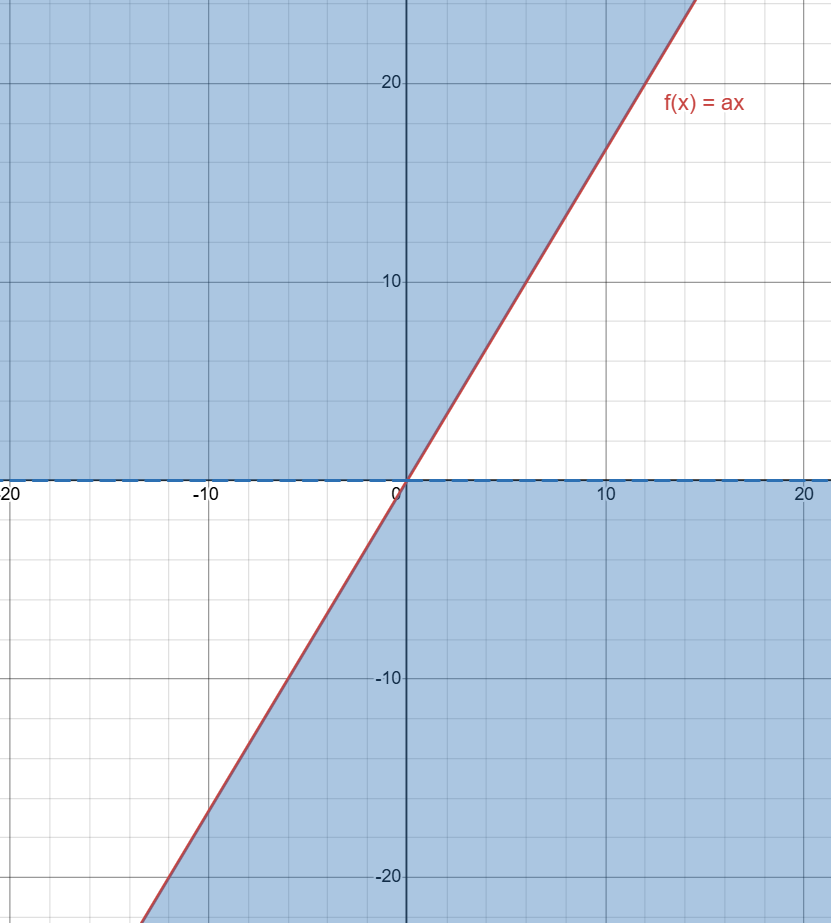
\includegraphics[width=0.45\textwidth]{tasks/10_obszar.png}
\end{center}

Policzymy dystrybuantę, całka musi być liczona po obszarze, który wyznacza wyrażenie
w prawdopodobieństwie (obszar zaznaczony na rysunku):

\[
	P\left(\frac{X}{Y} \le a \right)
\]

Nierówność
\[
	\frac{X}{Y} \le a
\]
jest równoważna
\[
	X \le aY \quad \text{dla } Y>0,
	\qquad
	X \ge aY \quad \text{dla } Y<0.
\]

Ponieważ zmienne losowe \(X\) i \(Y\) są niezależne oraz mają rozkład normalny
\(N(0,1)\), ich wspólna gęstość to iloczyn gęstości i ma postać:
\[
	f_{X,Y}(x,y)=\frac{1}{2\pi}e^{-\frac{x^2+y^2}{2}}.
\]

Dystrybuanta zmiennej \(\frac{X}{Y}\) wynosi więc
\[
	P\left(\frac{X}{Y} \le a\right)
	=
	\int_{0}^{\infty}\int_{-\infty}^{ay}
	\frac{1}{2\pi}e^{-\frac{x^2+y^2}{2}}\,dx\,dy
	+
	\int_{-\infty}^{0}\int_{ay}^{\infty}
	\frac{1}{2\pi}e^{-\frac{x^2+y^2}{2}}\,dx\,dy.
\]

Patrząc na rysunek można dojść do wniosku, że łatwiej przejść po obszarze za pomocą kąta i promienia, a nie współrzędnych kartezjańskich. Wprowadzamy więc współrzędne biegunowe:
\[
	x=r\cos\theta,\qquad y=r\sin\theta,
\]
Wówczas
\[
	x^2 + y^2 = r^2,
	\qquad
	dx\,dy = r\,dr\,d\theta,
\]
a gęstość wspólna przyjmuje postać
\[
	\frac{1}{2\pi} e^{-\frac{r^2}{2}} r\,dr\,d\theta.
\]

\[
	P\left(\frac{X}{Y} \le a\right)
	=
	\int_{0}^{\infty}\int_{\arctan{\frac{1}{a}}}^{\pi}
	\frac{1}{2\pi}e^{-\frac{r^2}{2}}r\,d\theta\,dr
	+
	\int_{0}^{\infty}\int_{\pi + \arctan\frac{1}{a}}^{2\pi}
	\frac{1}{2\pi}e^{-\frac{r^2}{2}}r\,d\theta\,dr.
\]
Wyciągając stałe przed całki otrzymujemy
\[
	P\left(\frac{X}{Y} \le a\right)
	=
	\frac{1}{2\pi}
	\left(
	\int_{0}^{\infty} e^{-\frac{r^2}{2}} r \, dr
	\right)
	\left(
	\int_{\arctan\frac{1}{a}}^{\pi} d\theta
	+
	\int_{\pi + \arctan\frac{1}{a}}^{2\pi} d\theta
	\right).
\]

Najpierw liczymy całkę po zmiennej \(r\):
\[
	\int_{0}^{\infty} e^{-\frac{r^2}{2}} r \, dr
	=
	\left[ -e^{-\frac{r^2}{2}} \right]_{0}^{\infty}
	=
	1.
\]

Teraz liczymy całki po kącie:
\[
	\int_{\arctan\frac{1}{a}}^{\pi} d\theta
	=
	\pi - \arctan\frac{1}{a},
\]
\[
	\int_{\pi + \arctan\frac{1}{a}}^{2\pi} d\theta
	=
	2\pi - \left(\pi + \arctan\frac{1}{a}\right)
	=
	\pi - \arctan\frac{1}{a}.
\]

Zatem
\[
	P\left(\frac{X}{Y} \le a\right)
	=
	\frac{1}{2\pi}
	\left(2\pi - 2\arctan\frac{1}{a}\right)
	=
	1 - \frac{1}{\pi}\arctan\frac{1}{a}.
\]
\[
	P\left(\frac{X}{Y} \le a\right)
	=
	1 - \frac{1}{\pi}\arctan\frac{1}{a} = 1-\frac{1}{\pi} \left(\frac{\pi}{2} -  \arctan{a} \right) = \frac{1}{2} + \frac{1}{\pi}\arctan{a} .
\]
Jest to dystrybuanta rozkładu Cauchy'ego

\subsection*{Odpowiedź}
\[
	\boxed{\frac{X}{Y} \sim Cauchy (0,1)}
\]

\section{Zadanie 11}
Niech \((X, Y)\) będzie punktem wylosowanym jednostajnie ze zbioru
\(\{(x, y) \mid x^2+y^2 \leqslant 1, x \geqslant 0\}\)
(czyli jednostkowego półkola).
Jaki rozkład ma zmienna \(Y/X\)?
\subsection*{Rozwiązanie}
Poprawmy treść zadania i zamieńmy warunek \(x\geqslant0\) na \(x>0\),
aby uniknąć dzielenia przez zero (\(x=0\) i tak jest zdarzeniem
miary zero).

Zauważmy, że wylosowanie punktu jednostajnie z półkola jest równoważne
z wylosowaniem jednostajnie kąta i (już niejednostajnie) odległości
od \((0, 0)\).

Nazwijmy nasze półkole 
\(S = \{(x, y) \mid x^2+y^2 \leqslant 1, x > 0\}\)

\[
    F(z) = \int_{S} [Y/X \leqslant z]~ds
    = \int_{-\frac{\pi}2}^{\frac{\pi}2}
    \int_{0}^{1} 2r[Y/X \leqslant z]~dr~d\alpha
\]

Zdarzenie \([Y/X \leqslant z]\) jest niezależne od \(r\)

\[
    F(z)
    = \int_{-\frac{\pi}2}^{\frac{\pi}2}[Y/X \leqslant z] \int_{0}^{1}
    \frac{2r}{\pi}~dr~d\alpha
    = \int_{-\frac{\pi}2}^{\frac{\pi}2}[Y/X \leqslant z]
    \frac{1}{\pi}~d\alpha
    = \int_{-\frac{\pi}2}^{\frac{\pi}2}[\tan \alpha \leqslant z]
    \frac{1}{\pi} ~d\alpha
\]
\[
    = \int_{-\frac{\pi}2}^{\tan^{-1}z} \frac{d\alpha}{\pi}
    = \frac{1}{\pi} \left(\tan^{-1} (z) + \frac{\pi}2\right)
\]
Jest to dystrybuanta rozkładu Cauchy'ego

\subsection*{Odpowiedź}
\[
\boxed{\frac{Y}{X} \sim Cauchy (0,1)}
\]

\section{Zadanie 12}
\autor{Aleksander Wieczorek}
Czas obsługi i-tego klienta dany jest zmienn¡ losową o wartości oczekiwanej wynoszącej 2 minuty oraz wariancji równej 1 minucie. Zmienne opisujące każdego z
klientów są niezależne. Niech Y oznacza sumaryczny czas obsługi 50 klientów. Wyznacz $P(90 \le Y \le 110)$.
\subsection*{Rozwiązanie}
W tym zadaniu trzeba skorzystać z CTG. Ogranicza się to do tego, że po prostu musimy tak zmodyfikować 
daną nierówność, żeby wyszedł nam wzór z CTG. Wtedy aplikujemy twierdzenie i mamy wynik.\\
Policzmy potrzebne rzeczy:\\
$$Y_i - \text{czas obsługi i-tego klienta}$$
$$Y=\sum_{i=1}^{50} Y_i \qquad \bar{Y} = \frac{Y}{50}$$
$$E(\bar{Y})=\frac{1}{50}E(Y)=\frac{1}{50} \cdot \sum_{i=1}^{50}E(Y_i)=\frac{1}{50} \cdot 50 \cdot 2=2$$
$$Var(\bar{Y})=\frac{1}{50^2}\cdot \sum_{i=1}^{50} Var(Y_i) =\frac{1}{50^2}\cdot 50 \cdot 1 = \frac{1}{50}$$
$$\frac{1}{\sqrt{Var(\bar Y)}}= \sqrt{50}=5\sqrt{2}$$
I teraz wystarczy odpowiednio przekształcić nierówność z treści:
$$P(90 \le Y \le 110) = P\left(\frac{9}{5}\le \bar{Y} \le \frac{11}{5}\right)= P\left(-\frac{1}{5}\le \bar{Y}-E(\bar{Y})\le \frac{1}{5} \right)$$
$$= P\left(-\sqrt{2} \le \frac{\bar{Y}-E(\bar{Y})}{\sqrt{Var(\bar Y )}}\le \sqrt{2} \right)=\Phi(\sqrt{2}) - \Phi(-\sqrt{2})=2\cdot\Phi(\sqrt{2})-1$$
Przedostatnia równość to CTG, a ostatnia wynika z symetrii rozkładu normalnego ($\Phi(-x)=1-\Phi(x)$).\\
Teraz możemy jedynie odczytać dystrybuantę z tabelki.
$$2\cdot\Phi(\sqrt{2})-1 \approx 2\cdot \Phi (1.41) - 1 \approx 0.84 $$

\subsection*{Odpowiedź}
\[
\boxed{\Phi(\sqrt{2}) - \Phi(-\sqrt{2}) \approx 0.84 }
\]

\section{Zadanie 13}
\autor{Oskar Prusik}
Niech \( Y \) będzie zmienną z rozkładu dwumianowego z parametrami \( n = 20 \) oraz \( p = \frac{1}{2} \).
Wyznacz \( P(8 \leq Y \leq 10) \) dokładnie.
Następnie rozpisz \( Y \) jako sumę indykatorów i wyznacz to samo prawdopodobieństwo
za pomocą Centralnego Twierdzenia Granicznego.
Różnica pomiędzy tymi dwoma wynikami wynika z faktu, iż przybliżamy rozkład dyskretny
z małym \( n \) za pomocą rozkładu ciągłego.
Sytuację można poprawić zauważając, że dla \( Y \) zachodzi
\( P(8 \leq Y \leq 10) = P(7.5 \leq Y \leq 10.5) \).
Wyznacz szukane prawdopodobieństwo po zastosowaniu tej poprawki oraz porównaj otrzymane wyniki numerycznie.

\subsection*{Rozwiązanie}

Niech \( Y \sim \mathrm{Bin}\left(n=20, p=\frac12\right) \). Wyznaczamy \( P(8 \le Y \le 10) \).

\subsection*{1. Obliczenie dokładne}
\[
	P(Y=k) = \binom{20}{k} \left(\frac12\right)^{20}, \quad k=0,\dots,20
\]
\[
	P(8 \le Y \le 10) = \sum_{k=8}^{10} \binom{20}{k} \cdot \frac{1}{2^{20}}
\]
\[
	\binom{20}{8}=125970,\ \binom{20}{9}=167960,\ \binom{20}{10}=184756
\]
\[
	P_{\text{exact}} = \frac{125970+167960+184756}{2^{20}} = \frac{478686}{1048576} \approx 0.4565
\]

\subsection*{2. Przybliżenie CTG bez poprawki ciągłości}

Niech \( X_1,\dots,X_{20} \) i.i.d., \( X_i \sim \mathrm{Bernoulli}(1/2) \).
Wtedy:
\[
	\ev{X_i} = \mu = \frac12,\quad
	\variance{X_i} = \sigma^2 = \frac14,\quad
	\sigma = \frac12.
\]

\[
	\bar{X}_{20} = \frac{1}{20}\sum_{i=1}^{20} X_i = \frac{Y}{20}
\]

Z Twierdzenia 15.3.1:
\[
	\lim_{n\to\infty} P\!\left( a \le \frac{\bar{X}_n-\mu}{\sigma/\sqrt{n}} \le b \right) = \Phi(b)-\Phi(a)
\]
Dla \( n=20 \) stosujemy przybliżenie.

Zdarzenie \( \{8 \le Y \le 10\} \) równoważne jest \( \{0.4 \le \bar{X}_{20} \le 0.5\} \).

Podstawiamy do wzoru CTG:
\[
	a = \frac{0.4 - \mu}{\sigma/\sqrt{20}} = \frac{0.4 - 0.5}{0.5/\sqrt{20}}
\]
\[
	b = \frac{0.5 - \mu}{\sigma/\sqrt{20}} = \frac{0.5 - 0.5}{0.5/\sqrt{20}}
\]

Obliczamy liczbowo:
\[
	\sigma/\sqrt{20} = 0.5/\sqrt{20} \approx 0.5/4.472136 = 0.1118034
\]
\[
	a = \frac{-0.1}{0.1118034} = -0.8944272 \approx -0.8944
\]
\[
	b = 0
\]

Zatem:
\[
	P(8 \le Y \le 10) \approx P(-0.8944 \le Z \le 0),\quad Z\sim N(0,1)
\]
\[
	= \Phi(0) - \Phi(-0.8944) \approx 0.5 - 0.1856 = 0.3144
\]

\subsection*{3. CTG z poprawką ciągłości}

Poprawka: \( P(8 \le Y \le 10) = P(7.5 \le Y \le 10.5) \), czyli:
\[
	\left\{ \frac{7.5}{20} \le \bar{X}_{20} \le \frac{10.5}{20} \right\} = \{0.375 \le \bar{X}_{20} \le 0.525\}
\]

Podstawiamy do wzoru CTG:
\[
	a' = \frac{0.375 - 0.5}{0.5/\sqrt{20}} = \frac{-0.125}{0.1118034} = -1.118034 \approx -1.1180
\]
\[
	b' = \frac{0.525 - 0.5}{0.5/\sqrt{20}} = \frac{0.025}{0.1118034} = 0.2236068 \approx 0.2236
\]

Zatem:
\[
	P(8 \le Y \le 10) \approx P(-1.1180 \le Z \le 0.2236)
\]
\[
	= \Phi(0.2236) - \Phi(-1.1180) \approx 0.5885 - 0.1318 = 0.4567
\]
\subsection*{5. Porównanie}
Dokładna wartość: \( 0.4564 \).
CTG bez poprawki: \( 0.3144 \) (błąd \( \approx 0.1420 \)).
CTG z poprawką: \( 0.4567 \) (błąd \( \approx 0.0003 \)).

Przybliżenie CTG z poprawką ciągłości daje wynik bardzo bliski dokładnemu.

\section{Zadanie 14}

Zaprosiłeś na przyjęcie 64 gości. Zakładając, że każdy z nich będzie chciał zjeść niezależnie od pozostałych \(0\), \(1\) albo \(2\) kanapki z prawdopodobieństwami \(\frac{1}{4}, \frac{1}{2}\) oraz \(\frac{1}{4}\) odpowiednio, ile kanapek musisz przygotować, aby mieć \(95\%\) pewności, że ich nie zabraknie?

\subsection*{Rozwiązanie}

Niech \(X_i\) oznacza liczbę kanapek zjedzonych przez \(i\)-tego gościa.
\[
	P(X_i=0)=\tfrac14,\quad P(X_i=1)=\tfrac12,\quad P(X_i=2)=\tfrac14
\]

\[
	\ev{X_i}=1,\qquad \variance{X_i}=\tfrac12
\]

Niech \(S=\sum_{i=1}^{64} X_i\). Wówczas
\[
	\ev{S}=64,\qquad \variance{S}=32,\qquad \sigma_S=\sqrt{32}
\]

Z centralnego twierdzenia granicznego:
\[
	S \approx \mathcal N(64,32)
\]

Szukamy \(s\) takiego, że \(P(S\le s)=0.95\). Mamy
\[
	P(S\le s)=P\!\left(\frac{S-64}{\sqrt{32}}\le \frac{s-64}{\sqrt{32}}\right)
\]

Niech \(Z=\frac{S-64}{\sqrt{32}}\sim\mathcal N(0,1)\). Z tablic:
\[
	P(Z\le 1.645)=0.95
\]

Stąd
\[
	\frac{s-64}{\sqrt{32}}=1.645
	\quad\Rightarrow\quad
	s=64+1.645\sqrt{32}\approx 73.3
\]

Zatem należy przygotować co najmniej \(\boxed{74}\) kanapki.

\section{Zadanie 15 (Filip Manijak)}
Niech $X_1,\dots,X_n$ będzie ciągiem niezależnych zmiennych losowych
z rozkładu wykładniczego z parametrem $\lambda=1$.
Niech $\bar X$ będzie średnią arytmetyczną tego ciągu.
Jak duże musi być $n$, aby
$$
P(0.9 \le \bar X \le 1.1) \ge 0.95 \; ?
$$

\subsection*{Rozwiązanie}
Zmienne $X_i$ mają $E[X_i] = 1, Var[X_i] =1$. Wtedy $S = \frac{\sum X_i}{n}$. Skoro $n$ jest wystraczająco duże, to podstawowe CTG daje nam:
$$
P \left( a \leq \frac{S-1}{\frac{1}{\sqrt{n}}} \leq b \right) = \Phi(b)-\Phi(a)
$$
Ponieważ średnia ma $E[S] = 1, Var[S] = 1/n$.
Przekształcając:
$$
P \left( a \leq \frac{S-1}{\frac{1}{\sqrt{n}}} \leq b \right) = P \left( \frac{a}{\sqrt{n}} +1 \leq S \leq \frac{b}{\sqrt{n}}+1 \right)
$$
Czyli $a \geq -0.1 \sqrt{n}$ oraz $b \leq 0.1 \sqrt{n}$. Minimalne $n$ otrzymamy oczywiście dla najmniejszego $a$ i największego $b$, czyli $ - a = b = 0.1 \sqrt{n} $. Czyli chcemy znaleźć minimalne $n$ że:
$$
\Phi(b) - \Phi(a) = 2*\Phi(b)-1 = 2 * \Phi(0.1 \sqrt{n}) -1 \geq 0.95
$$
Niestety nie da się tego ładnie policzyć, więc sprawdzamy w tablicach. Wychodzi nam, że $\Phi(x) \geq 0.975$ dla $x \geq 1.959964$. Czyli 
$$
0.1 \sqrt{n} \geq 1.959964 \implies n \geq 385
$$

\subsection*{Odpowiedź}
\[
\boxed{\text{385}}
\]

\section{Zadanie 16}
Wskaż, jak można wykorzystać eksperyment, w którym rzucamy \(n\)
razy igłą długości 1 na płaszczyznę z równoległymi liniami narysowanymi
o odstępach jeden,
do oszacowania wartości \(\frac{1}{\pi}\). Jak duże powinno być \(n\),
aby z prawdopodobieństwem \(0.95\) nasze oszacowanie było z~dokładnością
do \(0.01\)? Skorzystaj z CTG.

\subsection*{Rozwiązanie}
Nasze zdarzenie to standardowa igła Buffona,
czyli każdy rzut jest próbą Bernoulliego o prawdopobieństwie
sukcesu \(\frac{2}{\pi}\).

Wartość oczekiwana sumy tych indykatorów po n próbach jest
\(E(\sum_{i=1}^n X_i) = \frac{2}{\pi}n\),\\
a wariancja wyniesie
\(Var(\sum_{i=1}^n X_i) = n \cdot \frac{2}{\pi} \cdot
\left(1-\frac{2}{\pi}\right)\)

Dla średniej mamy: \(E(S) = \frac{2}{\pi}\),
\(Var(S) = \frac{1}{n} \cdot \frac{2}{\pi} \cdot
\left(1-\frac{2}{\pi}\right)\)

Zamiast obliczać \(\frac{1}{\pi}\) z dokładnością \(0.01\)
obliczymy \(\frac{2}{\pi}\) z dokładnością \(0.02\).

Przyjmiemy \(p=\frac{2}{\pi}\), \(\varepsilon = 0.02\)

\[
	P(p-\varepsilon \leqslant S \leqslant p+\varepsilon)
	= P(-\varepsilon \leqslant S-p \leqslant \varepsilon)
\]
\[G
	= P\left(
	-\varepsilon \cdot \sqrt{\frac{\pi^2n}{2(\pi - 2)}}
	\leqslant (S-p) \cdot \sqrt{\frac{\pi^2n}{2(\pi - 2)}}
	\leqslant \varepsilon \cdot \sqrt{\frac{\pi^2n}{2(\pi - 2)}}
	\right)
\]

Kopiując z zadania wyżej (lub sprawdzając w tablicach),\\ widzimy że
\(\Phi(x) \geq 0.975\) dla \(x \geq 1.959964\). Czyli
\[
	0.02 \cdot \sqrt{\frac{\pi^2n}{2(\pi - 2)}}
	\geqslant 1.959964 \implies n \geqslant 2222
\]

Moglibyśmy założyć, że mamy jakąś ograniczoną wiedzę na
temat \(\pi\) (gdybyśmy znali dokładną wartość \(\pi\), obliczenie
\(\frac{1}{\pi}\) mogłoby być wykonane prościej).

Wiedząc jedynie, że \(\pi > 2\), dostalibyśmy \(n \geqslant 2401\)
(pesymistycznym przypadkiem jest tutaj \(\pi = 4\))



\subsection*{Odpowiedź}
\[
	\boxed{\text{2222}}
\]



\chapter{Zestaw 11 -- Sprzęganie łańcuchów Markowa oraz Siła dwu wyborów}
\chaptermark{Zestaw 11}
\graphicspath{{chapters/zestaw-11/}}
\section{Zadanie 1}
\autor{Mateusz Wojaczek}
Niech $P$ będzie macierzą przejścia łańcucha Markowa na skończonej przestrzeni stanów $S$.
Dla $y \in S$ niech $m_y = \min_{x \in S} P(x,y)$.
Skonstruować sprzęganie $\bigl( (X_t, Y_t) \bigr)_{t \in \mathbb{N}}$ dwóch łańcuchów Markowa
z macierzą przejścia $P$ takie, że dla każdego $t \ge 0$ oraz $z \in S$ zachodzi
\[
\mathbb{P}(X_t = Y_t = z) \ge m_z.
\]
\subsection*{Rozwiązanie}
Definiujemy
\[
m = \sum_{y \in S} m_y.
\]

Niech $(X_t, Y_t) = (x,y)$.
Zakładamy, że jeśli łańcuchy się zeszły, to już się nie rozchodzą, tzn.
\[
X_t = Y_t \;\Rightarrow\; X_{t+1} = Y_{t+1}.
\]

W kroku $t \to t+1$ wykonujemy następującą konstrukcję.

Rzucamy monetą. Z prawdopodobieństwem $m$ wypada orzeł. Wtedy
\[
X_{t+1} = Y_{t+1} = x',
\]
gdzie $x'$ wybieramy losowo z rozkładu
\[
\left( \frac{m_i}{m} \right)_{i \in S}.
\]

Z prawdopodobieństwem $1-m$ wypada reszka. Wtedy:
\[
X_{t+1} = x' \quad \text{z rozkładem} \quad
\left( \frac{P(x,i) - m_i}{1-m} \right)_{i \in S},
\]
oraz
\[
Y_{t+1} = y' \quad \text{z rozkładem} \quad
\left( \frac{P(y,i) - m_i}{1-m} \right)_{i \in S}.
\]

Wówczas dla każdego $z \in S$ mamy
\[
\mathbb{P}(X_{t+1} = Y_{t+1} = z)
\;\ge\;
m \cdot \frac{m_z}{m}
=
m_z.
\]

\subsection*{Odpowiedź}
\[
\boxed{\text{ckd}}
\]

\section{Zadanie 2 (Hubert Jastrzębski)}
Rozważmy łańcuch Markowa $(X_t)_{t \in \mathbb{N}}$ na zbiorze $\{0, \ldots, k-1\}$ zdefiniowany następująco. Dla każdego $t \geq 0$, $X_{t+1}$ otrzymujemy z $X_t$ poprzez dodanie wyniku z rzutu sześcienną sprawiedliwą kostką i wzięcie reszty z dzielenia przez $k$. Udowodnij, że dla $k = 10$, $\tau_{\text{mix}} < 100$.

\subsection*{Rozwiązanie}

Dla przypomnienia: \(\tau_{\text{mix}} = \tau_{\text{mix}}(\frac{1}{4})\)

\textbf{Skorzystamy z lematu 10.3.2:}

Niech \(((X_t, Y_t))_{t \in \mathbb{N}}\) to sprzęganie łańcuchów Markowa (skończonych, nieprzywiedlnych, nieokresowych)
z macierzą przejścia \(P\) i zbiorem stanów \(S\).
Niech \(T \in \mathbb{N}\) i \(\epsilon > 0\) będą takie, że dla każdego \(x, y \in S\)
\[\mathbb{P}(X_T \neq Y_T | X_0 = x, Y_0 = y) \leq \epsilon.\]
Wtedy dla każdego \(x \in S\)
\[\tau_{\text{mix}} (\epsilon) \leq T\]

Podstawiając \(T = 99\) i \(\epsilon = \frac{1}{4}\), wystarczy skonstruować sprzęganie takie, że dla każdego \(x, y \in S\)
\[\mathbb{P}(X_{99} \neq Y_{99} | X_0 = x, Y_0 = y) \leq \frac{1}{4}\]

Wtedy dostaniemy, że: 
\(\tau_{\text{mix}} \leq 99\),
co kończy dowód.

\textbf{Aby móc zastosować lemat, zawuażmy, że:}
\begin{enumerate}
    \item Łańcuch Markowa z zadania jest oczywiście skończony (ma 10 stanów)
    \item Łańcuch jest nieprzywiedlny (z każdego stanu można przejść do każdego innego w skończonej liczbie kroków)
    \item Łańcuch jest nieokresowy (z $x$ do $x$ można przejść w 10 krokach (10 $\times$ 1) lub 9 krokach (8 $\times$ 1 + 1 $\times$ 2), a $\gcd(9, 10) = 1$)
\end{enumerate}

\textbf{Konstrukcja sprzęgania:}

Dla dowolnego \(x, y \in \{0, \ldots, 9\}\) definiujemy sprzęganie \(((X_t, Y_t))_{t \in \mathbb{N}}\) łańcucha z zadania, startujące z \((x, y)\):
\begin{enumerate}
    \item Dopóki \(X_t \neq Y_t\), łańcuchy poruszają się niezależnie.
    \item Gdy \(X_t = Y_t\), to łańcuchy poruszają się razem (tzn. \(X_{t+1} = Y_{t+1}\)).
\end{enumerate}

Zauważmy, że dla dowolnego $t$, jeśli \(X_t \neq Y_t\), to prawdopodobieństwo, że \(X_{t+1} = Y_{t+1}\) wynosi co najmniej \(\frac{1}{36}\).

\textbf{Można to prosto udowodnić:}
\begin{enumerate}
    \item Mamy spotkanie, gdy \(X_t + a \equiv Y_t + b \mod 10\), gdzie \(a, b\) to wyniki rzutów kostką.
    \item Jest to równoważne z \(a - b \equiv Y_t - X_t \mod 10\).
    \item Różnica \(Y_t - X_t\) może przyjmować wartości od 1 do 9 (bo \(X_t \neq Y_t\)).
    \item Zbiór możliwych wartości \(a - b\) to \(\{-5, -4, \ldots, 4, 5\} \equiv (\{ 0, 1, \ldots, 9 \})\) (bo \(a, b \in \{1, 2, \ldots, 6\}\)).
    \item Tak więc dla każdej wartości \(Y_t - X_t\) istnieje para \((a, b)\), która spełnia powyższe równanie.
\end{enumerate}

\textbf{Zatem, dla dowolnego} \((x, y)\) startowego, mamy, że prawdopodobieństwo, że łańcuchy się nie spotkają po 99 krokach jest ograniczone przez:
\[\mathbb{P}(X_{99} \neq Y_{99} | X_0 = x, Y_0 = y) \leq (1 - \frac{1}{36})^{99} < \frac{1}{4}\]

Czyli mamy spełnione warunki lematu, a więc \(\tau_{\text{mix}} < 100\).

\section{Zadanie 3}
Niech $P$ będzie macierzą przejścia skończonego, nieprzywiedlnego i nieokresowego
łańcucha Markowa $(M_t)_{t \ge 0}$.
Załóżmy, że istnieją stałe $c < \tfrac12$ oraz $T \ge 0$ takie, że
\[
\tau(c) \le T.
\]
Wówczas dla każdego $\varepsilon > 0$ zachodzi
\[
\tau(\varepsilon)
\le
\left\lceil \frac{\ln \varepsilon}{\ln(2c)} \right\rceil T.
\]

\subsection*{Rozwiązanie}
Rozważmy dwa dowolne stany początkowe $X_0 = x$ oraz $Y_0 = y$.
Z definicji czasu mieszania $\tau(c)$ otrzymujemy
\[
\|P_x^T - \pi\|_{\mathrm{TV}} \le c
\quad \text{oraz} \quad
\|P_y^T - \pi\|_{\mathrm{TV}} \le c.
\]
Stąd, z nierówności trójkąta,
\[
\|P_x^T - P_y^T\|_{\mathrm{TV}} \le 2c.
\]

Na mocy\\
\medskip
\noindent
\textbf{Lematu o sprzęganiu (Lemat 12.3).}
\emph{
Niech $\sigma_X$ oraz $\sigma_Y$ będą rozkładami prawdopodobieństwa
na skończonej przestrzeni stanów $S$.
Niech $Z=(X,Y)$ będzie dowolną zmienną losową o wartościach w $S\times S$,
taką że $X$ ma rozkład $\sigma_X$, a $Y$ ma rozkład $\sigma_Y$.
Wówczas
\[
\Pr(X \neq Y) \ge \|\sigma_X - \sigma_Y\|_{\mathrm{TV}}.
\]
Ponadto istnieje sprzęgnięcie $Z=(X,Y)$, dla którego zachodzi równość:
\[
\Pr(X \neq Y) = \|\sigma_X - \sigma_Y\|_{\mathrm{TV}}.
\]
}
istnieje sprzężenie
\[
Z_{T,x,y} = (X_T, Y_T),
\]
gdzie $X_T$ ma rozkład $P_x^T$, a $Y_T$ ma rozkład $P_y^T$, takie że
\[
\mathbb{P}(X_T \neq Y_T) \le 2c.
\]

Rozważmy teraz nowy łańcuch Markowa $(M'_t)$ o macierzy przejścia $P^T$.
Odpowiada on wykonywaniu $T$ kroków łańcucha $(M_t)$ naraz.
Dla tego łańcucha, przy powyższym sprzęganiu, jeśli dwie kopie łańcucha
$(M'_t)$ startują ze stanu $(x,y)$, to następny stan pary jest zadany
przez rozkład $Z_{T,x,y}$, co implikuje, że prawdopodobieństwo braku
sprzęgnięcia w jednym kroku wynosi co najwyżej $2c$.

Indukcyjnie otrzymujemy, że prawdopodobieństwo, iż sprzężenie łańcucha
$(M'_t)$ nie nastąpi w ciągu $k$ kroków, jest co najwyżej
\[
(2c)^k.
\]

Z lematu o sprzęganiu wynika zatem, że łańcuch $(M'_t)$ jest w odległości
wariacyjnej co najwyżej $\varepsilon$ od swojego rozkładu stacjonarnego
po $k$ krokach, o ile
\[
(2c)^k \le \varepsilon.
\]
Warunek ten jest spełniony dla
\[
k = \left\lceil \frac{\ln \varepsilon}{\ln(2c)} \right\rceil.
\]

Ponieważ łańcuchy $(M_t)$ oraz $(M'_t)$ mają ten sam rozkład stacjonarny,
a każdy krok łańcucha $(M'_t)$ odpowiada $T$ krokom łańcucha $(M_t)$,
otrzymujemy
\[
\tau(\varepsilon)
\le
\left\lceil \frac{\ln \varepsilon}{\ln(2c)} \right\rceil T.
\]

\section{Zadanie 4}
Niech \(G\) będzie \(n\)-wierzchołkowym grafem i niech \(k\) będzie dodatnią liczbą całkowitą taką, że
\[k < \frac{n+2}{\Delta(G)+1}\]
Rozważa,y łańcuch Markowa, gdzie przestrzeń stanów \(\Omega_{k}(G)\) jest rodziną wszystkich \(k\)-elementowych zbiorów niezależnych w \(G\).
Krok ze stanu \(M_{t}\) do następnego stanu działa następująco.
Losujemy jednostajnie i niezależnie: \(v \in M_{t}, w \in V(G)\). Wtedy \(M_{t+1}=m(v, w, M_{t})\) czyli:
jeśli \(M_{t}\textbackslash\{v\}\cup\{w\}\in\Omega_{k}(G)\), to \(M_{t+1} = M_{t}\setminus\{v\}\cup\{w\}\); wpp. \(M_{t+1} = M_{t}\).
Udowodnij, że ten łańcuch jest nieprzywiedlny, nieokresowy i jego rozkład stacjonarny jest jednostajny.

\subsection*{Rozwiązanie}
Do nieprzywiedlność wystarczy pokazać że z \(a\) dasię dojść do dowolnego \(b\).
Pokażemy że z \(a\) dasię dojść do wierzchołka \(c\), który ma więcej wspólnych wierzchołków z \(b\).
Niech \(\{x\} \in b\) oraz \(\{x\} \notin a\) wtedy dopóki ilość krawędzi od \(x\) do wierzchołków z \(a\) większa od 1 to zamieniamy dowolny połączony z \(x\) na niepołączony\(^{*}\).
Jeśli \(\{x\}\) ma dokładnie 1 krawędź do \(a\) to zamieniamy po tej krawędzi, jeśli zero to zamieniamy \(x\) z dowolnym wierzchołkiem z \(a\) którego niema w \(b\).
To zawsze dasię zrobić jeśli \(y\) możemy zamienić na dowolny wierzchołek niepołączony z \(a\textbackslash{y}\cup{x}\),
ilość wszystkich wierzchołków w \(a\textbackslash{y}\cup{x}\) oraz ich sąsiadów będzie co najwyżej \((\Delta(G)+1)k - 2\), bo będzie co najmniej jedna krawędź w środku.
\[(\Delta(G)+1)k - 2 < (\Delta(G)+1)\frac{n+2}{\Delta(G)+1} - 2 = n + 2 - 2 = n\]
Co oznacza że istnieje co najmie jeden taki wierzchołek na który możemy zamienić \(y\).

Nieokresowość mamy z tego że da każdego z \(a\) mamy pętelkę do \(a\) kiedy \(v = w\).

Jeśli \(a, b \in \Omega_{k}(G)\) i istnieje krawędź z \(a\) do \(b\), to istnieje krawędź z \(b\) do \(a\).
Z tego że istnieje krawędź z \(a\) do \(b\), mamy że istnieją \(v \in a\) oraz \(w \in b\), \(v, w \in V(G)\), \(a\textbackslash\{v\}\cup\{w\} = b\).
Wtedy zamieniamy \(v\) z \(w\) miejscami i otrzymujemy krawędź z \(b\) do \(a\).
Także każda krawędź która nie jest pętlą ma to same prawdopodobieństwo i ono jest równe \(\frac{1}{k}\frac{1}{n}\).
Z dwóch powyższych faktów dostajemy że jeśli rozkład będzie jednostajny to on przejdzie sam na siębie, co oznacza że on będzie stacjonarnym.
\section{Zadanie 5}
Niech $G$ będzie skończonym grafem spójnym na co najmniej dwóch wierzchołkach. Rozważmy łańcuch Markowa, gdzie przestrzeń stanów $\Omega(G)$ jest rodziną wszystkich zbiorów niezależnych w $G$. Krok ze stanu $M_t$ do następnego stanu działa następująco. Losujemy jednostajnie i niezależnie: $uv \in E(G)$, $p \in \{1, 2, 3\}$.
\begin{itemize}
    \item Jeśli $p = 1$, to $M'_t = M_t \setminus \{u, v\}$.
    \item Jeśli $p = 2$, to $M'_t = M_t \setminus \{u\} \cup \{v\}$.
    \item Jeśli $p = 3$, to $M'_t = M_t \setminus \{v\} \cup \{u\}$.
\end{itemize}
Jeśli $M'_t$ jest zbiorem niezależnym w $G$, to $M_{t+1} = M'_t$, a w przeciwnym przypadku $M_{t+1} = M_t$. Udowodnij, że ten łańcuch jest nieprzywiedlny, nieokresowy i jego rozkład stacjonarny jest jednostajny.

\subsection*{Rozwiązanie}
Niech $N = |E(G)|$ oznacza liczbę krawędzi w grafie.

\subsection*{1. Nieprzywiedlność}

Łańcuch jest nieprzywiedlny, jeśli z każdego stanu $S$ można dojść do każdego innego stanu $T$ w skończonej liczbie kroków. Ponieważ wykażemy później, że łańcuch jest odwracalny, wystarczy pokazać, że z dowolnego zbioru niezależnego $S$ można dojść do zbioru pustego $\emptyset$.

Wybierzmy dowolny wierzchołek $u \in S$.
\begin{enumerate}
    \item Ponieważ $G$ jest spójny i ma co najmniej 2 wierzchołki, istnieje krawędź $uv \in E(G)$.
    \item Ponieważ $S$ jest zbiorem niezależnym i $u \in S$, to z definicji $v \notin S$.
\end{enumerate}

Wtedy weźmy krok łańcucha, w którym wylosowano krawędź $uv$ oraz $p=1$.
$M' = S \setminus \{u, v\}$. Skoro $v \notin S$, operacja ta redukuje się do $M' = S \setminus \{u\}$. Zbiór $M'$ (jako podzbiór zbioru niezależnego) jest nadal niezależny, więc przejście jest akceptowane z prawdopodobieństwem co najmniej $\frac{1}{3N}$.

Powtarzając tę procedurę dla każdego wierzchołka w $S$, redukujemy zbiór aż do osiągnięcia stanu $\emptyset$. Zatem graf przejść jest spójny.

\subsection*{2. Nieokresowość}

Aby wykazać nieokresowość, wystarczy wskazać stan, dla którego prawdopodobieństwo pozostania w nim w jednym kroku jest dodatnie ($P(S \to S) > 0$).

Niech $S$ będzie dowolnym zbiorem niezależnym. Rozważmy dowolną krawędź $uv$.
\begin{itemize}
    \item \textbf{Przypadek A:} $u \notin S$ i $v \notin S$.
    Jeśli wylosujemy $p=1$, to $M' = S \setminus \{u, v\} = S$. Stan nie ulega zmianie.
    \item \textbf{Przypadek B:} $u \in S$ (wtedy $v \notin S$).
    Jeśli wylosujemy $p=3$ (operacja $M_t \setminus \{v\} \cup \{u\}$), to ponieważ $v \notin S$ i $u \in S$, otrzymujemy $M' = S$. Stan nie ulega zmianie.
\end{itemize}
W obu przypadkach istnieje niezerowe prawdopodobieństwo pozostania w stanie $S$. Zatem łańcuch jest nieokresowy.

\subsection*{3. Jednostajny rozkład stacjonarny}

Aby udowodnić, że rozkład stacjonarny $\pi$ jest jednostajny, wystarczy pokazać, że macierz przejścia jest symetryczna, czyli dla dowolnych stanów $A, B$:
\[ P(A \to B) = P(B \to A) \]
Przejścia zmieniające stan są możliwe tylko między zbiorami różniącymi się w obrębie dwóch wierzchołków

\textbf{Przypadek 1: Zmiana liczby wierzchołków ($|A| = |B| + 1$)} \\
Niech $A = B \cup \{u\}$, gdzie $u \notin B$. Aby przejście było możliwe, $A$ musi być niezależny, więc żaden sąsiad $u$ nie należy do $B$.
\begin{itemize}
    \item \textbf{Przejście $A \to B$ (usunięcie $u$):} Wymaga wylosowania krawędzi $uv$ incydentnej z $u$ oraz $p=1$ ($M' = A \setminus \{u, v\}$). Ponieważ $v \notin A$, usuwamy tylko $u$. Prawdopodobieństwo wynosi:
    \[ P(A \to B) = \sum_{v \in N(u)} \frac{1}{3N} = \frac{\deg(u)}{3N} \]
    \item \textbf{Przejście $B \to A$ (dodanie $u$):} Wymaga wylosowania krawędzi $uv$ incydentnej z $u$. Musimy dodać $u$. W stanie $B$ nie ma $u$ ani $v$.
    Dla $p=3$ operacja to $B \setminus \{v\} \cup \{u\} = B \cup \{u\} = A$.
    Dla $p=2$ operacja to $B \setminus \{u\} \cup \{v\} = B \cup \{v\} \neq A$.
    Zatem interesuje nas tylko $p=3$:
    \[ P(B \to A) = \sum_{v \in N(u)} \frac{1}{3N} = \frac{\deg(u)}{3N} \]
\end{itemize}
Otrzymujemy $P(A \to B) = P(B \to A)$.

\textbf{Przypadek 2: Wymiana wierzchołka} \\
Niech $A$ zawiera $u$, $B$ zawiera $v$, gdzie $uv \in E(G)$, a $A \setminus \{u\} = B \setminus \{v\}$.
\begin{itemize}
    \item \textbf{Przejście $A \to B$:} Wymaga wylosowania konkretnej krawędzi $uv$ oraz $p=2$ ($A \setminus \{u\} \cup \{v\}$).
    \[ P(A \to B) = \frac{1}{N} \cdot \frac{1}{3} = \frac{1}{3N} \]
    \item \textbf{Przejście $B \to A$:} Wymaga wylosowania krawędzi $uv$ oraz $p=3$ ($B \setminus \{v\} \cup \{u\}$).
    \[ P(B \to A) = \frac{1}{N} \cdot \frac{1}{3} = \frac{1}{3N} \]
\end{itemize}
Tutaj również $P(A \to B) = P(B \to A)$.

\textbf{Wniosek:}
Macierz przejścia jest symetryczna, co z poprzedniego zestawu z łańcuchów Markowa wiemy, że daje nam rozkład stacjnonarny, jednostajny.
\section[\nierozwiazane{Zadanie 6}]{Zadanie 6}
Niech \(p, q \in (0, 1)\) takie, że \(p + q = 1\) i niech \(n \geqslant 3\). Rozważ łańcuch Markowa
\((M_t)_{t \in \mathbb{N}}\) na zbiorze wierzchołków \(n\)-wierzchołkowego cyklu taki, że jeśli \(M_t = v\), to
\begin{itemize}
	\item \(M_{t+1} = v\) z prawd. \(\frac{1}{2}\),
	\item \(M_{t+1}\) jest sąsiadem \(v\) zgodnie z wskazówkami zegara z prawd. \(\frac{p}{2}\),
	\item \(M_{t+1}\) jest sąsiadem \(v\) przeciwnie do wskazówek zegara z prawd. \(\frac{q}{2}\).
\end{itemize}
Zauważ, że rozkład stacjonarny \((M_t)_{t \in \mathbb{N}}\) istnieje i jest on jednostajny. Wykaż, że istnieją
dodatnie stałe \(\alpha, \beta\) takie, że
\[
	\alpha n^2 \leqslant \tau_{\text{mix}} \leqslant \beta n^2.
\]
\textit{Wskazówka 1:} nam wyszło \(\alpha = \frac{1}{32}\) i \(\beta = 1\).

\textit{Wskazówka 2 (ograniczenie górne):} Zaprojektuj sprzęganie \((X_t, Y_t)\) takie, że jeśli \(X_t \neq Y_t\),
to tylko jeden łańcuch się ,,porusza'' w danym kroku. Niech \(d_t\) będzie odległością zgodną
z kierunkiem wskazówek zegara pomiędzy \(X_t\) a \(Y_t\). Rozważ jak zmienia się \(d_t\).

\textit{Wskazówka 3 (ograniczenie dolne):} Zamodeluj łańcuch z treści jako łańcuch na \(\mathbb{Z}\). Jako
zbiór \(A_t\) świadczący o tym, że \(\tau_{\text{mix}}\) jest duże, weź połowę cyklu przeciwną do oczekiwanej
projekcji spaceru na \(\mathbb{Z}\) na cykl. Zaaplikuj nierówność Czebyszewa, aby ograniczyć \(P(X_t \in A_t)\).

\brakrozwiazania

\section{Zadanie 7}
Niech \(T_n\) będzie pełnym drzewem binarnym na \(n\) wierzchołkach. Rozważmy spacer losowy po \(T_n\), gdzie z prawdopodobieństwem \(\frac{1}{2}\) stoimy w miejscu, a jeśli mamy wykonać ruch to wykonujemy go jednostajnie na jednego z sąsiadów. Zauważ, że rozkład stacjonarny odpowiednio zdefiniowanego łańcucha Markova istnieje. Pokaż, że \(\tau_{mix}\) jest liniowy w terminach \(n\).\\
\\
\textit{Wskazówka:} Jeśli \(p,q,r \in [0,1]\) takie, że \(p+q+r=1\), \(p \neq q\) i rozważamy spacer na liczbach \([0,n]\) taki, że prawdopodobieństwo pozostania w miejscu to \(r\), prawdopodobieństwo przejścia z \(i\) do \(i-1\) wynosi \(p\), a prawdopodobieństwo przejścia z \(i\) do \(i+1\) wynosi q. Jeśli jesteśmy w punkcie 0 i mamy iść w lewo to zostajemy w miejscu, a jeśli jesteśmy w punkcie \(n\) i mamy iść w prawo to również zostajemy w miejscu. Niech \(X\) będzie zmienną losową będącą liczbą kroków potrzebnych do przejścia z \(n\) do \(0\). Wtedy
\[
	E(X) \leq \frac{1}{p-q}\left[n-q\left(\frac{1-(q/p)^n}{p-q}\right)\right].
\]

\subsection*{Rozwiązanie}

Zacznijmy od rozkładu stacjonarnego. Łańcuch jest skończony i nieprzywiedlny, więc taki rozkład istnieje. \\

Rozważmy teraz sprzęganie łańcuchów Markova \(((X_t, Y_t))_{t\in \mathbb{N}}\), których to macierz przejścia jest określona naszym grafem(możemy ponumerować wierzchołki od \(0\) do \(n-1\)). Określamy \(X_{t+1}, Y_{t+1}\) na podstawie \(X_t, Y_t\) w następujący sposób:
\begin{itemize}
	\item Jeśli \(X_t, Y_t\) były wierzchołkami z różną odległością od korzenia drzewa, to z prawdopodobieństwem \(\frac{1}{2} : X_{t+1} = X_t, \) nastomiast \(Y_{t+1}\) wybieramy jednostajnie spośród sąsiadów \(Y_t\), i z prawdopodobieństwem \(\frac{1}{2}:Y_{t+1} = Y_t, \) nastomiast \(X_{t+1}\) wybieramy jednostajnie spośród sąsiadów \(X_t\).
	\item Jeśli \(X_t, Y_t\) na tym samym poziomie drzewa, to wybieramy ten ruch który wykonujemy na obu tych zmiennych - czyli z prawdopodobieństwem \(\frac{1}{2}\) będzie \(X_{t+1} = X_t, Y_{t+1}=Y_t\), albo wybieramy jednostajnie z sąsiadów tych wierzchołków do którego idziemy(w obu idziemy do lewego dziecka/w obu do rodzica/w obu do prawego dziecka). To zapewnia, że gdy raz \(X_t, Y_t\) będą na jednym poziomie w drzewie, to już zawsze będą na tym samym poziomie.
\end{itemize}
Niech \(Z = Z_1+Z_2\) - oczekiwana liczba kroków po których \(X_t = Y_t\)(tu już chodzi nam o konkretnie ten sam wierzchołek, nie tylko poziom). \\
\\
\(Z_1\) to oczekiwana liczba kroków po których \(X_t, Y_t\) znajdą się na tym samym poziomie. Zauważmy, że \(D_t = |\text{poziom}(X_t)-\text{poziom}(Y_t)|\) możemy sprowadzić do spaceru symetrycznego z dwoma barierami w \(0\) i \(\log_2n\), bo w każdym kroku różnica między poziomami zmienia się o co najwyżej 1. Z przypomnienia o spacerach losowych oczekiwana liczba kroków do uderzenia w 0 niezależnie od miejsca startu mieści się w \(O((\log_2n)^2)\).\\
\\
\(Z_2\) to oczekiwana liczba kroków po których \(X_t = Y_t\) od momentu gdy znajdą się na tym samym poziomie w drzewie. Zauważmy, że jest ona nie większa niż oczekiwana liczba kroków przejścia \(X_t, Y_t\) z liści do korzenia, co znowu możemy zinterpretować przez spacer niesymetryczny z dwoma barierami. Czyli ze wskazówki mamy(u nas \(p = \frac{1}{6}, q=\frac{1}{3})\):
\[
	E[Z_2] \leq \frac{1}{p-q}\left[\log_2n-q\left(\frac{1-(q/p)^{\log_2n}}{p-q}\right)\right] = -6\log_2n - 12 + 12 \cdot 2^{\log_2n} = \theta(n)
\]

Wyżej zostało zamienione \(n\) ze wskazówki na \(\log_2n\), bo tutaj jest spacer ograniczony przez 0 i wysokość drzewa, czyli \(\log_2n\).

Mamy więc, że \(E[Z] \leq cn\) dla pewnego \(c \in \mathbb{R}\).

Korzystamy teraz z lematu \(10.3.2\), przytoczonego m.in. w zadaniu 2. Tutaj mamy(po drodze korzystając z nierówności Markova):
\[
	P(X_t \neq Y_t | X_0 = x, Y_0 = y) = P(Z > t) \leq \frac{E[Z]}{t} \leq \frac{cn}{t}
\]
Dla \(t = 4cn\) mamy:
\[
	P(X_t \neq Y_t | X_0 = x, Y_0 = y) \leq \frac{1}{4}
\]
Więc z lematu dostajemy
\[
	\tau_{mix} = \tau_{mix}(\epsilon) = \tau_{mix}(\frac{1}{4}) \leq 4cn = O(n)
\]


\section{Zadanie 8}
Niech $G$ będzie $n$-wierzchołkowym grafem takim, że stopień każdego wierzchołka to dokładnie $\frac{2}{3} n$ (można założyć, że $ n \leq 3$ i $n$ jest podzielne przez $3$). Rozważmy klasyczny spacer losowy po $G$, gdzie w kroku wybieramy jednostajnie jednego ze swoich sąsaidów. 

(I) Udowodnij, że istnieje rozkład stacjonarny.

(II) Ogranicz, najlepiej jak umiesz czas mieszania $\tau_{\text{mix}}
 $
\subsection*{Rozwiązanie}
(I) Graf jest spójny. Zaużmy, że tak nie jest. Weźmy wierzchołki $u$ i $v$ z dwóch spójnych. Każdy z nich ma $\frac{2}{3}n$ sąsiadów. Z bycia w innych spójnych, konkludujemy, że sąsiedzi są różni. Jeśli zsumujemy sąsaidów $u$ i $v$ otrzymujemy $\frac{4}{3}n$ wierzchołków, co jest sprzecznością, bo graf ma $n$ wierzchołków. 

Równie łatwo, można pokazać, że graf jest nieokresowy. (Graf okresowy może mieć maksymalnie $\frac{1}{4}n^2$ krawędzi, a nasz graf ma $\frac{2}{3}n^2$)

Łatwo też pokazać, że rozkład stacjonarny tego grafu to dla każdego $v$ $\frac{1}{n}$


(II) Wiemy, że $\tau_{\text{mix}}$ = max($\tau_x(\frac{1}{4})$). Gdzie
$\tau_x(\epsilon)$ to minimalny czas $t$, że różnica wektorowa między wektorem w czas $t$, a rozkładem stacjonarnym, znana jako $\Delta_x(t)$.  

Teraz zobaczmy co się dzieje z przy ruchu $t$. Niech zbiór $A$, to zbiór, gdzie wartość jest większa niż rozkład stacjonarny w czasie $t+1$, a $B$ to zbiór, gdzie jest mniejsza. Teraz patrzymy co się wydarzy z wartością wyeksportowaną z wierzchołka $v$. Zaużmy, że w momencie $t$, $v$ miało wartość większą niż w rozkładzie stacjonarmy. Popatrzmy co się dzieję, jeśli połączymy z jamimś wierzchołkiem z $A$, nadwyżka zostanie przekazana. Jeśli natomiast przekażemy do $B$, to zostania zaprzepaszczona. W drugą stronę to działa podobnie. Zeby pokazać, ile zostanie zaprzepaszczone, można wywnioskować następujące równania:
\[
    \frac{\frac{2}{3}n - |A|}{ \frac{2}{3}n}  + \frac{\frac{2}{3}n - |B|}{ \frac{2}{3}n} = \frac{\frac{4}{3}n - |A| - |B|}{\frac{2}{3}n} = \frac{\frac{4}{3}n - n}{\frac{2}{3}n} = \frac{\frac{1}{3}n}{\frac{2}{3}n} = \frac{1}{2}.
\]
Oznacza to, że z każdym minięciem sekundy różnica wektorowa maleje $\frac{1}{2}$ raza. 

W $t = 0$, wszystko znajduję się w jakimś wierzkołku $v$. W $t = 1$, jest w $\frac{2}{3}n$ wartość $\frac{1}{\frac{2}{3}n}$, a w pozostałych $0$. Licząc różnice wektorą mamy:
\[
    \frac{2}{3}n \cdot (\frac{3}{2n} - \frac{1}{n}) + \frac{1}{3}n \cdot (\frac{1}{n} - 0) = \frac{2}{3} \cdot \frac{1}{2} + \frac{1}{3} = \frac{1}{3} + \frac{1}{3} = \frac{2}{3}
\]
W $t = 2$ mamy więc wartość $\leq \frac{1}{3}$, a w $t = 3$ wartość $\leq \frac{1}{6}$, co jest mniejsze niż wymagana $\frac{1}{4}$, z wykładu.

\subsection*{Odpowiedź}
\[
\boxed{\text{3}}
\]

\section[\nierozwiazane{Zadanie 9}]{Zadanie 9}
 (Zadanie 17.2 z książki) Rozważ następujący wariant sekwencyjnego wrzucania
\(n\) kul do \(n\) urn ponumerowanych liczbami od \(0\) do \(n - 1\). Każda przychodząca kula
losuje jednostajnie liczbę \(i \in \{0, 1, \ldots, n - 1\}\), po czym spośród urn \(i, i + 1, \ldots, i + d - 1 \pmod{n}\)
wybiera tę o najmniejszym ładunku. Udowodnij, że dla ustalonego \(d\) maksymalny
ładunek urny po eksperymencie wynosi \(\Theta(\ln n / \ln \ln n)\).

\textit{Uwaga:} W tym zadaniu można założyć, że \(d = 2\) i \(n\) jest dostatecznie duże.

\brakrozwiazania

\section[\nierozwiazane{Zadanie 10}]{Zadanie 10}
 (Zadanie 17.4 z książki) Rozważ następujący wariant sekwencyjnego wrzucania
\(n\) kul do \(n\) urn. Każda przychodząca kula dokonuje \(d\) niezależnych i jednostajnych
wyborów spośród \(n\) urn. Po jej wrzuceniu (do którejś z nich) możemy poprzesuwać kule
w wybranych \(d\) urnach tak, aby jak najbardziej wyrównać ich ładunki. Udowodnij, że
największy ładunek w tej symulacji wynosi co najmniej \(\log_d \ln n - O(1)\) z prawdopodobieństwem \(1 - o(1/n)\).

\textit{Uwaga:} W tym zadaniu można założyć, że \(d = 2\) i \(n\) jest dostatecznie duże.

\brakrozwiazania

\section[\nierozwiazane{Zadanie 11}]{Zadanie 11}

\brakrozwiazania



\end{document}
